\documentclass[12pt,openany]{report}
\usepackage[utf8]{inputenc}
\usepackage[french]{babel}
\usepackage[T1]{fontenc}
\usepackage{awesomebox}
\usepackage[pdftex]{hyperref}
\usepackage{graphicx}
\usepackage{algorithm}
\usepackage{algpseudocode}
\FrenchFootnotes
\usepackage{amsmath}
\hypersetup{
    colorlinks=true,
    linkcolor=blue,
    filecolor=magenta,      
    urlcolor=cyan,
    pdftitle={Memory Sory},
    pdfpagemode=FullScreen
    }

\usepackage{multirow}
\usepackage{color}
\usepackage{amsfonts}
\usepackage{relsize}
\usepackage{array}
\usepackage{bbold}
\usepackage { boxedminipage }
\usepackage{mathtools}

\usepackage{amssymb}


\usepackage[mathcal]{euler}
\graphicspath{ {figures/} }
\usepackage{makeidx}
\usepackage{minitoc}
\newtheorem{theorem}{\underline{Théorème}}
\newtheorem{proposition}{\underline{Proposition}}
\newtheorem{remarque}{\underline{Remarque}}
\newtheorem{definition}{\underline{Définition}}
\newtheorem{lemme}{\underline{Lemme}}
\newtheorem{problem}{\underline{Problème}}
\newtheorem{preuve}{\underline{Preuve}}

\DeclarePairedDelimiter\bra{\langle}{\rvert}
\DeclarePairedDelimiter\ket{\lvert}{\rangle}
\DeclarePairedDelimiterX\braket[2]{\langle}{\rangle}{#1\,\delimsize\vert\,\mathopen{}#2}
\newcolumntype{R}[1]{>{\raggedleft\arraybackslash }b{#1}}
\newcolumntype{L}[1]{>{\raggedright\arraybackslash }b{#1}}
\newcolumntype{C}[1]{>{\centering\arraybackslash }b{#1}}
\setlength{\parindent}{0cm}
\setlength{\parskip}{1ex plus 0.5ex minus 0.2ex}
\newcommand{\hsp}{\hspace{20pt}}
\newcommand{\HRule}{\rule{\linewidth}{0.5mm}}
\newcommand{\tpmod}[1]{{\@displayfalse\pmod{#1}}}
\usepackage{lmodern}
\usepackage{kpfonts}
\usepackage[a4paper,left=2cm,right=2cm,top=2cm,bottom=4cm]{geometry}  
\usepackage{biblatex}




\begin{document} \begin{flushleft}
•
\end{flushleft}

\urlstyle{same}
\baselineskip=18pt
%\maketitle\\
\begin{titlepage}
 \begin{sffamily}
  \begin{center}
   
\includegraphics[scale=0.5]{logo_ugb}~\\[0.8cm]
    \textsc{\LARGE UNIVERSITE GASTON DE BERGER de SAINT LOUIS}\\
    \textsc{Unité de Recherche et Formations des sciences Appliquées}\\
    \textsc{Département de Mathématiques}
    \\[2cm]
    \textsc{\Large Mémoire de Master 2}\\[1.5cm]
    % Title
    \HRule \\[0.4cm]
    {\Large \bfseries CRYPTOGRAPHIE POST-QUANTIQUE: Etude de quelques Algorithmes de Chiffrement basés sur les Codes Correcteurs d'Erreurs admis au concours de NIST 2021 \\[0.4cm] }
    \HRule \\[1cm]
    
\includegraphics[scale=0.4]{ciamitic}
    \\[1cm]
    %Autor and Superviseur
    \begin{minipage}{0.4\textwidth}
     \begin{flushleft} \large
      \textsc{Sory Koné}\\
      Etudiant en master 2 cryptographie,codes et applications
     \end{flushleft}
    \end{minipage}
     \begin{minipage}{0.4\textwidth}
     \begin{flushright} \large
     \emph{Le président du Jury :} \\
     \emph{Examinateur : Pr.} \\
      \emph{encadreur :} Dr Bernadette FAYE\\
      
     \end{flushright}
    \end{minipage}
    \vfill
    %Bottom of the page
    {\large \date{\today} }
    
  \end{center}
  \end{sffamily}
\end{titlepage}

\dominitoc\tableofcontents
\newpage
\listoftables
\listoffigures
\clearpage
\pagenumbering{arabic}



\paragraph{\Huge{Introduction Générale}\\} 

\minitoc

Le codage de canal (numérique) transforme la
séquence d'information utile en une séquence
discrète codée nommée mot de code.\hspace{0.2cm}
En 1948, Shannon \cite{Shannon} a démontré que lorsque le
taux de transmission du système est inférieur à la
capacité du canal de transmission,\hspace{0.2cm} les erreurs
causées par le bruit du canal peuvent être réduites à
un niveau arbitrairement bas par l'utilisation d'un
codage et d'un décodage approprié.\hspace{0.2cm} À partir de ce
moment-là,\hspace{0.2cm} les chercheurs ont commencé à étudier
différentes méthodes de construction des codes
correcteurs d'erreurs

Un code correcteur d'erreurs est un système qui permet de détecter et/ou corriger les erreurs qui peuvent se produire lors de la transmission ou du stockage de données numériques.\hspace{0.2cm} Voici un schéma général du fonctionnement d'un code correcteur d'erreurs.
\begin{flushleft}



\textbf{ Encodage} : Les données d'entrée sont divisées en blocs de données.\hspace{0.2cm}
Un algorithme d'encodage transforme chaque bloc de données en un bloc de données plus long,\hspace{0.2cm} en ajoutant des bits de redondance (appelés bits de parité) aux données d'origine.\hspace{0.2cm} Ces bits supplémentaires sont calculés de manière à créer des caractéristiques spécifiques permettant de détecter et/ou corriger les erreurs.\\
 \textbf{ Transmission ou stockage} : Les blocs de données encodés sont transmis sur un canal de communication ou stockés dans un support de stockage.\\
\textbf{ Réception ou récupération} : Les blocs de données encodés sont reçus ou récupérés depuis le support de stockage.\\
\textbf{  Détection d'erreurs} : Lors de la réception,\hspace{0.2cm} le décodeur vérifie les bits de redondance pour détecter si des erreurs se sont produites lors de la transmission ou du stockage.\hspace{0.2cm} Il compare les bits de parité calculés à ceux reçus pour détecter les différences.\\
 \textbf{ Correction d'erreurs (si possible) }:\hspace{0.2cm}Si des erreurs sont détectées et que le code correcteur d'erreurs est capable de corriger ces erreurs,\hspace{0.2cm} l'algorithme de décodage peut utiliser les bits de redondance pour corriger les erreurs et récupérer les données d'origine.\\
\textbf{ Récupération des données d'origine }:Après la détection et/ou la correction des erreurs, \hspace{0.2cm}les données d'origine sont récupérées à partir des blocs de données encodés et des bits de redondance.\\
Il existe différents types de codes correcteurs d'erreurs, \hspace{0.2cm}tels que les codes de Hamming,\hspace{0.2cm} les codes cycliques, les codes de Reed-Solomon,\hspace{0.2cm} les turbo codes, les codes LDPC et les codes polaires,\hspace{0.2cm} qui utilisent diverses techniques pour détecter et corriger les erreurs.

\end{flushleft}
Il est essentiel de noter que l'utilisation de codes correcteurs d'erreurs en combinaison avec le chiffrement ne doit pas être considérée comme une méthode de chiffrement à part entière,\hspace{0.2cm} mais plutôt comme un moyen d'améliorer la fiabilité et l'intégrité des données chiffrées.\hspace{0.2cm} Le chiffrement assure la confidentialité,\hspace{0.2cm} tandis que les codes correcteurs d'erreurs améliorent la robustesse des données face aux erreurs.\\
 Le choix d'un code correcteur d'erreurs dépend des exigences spécifiques de l'application,\hspace{0.2cm} telles que la quantité d'erreurs attendue et les contraintes de performance et de complexité.\\De ce fait,\hspace{0.2cm} en 1978 Robert  McEliece a dévoloppé un système de codage basé sur le code de Goppa Binaire mais à cause de la taille des clés publiques celui-ci a été abandonné en faveur du système de RSA.\\ 
 Cependant,\hspace{0.2cm}au bout de deux décennies les progrès récents de l’informatique quantique ont  posé un sérieux problème pour la cryptographie traditionnelle à clé publique,\hspace{0.2cm} dont la sécurité repose sur la dureté de la factorisation de grands entiers et de calcul des logarithmes discrets dans un groupe cyclique.\\
 En fait
l’algorithme de Shor [1] peut calculer la factorisation entière
et les opérations logarithmiques discrètes en temps polynomial sur un ordinateur quantique,\hspace{0.2cm} réduisant ainsi considérablement la marge de sécurité
  primitive actuelle de cryptographie à clé publique.\hspace{0.2cm}
Pour faire face à la menace de la machine quantique,\hspace{0.2cm} les cryptanalystes se sont lancés dans l'élaboration de nouveaux cryptosystèmes qui ne seront basés sur le problème du logarithme discret et la durée de factorisation des grands nombres:\hspace{0.2cm} C'est l'ère de la cryptographie post-quantique.\hspace{0.2cm}La recherche de cryptosystèmes post-quantiques s'effectue dans les domaines des codes correcteurs d'erreurs,\hspace{0.2cm} les courbes élliptiques,\hspace{0.2cm} l'isogénie entre autres et plusieurs résultats s'en ont suivis.\hspace{0.2cm}Ainsi le concours de NIST lancé en 2016 visant à sélectionner un ou plusieurs algorithmes de chiffrement post-quantique sûrs et efficaces,\hspace{0.2cm} qui seraient largement acceptés et implémentés dans les systèmes d'information à l'avenir.\hspace{0.3cm} Celui-ci est à son quatrième tour de 2017 à 2021 à l'issu duquel il a été retenu que 3 chiffrements dans le domaine des codes correcteurs d'erreurs que sont : le McElièce classique, \hspace{0.2cm}le BIKE(Bit-flipping Key Encapsulation) et le HQC (Hamming Quasi Cyclic). \\
Au cours de notre rédaction nous aborderons dans le chapitre I les notions mathématiques sur lesquelles se sont fondées les candidats et leur base de sécurité. \\ Dans le chapitre II , nous parlerons de la cryptographie de 1978 à nos jours en relevant les travaux et les améliorations effectués dans le domaine des codes correcteurs d'erreurs.\\
Dans le chapitre III nous évoquerons   NIST et son concours à savoir son objectif et les critères de sélection des candidats en  faisant leur cryptanalyse détaillée. \\ Dans le chapitre IV nous étudierons les algorithmes d'attaques sur les candidats  en mettant en exergue les structures mathématiques et informatiques sur lesquels ils se fondent.\\ Dans le dernier chapitre nous allons faire une étude comparative des avantages et inconvénients des candidats et donner une implémentation d'un candidat.






\chapter{La cryptographie de 1978 à Nos jours  : De RSA à Mc Elièce}
\minitoc
\newpage

En 1976, Diffie et Hellman ont publié l'idée de la clé publique ou de la cryptographie asymétrique. Jusqu'à cette époque, la cryptographie était basée sur l'idée de la cryptographie symétrique dans laquelle l'expéditeur et le destinataire devaient avoir une clé secrète partagée pour pouvoir
 communiquer en toute sécurité. La cryptographie asymétrique permet à un expéditeur de chiffrer un
message avec une clé publique publiée qui ne peut être déchiffrée que par quelqu'un qui
avait une clé privée associée.
Les premiers schémas basés sur ce message étaient RSA
et McEliece  tous deux publiés en 1978. RSA a basé sa sécurité sur la dureté de
factoriser de grands nombres et McEliece a basé sa sécurité sur le problème du décodage
un code Goppa aléatoire.
RSA a été préféré à McEliece comme l'un des schémas de cryptographie asymétrique les plus populaires des 40 dernières années, principalement en raison de la petite taille de sa clé publique par
comparaison.
 
En 1994, Shor a proposé quelques algorithmes pour les ordinateurs quantiques qui
a rendu les problèmes auparavant irréalisables sur le plan informatique de la factorisation de grands nombres
et trouver des logarithmes discrets de nombres dans des anneaux modulaires est soudainement faisable.

 
Dans
les décennies suivantes, cela n'a pas eu beaucoup d'effet sur la popularité du RSA en tant que
norme de cryptage asymétrique. Mais, maintenant avec l'avènement des ordinateurs quantiques
de tailles de bits croissantes, ce problème est revenu. Dans le même temps, les grandes tailles de clé
requis par les systèmes basés sur des codes ne sont plus autant un problème en raison de l'augmentation
accès aux réseaux à haut débit.\hspace{0.2cm}Nous avons plusieurs classes de codes :\\
Les codes polaires sont une classe de codes correcteurs d'erreurs qui ont été introduits par Erdal Arikan en 2009. Ils se sont avérés être une avancée significative dans le domaine des codes correcteurs d'erreurs et ont attiré beaucoup d'attention depuis leur création. Ces codes sont devenus un élément clé dans les normes de communication numérique avancées telles que le 5G.\\
Turbo codes : Les turbo codes, introduits par C. Berrou, A. Glavieux et P. Thitimajshima en 1993, ont révolutionné les performances des codes correcteurs d'erreurs. Ils sont basés sur l'utilisation de deux ou plusieurs codes correcteurs d'erreurs en parallèle, combinés avec un schéma d'itération itératif pour améliorer considérablement les performances de décodage.

Codes LDPC : Les codes LDPC (Low-Density Parity-Check), proposés à l'origine par Robert Gallager dans les années 1960, ont été redécouverts dans les années 1990 par David MacKay. Ces codes utilisent des matrices creuses et présentent des performances de décodage proches des capacités théoriques des canaux de communication.

Codes polaires : Les codes polaires, introduits par Erdal Arikan en 2009, ont été un autre développement majeur dans les codes correcteurs d'erreurs. Comme mentionné précédemment, ils permettent d'atteindre la limite de la capacité de Shannon de manière asymptotique et ont été adoptés dans les normes de communication 5G.

Codes Turbo-product : Les codes Turbo-product sont une extension des turbo codes et des codes LDPC, proposée par Claude Berrou en 2006. Ils permettent d'obtenir de très bonnes performances en utilisant des décodeurs simplifiés.

Codes polynomiaux : Les codes polynomiaux, introduits en 2007 par O. Ytrehus, sont une autre classe de codes correcteurs d'erreurs qui ont des performances prometteuses dans certains scénarios.

Ces améliorations ont contribué à faire évoluer les codes correcteurs d'erreurs vers des performances de plus en plus élevées, tout en réduisant la complexité des décodeurs. Ils sont largement utilisés dans une multitude d'applications, allant des communications numériques (télécommunications, Internet) aux systèmes de stockage de données (disques durs, mémoires flash) en passant par les communications spatiales et les systèmes embarqués.


En 2016, le National Institute of Standards and Technology (NIST) a publié une
appel à propositions pour des cryptosystèmes post-quantiques qui ne seraient pas basés sur le
difficulté à factoriser de grands nombres ou à trouver des logarithmes discrets .\\
Dans ce qui suit, nous rappelons quelques notions de bases sur les codes. 

\section{Arithmétique des codes correcteurs d'erreurs}
\subsection{Code correcteur d'erreur}
Un code correcteur d'erreur est une technique de codage basée sur la redondance. Elle est destinée à corriger les erreurs de transmission d'une information sur un canal de communication peu fiable.\\
\textbf{Exemple}:
\begin{enumerate}
\item $0101 \rightarrow 01010101$ code à répétition
\item Alpha Tango Charlie $\rightarrow$ ATC
\item TCP-IP (Internet)
\end{enumerate}
\textbf{Codage avec redondance}
\begin{itemize}
\item Soit un message initial $u=(u_1,u_2,u_3,...,u_k)$
\item Une fonction $\varphi(u)=w=(w_1,w_2,...,w_r)$
\item message reçu $(u,w)=(u_1,u_2,...,u_k,w_1,w_2,...,w_r)$

\end{itemize}
w: la redondance\\
r: la longueur de w\\
$(w_1,w_2,...,w_r)$: Les bits de contrôle\\
Corriger: Il faut que $\varphi^-1$ existe $\rightarrow$ $\varphi$ est existe \\
Chaque mot de code est de longueur $n=k+r$. L'ensemble de tous les mots obtenus de cette façon forme un \textbf{code} de \textbf{longueur} $n$ et de \textbf{dimension} $k$.\\

\textbf{Notation}: $\varphi$ est la fonction de codage\\
                    $Im\varphi$ est le code\\
- Détecter une erreur:\\
$(u,w)=(u_1,u_2,...,u_k,w_1,w_2,...,w_r)$\\
$S(u)=\varphi(u_1,u_2,...,u_k)-w_1,w_2,...,w_r=0$ \\
$\varphi(u_1,u_2,...,u_k)\neq( w_1,w_2,...,w_r)$\\
\textbf{Calcul du Syndrôme}\\
$\varphi(u_1,u_2,...,u_k)=(y_1,y_2,...,y_r)$\\
$S(u)=(y_1-w_1,y_2-w_2,...,y_r-w_r)$
\begin{itemize}
\item Si $S(u)\neq 0 \rightarrow$ Il y'a erreurs.
\item $S(u)= 0 \rightarrow$ Il n'y a pas d'erreus
\end{itemize}
\subsection{ Capacité de détection }
Un code $\mathit{\textbf{C}}$
 de longueur $n$ est dit \textbf{t-détection} (\textbf{e-correction)} s'il permet de détecter \textbf{t erreurs} (resp. \textbf{e-erreurs}).\\
\subsection{Distance de Hamming}
Soit $\mathbf{F}$ un alphabet fini, pour deux éléments de $\mathbf{F}$ on appelle distance de Hamming de $X$ et $Y$ le nombre de composantes pour lesquelles $X$ et $Y$ différent: \\
Elle est notée $d(X,Y)=:card{\lbrace i \in \lbrace 1,...,n\rbrace / x_i \neq y_i\rbrace}$. \\
\textbf{Exemple}: $ \mathbb{F}={1,2,3,4,5}$ et $ n=5$\\
Soient $X=(0,1,2,3,1)$ et $Y=(0,2,1,3,1)$, la distance de Hamming de $X$ et $Y$ est  $d(X,Y)=2$.\\
L'application $d:\mathbf{F}^n x \mathbf{F}^n \rightarrow \mathbf{N}$\\
$(x,y)\rightarrow d(x,y)$\\
d est une distance
\begin{enumerate}
\item $d(x,y)\geq 0$
\item $ d(x,y) = d(y,x)$
\item $d(x,z)\leq d(x,y) + d(y,z)$
\item si $d(x,y)=0 \rightarrow x=y$
\end{enumerate}
\subsubsection{Poids de Hamming}
On appelle le poids de Hamming noté $\omega(m)$, le nombre de bits non nuls de $m$.\\
\textbf{Exemple}: $\omega(0,1,1)=2$\\
\begin{proposition}
Soit $\mathbf{C}$ un code longueur $n$ est  $\mathbf{C}$ est t-correcteurs s'il peut corriger t-erreurs\\ $\forall x \in \mathbf{F}^n , card \lbrace c \in \mathbb{C} / d(x,c)\leq t \rbrace  \leq 1$.\\
\end{proposition}
\begin{remarque} Pour pouvoir corriger, il faut que $\mathbf{c}$ soit l'unique mot de code le plus proche de $x$.
\end{remarque}

\subsubsection{La distance minimale d'un code}
C'est la plus petite distance entre les mots de $\mathbf{C}$. \\On le note : 
$d_H \left( \mathbf{C} \right)=min\lbrace d(x,y)/ x,y \in \mathbf{C}^2 , x \neq y \rbrace $.\\

\textbf{Notation:}
Si \textbf{C} est de cardinal m , de longueur n et distance minimale d, on dit que \textbf{C} est un \textbf{(m,n,d)-code}.\\
\subsection{Codes linéaires}
Un code linéaire est caractérisé par:
\begin{itemize}
\item Matrice génératrice, Matrice de contrôle
\item Code systématique
\item décodage d'un code linéaire
\item Syndrome
\end{itemize}
\textbf{Exemple}
\begin{enumerate}
\item Code de Hamming
\item Codes cycliques
\item Codes BCH
\item de Reed Salomon
\end{enumerate}
\subsubsection{ Un code linéaire}
\begin{definition}Un code linéaire de longueur $n$ est un sous espace vectoriel $ \mathbf{C} \in \mathbb{F}_2^k $. La lettre $k$ désigne la dimension, le nombre de mot de code est $2^k$. le poids $ \omega\left( x\right) = \left\lbrace i / x_i \neq 0\right\rbrace $.
\end{definition}
\textbf{\underline{Notation}: } \textbf{C} est un code (n,k,d).\\
Si $\mathbb{F}=\mathbb{F}_2=\left\lbrace 0,1\right\rbrace , \forall n > 0 $, si l'on pose $ m=2^n $, l'application \\
\begin{center}


 $\varphi: \mathbb{F}^n \rightarrow \mathbb{Z}/m\mathbb{Z}$\\ 
 $(c_0,c_1,...,c_n) \rightarrow c_0+2c_1+...+2^{n-1}c_{n-1}$
 \end{center}

est une bijection .
\begin{definition} Un code de longueur $n$ et de dimension $k$ est sous espace vectoriel de dimension $k$ de $\mathbb{F}_q^n$.
\end{definition}
\begin{proposition} Si $\mathbf{C}$ est un code linéaire, l'ensemble des distances entre les mots de code de $\mathbf{C}$ est l'ensemble des poids des mots de $\mathbf{C}$.
\end{proposition}
\textbf{\underline{Preuve}: }\\ Soient $x,y \in \mathbf{C}$ alors $x.y \in \mathbf{C}$ car $\mathbf{C}$ est un sous espace vectoriel.\\
$ d\left( x,y\right) = \omega \left( x-y\right)$.\\
Donc toute distance est un poids d'un mot de $\mathbf{C}$.\\
Réciproquement si $x$ est un mot de $\mathbf{C}$,
$ \omega\left( x\right)=d\left(x , 0\right).$\\
Donc tout poids est une distance de mots de $\mathbf{C}$.\\
\textbf{\underline{Conséquence}:} La distance \textbf{minimale} de $\mathbf{C}$ est égale au plus petit poids des mots de $\mathbf{C}$.\\
\textbf{\underline{Remarque}:}
\begin{enumerate}
\item Cette conséquence nous donne une amélioration dans la recherche de la distance minimale.
\item Un code linéaire est entièrement déterminé par une base (k-mot de code)
\end{enumerate}

Ceci nous conduit à la notion de matrice génératrice.
\subsubsection{\underline{Une matrice génératrice}}

Une matrice génératrice $\mathit{G}$ d'un code $(n,k)$ linéaire, la matrice $ k x n$ de rang k dont les lignes forment une base de $\mathbf{C}$.\\
Alors on a: $\mathbf{C}= m \times \mathbf{G}$, $ m \in \mathbb{F}_2^{k} $.\\
L'application $m \rightarrow m\mathit{G}$ est un isomorphisme de $\mathbb{F}_2^k$ sur 
$\mathbf{C}$.\\

\subsubsection{La matrice de contrôle de Parité}
\begin{definition}
La matrice de contrôle peut être vue comme la matrice génératrice du code dual
\begin{center}

$\mathit{C}^{\perp}=\left\lbrace y \in \mathbb{F}_2^{n}, \forall c \in \mathit{C}, \hspace{0,2cm} y \cdot c=0  \right\rbrace   $
\end{center}
où $ \cdot \hspace{0,2cm}$ est le produit scalaire usuel.
\end{definition}
\begin{proposition}
Soit $\mathbf{H}$ une matrice de contrôle du code $\mathit{C}$. La distance minimale $d$ de $\mathit{C}$ est caractérisée par les propriétés suivantes:
\begin{itemize}
\item[•] $d-1$ colonnes de $\mathbf{H}$ sont toujours linéairement indépendantes.
\item[•] il y a un système de $d$ colonnes de $\mathbf{H}$ qui est lié.
\end{itemize}
\end{proposition}
\textbf{\underline{Preuve}}\\ Supposons que $d-1$ colonnes de $\mathbf{H}$ sont toujours linéairement indépendantes.
Soit $c = (c_1,\cdots , c_n)$ un mot de code. On a $\mathbf{H}^tc = 0$. Si $w(c) < d$ alors on a relation entre moins de $d$ colonnes de $\mathbf{H}$. Inversement un mot $c$ de poids $d$ donne une relation entre $d$ colonnes de $\mathbf{H}$.

\subsection{Codes de Reed-Solomon Généralisés  }

\begin{definition} (Codes de Reed-Solomon Généralisés)\\
Soient un entier $m\geq 1$, $n$ un entier et $q$ une puissance d'un nombre premier tels que $n\leq q^m$.\\
Soient $x=(x_1,\cdots,x_n)\in \mathbb{F}_{q^m}^n$ tels que $ x_i \neq x_j, i, j=1, \cdots,n $ si $ i \neq j $ et $ v=(v_1,\cdots,v_n) \in \mathbb{F}_{q^m}^{*n}$(chaque $v_i$ est non nul). Le code de Reed-Solomon Généralisé de longueur $n$, de dimension $k$, de support $x$ et de multiplieur  $v$, noté $GRS_k (x,v)$ est :
\begin{center}
$ 
GRS_k(x,v)=\lbrace ( v_1f(x_1),\cdots,v_nf(x_n) ): f \in \mathbb{F}_{q^m}[x]: deg(f)<k \rbrace
$
\end{center}
\end{definition}

\begin{proposition}
Soit un code de Reed-Solomon généralisé $GRS_k(x,v) $ de matrice de contrôle $ \mathbf{H}$.\hspace{0.2cm} Alors la matrice $\mathbf{H}$ est sous la forme :\\
\begin{center}
$
\mathbf{H}=
\begin{pmatrix} 
         
         v_1 & v_2 & \cdots & v_n \\
         v_1 x_1 & v_2 x_2 & \cdots & v_n x_n \\
         
         v_1 x_1^2 & v_2 x_2^2 & \cdots & v_n x_n^2 \\
      \vdots & \vdots & \vdots &   \vdots \\
      v_1 x_1^{k-1} & v_2 x_2^{k-1} & \cdots & v_n x_n^{k-1}
         
   \end{pmatrix}$

\end{center}

Une matrice de contrôle d'un code de Reed-Solomon généralisé est le produit d'une matrice de vandermonde et d'une matrice diagonale.\\
Soit $\mathbf{H} $ une matrice de parité d'un code $ GRS_k(x,v).$\\
On a : $\mathbf{H} = \mathbf{V}_{n-k,n}^{(x)}\cdot \mathbf{D}_v$ où $\mathbf{V}_{n-k,n}^{(x)}$ est une matrice de Vandermonde et $\mathbf{D}_v=diag(v_1,\cdots,v_n)$ est une matrice diagonale avec
\begin{center}
\scalebox{1}

$\mathbf{V}_{n-k,n}^{(x)}=\left (\begin{smallmatrix}
 1 & 1 & \cdots & 1 \\ x_1 &  x_2 & \cdots & x_n \\ x_1^2 &  x_2^2 & \cdots &  x_n^2 \\\vdots & \vdots & \vdots &   \vdots \\x_1^{k-1} & x_2^{k-1} & \cdots &  x_n^{k-1}
\end{smallmatrix}\right)$ \hspace{0.3cm} et \hspace{0.3cm}
\scalebox{1}
{$\mathbf{D}_v =\begin{pmatrix}  
 v_1 & 0 & \cdots & 0 \\0 &  v_2 & \cdots & 0 \\ \vdots & \vdots & \vdots &   \vdots \\ 0& 0 & \cdots &  v_n \end{pmatrix}$}.

\end{center}
   
    
    Tout code linéaire $\mathit{C}$ satisfait à la borne de Singleton. Autrement dit, si $\mathit{C}$ est un $[n,k,d]$-code linéaire, alors $ d\leq n-k+1$. En particulier, un code de Reed-Solomon généralisé vérifie aussi cette condition. La proposition suivante énonce une propriété particulière qu'ont les codes GRS: le critère d'optimalité MDS.
\end{proposition}    
    
    \begin{proposition} Un code de Reed-Solomon généralisé est MDS (Maximum Distance Separable)\cite{Ndollane}. \end{proposition}
    \paragraph{\underline{Preuve}\\}
    Soit $\mathit{C} $ un code $GRS_k(x,v)$ sur $\mathbb{F}_q$ de paramètres [n,k,d].Alors $d\leq n-k+1$ (Borne de Singleton).\\
    Soit $c \in \mathit{C}$,alors $\exists f \in \mathbb{F}_q[x]$ avec $deg(f)\leq k-1 $ tel que $c=(v_1 \cdot f(x_1),v_2 \cdot f(x_2),\cdots,v_n \cdot f(x_n))$.\\
    Un polynôme de degré inférieur à $k$ a au plus $k-1$ racines. Donc $c$ a au moins $n-k+1$ composantes non nulles. Ainsi le poids de Hamming de $c$ est supérieur ou égal à $n-k+1$($ w_H(c)\geq n-k+1 $.)\\
    D'où le poids minimal du code $\mathit{C}$ est supérieur ou égal à $ n-k+1$.Etant donné que le poids minimal d'un code linéaire est égal à sa distance minimale, alors $ d \geq n-k+1$. Par suite,
    $ d = n-k+1$.\\
    \textbf{\underline{Exemple }:} Considérons le corps
    $\mathbb{F}_8=\mathbb{F}_2[x]/(x^3 + x+1)$. Soit $\alpha$ un élément primitif de $ \mathbb{F}_8$.\\
    Le code \\
    $\mathit{C}=\left\lbrace   \left( 
    \alpha^3 \cdot f(\alpha^5),f(\alpha^2),\alpha \cdot f(1),\alpha \cdot f(\alpha^4),f(\alpha^3),\alpha^2 \cdot f(0),\alpha^5 \cdot f(\alpha^6),f(\alpha) \right)| f \in \mathbb{F}_8[x]: deg(f)<3   \right\rbrace  $\\
    est un code de Reed-Solomon généralisé sur $\mathbb{F}_8$ de paramètres $[8,3,6] $, \\ de support $x=(\alpha^5,\alpha^2,1,\alpha^4,\alpha^3,0,\alpha^6,\alpha) $ et de multiplieur $v=(\alpha^3,1,\alpha,\alpha,1,\alpha^2,\alpha^5,1 ) $. Une matrice génératrice $\mathbf{H} $ du code $GRS_3(x,v)$ est :
    \begin{center}
    
    
    $\begin{pmatrix} 
         
         \alpha^3 &1&\alpha&\alpha&1&\alpha^2&\alpha^5&1\\
         \alpha&\alpha^2&\alpha&\alpha^5&\alpha^3&0&\alpha^4&\alpha\\
         \alpha^6&\alpha^4&\alpha&\alpha^2&\alpha^6&0&\alpha^3&\alpha^2
   \end{pmatrix}$.
   
   \end{center}
  \begin{definition} \textbf{(Polynôme de Lagrange)}\\
   Soient $(\alpha_0,\cdots,\alpha_{n-1})\in \mathbb{F}_q^n $
   avec $\alpha_i \neq \alpha_j $ si $ i \neq j$. Définissons les polynômes de Lagrange par :\\
   
   \begin{center}
   $ \forall i \in [0, n-1] \mathbf{L}_i[x]={\Huge \Pi}_{j \in [0, n-1], j \neq i }(x-\alpha_j) \in \mathbb{F}_q[x]_n $.
 
   
   \end{center}
     \end{definition}
    En plus d'être des codes MDS, les codes GRS ont encore une autre propriété: le dual d'un code GRS est aussi un code GRS de même support(mais pas de même multiplieur).\\
    \paragraph{Propriété:\\}
    Le dual d'un code $GRS_k(\alpha,v)$ est le code $GRS_{n-k}(\alpha,v')^{\perp} $ où $v' \in \mathbb{F}_q^{*n} $ tel que\\
    
    \begin{center}
    $ \forall i \in [0, n-1], v_i^{'}= v_i^{-1} \mathbf{L}(\alpha_i)^{-1}$
    \end{center}
    \paragraph{Remarque: \\}
    Si $ n=q-1 $, on dit que le code de Reed-Solomon généralisé est primitif.
    Si $ v_i =1 \forall i \in \lbrace 1, \cdots,n \rbrace $, on dit que le code est normalisé. On obtient ainsi un code de Reed-Solomon tout simplement.\\
    Donnons la définition d'une fonction d'évaluation. Soit $\alpha_1,\cdots,\alpha_n \in \mathbb{F}_q $ deux à deux distincts, avec $n<q $.
    \begin{definition}
    La fonction d'évaluation associée à $\alpha_1,\cdots,\alpha_n  $ est : 
    \begin{center}
     
      $ ev:\mathbb{F}_q[x]\longrightarrow \mathbb{F}_q^n $\\
       $ \hspace{3cm} f    \longrightarrow \left(  f(\alpha_1),\cdots,f(\alpha_n)  \right)$.   
    
    \end{center}
    \end{definition}
    
  \subsubsection{Code de Reed-Solomon}  
  \begin{definition}\cite{Ndollane}p44\\
  Soient $\alpha_1,\cdots,\alpha_n \in \mathbb{F}_q $, avec $n<q $ et 
  $ \alpha_i \neq x_j $ si $i \neq j $, et $ev$ la fonction d'évaluation associée à $\alpha_1,\cdots,\alpha_n  $. Soit \\
  \begin{center}
  $ \mathbf{L}_k=\left\lbrace f \in \mathbb{F}_q[x]: deg f <k \right\rbrace  $,
  \end{center}
  l'ensemble des polynômes de $\mathbb{F}_q[x] $ de degré strictement inférieur à $k$.\\
  Le code de Reed-Solomon de dimension $k$ et de support $\alpha=(\alpha_1,\cdots,\alpha_n) $, noté $RS(\alpha,k)$, est 
  \begin{center}
  $ RS(\alpha,k)=\mathit{C}= ev(\mathbf{L}_k)  $
  \end{center}
  Les codes de Reed-Solomon sont des codes d'évaluation. Les mots de code d'un code de Reed-Solomon sont des vecteurs d'évaluation de polynômes de degré inférieur à la dimension du code. D'après la propriété sur le dual des GRS, on peut définir un code GRS comme étant un dual d'un code d'évaluation. Cela permet de construire deux familles
  d'algorithmes de décodage des codes RS:
  \begin{enumerate}
  \item décodage par interpolation, pour un code d'évaluation;
  \item décodage par syndrome, pour un code dual de code d'évaluation.
  \end{enumerate}
  \end{definition}
  
  \paragraph{Exemple :\\}
  
  Considérons le corps $\mathbb{F}_8=\mathbb{F}_2[x]/(x^3+x+1)$.Soit $\alpha$ un élément primitif de $ \mathbb{F}_8$.\\
  Le code
  \begin{center}
  $ \mathit{C}=\left\lbrace \left(  f(\alpha),f(1),f(\alpha^2),f(0), \right) | f \in \mathbb{F}_8[x]: deg f <2  \right\rbrace  $
  
  \end{center}
  
  est un code de Reed-Solomon de longueur 4, de dimension 2 et de support $x=(\alpha,1,\alpha^2,0)$. Une matrice génératrice $\mathbf{G} $ de $\mathit{C} $ est 
  \begin{center}
   $\mathbf{G} = \begin{pmatrix} 
         
        1&1&1&1\\
        \alpha&1& \alpha^2& 0
   \end{pmatrix}$
  
  \end{center}
  \subsection{Codes de Goppa}
 \begin{definition} \cite{Ndollane} p45\\
  Soient $m$,$n>1$,$ g(x)\in \mathbb{F}_{q^m}[x]$ un polynôme de degré $t=n-k$ et $\gamma=(\gamma_1,\gamma_2,\cdots,\gamma_n) \mathbb{F}_{q^m} ,\\ \text{tel que}\hspace{0.2cm}\forall i=1,\cdots,n \hspace{0.3cm} \gamma_i \neq 0 $.\\
  Le code de Goppa de support $ \gamma $ et de polynôme générateur $g$ est défini par:
\begin{center}
\scalebox{2}

$ \Gamma(\gamma,g)=\left\lbrace  (c_1,c_2,\cdots,c_n)\in \mathbb{F}_{q^m}^{n} | \sum_{i=1}^{n}\frac{c_i}{z-\gamma_i}\mod g(z)=0 \right\rbrace                       $.
\end{center} 
\end{definition}
\textbf{\underline{Remarque} :} 
Si le polynôme $g$ est irréductible, on dit que $\Gamma(\gamma,g)$ est un code de Goppa irréductible.
On dit que le polynôme de Goppa $g$ est séparable s'il n'admet que de racines simples.\\
Le polynôme $\mathit{S}_{y}(z)= \sum_{i=1}^{n}\frac{c_i}{z-\gamma_i}\mod g(z)$ est appelée polynôme syndrome du mot $y \in \mathbb{F}_{q^m}^{n} $.\\

Les codes de Goppa admettent des matrices de parité sous forme de Cauchy sous certaines conditions.\\
Le théorème suivant nous donne ce résultat.
\begin{theorem}\cite{Ndollane}p45 \\
Soit le polynôme $g=(x-z_1)(x-z_2)\cdots(x-z_t) $ avec $z_i \in \mathbb{F}_{q}^{m} $ et deux à deux distincts.\\
Si $g$ est le polynôme de Goppa du code de Goppa $\Gamma(\gamma,g)$ où 
$\gamma=(\gamma_1,\gamma_2,\cdots,\gamma_n)$ alors la matrice de parité de ce code est égale à la matrice de Cauchy $\mathit{C}(z,\gamma)$ associée à $\gamma$ et $z$ où $z=(z_1,z_2,\cdots,z_t).$
\end{theorem}
\paragraph{Preuve :\\}
Pour tout $c \in \mathbb{F}_q^n$, on a :
\begin{center}
\[ 
\left.
\begin{array}{c @{ \Longleftrightarrow}c}
  c \in \Gamma(\gamma,g)& \sum_{i=0}^{n}\frac{c_i}{x-\gamma_i}\equiv 0 \mod (g(x))  \\
  &  \sum_{i=0}^{n}\frac{c_i}{x-\gamma_i}\equiv 0 \mod (x-z_j) , \forall j=1,\cdots,t \\
  &  \sum_{i=0}^{n}\frac{c_i}{x-\gamma_i}= 0 , \forall j=1,\cdots,t\\
 &  \sum_{i=0}^{n}\frac{c_i}{z-\gamma_i}= 0 , \forall j=1,\cdots,t \\
 & \mathit{C}(z,\gamma)^{t}c=0 
  

\end{array}
\right.
\]

\end{center}

Alors la matrice de Cauchy $\mathit{C}(z,\gamma)$ est une matrice de parité du code de Goppa $\Gamma(\gamma,g).$\\
\subsubsection{Matrice de parité d'un code de Goppa}
Soit $\Gamma(\gamma,g) $ un code de Goppa. Une matrice de parité d'un tel code est obtenue à partir de la matrice $\mathbf{H}_0$ donnée par \cite{Ndollane}p46 :
\begin{center}

$\mathbf{H}_0= \begin{pmatrix}
\frac{1}{g(\gamma_1)} & \cdots & \frac{1}{g(\gamma_n)} \\
\vdots&  &\vdots\\
\frac{\gamma_{1}^{t-1}}{g(\gamma_1)}& \cdots& \frac{\gamma_{n}^{t-1}}{g(\gamma_n)}
\end{pmatrix}$

\end{center}
Le code de Goppa $\Gamma(\gamma,g)$ est un sous-code sur le sous corps $\mathbb{F}_q $(le sous-code qui contient tous les mots de code dont les composantes sont dans $\mathbb{F}_q)$ d'un code de Goppa particulier sur le corps $\mathbb{F}_{q^m}$ à $ q^m$ éléments.\\
Pour obtenir une matrice de parité $\mathbf{H}$ du code $\Gamma(\gamma,g)$,on choisit une base de $\mathbb{F}_{q^m}$ sur $\mathbb{F}_{q} $. Une telle base est de cardinal $m$.\\
Chaque élément de la matrice $\mathbf{H}_0$ est ensuite décomposé en un vecteur colonne de $m$ éléments de $\mathbb{F}_q$(en fonction des $m$ éléments de la base). On passe ainsi d'une matrice de taille $t \times n $ sur $\mathbb{F}_{q^m} $ à une nouvelle matrice $\mathbf{H} $ de taille $mt \times n$ sur $\mathbb{F}_q$.\\

Pour un cryptosystème basé sur les codes de Goppa, les paramètres du sytèmes sont $(m,t)$ et sont connus de tous, la clef privée est $(\gamma,g)$ et la clef publique est une matrice de parité $\mathbf{H} \in mt \times n.$\\

\textbf{Exemple:\cite{Ndollane}p47}\hspace{0.2cm} Soit $\Gamma(\gamma,g)$ le code de Goppa tel que $\gamma =(0,1,w,w^2,w^3,w^4,w^5,w^6)$ où $w$ est un élément primitif de $\mathbb{F}_8$ et $g(z)=z^2+z+1 \in \mathbb{F}_{8}[z].$ Dans cet exemple, on a $ q=2$.\\
Les paramètres de ce code sont alors $m=3$,$t=2$.\\
$\mathbb{F}_{8}=\mathbb{F}_{2}[z]/f(z)$ où $f(z)=z^3+z+1$ est un polynôme unitaire irréductible sur $ \mathbb{F}_{2}$.\\
Prenons $\mathit{B}=(1,w,w^2)$ comme base de $\mathbb{F}_{8}$sur $ \mathbb{F}_{2}$. On a :
\begin{center}

  $  \mathbf{H}_{0} =  \begin{pmatrix}
\frac{1}{g(0)}&\frac{1}{g(1)} & \cdots & \frac{1}{g(w^6)}\\
\frac{0}{g(0)}& \frac{1}{g(1)} & \cdots& \frac{w^6}{g(w^6)}
\end{pmatrix}$
\end{center}
L'élément $w$ étant racine du polynôme $f(z)$, on a alors \\
$ w^3+w+1=0$, i.e $w^3=w+1.$\\
Il s'ensuit que $w^4=w^2+w$, $w^5=w^2+w+1$, $w^6=w^2+1$\\
$\frac{1}{g(0)}=1 \equiv (100) $dans la base $\mathit{B}$,
$\frac{1}{g(1)}=1 \equiv (100)$ dans la base $\mathit{B}$.


\[
\left.
\begin{array}{c @{=} c}
    \frac{1}{g(w)} & \frac{1}{w^2 + w+1} \\
     & \frac{1}{w^3+w^2} \\
     & \frac{1}{w^2(w+1)} \\
       & \frac{1}{w^5} \\
       & w^2 \equiv (001) \hspace{0.3cm} dans\hspace{0.2cm} la\hspace{0.2cm} base \hspace{0.2cm} \mathit{B}\\
        \frac{1}{g(w^2)} & \frac{1}{w^4 + w^2 +1} \\
                      & \frac{1}{w +1} \\
                      & \frac{1}{w^3} \\
                      &w^4 \\
                      & w^2+w \equiv (011)  \hspace{0.3cm} dans\hspace{0.2cm} la\hspace{0.2cm} base \hspace{0.2cm} \mathit{B}\\
          \frac{1}{g(w^3)} & \frac{1}{w^6 + w^3+1} \\             
                           & \frac{1}{w^2 + w+1} \\ 
                           & \frac{1}{w^2 + w^3} \\ 
                           & \frac{1}{w^5} = w^2\equiv (001) \hspace{0.3cm} dans\hspace{0.2cm} la\hspace{0.2cm} base \hspace{0.2cm} \mathit{B}  \\
                  \frac{1}{g(w^4)} & \frac{1}{g(w^2+w)} \\
                                   & \frac{1}{w^4+w^2+w^2+w+1} \\
                                    & \frac{1}{w^4+w^3} \\
                                     & \frac{1}{w^6} \\
                                     & w \equiv (010) \hspace{0.3cm} dans\hspace{0.2cm} la\hspace{0.2cm} base \hspace{0.2cm} \mathit{B}\\
                                     
  \frac{1}{g(w^5)} & \frac{1}{g(w^2+w+1)} \\                                     
                    & \frac{1}{w^4+w+1} \\
                    & \frac{1}{w^6} \\                                                                          
                    & w\equiv (010) \hspace{0.3cm} dans\hspace{0.2cm} la\hspace{0.2cm} base \hspace{0.2cm} \mathit{B}\\
                    \frac{1}{g(w^6)} & \frac{1}{g(w^2+1)} \\                                     
                    & \frac{1}{w^4 + 1+w^2+1+1}\\
                    & \frac{1}{w^3}\\
                    & w^4\\
                    & w^2 + w \equiv (011) \hspace{0.3cm} dans\hspace{0.2cm} la\hspace{0.2cm} base \hspace{0.2cm} \mathit{B}
                    
                                     
       
\end{array}
\right.
\]

 On a donc $\mathit{H}_{0}=\begin{pmatrix}
 
1&1&w^2&w^2+w&w^2&w&w&w^2+w \\
0&1&w+1&w^2+1&w^2+w+1&w^2+w+1&w^2+1&w+1 
 
 
 
\end{pmatrix}   $ \\
Pour avoir la matrice de parité $\mathbf{H}$ du code, on remplace chaque élément de la matrice $\mathbf{H}_0$ par le vecteur colonne correspondant à ses composantes dans la base $\mathit{B}$.\\
Par suite \\
\begin{center}
$\mathit{H}=\begin{pmatrix}
 1&1&0&0&0&0&0&0 \\
 0&0&0&1&0&1&1&1\\
 0&0&1&1&1&0&0&1\\
 0&1&1&1&1&1&1&1\\
 0&0&1&0&1&1&0&1\\
 0&0&0&1&1&1&1&0
\end{pmatrix}   $ \\
\end{center}
  
  \subsection{Les Codes de Goppa binaires}
  \begin{theorem}\cite{Ndollane}p46\\
  Soit $\Gamma(\gamma,g) $ un code de Goppa binaire de polynôme $g$ irréductible de degré $t$.\\ Alors la distance minimale $d$ du code vérifie $d\geq 2t +1 $.
  
  \end{theorem}
  
  
  \textbf{Preuve :}
  Soient $ c \in \Gamma(\gamma,g)$ et $\mathbf{T}_c=\lbrace i : c_i \neq 0\rbrace $ l'ensemble des entiers qui indexent les composantes non nulles du mot de code $c$.\\
  Posons $\sigma_c(z)=\Pi_{i \in \mathbf{T}_c }(x-\gamma_i) $
  ,$\mathbf{S}_{y(z)}=\sum_{i=1}^{n} \frac{y_i}{z-\gamma_i} \mod g(z)   $ le polynôme syndrôme d'un mot $y$.\\
  Le poids du mot $c$ est égal au cardinal de l'ensemble $\mathbf{T}_c$
  et donc au degré du polynôme $\sigma_c$. Evaluons le degré de $\sigma_c$.\\
  Posons $ w=deg \sigma_c $. La dérivée de $\sigma_c $ est :\\
  \begin{center}
  \begin{itemize}
  
  
 \item[] $ \sigma_c^{'}(z) = \sum_{ j \in \mathbf{T}_c} \Pi_{ i \in \mathbf{T}_c /\ j }(z-\gamma_i)$\\
  
 \item[] $\hspace{3cm} = \sum_{ j \in \mathbf{T}_c} \frac{1}{z-\gamma_j}  \Pi_{ i \in \mathbf{T}_c }(z-\gamma)$\\
 \item[] $ \hspace{3cm} = \sum_{ j \in \mathbf{T}_c} \frac{c_j}{z-\gamma_j} \sigma_c(z)$
  
  \end{itemize}
   
  \end{center}
    
    On a donc 
    \begin{center}
  \begin{itemize}
    \item[]  $ \sigma_c^{'}(z) \mod g(z) = \sigma_c(z)\sum_{ j \in \mathbf{T}_c} \frac{c_j}{z-\gamma_j}\mod g(z)  $
      
   \item[]   $ \hspace{3cm} = \mathit{S}_c(z)\sigma_c(z)  $
    \item[]  $ \hspace{3cm} = 0$ car c est un mot de code 
    
    \end{itemize}
   
  \end{center}
    
    Alors $\frac{\sigma_c^{'}(z)}{\sigma_c(z)} \mod g(z)=\mathit{S}_c(z)=0 \Longrightarrow \sigma_c^{'}(z)=0 \mod g(z) $\\
    De plus la dérivée d'un polynôme défini sur un corps fini de caractéristique 2 ne contient que que des puissances paires.\\
    Il vient alors que $ \sigma_c^{'}(z)=a_pz^{2p}+ \cdots +a_2z^2+a_0 $, ce qui équivaut à $\sigma_c^{'}(z)=(a_pz^{2p}+ \cdots +a_2z^2+a_0)^2 $ car on a $a_i^2=a_i $ pour tout $ a_i \in \left\lbrace 0,1\right\rbrace $ dans un tel corps.\\
    Donc $deg \sigma_c^{'} \geq 2p $, et puisque $w-1 \geq deg \sigma_c^{'} $, alors $w-1 \geq 2p. $\\
    La relation $ \sigma_c^{'}(z)=0 \mod g(z) $ implique que $g(z) $ divise $f(z)^2 $\\
    où $ f(z)=a_{2p}z^{p}+ \cdots +a_2z^2+a_0  $ avec $ deg(f)=p$.Puisque le polynôme $g$ est irréductible, alors $g$ divise $f$ et donc $ t \leq p $.\\
    Par suite $ t \leq p $ et $2p \leq w-1 \Longrightarrow 2t \leq 2p \leq w-1 $, i.e $w \geq 2t +1.   $\\
    On a ainsi $ w_H(c)\geq 2t +1  $.\\ D'où $ d\geq 2t +1. $
    \paragraph{Remarque :\\} Le théorème précédent montre que l'algorithme de décodage d'un code de Goppa binaire irréductible peut décoder jusqu'à $t$ erreurs avec $t$ le degré du polynôme générateur du code.
    
 \subsubsection{Décodage des codes de Goppa binaires}
 Il existe de nombreuses techniques pour décoder les codes de Goppa. Mais toutes ces techniques fonctionnent sur le même principe: 
 étant doné un mot $y \in \mathbb{F}_{2^m}^n$,
 $y=c +e$ où $c$ c'est un mot de code de Goppa et $e$ un vecteur d'erreur de poids au plus égal à $t$, décoder le mot $y$ revient à :
 \begin{itemize}
 \item[•] calculer son syndrome;
 \item[•] déterminer à partir de ce syndrome ce que l'on appelle l'équation clef
 \item[•] résoudre l'équation clef pour retrouver le vecteur d'erreur $e$.
 \end{itemize}
 \subsubsection{L'algorithme de Patterson}
 C'est le plus ancien algorithme pour décoder les codes de Goppa. Il fut mis au point en 1975 par \textbf{N. J. Patterson}. Cet algorithme n'utilise que le support $\gamma$ et le polynôme $g$ du code de Goppa $\Gamma(\gamma,g)$ et n'a pas besoin de la matrice de parité pour calculer le syndrome d'un mot donné.\cite{Ndollane}p50
 \subsubsection{Polynôme Syndrome}
 Pour tout mot $ y= c+ e \in \mathbb{F}_{2^m}^n$, le syndrome $\mathit{S}_y(z)$ de $y$ est un polynôme sur $\mathbb{F}_{2^m}$ modulo $g(z)$.\\
 Il est donné par:
 
 \begin{center}
 
 $\mathbf{S}_{y(z)}=\sum_{i=1}^{n} \frac{y_i}{z-\gamma_i} \mod g(z)   $.
 \end{center}
 
 \paragraph{Remarque:\\}
 Sachant que $c$ est un mot de code, alors son syndrome est nul et donc $y$ et $e$ ont même syndrome, i.e. $\mathbf{S}_{y}(z)=\mathbf{S}_{c}(z)+\mathbf{S}_{e}(z)=0+\mathbf{S}_{e}(z) =\mathbf{S}_{e}(z)$ donc $\mathbf{S}_{y}(z)=\mathbf{S}_{e}(z)$.
 \subsubsection{L'équation clef}
 Soit un code de Goppa $\Gamma(\gamma,g)$.
 Soit $y$ le mot reçu. Alors $y=c+e $ avec $ c \in \Gamma (\gamma,g)$ et $e$ un vecteur d'erreur de poids au plus égal à$t$.\\
 Posons $\mathbf{T}_e=\left\lbrace i:e_i=1 \right\rbrace  $.\\
 L'ensemble $\mathbf{T}_e $ est l'ensemble des positions d'erreurs.\cite{Ndollane}p50
 \begin{definition}
 Soit $y=c+e \in \mathbb{F}_{2^m}^n$, avec $y=(y_1,y_2,\cdots,y_n)$, $c=(c_1,c_2,\cdots,c_n)$ un mot du code et $e=(e_1,e_2,\cdots,e_n)$ un vecteur d'erreur.\\
 On appelle polynôme localisateur d'erreur et on note $\sigma_e$,\hspace{0.2cm} le polynôme unitaire
 \begin{center}
 $ \sigma_e(z)=\Pi_{i\in T_e}(z-\gamma_i) $.
 \end{center}
 Le polynôme $w_e(z)$ donné par 
  \begin{center}
 $ w_e(z)=\sum_{i\in T_e} e_i \Pi_{j\in T_e \setminus i }(z-\gamma_i) $.
 \end{center}
 est appelé polynôme évaluateur d'erreur.
 \end{definition}
 Une racine du polynôme $\sigma_e $ indique une position d'erreur:\\
 $\sigma_e(\gamma_i)=0 \Leftrightarrow e_i=1 \Leftrightarrow i \in T_e $.\\
 Cela justifie le nom de polynôme localisateur d'erreur.\\
 Si $y=c+e $, on a $\mathit{S}_y(z)=\mathit{S}_e(z)=\sum_{i=0}^{n} \frac{e_i}{z-\gamma_i}\mod g(z)  $ et $\sigma_e(z)=\Pi_{i \in T_e}(z-\gamma_i) $.
 \begin{center}
 \[
\left.
\begin{array}{c @{=} c}
     \sigma_e^{'}(z)&\sum_{i=0}^{n} \Pi_{j\in T_e \setminus i} (z-\gamma_j) \\
            &\sum_{i \in T_e} \frac{1}{ z-\gamma_i} \Pi_{j\in T_e} (z-\gamma_j ) \\
             &\sum_{i \in T_e} \frac{e_i}{ z-\gamma_i}\sigma_e(z) \\
             &\sigma_e(z) \sum_{i \in T_e} \frac{e_i}{ z-\gamma_i} 
\end{array}
\right.
\] 
            
 \end{center}
 Donc $\sigma_e^{'}(z) \mod g(z)=\sigma_e(z)\mathit{S}_e(z) $.
 
 \subsubsection{ Equation clef}
 On appelle équation clef, l'équation :

 \begin{equation}
  \sigma_e(z)\mathit{S}_e(z)=\sigma_e^{'}(z) \mod g(z) 
 \end{equation}
 \subsubsection{Résolution de l'équation à clef}
 Résoudre l'équation à clef revient à retrouver les polynômes $\sigma_e(z)$ et $w_e(z)$, ce qui permettra de retrouver le vecteur d'erreur $e$.\cite{Ndollane}p51\\
 On peut décomposer le polynôme $\sigma_e(z)$ en une partie paire et une partie impaire de la façon suivante:
 $\sigma_e(z)=a(z)^2 + zb(z)^2   $.\\
 Le vecteur d'erreur $e$ étant de poids au plus égal à $t$, on a $ deg \sigma_e \leq t $,
 donc $deg(a(z))\leq \left[ \frac{t}{2}  \right]   $, $deg(b(z))\leq \left[ \frac{t-1}{2}  \right]$.\\
 
 $\sigma_e^{'}(z)=2a(z) + b(z)^2+ 2zb(z)^2=b(z)^2 $ \\ puisque la caractéristique est égale à 2.
\begin{center}
 \[
\left.
\begin{array}{c @{=} c}
     b(z)^2 \mod g(z)& \sigma_e^{'}(z) \mod g(z)\\
   &\sigma_{e}(z)\mathit{S}_{e}(z) \\
    &\left[  a(z)^2 + zb(z)^2
    \right] \mathit{S}_{e}(z)
\end{array}
\right.
\] 


 \end{center}
 
 Puisque $e \notin \Gamma(\gamma,g)$,alors $\mathit{S}_{e}(z)\neq 0 $et , de plus, pour tout $\gamma_j \in \mathbb{F}_{2^m}$ la fonction $z \longmapsto z-\gamma_j $
 est irréductible modulo $g(z)$ car ces deux fonctions sont premières entre elles,donc $\mathit{S}_{e}(z)\in \mathbb{F}_{2^m}[z]/ g(z)$ et est inversible modulo $g(z)$.\\
 L'application $\mathbb{F}_{2^m} \mapsto \mathbb{F}_{2^m}   $ telle que $ a \mapsto a^2$ est un automorphisme de Frobenius sur $\mathbb{F}_{2^m}$.Alors chaque élément de $\mathbb{F}_{2^m}$ admet une unique racine carrée.\\
 Sachant que $ z + \mathit{S}_{e}^{-1}(z) \in \mathbb{F}_{2^m}[z]/ g(z)=\mathbb{F}_{2^{mt}}  $, on peut alors poser $ \tau_{e}(z)=\sqrt{z + \mathit{S}_{e}^{-1}(z) } $. Or $b(z)^{2}=\left(  a(z)^2 + zb(z)^2 \right) \mathit{S}_{e}(z)  $, donc $ a(z)^{2}= b(z)^2 \left(  1 + z\mathit{S}_{e}(z) \right)$.\\
 D'où
 
 \begin{equation}
 a(z)=b(z)\tau_{e}(z) \mod g(z) (*)
 \end{equation}
 Pour résoudre l'équation (2.2), il faut déterminer $a(z)  $ et $b(z)$ de plus petit degré. La résolution de cette équation peut se faire en appliquant l'algorithme d'Euclide étendu ou l'algorithme de Berlkamp-Massey. Nous donnons ci-dessus un algorithme de décodage d'un code de Goppa binaire irréductible.
 \begin{algorithm}
\caption{Décodage d'un code de Goppa binaire irréductible $\Gamma(\gamma,g)$  }\cite{Ndollane}
\label{alg:Goppa}
\begin{algorithmic}[1]
\Require : $y$ le mot reçu, $t$ degré du polynôme $g$ tel que $y$contient au plus $t$ erreurs
\Ensure$(r)$:le mot envoyé

\State Calculer le syndrome du mot $y$: $\mathit{S}_{y}(z)= \sum_{i=0}^{n}\frac{y_i}{z-\gamma_i}$
\State Déterminer le polynôme localisateur d'erreur:
\begin{enumerate}
\item Appliquer l'algorithme d'Euclide étendu pour trouver l'inverse de $\mathit{S}_{y}(z) \mod g(z) $: trouver $ \mathit{k}(z)$ tel que $ \mathit{S}_{y}(z) \mathit{K}(z)= 1 \mod g(z) $
\item \If{ $ \mathit{k}(z)=z$}
\item $ \sigma_e(z)=z  $
 \EndIf
\item Calculer $\tau_{e}^{2}(z)= \mathit{k}(z) +z \mod g(z)  $
\item Trouver $ a(z)$ et $b(z)$ de petits degrés vérifiant:
\item $\tau_{e}(z)b(z)= a(z) \mod g(z)$.
\item Faire $\sigma_{e}(z)= a(z)^{2}+ zb(z)^{2}$
\end{enumerate}
\State Déterminer l'ensemble des positions d'erreurs $\mathbf{T}_{e}=\left\lbrace i : \sigma_{e}(\gamma_i)=0 \right\rbrace  $
\State Le vecteur d'erreur $e=(e_1,...,e_n)$ est défini par $e_i=1  $ si $ i \in \mathbf{T}_{e}$ et $e_i=0$ sinon
\State Le mot envoyé est $c=y-e$
        
 \State \textbf{Retourne} $c$  
 
\end{algorithmic}

\end{algorithm}
 
 Donons un exemple d'application de l'algorithme précédent.\\
 
 \textbf{Exemple :} Considérons le code de Goppa $ \Gamma(\gamma , g)$ avec $\gamma = \mathbb{F}_{2^4}$ et $g(z)=z^2 + z+\beta$ où $\beta$ est un élément primitif de $\mathbb{F}_{2^4}$. On a donc $\gamma=(0,1,\beta,\beta^2,\cdots,\beta^{14}). $\\
 Soit $y=(1,1,0,0,1,0,0,0,1,0,1,0,0,0,1,0)$ le mot reçu.\\
 Appliquons l'algorithme précédent pour le décodage.\\
 \begin{enumerate}
 \item Calculons le syndrôme $\mathit{S}_{y}(z) $ de $y$.\\
 
 $\mathit{S}_{y}(z)=\sum_{i=0}^{15}\frac{y_i}{z-\gamma_i}$\\
 $\mathit{S}_{y}(z)=\frac{1}{z} + \frac{1}{z-\beta} + \frac{1}{z-\beta^3}+ \frac{1}{z-\beta^7}+ \frac{1}{z-\beta^9}+ \frac{1}{z-\beta^{13}}$\\
 $\mathit{S}_{y}(z = (\beta^{14}+ 0+ \beta^{10}+\beta^{9}+ \beta^{11}+\beta^{3})+(\beta^{14}+ \beta^{14}+ \beta^{6}+\beta^{11}+ \beta^{9}+\beta^{11})z   $\\
 $\mathit{S}_{y}(z) =\beta^{13} + \beta^{10}z$
 \item Calculons le polynôme localisateur d'erreur $\sigma_{e}(z)$.\\
 En appliquant l'algorithme d'Euclide étendu, on trouve $k(z)$ l'inverse de $\mathit{S}_{y}(z)$ modulo $g(z):k(z)=\beta^{11}z+1  $.\\
 Calculons $\tau_{e}(z):\tau_{e}^{2}(z)=k(z)+z=(\beta^{11}+1)z+1  $.Soient $c_1$,$c_2$ tels que $\tau_{e}(z)=c_1+
 c_{2}z$,alors $\tau_{e}^{2}(z)=c_1^{2}+c_{2}^{2}z^{2}=c_{1}^{2}+c_{2}^{2}z^{2}+c_{2}^{2}g(z)=(c_{1}^{2}+c_{2}^{2}\beta)+ c_{2}^{2}z$.\\
 
 On a donc le système \[
\left \{
\begin{array}{c @{=} c}
    c_{2}^{2} & \beta^{14} \\
    c_{1}^{2}+c_{2}\beta & 1
\end{array}
\right.
\]
 La solution de ce système est $c_1=0 $ et $c_2=\beta^{7}$.\\
 D'où $\tau_{e}(z)=\beta^{7}z$.\\
 Trouvons $a(z)$ et $b(z)$ de petits degrès tels que $\mathit{S}_{e}(z)b(z)=a(z) \mod g(z).$ Posons $a(z)=\tau_{e}(z)=\beta^{7}z $ et $b(z)=1.$ Avec ce choix,$a(z)$ et $b(z)$ vérifient bien la condition précédente.\\
 Ainsi $ \sigma_{e}=\beta^{14}z^{2}+z = \beta^{14}z(z+\beta).$
\item Déterminons les positions d'erreurs\\
Les racines du polynôme $\sigma_{e}(z)=\beta^{14}z(z+\beta)$ sont $\gamma_1=0 $ et $\gamma_3=\beta $. Par suite, on a:\\
$\mathbf{T}_{e}=\left\lbrace 1,3 \right\rbrace  $, i.e. $e=(1,0,1,0,0,0,0,0,0,0,0,0,0,0,0)$
\item Le mot envoyé est donc $c=y-e=(0,1,1,0,1,0,0,0,1,0,1,0,0,0,1,0)  .$
 
 
 
 \end{enumerate}
  


 \subsection{Code Cyclique}
 
Les codes cycliques sont les plus utilisés dans la pratique.\hspace{0.2cm}Leur mise en oeuvre est en effet assez simple et la richesse de leurs propriétés algébriques permet d'en faire une étude assez approfondie.
\subsection{Définition et déscription}
\begin{definition}

Un code \textbf{C} de longueur $n$ est dit cyclique si :
\begin{itemize}
\item[i)]  \textbf{C} est un code linéaire.
\item[ii)] Si $ x=(x_1,x_2,\cdots,x_n) \in \textbf{C} $ alors $ (x_1,x_2,\cdots,x_{n-1}) \in \textbf{C} $  c'est-à-dire toute permutation circulaire d'un mot de \textbf{C} appartient à \textbf{C}.
\end{itemize}
\end{definition}

\underline{\textbf{Remarque:}}\\
La permutation circulaire des composantes vers la droite de la propriété ii) est aussi appelée "shift". On dit aussi que  $ (x_n,x_1,x_2,\cdots,x_{n-1})$ est le "shift" de $(x_1,x_2,\cdots,x_n)$
\subsection{Représentation polynomiale}

Soit \textbf{C} un code cyclique de longueur $n$ sur $ \mathbf{F}_p$. Pour chaque mot de $c$ du code \textbf{C}, on numérote les positions en commençant par $0$.\\
Soit $c=(a_0,\cdots,a_{n-1})$, on lui associe le polynôme $c(x)=a_0+a_1x+\cdots+a_{n-1}x^{n-1}$. Le mot "shifté" $(a_{n-1},a_0,\cdots,a_{n-1})$ est associé au polynôme $a_{n-1}+a_0x+\cdots+a{n-2}x^{n-1}$. C'est celui que l'on obtient à partir de $c(x)$ en calculant $xc(x)$ et en considérant que $x^n=1$ autrement dit en calculant modulo$(x^n-1)$.\\
Par conséquent \textbf{C} est cyclique si et seulement si, pour tout $c$ de \textbf{C}, $xc(x)$, calculé modulo $(x^n-1)$, est le polynôme associé à un mot $c'$ de \textbf{C}.\\
Ceci nous conduit à introduire les définitions suivantes:\\
\begin{definition}
Soit \textbf{K} un corps fini et $n$ un entier, $n \geq 1$.
\begin{enumerate}
\item On appelle représentation polynômiale de $\mathbf{F}^n_p$, l'application $\phi$ de  $\mathbf{F}^n_p $ dans $\textbf{K}[x]/(x^n-1)
 $ définie par $ \phi : (a_0,\cdots,a_{n-1})\rightarrow c(x)= a_0+a_1x+\cdots+a_{n-1}x^{n-1}$
 \item Si $c=(a_0,\cdots,a_{n-1})$ alors le polynôme :\\
 $c(x)=\phi(c)=c(x)=a_0+a_1x+\cdots+a_{n-1}x^{n-1}$ est la représentation polynômiale de \textbf{C}.
 \item On appelle représentation polynomiale d'un code \textbf{C},\hspace{0.2cm}l'ensemble des represéntations polynomiales des mots de \textbf{C}. On la note $\phi(C)$.\\
 Grâce à l'isomorphisme $\phi$, on confond,dans le langage et l'écriture, les mots d'un code avec leurs représentations polyomiales. \\
 En effet, c'est dans le but d'utiliser la structure multiplicative de l'anneau des polynômes.
\end{enumerate}
\end{definition}

\begin{proposition}
Si $c$ appartient à un code cyclique $\mathit{C}$, alors pour tout polynôme $a(x)$ de $\mathbb{F}_p[x]$, $c'(x)=a(x)c(x)\mod(x^n-1) $ appartient à $c(x)$.
\end{proposition}
\textbf{\underline{Preuve }:}
Soit $a(x)=\sum_{i}a_ix^i$\\

$c'(x)=\sum_{i} a_i x^i c(x)\mod(x^n-1) $\\
Etant donné que \textit{C} est cyclique, $ xc(x) \in \mathit{C}(x)$et il en est de même pour $ x^i c(x)$, $\forall i \in \mathbf{N} $\\
Par conséquent, du fait que \textit{C} est linéaire, $(a_0,\cdots,a_{n-1})c(x) $ est aussi dans $\mathit{C}(x) $.

\paragraph{\underline{Remarque} :}
D'une manière générale \textit{C} est cyclique si et seulement si $\mathit{C}(x)    $ est un sous-espace vectoriel, et si tout multiple modulo $(x^n-1)$ d'un polynôme de $ \mathit{C}(x)$ est aussi dans $ \mathit{C}(x)$.\\
On peut traduire ce résultat dans le langage de l'algèbre classique.
\begin{theorem}

Soit $\mathit{C}$ un code linéaire sur $\mathbb{F}_p$,$\mathit{C}$ est cyclique si et seulement si sa représentation polynomiale $ \mathit{C}(x) $ est un idéal de $\mathbf{K}_p[x]/(x^n-1)$.

\end{theorem}

\paragraph{\underline{Preuve }:\\}
Les calculs se font modulo $(x^n-1)$
\begin{itemize}
\item[•] Si $\mathit{C}$ est cyclique alors sa représentation polynomiale $\mathit{C}(x) $ est un espace vectoriel sur $\mathbb{F}_p $, c'est-à-dire un sous groupe additif de

$\mathbb{F}_p[x]/(x^n-1).$ \\
De plus d'après la proposition précédente, 
$ \forall a(x) 
\in \mathbb{F}_p[x] $ et 
$ \forall c(x) \in \mathit{C}(x) $,$ \forall a(x)c(x) \in \mathit{C}(x) $ donc $\mathit{C}(x) $ est un idéal.
\item[•] Inversement, si $\mathit{C}(x)$ est un idéal, un multiple quelconque d'un élément de $\mathit{C}(x) $ est aussi dans $ \mathit{C}(x)$.En particulier, $xc(x)$ étant un multiple de $ c(x)$, on en déduit que $\mathit{C}$ est cyclique.
\end{itemize}
\paragraph{\underline{Remarque}:\\}
Rechercher tous les codes cycliques de longueur $n$ sur $\mathbb{F}_p$ revient à rechercher tous les idéaux de $\mathbb{F}_p[X]/(X^n-1)$.
\subsection{Polynôme générateur}
\begin{theorem}
Tout idéal de $\mathbb{F}_p[X]/(X^n-1)$ est un idéal principal.\cite{M.Ibrahima_Mbaye}p48
\end{theorem}


\paragraph{\underline{Preuve}:\\}
Soit $\mathbf{I} $ un idéal de $\mathbb{F}_p[X] $ non réduit à $\left\lbrace 0 \right\rbrace  $.\\
Soit $g(x)$ un polynôme non nul de $\mathbf{I} $ de degré minimal. Par la définition euclidienne dans $\mathbb{F}_{p}[x]$, on obtient $\forall i(x) \in \mathbf{I}, i(x)=g(x)q(x)+r(x)(*)$, avec $deg(r) < deg(g)$ où $r(x)=0$\\
En utilisant l'homomorphisme $\phi$ de $\mathbb{F}_{p}[x]$ dans $\mathbb{F}_p[X]/(X^n-1)$ qui associe à chaque polynôme son reste par la division euclidienne par $x^n-1$, et puisque les degrés de $i(x)$,$g(x)$,$q(x)$ et $r(x)$ sont strictement
inférieurs à $n$, l'égalité $(*) $ reste vraie dans $ \mathbb{F}_p[X]/(X^n-1)$. Etant donné que $\mathbf{I}$ est un idéal et $ g(x) \in \mathbf{I}$,\\
$g(x)q(x) \in \mathbf{I}$ et $i(x)-g(x)q(x)=r(x)\in \mathbf{I}.   $\\
Or d'après le choix de $g(x)$,$deg(r)<deg\Rightarrow r(x)=0   $\\
Donc $i(x)-g(x)q(x)=0$\\
D'où $i(x)=g(x)q(x)$\\
Si $\mathbf{I}=\left\lbrace 0  \right\rbrace $, la propriété est évidente.\\
De ce théorème découle la conséquence suivante:

\begin{theorem}
La représentation polynomiale dans $\mathbb{F}_{p}[x]/(x^n-1)  $ d'un code cyclique est formée par tous les multiples d'un même polynôme $ g(x)$ unitaire de degré minimal.\cite{M.Ibrahima_Mbaye}p48
\end{theorem}
\begin{definition}
Un tel polynôme $g(x)$ s'appelle un générateur du code cyclique. Il engendre $\mathit{C}$. On note $\mathit{C}(x)=<g>$.
\end{definition}
\paragraph{\underline{Remarque} :\\}
Un même code peut avoir plusieurs générateurs, mais on peut privilégier l'un d'entre eux.
\begin{theorem}
Le polynôme générateur $g(x)$ d'un code cyclique de longueur $n$ et de dimension $k$ sur $\mathbb{F}_{p}.$ divise $x^n-1 $
dans $\mathbb{F}_{p}[x].$\cite{M.Ibrahima_Mbaye}p49
\end{theorem}

\paragraph{\underline{Preuve} :\\}
La division euclidienne de $x^n-1$ par $g$ donne:\\
$x^n-1=a(x)g(x)+r(x)$ avec $deg(r)<deg(g) $ où $r(x)=0$\\
Etant donné que les calculs se font modulo $(x^n-1)$ on a:\\
$0=a(x)g(x)+r(x)$ ce qui implique que $r(x)=a(x)g(x)$ dans 
$\mathbb{F}_{p}[x]/(x^n-1)$\\
Or $deg(r)<deg(g) $ on a : $r(x)=0$\\
D'où $g(x)$ divise $x^n-1$.
\begin{theorem} \textbf{Unicité du polynôme générateur \cite{M.Ibrahima_Mbaye}p49}\\
Chaque code cyclique de longueur $n$ sur $\mathbb{F}_{p}$, non réduit à $ \left\lbrace 0\right\rbrace  $,posséde un générateur et un seul dont le coefficient dominant est 1 (c'est un polynôme est unitaire).

\end{theorem}

\paragraph{\underline{Preuve} :\\}

Soit f(x) un polynôme générateur de $\mathit{C}(x)$, on a: \\
$g(x)=a(x)f(x)\mod(x^n-1)$, avec $a(x) \in \mathbb{F}_{p}[x]   $\\
$g(x)=a(x)f(x)\mod(x^n-1)$ signifie dans $\mathbb{F}_{p}[x]  $ que $g(x)$ est le reste de la division euclidienne de $a(x)f(x)$ par $x^n-1$.\\
C'est-à-dire $r(x)=g(x)=a(x)f(x)+b(x)(x^n-1)$, $b(x)\in \mathbb{F}_{p}[x].$\\   
Puisque $f(x)$ divise $x^n-1$, il divise aussi $g(x)$ dans $ \mathbb{F}_{p}[x]$\\
$g(x)$ étant un générateur du code, on peut échanger les rôles de $f(x)$ et $g(x)$ et on obtient $g(x)$ divise $f(x)$.
D'où $f(x)=g(x)$ puisqu'ils ont 1 pour coefficient dominant.\\
\paragraph{\underline{Conséquence} :\\}
On appelle le générateur de \textit{C} ce générateur privilégié qui divise $x^n-1$.\\
Ainsi la recherche de tous les codes cycliques de longueur $n$ sur $\mathbb{F}_p$ qui était celui de tous les idéaux de 
$\mathbb{F}_{p}[x]/(x^n-1)$ devient plus simple dans la mesure où elle se réduit à la recherche de tous les diviseurs de $x^n-1$.
\paragraph{\underline{Exemple} :\\}
La décomposition de $x^7-1$ en diviseurs irréductibles sur $\mathbb{F}_2$ est :\\
$x^7-1=(x-1)(x^3+x+1)(x^3+x+1)$\\
Les codes cycliques de longueur 7 sur $\mathbb{F}_2$, différents  de $\left\lbrace 0\right\rbrace  $ sont donc donnés par la décomposition de $x^7-1 $. Ce sont :\\


$\mathit{C}_{0}:g_{0}(x)=x^7-1=0$,$\mathit{C}_{0}=\left\lbrace \left( 0,0,\cdots,0 \right)  \right\rbrace $\\
$ \mathit{C}_{1}:g_{1}(x)=x-1$\\
$\mathit{C}_{2}:g_{2}(x)=x^3+x+1$\\
$\mathit{C}_{3}:g_{3}(x)=x^3+x^2+1$\\
$\mathit{C}_{4}:g_{4}(x)=(x-1)(x^3+x+1)=x^4+x^3+x^2+1$\\
$\mathit{C}_{5}:g_{5}(x)=(x-1)(x^3+x^2+1)=x^4+x^2+x+1$\\
$\mathit{C}_{6}:g_{6}(x)=(x^3+x+1)(x^3+x^2+1)=x^6+x^5+x^4+x^3+x^2+x+1$\\
La représentation polynomiale $\mathit{C}_{i}(x)$ est formée par tous les multiples, modulo $(x^7-1)$ de $g_{i}(x)$ et $  \mathit{C}_{i}$ est donc formé par tous les 7-uplets correspondants.\\



\begin{theorem}
\textbf{ Inversibilité des éléments dans $\mathbb{F}_2/(x^p+1)$}  ([8 p.12])\\
Soit $p$ un nombre premier tel que $ord_p(2)=p-1$.Soit $g$ un  polynomial binaire  dans $\mathit{R}=\mathbb{F}_2/(x^p+1) $ avec $deg(g)>0$. Alors $g$ admet un inverse multiplcatif dans $\mathbb{F}_2/(x^p+1)$ si et seulement si il contient un nombre impair de termes et $g\neq \Phi$
avec $\Phi(x)=x^{p-1}+x^{p-2}+\cdots+x+1$.\\

\end{theorem}

\textbf{\underline{Preuve} :} Si $g \in \mathbb{F}_2/(x^p+1)$ a un nombre impair de termes et $g\neq \Phi$.Considérons
$ pgcd (g(x), x_p + 1) = pgcd (g,(x + 1)\Phi)$. Puisque $x+1\nmid g$ lorsque g(1) = 1 alors $pgcd(g, x+1) = 1$
c'est-à-dire qu'ils sont co-premiers. De plus, puisque $ord_p(2) = p-1$, $\Phi$ est irréductible sur $\mathbb{F}_2[x]$, ce qui
signifie $g\nmid \Phi$.\\
Supposons, par contradiction, que $\Phi | g$, alors $\Phi = gh$ pour un certain $h \in \mathit{R}$. Alors
$deg(g)+ deg(h) = p-1 $\hspace{0.2cm} mais $deg(g)\leq p-1$. En cas d'égalité, on aurait
$deg(h) = 0$ ou $h = 0$ ou $1$. Si $h = 1$ alors $gh | \Phi$ donc $g\cdot 1 | \Phi $qui est une contradiction. Si
$h = 0$ alors $g \cdot 0 = \Phi = x^{p-1} + x^{p-2} +\cdots + 1$, ce qui est une autre contradiction. Ainsi
$\Phi\nmid g$ donc $pgcd (g, \Phi) = 1$.\\

Enfin, nous savons que $pgcd (g(x), x^p + 1) = pgcd (g(x),(x + 1)\Phi) = 1$ implique que $g$
est inversible.\\
Si $g \in  \mathit{F}_2[x]( x
p + 1)$, avec $deg(g) > 0$ est inversible alors\\
\begin{center}
$pgcd (g(x), x^p + 1) = pgcd (g(x),(x + 1)\Phi) = 1$.
\end{center}

Ainsi\\
\begin{center}
 $pgcd (g(x), x + 1) = 1$
\end{center}

et
\begin{center}
 $pgcd (g, \Phi) = 1$
\end{center}

impliquant $g\neq \Phi$ et $g(1) = 1$. Supposons, par contradiction, qu'il existe un
nombre de termes dans $g$ alors $g(1) = 0$ ce qui est une contradiction. D'où le théorème
fonctionne dans les deux sens.
\subsubsection{Matrice circulante et quasi-circulante}

Une matrice carrée est dite circulante si elle est construite de sorte que ses lignes soient les décalages cycliques successifs de la première ligne.

Une telle matrice s'écrit comme suit: 
\begin{center}


$ M= 
\begin{bmatrix}

a_0 & a_1 & a_2 & \cdots & a_n \\ 
a_n & a_0 & a_1 & \cdots & a_{n-1}\\


a_{n-1} & a_n & a_0&\cdots	& a_{n-2}\\

        &     &   & \ddots & a_0\\
        a_1 & a_2 & a_3 & \cdots & a_0

\end{bmatrix}$
\end{center}
La matrice circulante est donc entièrement définie par la donnée d'une seule de ses lignes.\\
\underline{\textbf{Remarque}}: Un code cyclique admet au moins une matrice génératrice( ou de contrôle de parité) circulante.\\
\textbf{Une matrice est dite quasi-circulante} lorsqu'elle est formée de blocs circulants. Une telle matrice s'écrit comme suit:
\begin{center}


$ 
M = \begin{bmatrix}
a_0 & a_1 & a_2 & b_0 & b_1 & b_2\\

a_2 & a_0 & a_1 & b_2 & b_0 & b_1 \\

a_1 & a_2 & a_0 & b_1 & b_2 & b_0\\
\end{bmatrix}
$
\end{center}
On remarque que cette matrice est formée de deux blocs circulants. On a donc:\\
$ M = \left[ A | B\right] $ avec \\

$ 
A= \begin{bmatrix}
a_0 & a_1 & a_2\\

a_2 & a_0 & a_1 \\

a_1 & a_2 & a_0\\
\end{bmatrix}
$ et  $ 
B = \begin{bmatrix}
 b_0 & b_1 & b_2\\

 b_2 & b_0 & b_1 \\

 b_1 & b_2 & b_0\\
\end{bmatrix}
$
\subsection{Codes quasi-cycliques}

Au sein des codes correcteurs d'erreurs et de la théorie de l'information, les codes quasi-cycliques tiennent une place particulière.Ces codes sont une généralisation des codes cycliques et possédent en plus d'excellents paramètres: ils ont une grande capacité de correction.\\
\begin{definition} Un code est dit \textbf{quasi-cyclique} lorsqu'il admet une matrice génératrice (ou de contrôle de parité) quasi-circulante.
\end{definition}
\textbf{\underline{Remarque}:}Un code quasi-cyclique admet au moins une matrice génératrice sous forme systèmatique et quasi-circulante.
\begin{definition}: Codes Quasi-cycliques \cite{N.Apon},p.2]\\
Un code binaire quasi-cyclique (QC)
d'indice $n_0$ et d'ordre $r$ est un code linéaire qui admet comme matrice génératrice une matrice circulante par blocs d'ordre $r$ et d'indice $n_0$. Un code $(n_0, k_0)-QC$ est un code quasi-cyclique de
indice $n_0$, longueur $n_0r$ et dimension $k_0r$ \cite{baldi2014}, p.41
\end{definition}
\begin{proposition}: Propriétés des Codes Quasi-cycliques \cite{baldi2020}, p.23]\\
Un code quasi-cyclique est
défini comme un bloc linéaire de dimension $k = pk_0$ et de longueur $n = pn_0$ ayant pour
propriétés suivantes.
\begin{itemize}
\item[(i)]Chaque mot de code est formé d'une série de $p$ blocs de $n_0$ symboles, dont chacun
est formé d'une suite de $p$ blocs de $n_0$ symboles suivis d'une redondance $n_0-k_0$
symboles.
\item[(ii)]  Chaque décalage cyclique d'un mot de code de $n_0$ symboles donne un autre mot de code valide
\end{itemize}
\end{proposition}
\begin{definition}: (Matrice Binaire Circulante)\cite{baldi2014},p.33\\
Une matrice binaire circulante $\mathit{A}$ est une $v\times v$ sur $\mathbb{F}_2$ définie comme suit:

\begin{center}

$\mathit{A}=\begin{pmatrix}
a_0 & a_1 & \cdots & a_{v-1} \\
a_{v-1} & a_0 & \cdots & a_{v-2} \\
\vdots & \vdots & \ddots & \vdots \\
a_1 & a_2 & \cdots & a_0
\end{pmatrix}$

\end{center}

tel que pour tout $0\leq i < v$, $a_i \in \mathbb{F}_2$. C'est par définition une matrice non singulière puisque
chaque ligne et chaque colonne sont des décalages cycliques les uns des autres.
\end{definition}




\section{Les codes LDPC et   MDPC}

\textbf{Les codes LDPC (Low Density Parity Check)} ont été introduits en 1960 par Robert G. Gallager dans \cite{R_G_Gallager}. Ces codes sont constitués d'une matrice de contrôle de parité à densité faible. Pendant presque 35 ans, les codes LDPC ont été oubliés par la communauté de la théorie des codes. Il faudra alors attendre jusqu'en 1996 pour voir David J. C. McKay et R. M. Neal redécouvrir ces codes.Ce travail sera suivi de plusieurs autres, attestant leur excellente caractéristique de correction d'erreurs et de les promouvoir à la sélection au groupe de bons codes linéaires pour les applications de télécommunication.\\
\textbf{
Les codes MDPC (Moderate Density Parity Check)}, quant à eux, ont été introduits [10].Ce sont des codes LDPC de densité plus élevé que ce qui est habituellement adopté pour les applications de télécommunications. Ce qui conduit en générale à une plus grande capacité de correction d'erreurs.Cependant, dans la cryptographie à base de codes, on ne s'intéresse pas nécessairement à corriger de nombreuses erreurs, mais seulement un certain nombre d'erreurs qui assure un niveau de sécurité adéquat, une condition que satisfait les codes MDCP. Ces derniers admettent une matrice de contrôle de parité à densité modérée, c'est-à-dire que les équations de parité définies par cette matrice sont de poids modéré.

\begin{definition}(Code LDPC): Un code $[n,r,w]-LDPC$ est un code de longueur $n$, co-dimension $r$ et qui admet une matrice de contrôle dont les lignes ont un poids fixe $w$, où $ w=O(1)$.\\
\end{definition}

\begin{definition}(Code MDPC): Un code $[n,r,w]-MDPC$ est un code de longueur $n$, co-dimension $r$ et qui admet une matrice de contrôle dont les lignes ont un poids fixe $w$, où $ w=O(\sqrt{n})$.\\
Lorsqu'on ajoute la structure quasi-cyclique à un code $[n,r,w]-MDPC$, on notera ce code $[n,r,w]-QC-MDPC$.
\end{definition}
Dans ce qui suit, nous donnons quelques notions de sécurité.
\subsection{Définitions de quelques notions de sécurité}
\subsubsection{Mécanismes d'Encapsulation et de Décapsulation}

Un schéma de chiffrement asymétrique nécessite l'utilisation d'une paire de clés pour chaque entité engagée dans un protocole de communication: la clé publique qui sert de chiffrement et la clé privée qui sert de déchiffrement. Pour un schéma de chiffrement symétrique, deux entités en communication ont la même clé: la clé secrète utilisée pour le chiffrement et le déchiffrement.\\

Par ailleurs, les schémas de chiffrement symétriques sont beaucoup plus rapides que les schémas de chiffrement asymétriques. il est donc plus avantageux, si on se focalise sur la durée d'exécution, d'utiliser un schémas de chiffrement symétrique. Cependant, utiliser un cryptosystème à clé secrète nécessite le partage de la clé secrète entre les entités concernées. Cela les expose à des attaques sur la clé secrète lors du partage de cette dernière, notamment l'attaque de l'homme du milieu.\\
Pour pallier ce problème, l'idée serait de combiner les deux types de chiffrement pour donner naissance à un nouveau mécanisme qui fonctionne comme suit:
\begin{enumerate}

\item L'entité \textbf{A}, par exemple, en plus de sa paire de clés, choisit une clé secrète $k$ appelée clé de session destinée à être utilisée pour le chiffrement des données envoyées par \textbf{A} ou reçues de l'entité \textbf{B}.
\item L'entité \textbf{A} chiffre cette clé $k$ avec la clé publique $ pk_B $ de \textbf{B} en utilisant un système de chiffrement asymétrique. \textbf{A} obtient ainsi $k'$. Cette opération s'appelle \textbf{Encapsulation} de la clé $k$.
\item A la réception du chiffre $k'$ de la clé de session, \textbf{B} utilise sa clé privée $sk_B$ pour déchiffrer $k'$ et retrouver la clé de session $k$ en utilisant le même système de chiffrement asymétrique que \textbf{A}. Cette opération s'appelle \textbf{Décapsulation}.
\item A ce stade, \textbf{A} et \textbf{B} ont la même clé de session $k$. Ces deux entités pourront maintenant utiliser la même clé $k$ pour chiffrer et déchiffrer leurs données.\\

\end{enumerate}

Un tel sytème est appelé \textit{Mécanisme d'Encapsulation de Clé(Key Encapsuation Mechanism (KEM))}.


\subsubsection*{Trois mesures de complexité}
De nombreux algorithmes quantiques font intervenir une fonction $f$ à laquelle
ils font appel de nombreuses fois lors de leur déroulement. Nous allons nous
intéresser à la complexité en moyenne et nous allons distinguer trois types de
complexité :

\begin{enumerate}
\item On définit \textbf{la complexité en requêtes} d’un algorithme comme étant le
nombre de fois où il fait appel à la fonction $f$.

\item  \textbf{La complexité en temps} ou \textbf{complexité temporelle} est définie comme
le temps d’exécution moyen de l’algorithme. Par conséquent, elle est
fonction de la complexité en requête et du temps d’exécution de la fonction
$f$.
\item  \textbf{La complexité en espace} ou \textbf{complexité spatiale} est définie comme
l’espace mémoire occupée par les données internes de l’algorithme. Elle
est non-cumulative contrairement à la complexité en temps car on peut
souvent réutiliser de l’espace mémoire.
\end{enumerate}
\subsubsection{Sécurité IND-CPA, IND-CCA}
La sécurité en termes d'indiscernabilité (Indistinguishability) a de nombreuses définitions, en fonction des hypothèses
faites sur les capacités de l’attaquant. Il est normalement présenté comme un jeu dans lequel 
le cryptosystème est considéré comme sécurisé si aucun adversaire ne peut gagner la partie avec une valeur significativement plus grande
probabilité qu'un adversaire qui doit deviner au hasard.\\ Les définitions les plus couramment utilisées
en cryptographie, il y a l'indiscernabilité sous une attaque de texte en clair choisie (en abrégé IND-CPA), l'indiscernabilité sous une attaque de texte chiffré choisi (non adaptative) (IND-CCA),
et indiscernabilité sous attaque de texte chiffré adaptatif choisi (IND-CCA2). Sécurité
l'une ou l'autre de ces dernières définitions implique une sécurité selon les précédentes : un système qui
est sécurisé IND-CCA est également sécurisé IND-CPA, et un schéma sécurisé IND-CCA2 est
IND-CCA et IND-CPA sont sécurisés. Ainsi, IND-CCA2 est le plus fort de ces trois
définitions de la sécurité.

\paragraph{L'indiscernabilité sous une attaque de texte en clair choisie (en abrégé IND-CPA)\\}
Un cryptosystème est indiscernable sous une attaque en clair choisie (IND-CPA) si un adversaire disposant d'une capacité de calcul en temps  polynomial d'une machine de turing a un avantage négligeable de trouver un texte clair aléatoirement choisi.\\
Bien que la définition ci-dessus soit spécifique à un cryptosystème à clé asymétrique, elle peut être adaptée
au cas symétrique en remplaçant la fonction de chiffrement à clé publique par un « chiffrement
oracle", qui conserve la clé de cryptage secrète et crypte les textes chiffrés arbitraires au
demande de l’adversaire.

\paragraph{Indiscernabilité sous l'attaque de texte chiffré choisie/adaptative choisie
attaque de texte chiffré (IND-CCA, IND-CCA2)\\}

Indiscernabilité sous attaque de texte chiffré choisi non adaptative et adaptative (IND-CCA,
IND-CCA2) utilise une définition similaire à celle de IND-CPA. Cependant, outre le public
clé (ou oracle de chiffrement, dans le cas symétrique), l’adversaire a accès à un « oracle de décryptage » qui déchiffre les textes chiffrés arbitraires à la demande de l’adversaire, renvoyant
le texte en clair.\\ Dans la définition non adaptative, l'adversaire est autorisé à interroger cet oracle
seulement jusqu'à ce qu'il reçoive le texte chiffré du défi.\\
 Dans la définition adaptative, l'adversaire
peut continuer à interroger l'oracle de décryptage même après avoir reçu un texte chiffré de défi,
avec la mise en garde qu'il ne peut pas passer le texte chiffré du défi pour le déchiffrement (sinon, le
la définition serait triviale).\\
Enfin un schéma est sécurisé IND-CCA/IND-CCA2 si aucun adversaire n’a un avantage non négligeable pour déviner un text en clair.
\subsubsection{Non-malleability}
La malléabilité est la propriété d'un algorithme cryptographique. Un algorithme de chiffrement est
malléable s'il est possible pour un adversaire de transformer un texte chiffré en un autre texte chiffré
qui déchiffre en un texte en clair associé.\\ Cela reçoit un cryptage d'un texte en clair m, c'est
possible de générer un autre texte chiffré qui déchiffre en $f(m)$, pour une fonction $f$ connue,
sans nécessairement connaître ou apprendre $m$.
La malléabilité est souvent une propriété indésirable dans un cryptosystème à usage général, car elle
permet à un attaquant de modifier le contenu d'un message.


\subsection{Les Problèmes de Base de sécurité}



\begin{definition} (\cite{overbeck2020},p.9)Le problème général du décodage d'un code linéaire sur une norme $ \lvert . \rvert$ est définit comme suit:\\
\begin{itemize}
\item Soient $\mathit{C} \in \mathbb{F}^{k\times n}$ un $(n,k)$ code linéaire  sur $\mathbb{F}$ et $ y \in \mathbf{F}^{n} $.  
\item Trouver $ x \in \mathit{C} $ tel que $\lVert y-x \rVert$ soit minimale.
\end{itemize} 
\end{definition}

\begin{definition}(\cite{overbeck2020}, p.9])
Le problème de trouver les poids du sous-espace d’un linéaire
Le code est défini comme suit:
\begin{itemize}
\item Soit $ \mathit{C}$  un $(n,k)$ code linéaire sur $\mathbb{F}$ et $ y \in \mathbb{F}^n$ avec $ \lVert y \rVert = w$.
\item Trouver $ x \in \mathit{C}$ tel que $ \lVert x \rVert = w$.  

\end{itemize}

Le problème de trouver des poids de sous-espace d’un code linéaire a été défini à l’origine
par Berlekamp, McEliece et Van Tilborg \cite{berlekamp1978} en utilisant la norme de Hamming.
\end{definition}



\subsubsection{Produit tensoriel Matriciel : Le produit de Kronecker}

Le produit de Kronecker est un cas particulier du produit tensoriel sur les matrices.\\
Soient \textbf{A} une matrice $k \times l$ et 
\textbf{B} une matrice $ m \times n$.\\

\begin{definition} \textbf{Le produit de Kronecker }
Le produit de Kronecker de \textbf{A} et \textbf{B}(noté $\mathbf{A}\otimes \mathbf{B}   $) est la matrice $km \times ln$ donnée par :

\begin{center}

$  \mathbf{A}\otimes \mathbf{B} =\begin{pmatrix}
a_{11}\mathbf{B}& a_{12}\mathbf{B}& \cdots&a_{1l}\mathbf{B}\\
a_{21}\mathbf{B}& a_{22}\mathbf{B}& \cdots&a_{2l}\mathbf{B}\\
\vdots & \vdots& \ddots&\vdots\\
a_{k1}\mathbf{B}& a_{k2}\mathbf{B}& \cdots&a_{kl}\mathbf{B}

\end{pmatrix}$.

\end{center}
\end{definition}
\textbf{Exemple : On donne deux matrices $\mathbf{A} $ et $\mathbf{B} $ }\\


$  \mathbf{A} =
\begin{pmatrix}
1&1 \\
0&1
\end{pmatrix}$, $  \mathbf{B} =
\begin{pmatrix}
1&0&1 \\
1&1&0
\end{pmatrix}$.\\
Le produit de Kronecker de $\mathbf{A}$ et $ \mathbf{B}$, noté $ \mathbf{A}\otimes \mathbf{B}$ est : \\

$ \mathbf{A}\otimes \mathbf{B}=
\begin{pmatrix}
1&1 \\
0&1
\end{pmatrix} \otimes  \begin{pmatrix}
1&0&1 \\
1&1&0
\end{pmatrix}$
$  = \begin{pmatrix}
1\cdot \begin{pmatrix}
1&0&1 \\
1&1&0
\end{pmatrix} & 1 \cdot \begin{pmatrix}
1&0&1 \\
1&1&0
\end{pmatrix} \\

0 \cdot \begin{pmatrix}
1&0&1 \\
1&1&0
\end{pmatrix} & 1 \cdot\begin{pmatrix}
1&0&1 \\
1&1&0
\end{pmatrix}

\end{pmatrix}   $.\\


$ \mathbf{A}\otimes \mathbf{B} = 
\begin{pmatrix}
1&0&1&1&0&1\\
1&1&0&1&1&0\\
0&0&0&1&0&1\\
0&0&0&1&0&1
\end{pmatrix}
  $.




\chapter{LE CONCOURS DE NIST}
\minitoc
\newpage
   
\section{Motivation}


 En parlant de NIST, Institut national des normes et de la technologie , est une agence du département du Commerce des États-Unis. Son but est de promouvoir l'économie en développant des technologies, la métrologie et des normes de concert avec l'industrie. Cette agence a pris la suite en 1988 du National Bureau of Standards fondé en 1901 avec substantiellement les mêmes missions qui sont:
\begin{itemize}
\item[•] Normalisation : NIST est responsable de l'établissement, de la promotion et de la diffusion de normes de mesure, de sécurité, de qualité et de technologies pour divers secteurs de l'industrie, du gouvernement et du grand public.
\item[•] Métrologie : NIST assure la maintenance et la diffusion des unités de mesure de base pour les États-Unis, conformément au Système international d'unités (SI). Il joue un rôle essentiel dans l'établissement d'étalons de mesure précis pour les industries et les laboratoires de recherche.
\item[•] Recherche et développement technologique : NIST effectue des recherches avancées dans différents domaines technologiques tels que l'informatique, l'intelligence artificielle, la cybersécurité, les matériaux, l'électronique, les télécommunications, les sciences des données, etc. Leurs travaux de recherche visent à promouvoir l'innovation et à soutenir le développement technologique aux États-Unis.
\item[•] Cybersécurité : NIST joue un rôle important dans l'élaboration de normes et de bonnes pratiques en matière de cybersécurité, y compris le développement de cadres de cybersécurité tels que le Framework NIST pour l'amélioration de la cybersécurité (NIST Cybersecurity Framework).
\item[•] Promotion de l'industrie et de l'innovation : NIST collabore avec l'industrie, les universités et d'autres partenaires pour soutenir l'innovation technologique et favoriser la compétitivité économique des États-Unis.\cite{ANSSI}

\end{itemize}

En 2016 le NIST(National Institute of Standards and Technology) a lancé un concours international dans le but de standardiser les algorithmes post-quantiques. Le concours a également pour but de stimuler la recherche et le développement dans ce domaine, et de promouvoir la collaboration entre les chercheurs et les entreprises travaillant sur les technologies de chiffrement post-quantique.Il s'est déroulé sur 4 rounds: 
\begin{enumerate}
\item Round 1 : Ce tour a été lancé en novembre 2017. Dans ce tour, NIST a reçu 82 propositions d'algorithmes de chiffrement post-quantique. Parmi eux, 69 ont été retenus après une première évaluation.
\item Round 2 : Ce tour a débuté en janvier 2019. Dans ce tour, les 69 propositions retenues lors du Round 1 ont été examinées plus en détail. Les candidats ont été évalués sur la base de critères tels que la sécurité, la performance et la flexibilité. À l'issue de ce tour, 26 candidats ont été retenus pour participer au Round 3.
\item Round 3 : Ce tour a commencé en janvier 2020. Dans ce tour, les 26 candidats retenus lors du Round 2 ont été évalués plus en profondeur. Les candidats ont été évalués sur la base de critères tels que la sécurité, la performance, la flexibilité et la simplicité de mise en œuvre. À l'issue de ce tour, 15 candidats ont été sélectionnés pour participer au Round 4.
\item Round 4 : Ce tour a débuté en juillet 2021. Dans ce tour, les 15 candidats retenus lors du Round 3 ont été soumis à une évaluation plus rigoureuse. Les candidats ont été évalués sur la base de critères tels que la sécurité, la performance, la flexibilité, la simplicité de mise en œuvre et la qualité des implémentations proposées. Les résultats de ce tour n'ont pas encore été annoncés.
\end{enumerate}

 
\section{Les Algorithmes de chiffrement}
 Suivant les critères :
\begin{itemize}
\item la sécurité
\item la performance
\item la flexibilité
\item la simplicité de mise en œuvre
\item la qualité des implémentations proposées
\end{itemize}
Il a été retenu 3 algorithmes Classic McEliece,\hspace{0.2cm}BIKE et HQC . Ceux-ci viennent en complément aux algorithmes déjà sélectionnés(fondés sur les réseaux euclidiens structurés,\hspace{0.2cm}des constructions en arbres de hachage).\\
\section{Classic McEliece}
\subsection{Paramètres du système}
Pour créer un système KEM basé sur les codes Goppa, les paramètres système suivants
doit être choisi. Cela se fait en pesant la sécurité par rapport à la taille des clés publiques
et l'efficacité des opérations de chiffrement/déchiffrement.\\
 Les paramètres de CM sont définis comme suit:
\begin{enumerate}
\item Un entier positif $m$ tel que $q=2^m$
\item $n$ un entier positif tel que $n\leq q$
\item $t$ entier positif $t\geq 2$ tel que $mt<n$.On définit aussi un paramètre $k=n-mt$.
\item Un polynôme minimal$\mathit{f} \in \mathbb{F}_2[x]$ de degré $m$.Ceci est défini une représentation $ \mathbb{F}_2[x]/(\mathit{f})$ dans le corps $\mathbb{F}_q$.
\item un entier positif $\mathit{l}$ et une fonction cryptographique de hashage $\mathit{H}$ qui renvoie $\mathit{l}$ bits.\\
Il y'a trois types de inputs pour la fonction de hashage: $(2,\mathit{v});(1,\mathit{v},\mathit{C})$ et $(0,\mathit{v},\mathit{C})$ avec $\mathit{v} \in \mathbb{F}_2^n$, et $\mathit{C}$ le text chiffré.Initialement on définit les bits $0,1$ ou $2$ comme les données de la fonction de hashage.
\end{enumerate}
\subsection{Génération de clé}
Afin de générer des clés, les informations suivantes doivent être choisies avec suffisamment d'aléa pour être cryptographiquement sécurisées. C'est-à-dire, en utilisant un vrai nombre aléatoire
générateur ou, au moins un générateur de nombres pseudo-aléatoires cryptographiquement sécurisé.\\
Étant donné un ensemble de paramètres CM, un utilisateur génère une paire de clés CM.\\
\paragraph{Algorithme: Generation de paire de  clé CM\\}
\textbf{Entrées:}$(m,n,t,\mathit{f},\mathit{l})$: clé public\\
\textbf{Sortie}:($\mathbf{A}$):la clé publique de CM\\
\hspace{2cm}(s,$\Gamma$): clé privée de CM\\
\begin{enumerate}
\item On génére aléatoirement un polynôme minimal irréductible $g \in \mathbb{F}_q[x]$ de dégré $t$.
\item On sélectionne  une séquence aléatoire uniforme $(\alpha_1,\alpha_2,\cdots,\alpha_n)$ de $n$  éléments deux à deux  distincts de $\mathbb{F}_q$ tel que $g(a_i)\neq 0$
\item On calcule la matrice $t\times n$ $\vec{\mathbf{H}}=\left\lbrace h_{i,j}\right\rbrace $ sur $\mathbb{F}_q$, tel que $h_{i,j}=\alpha^{i-1}_j/g(\alpha_j)$ pour $i=1,\cdots,t$ et $j=1,\cdots,n$.
\item On forme une matrice $mt\times n$ $\hat{\mathbf{H}}$ sur $\mathbb{F}_2$par remplacement de chaque entrée $c_0+c_1x+\cdots+c_{m-1}x^{m-1}$ de $\tilde{\mathbf{H}}$ avec une colonne de $t$ bits $c_0,c_1,\cdots,c_{m-1}$.
\item On réduit la matrice $\hat{\mathbf{H}}$ à sa forme systématique $(\mathit{I}_{n-k}| \mathbf{A}$ avec $\mathit{I}_{n-k}$ une matrice identité. Si on ne parvient pas à cette opération on retourne à l'étape $1$.
\item on génère aléatoirement une chaine s de n-bit.
\item L'ensemble $\Gamma=(g,\alpha_1,\alpha_2,\cdots,\alpha_n)$ et la sortie $(s,\Gamma)$ sont la clé privée et \textbf{A} est la clé publique.
\end{enumerate}
\noindent\hrulefill
\notebox{La seconde partie de la clé privée $\Gamma=(g,\alpha_1,\alpha_2,\cdots,\alpha_n)$
décrit un code de Goppa binaire de longueur $n$ et de dimension $k=n-mt$. La clé publique \textbf{A} est une $(n-k)\times k$ matrice tel que $(\mathit{I}_{n-k}| \mathbf{A}$ avec $\mathit{I}_{n-k}$ est une matrice de parité
du code de Goppa.}
\notebox{La clé publique \textbf{A} est une matrice de parité systématique du code de Goppa binaire en opposition avec la clé publique du chiffrement de McEliece original avec la production des matrices $(S,G,P)$. Ce qui nous permet de supprimer $(n-k)^2$ bits sur la taille de la clé publique. }

\subsection{Encodage}
Le sous-programme de l'encodage prend deux entrées, un vectoir de poids $t$ $e\in \mathbb{F}^n_2$ et la clé publique \textbf{A} et retourne $\textbf{c}_0 \in \mathbb{F}^{n-k}_2$.\\ 
\fbox{%
\begin{minipage}{0.75\textwidth}
   \textbf{Algorithme: Encodage CM}[3,p.9]\\
   \textbf{Entrées} :\begin{itemize}
   \item[] (\textbf{A}):clé publique CM
   \item[] (\textbf{e}):un vector colonne de poids $t$
   \end{itemize}
   \textbf{Sortie} : $(\textbf{c}_0 \in \mathbb{F}^{n-k}_2 $: Un vecteur chiffré
    
   \begin{enumerate}
   \item On définit $\textbf{H}=\left[ \mathit{I_{n-k}|\textbf{A}}\right] $
   \item Calcul $\textbf{c}_0=\textbf{He} \in \mathbb{F}^{n-k}_2$.
   \item on retourne $\textbf{c}_0$.
   \end{enumerate}
\end{minipage}
}\\
\noindent\hrulefill

\notebox{Connaissant la forme de la matrice de contrôle de parité, celle-ci est reconstituée à partir de la clé publique comme $\left[ \mathit{I_{n-k}|\textbf{A}}\right]$ puis utilisé pour calculer le codage du vecteur $\textbf{c}_0=\textbf{He}$.}

\subsection{Décodage}
Le sous programme de décodage prend deux entrées un vecteur $\textbf{c}_0 \in \mathbb{F}^{n-k}_2$ et une clé privée $(s,\Gamma)$ et renvoie deux valeurs de retour possible soit  un vector colonne de poids $t$ $\textbf{e} \in \mathbb{F}^{n}_2$ ou une valeur d'erreur $\perp$. 

\noindent\hrulefill
\\

\fbox{%
\begin{minipage}{0.75\textwidth}
   \textbf{Algorithme: Décodage de CM}[3,p.9]
   \begin{itemize}
   \item[Entrées]:\begin{itemize}
                   \item[($\textbf{c}_0$)]: un vecteur codé $\textbf{c}_0 \in \mathbb{F}^{n-k}_2$.
                   \item[$(s,\Gamma)$]: la clé privée de CM.
                  \end{itemize}
                  \item[Sortie]: $(\textbf{c}_0 \in \mathbb{F}^{n-k}_2 $: un vecteur encodé 
                   
   \item[1] On étend   \textbf{$ c_0 $} à $\mathit{v}=(\mathbf{c_0},0,\cdots,0) \in \mathbb{F}^n_2 $ en complétant $k$ zéros.
   \item[2] Trouver l'unique mot chiffré \textbf{c} du code de Goppa défini par $\Gamma$ tel que sa distance par rapport à \textit{v} est moins $t$.En cas d'échec retourné $\perp$ (une valeur erronée).
   \item[3] Calcul $\textbf{e}=\mathit{v}+\mathit{c}$.
   \item[4] \textbf{Si} $\omega\left( \textbf{e}\right) =t$ et \textbf{$c_0$}$= $ \textbf{He} \textbf{alors}
   \item[5] retourne \textbf{e}
   \item[6] \textbf{sinon}
   \item[7] retourne $\perp$.
   \item[7] fin if
   
   \end{itemize}

   
\end{minipage}}
\subparagraph{Remarque}:En ce qui concerne l'étape $2$, il existe de nombreuses façons différentes de décoder un code Goppa.
L'algorithme de Patterson  fournit une méthode efficace.
 le triplet d'algorithmes (Key Generation, Encoding,
Décodage) est essentiellement la version "dual" de Niederreiter du cryptosystème McEliece.
\subsubsection{Explication détaillée [3 section 2.5] } 
Pour voir pourquoi le sous-programme fonctionne, notez d'abord que le "syndrome" \textbf{$Hv$} est \textbf{$c_0$}, car le premier
$ n-k $ positions de \textbf{v} sont multipliées par la matrice identité et les positions restantes sont zéro. Si \textbf{$c_0$} a la forme \textbf{$He$} où e a un poids t alors \textbf{$Hv$} $=$ \textbf{$He$}, donc c = v + e est un mot de code.\\
Ce mot de code a une distance exactement $t$ de \textbf{v}, et c'est le mot de code unique à distance $ \leq t $ de \textbf{v} puisque la distance minimale de $\Gamma $ est au moins $ 2t + 1 $. Donc l'étape $2$ trouve \textbf{c}, l'étape $3$ trouve \textbf{e}, et l'étape $4$ renvoie \textbf{e}.\\ Inversement, si le sous-programme renvoie \textbf{e} à l'étape $4$, alors \textbf{e} a été vérifié d'avoir un poids $t$ et d'avoir \textbf{$c_0$} $=$ \textbf{$He$}, donc si \textbf{$c_0$} n'a pas cette forme alors le
le sous-programme doit retourner $\perp$.
La logique repose ici sur l'étape $2$ qui trouve toujours un mot de code à la distance $t$ s'il en existe un. Cela fait
ne pas se fier à l'étape $2$ échouant dans les cas où un mot de code n'existe pas : le sous-programme reste corriger si, au lieu de retourner $\perp$, l'étape $2$ choisit un vecteur $\textbf{c}\in \mathbb{F}^n_2 $ et continue jusqu'à Étape $3$.

\begin{warningblock}
Les implémenteurs sont avertis qu'il est important d'éviter de divulguer des informations secrètes via
canaux secondaires, et que la distinction entre le succès et l'échec dans ce sous-programme est
secret dans le cadre du Classic McEliece KEM. En particulier, arrêter immédiatement le
le calcul lorsque l'étape $2$ revient $\perp$ révélerait cette distinction par le biais du temps, il est donc
recommandé pour les implémenteurs d'avoir l'étape $2$ toujours choisir certains $\textbf{c}\in \mathbb{F}^n_2 $.

\end{warningblock}

\begin{tipblock}

 Comme autre note d'implémentation : Afin de tester \textbf{$c_0$} $=$ \textbf{$He$}, le sous-programme de décodage
n'a pas besoin de recalculer \textbf{H} à partir de $ \Gamma $ comme dans la génération de clé. Au lieu de cela, il peut utiliser n'importe quelle matrice de contrôle de parité \textbf{$ H_0 $}
pour le même code. Le calcul utilise $v = (c_0,0,\cdots,0)$ et compare \textbf{$ H_0v $}  à \textbf{$ H_0e $}. Les résultats sont égaux si et seulement si $v + e = c$ est un mot de code, ce qui implique
$He$ = $H(v + c)$ =$ Hv + Hc$ = $Hv$ = $c_0$. Il existe différents choix standard de \textbf{$H_0$} en rapport à $\hat{\textbf{H}}$ qui sont facilement récupérées à partir de $\Gamma$, et qui peuvent être appliquées à des vecteurs sans utiliser espace quadratique.

\end{tipblock}


\noindent\hrulefill

\subsection{Encapsulation}
L'algorithme d'encapsulation \textbf{Encap} utilise la clé publique $pk$ pour produire une encapsulation $c$ et
une clé $ k \in \mathit{K}$\\
L'expéditeur génère une clé de session $k$ et un texte chiffré C comme suit.\\
\fbox{%
\begin{minipage}{0.75\textwidth}
   \textbf{Algorithme: Encap  CM}[2,p.10]
   \begin{itemize}
   \item[Entrées]:\begin{itemize}
\item[$ (m,n,\mathit{t},\mathit{f},\mathit{l})$]
                   \item[$ (\mathit{H})$]:Une fonction de hashage
                  \end{itemize}
                  
                  \item[Sortie]:
\begin{itemize}
 \item[(\textbf{k})]:La clé de session à partager.
 \item[(\textbf{$C=c_0,c_1$})]: Le ciphertext.
                  
                  \end{itemize}                  
   
   \end{itemize}
\begin{enumerate}
\item On génère uniformément un vecteur aléatoire \textbf{$e$} $ \in \mathbb{F}^n_2 $ de poids $t$.
\item On calcule \textbf{$c_0$} par l'encodage sur \textbf{$e$} et de clé publique \textbf{A}.
\item On calcule \textbf{$c_1$}$=$ \textit{$H(2,e)$}.
\item On pose \textbf{$C=c_0,c_1$})
\item on calcule \textbf{$k$}$=$ \textit{$H(1,e,\mathit{C})$}.
\item On retourne la clé de session \textbf{$k$} et le ciphertext  $\mathit{C}$
\end{enumerate}
   
\end{minipage}}\\
\noindent\hrulefill

L'algorithme d'encapsulation est une variante de la conversion Fujisaki-Okamoto dans laquelle aucun message n'est envoyé. Le but du KEM est de générer une clé secrète partagée $ k\in \mathbb{F}^\mathit{l}_2 $.\\

\subsection{Décapsulation}
  Le sous programme \textbf{Decap} utilise la clé privée sk et l'encapsulation \textbf{$c$} pour retrouver la clé \textbf{k} ou retouner une erreur notée $\perp$.\\
  
\fbox{%
\begin{minipage}{0.75\textwidth}
   \textbf{Algorithme: DECAP  CM}[2,p.52]
   \begin{itemize}
   \item[Entrées]:\begin{itemize}
\item[$ (m,n,\mathit{t},\mathit{f},\mathit{l})$]: Les paramètres de CM
\item[$ (s,\Gamma)$]: la clé secrète \textbf{sk}
                   \item[$ (\mathit{H})$]:Une fonction de hashage
                  \end{itemize}
                  
                  \item[Sortie]:(\textbf{k}):La clé de session à partager.
               
   
   \end{itemize}
\begin{enumerate}
\item Diviser le ciphertext $\mathit{C} $ en \textbf{$(c_0,c_1)$} avec \textbf{$ c_0 $}$\in \mathbb{F}^{n-k}_2 $ et \textbf{$ c_1 $}$\in \mathbb{F}^{\mathit{l}}_2 $ .
\item $ b \leftarrow 1 $.
\item On calcule \textbf{$ e $} au sous programme décodage  de paramètres \textbf{$c_0 $} et $ (s,\Gamma ) $. Si le sous programme retourne $ \perp $ alors \textbf{e}$ \leftarrow s $ et $ b \leftarrow 0 $.
\item On calcule \textbf{$ c'_1$}$=\mathit{H}(2,e)$.
\item Si \textbf{$ c'_1 \neq c_1 $} alors \textbf{$ e $} $\leftarrow s $ et \textbf{$ b $} $\leftarrow 0 $.
\item On calcule \textbf{$ k $}$=\mathit{H}(b,e,C)$.
\item On retourne la clé de session \textbf{$k$}.
\end{enumerate}
   
\end{minipage}}\\

\begin{tipblock}

Si \textit{C} est le vrai texte chiffré alors \textbf{C}$=(C_0,C_1)$ avec \textbf{C}$=\mathit{H}e$ pour $ e \in \mathbb{F}^n_2 $ de poids $t$ et \textbf{$ c_1$}$=\mathit{H}(2,e)$. L'algorithme de décodage retournera \textbf{e} comme unique vecteur de poids $ t $ et si  \textbf{$c'_1$}$=$\textbf{$c_1$} alors $ b\leftarrow 1 $ et on renvoie \textbf{k} la clé de session calculée dans l'encapsulation.

\end{tipblock}
\begin{noteblock}
En tant que note d'implémentation, la sortie de décapsulation est inchangée si    \textbf{e}$\leftarrow s $ à l'étape $3$
est modifié pour affecter autre chose à \textbf{e}. Les implémenteurs peuvent préférer, par exemple, définir \textbf{e} à une valeur fixe
chaîne de n bits, ou une chaîne aléatoire de n bits autre que s. Cependant, la définition de la décapsulation
dépend du fait que e soit défini sur s à l'étape $ 5 $.

\end{noteblock}



\noindent\hrulefill

\subsection{Analyse de sécurité de classic McElièce}
Certains des ensembles de paramètres recommandés et mis en œuvre sont les suivants.

\begin{table}
\centering
\begin{tabular}{ |c|c|c|c|c|c|}
\hline
ID&$m$ & $n$ & $t$&$l$& field polynomial\\
\hline
mceliece348864 &$12$ &$3488$&$64$&$256$&$ f(x)=x^{12}+x^3+1 $\\
\hline
mceliece460896 &$13$ &$4608$&$96$&$256$&$ f(x)=x^{13}+x^4+x^3+x+1 $\\
\hline
mceliece460896 &$13$ &$6688$&$128$&$256$&$ f(x)=x^{13}+x^4+x^3+x+1 $\\
\hline
\end{tabular}
\caption{Les paramètres de classic Mc Eliece}
\label{mceliece}
\end{table}

Par exemple, dans \textbf{mceliece34886} , nous avons $m = 12$, $n = 3488 \leq 2^m$, $t = 64$ et
$l = 256$. Le nombre de vecteurs possibles de poids $t$ dans un message de longueur $n$ est ${n\choose t}= {3488\choose 64}\approx 2.3 \times 10^{137} $,qui est supérieur au nombre de partages possibles
clés $k = 2^{256} \approx 1.2\times 10^{77}$.La fonction de hachage dans l'implémentation recommandée
est $SHAKE256$, qui produit une valeur pseudo-aléatoire de $256$ bits à partir du hachage de l'un de
ces  $ {3488 \choose 64}$ vecteurs d'erreurs.\\

En cas d'échec lors du décodage, un hachage est effectué sur certains "garbage"
données, cela empêche les attaques par canal latéral basées sur la synchronisation et la puissance puisque les mêmes opérations ont lieu même en cas de défaillance du KEM

\subsection{Les Attaques sur le système de McElièce classique}

La soumission de Classic McEliece au comité de normalisation du NIST fournit une
longue histoire d'attaques sur ce système de 1981 à 2016. Chacune de ces attaques
utilise une stratégie, développée par Prange en 1962, le décodage d'ensembles d'informations (ISD).\cite{prange62}
Tous, notamment, traitent la structure de la clé publique comme une matrice aléatoire uniforme.
Aucune des attaques actuellement connues n'utilise la structure des codes Goppa pour récupérer
information clé. En d'autres termes, ils s'attaquent au problème général de décodage et non
spécifiquement le problème de McEliece.
Dans l'article de Bernstein de 2010 "Grover vs McEliece" \cite{Bergrover3}, l'auteur fournit une description de l'ISD et l'utilisation de l'algorithme de recherche quantique de Grover afin de
attaquer le McEliece Cryptosystem. L'algorithme de décodage de l'ensemble d'informations est le suivant :\\
\fbox{%
\begin{minipage}{0.75\textwidth}
   \textbf{Algorithme:Information Set Decoding} 
   \begin{itemize}
   \item[Entrées]:\begin{itemize}
                   \item[(\textbf{G})]: Une matrice génératrice k colonnes et n lignes
                   \item[(\textbf{$c$}$=mG \oplus e$)]: Le ciphertext avec \textbf{m} le message et \textbf{e} est le vecteur error de poids $t$
                   \item[(j)]:un entier positif tel que $t\leq t$
                   
                  \end{itemize}
                  \item[Sortie]: (\textbf{m}): le texte clair.
   
   \end{itemize}
   \begin{enumerate}
   \item on choisit uniformément un vecteur aléatoire de taille $k$ dans le sous ensemble $ S\subseteq \left\lbrace 1,2,\cdots,n\right\rbrace $.
   \item On sélectionne  $k$ colonnes de \textbf{G} et \textbf{c} correspondant respectivement à \textbf{$G_s$} et \textbf{$c_s$}
   \item Si \textbf{$G_s$} est inversible alors
   \item  \hspace{1 cm}	$Q_1 \leftarrow G^{-1}_s $ et $Q_2 \leftarrow Q_1G $
   \item \hspace{1 cm} \textbf{m'}$\leftarrow $\textbf{$ c \oplus c_s Q_2 $} 
   \item \hspace{1 cm} si $\omega(m')=t$ alors
   \item \hspace{1 cm} retourne m'
   \item \hspace{1 cm} fin if
   \item fin if
   \item On recommence avec une nouvelle sélection de s.
   
   \end{enumerate}

   
\end{minipage}}

\noindent\hrulefill\\
Cet algorithme retourne deux valeurs:
\begin{itemize}
\item Le vecteur  \textbf{$e_s=0$} c'est à dire  aucune des $k$ valeurs de \textbf{$S$} n'est indexé le vecteur erreur.
\item La matrice \textbf{$G_s$} à k colonnes et k lignes est inversibles.
\end{itemize}
Sur ce, nous avons $\binom{n-t}{k} $ d'occurence sur lesquelles $ \binom{n}{k}$  
sont ensembles de \textbf{$S$}.\\
En moyenne, cela se produit après $ \binom{n}{k}/ \binom{n-t}{k} $ itérations.

Aussi , pour  \textbf{$R$}$=k/n$ et $t\approx (1-\mathbf{R})n/\log_2(n) $ alors \\



$ \frac{\binom{n}{k}}{ \binom{n-t}{k} }=\frac{n\cdots (n-t+1)}{(n-k)\cdots(n-k-t+1)}\approx(\frac{n}{n-k})^t=(\frac{1}{1-R})^t\approx \mathbf{C}^{\frac{m}{\log_2n}} $.\\
Où $\mathbf{C}=(1/(1-R))^{1-R}$.




\section{BIKE:Bit-flipping Key Encapsulation }

Le chiffrement BIKE a été proposé comme l'un des candidats potentiels pour les algorithmes post-quantiques et a été soumis à l'évaluation dans le cadre du processus de sélection de la norme de chiffrement post-quantique par le NIST (National Institute of Standards and Technology). Il a été sélectionné comme finaliste pour la norme de chiffrement post-quantique dans le cadre de la deuxième ronde d'évaluation du NIST.\\
BIKE (Bit Flipping Key Encapsulation) est un KEM basé sur une modulation quasi-cyclique linéaire binaire.
codes de vérification de la parité de la densité (QC-MDPC). Le cryptosystème BIKE a été initialement conçu pour une utilisation de clé éphémère, mais il a maintenant été revendiqué qu'il prend également en charge l'utilisation de clé statique.\\

BIKE est l'un des principaux concurrents pour les mécanismes de chiffrement de clé basés sur le code dans le cadre de la troisième round de la compétition de normalisation post-quantique du National Institute of Standards and Technology (NIST) qui est basé sur le problème de l'apprentissage de la parité avec du bruit (LPN). Il utilise une variante du chiffrement McEliece avec des codes binaires de Goppa et sa sécurité est basée sur la dureté de LPN. Le niveau de sécurité de BIKE peut être supérieur à la plupart des autres systèmes de cryptographie à base de code avec des paramètres comparables.\\
La norme BIKE est un mécanisme d'encapsulation de clé \textbf{IND-CCA} (KEM) utilisant \textbf{QC-MDPC} pour la création, l'encapsulation et la décapsulation d'une clé secrète partagée de 256 octets.\\
Il repose sur des codes basés sur la théorie des codes algébriques, qui peuvent résister aux attaques des ordinateurs quantiques.La proposition du NIST intitulée Bit Flipping Key Encapsulation (BIKE) combine les matrices circulantes avec l'idée de matrices de contrôle de parité à densité modérée.\\
L'utilisation de matrices circulantes permet de réduire la taille des clés, tandis que l'utilisation de matrices de contrôle de parité à densité modérée permet un décodage efficace avec une clé de chiffrement à l'aide d'un algorithme de retournement de bits. 
Au cours de cette section nous évoquerons les problèmes sur lesquels reposent la sécurité de Bike, l'encodage et le décodage puis nous allons une analyse de sécurité en parlant des attaques du système.


\subsection{Problème de Base de sécurité}

Les difficultés sur lesquelles repose la sécurité de BIKE

 sont analogues à ceux des définitions 2.3.2 utilisant une norme de Hamming. Les deux ont été montrés d'être NP-Complet par Berlekamp, McEliece et Van Tilborg dans [14] pour générer (autres codes QC)\\
 Soient $\mathit{R} = \mathbb{F}_2[x]/(x^r-1)$ anneau des polynômes à coefficient dans  $ \mathbb{F}_2$ Tout élément $a \in \mathit{R} $  peut être représenté sous forme de polynômes de degré inférieur ou égal à $r - 1$ et peut s'écrire de manière unique comme une combinaison linéaire de la forme
forme \\
\begin{center}
$ a=\sum_{i=0}^{r-1}\lambda_i x^i$
\end{center}
où les $\lambda_i \in \mathbb{F}_2\hspace{0.3cm} \forall i \in \lbrace 0,1,\cdots,r-1 \rbrace $.Cela nous donne une notion naturelle du poids de $a$, que nous désignons par $wt(a)$,i.e.,

\begin{center}
$ wt(a)=|\left\lbrace i\in \left\lbrace    0,1,\cdots,r-1\right\rbrace  \right\rbrace  \lambda_i \neq 0  |$.
\end{center}
\paragraph{Remarque:}
La matrice de contrôle de parité d'un code de BIKE peut également être décrit de la manière suivante:
$a=\sum_{i=0}^{r-1}a_i x^i \in \mathit{R} $ et
$b=\sum_{i=0}^{r-1}b_i x^i \in \mathit{R} $ 
\begin{center}
$\mathbf{H}=
\begin{pmatrix}
a_0 & a_1 & \cdots&a_{r-2}&a_{r-1} & b_0 & b_1 & \cdots&b_{r-2}&b_{r-1}  \\
a_{r-1} & a_0 & \cdots&a_{r-3}&a_{r-2} & b_{r-1} & b_0 & \cdots&b_{r-3}&b_{r-2}\\
\vdots  &      &\ddots&       &\vdots & \vdots  &      &\ddots&       &\vdots\\
a_2     &a_3   &\cdots &a_0&a_1 & b_2     &b_3   &\cdots &b_0&b_1\\
a_1&    a_2    &\cdots &a_{r-1}& a_0 & b_1&    b_2    &\cdots &b_{r-1}& b_0
\end{pmatrix} $

\end{center}
 Dans ce cas, les erreurs $e_0=\sum_{i=0}^{r-1}e_{0,i} x^i $ et $e_1=\sum_{i=0}^{r-1}e_{1,i} x^i $ peuvent être considérées comme des vecteurs
 
 \begin{center}
 $ \mathbf{e}_j=(e_{j,0},e_{j,r-1},e_{j,r-2},\cdots,e_{j,1})$\hspace{0.2cm} pour tout $ j \in \left\lbrace 1,2 \right\rbrace $
 \end{center}
 
 On calcule le syndrome comme suit:
 
 \begin{center}
 $
 \mathbf{H}(\mathbf{e}_1| \mathbf{e}_2)^{\top}
 $
\end{center}  
 
 \paragraph{Définition: Problème 1- Décodage par syndrôme} (SD) [3, p.48]\\
 Le problème de décodage de syndrome (SD) pour les codes QC-MDPC est défini comme suit:
 \begin{itemize}
 \item[•] Soit $\mathit{C} $ un $(n,k)$ code lineaire corrigeant $t$ erreurs sur 
 $ \mathbb{F}$, Soit $\mathbf{H} \in \mathbb{F}_2^{(n-k)\times n}$ sa matrice de contrôle de parité et soit $ s \in \mathbb{F}_2^n$.
 \item[•] Trouver $ e \in \mathbb{F}_2^n $ telque $ \mid e \mid \leq t$ et $ e\mathbf{H}^T = s $.
 \end{itemize}
 Dans le cas générique (non QC), ceci est analogue au problème de trouver des poids
décrit dans la définition suivant\\
\paragraph{Définition:(Problème 2-Codeword Finding} ( [11,p49])\\
Le problème de trouver un mot codé pour les QC-MDCP est défini comme suit:
\begin{itemize}
\item[•] Soit $\mathit{C}$  $(n,k)$ un code linéaire corrigeant t erreurs sur $\mathbf{F}$, et soit $\mathbf{H} \in \mathbb{F}^{(n-k)\times n}_2$ sa matrice de contrôle de parité.
\item[•] Trouver $ c \in \mathbb{F}^n_2$ telque $\mid c \mid =t$ et $ c\mathbf{H}^T=0$.
\end{itemize}
Dans le cas générique, ceci est analogue au problème général de décodage de la définition
3.2.1
\paragraph{Définition:(Problème 3 - (2,1)-QC Syndrome Decoding- (2,1)-QCSD [12 p18]\\}
Le problème du décodage du syndrome (2, 1)-QC (QCSD) pour les codes QC-MDPC
est défini comme suit :
\begin{itemize}
\item[•] Soit $ \mathit{C} un (n,k)$ code linéaire corrigeant t erreurs sur $ \mathit{R}$, l'anneau polynomial cycliqe $\mathbb{F}_2[X]/(X^r-1)$ prenons                    
$s,h \in \mathit{R}$.
\item[•] Trouver $e_0,e_1 \in \mathit{R}$ telque $ \mid e_0 \mid +\mid e_1 \mid \leq t $ et $ e_0 + e_1h =s$.
\end{itemize}
La notion de sécurité des messages (la non-malléabilité de la définition 3.1.13) capturée
par le BIKE-KEM s’appuie sur une variante décisionnelle du problème 3 dans laquelle une attaque
doit être en mesure de décider, pour un (s, h) approprié (s), s’il existe un vecteur d’erreur qui
allumettes. Les principales différences étant les contrôles de parité sur w(h) et w(c) et l’égalité
du poids de l’erreur.Par construction, w(h) est toujours impair comme le poids d’un public
clés est étrange. Les problèmes 3 et 3a ci-dessous sont d’une difficulté similaire, que l’égalité soit ou non
est utilisé.
\paragraph{Définition: Problème 3a-(2,1)-QC Décisional Parity-(2,1)-QCSD [12 p18]\\}
Le problème de parité décisionnelle (2, 1)-QC (QCSD) pour les codes QC-MDPC est défini comme suit :
Suit:
\begin{itemize}
\item[•] Soit $\mathit{C}$un$(n,k)$ code linéaire corrigeant t erreurs sur $ \mathit{R}$ et prenons $ s,h \in \mathit{R}$ avec $ w(h)$ impair et $w(c)+t$ pair.
\item[•] Il	 existe $\hspace{0.2cm} e_0,e_1 \in \mathit{R}$ tel que $ \mid e_0 \mid + \mid e_1 \mid = t $ et $ e_0+e_1h=c?$
\end{itemize}
\paragraph{Définition: Problème 4-(2,1)-QC Codeword Finding-(2,1)-QCCF}[12 p18]
\\
La recherche de mots de code (2, 1)-QC (FCQC) pour les codes QC-MDCP est définie comme suit :

\begin{itemize}
\item[•] Soit $\mathit{C}$ un $(n,k)$ code linéaire corrigeant t erreurs sur $ \mathit{R}$ et prenons $ h \in \mathit{R}$.
\item[•] Trouver $c_0$, $c_1 \in \mathit{R}$ tel que $ \mid c_0\mid +\mid c_1 \mid h=0$.
\end{itemize}
La notion d’indiscernabilité est capturée par une variante du problème 4.

\paragraph{Problème 4a-(2,1)-QC Decisional Balanced - (2,1)-QCCF}[12 p19].\\
 Le (2, 1)-QC Decisional Balanced Problem (QCCF) pour les codes QC-MDCP
est défini comme suit :

\begin{itemize}
\item[•] Soit $ \mathit{C}$ un $(n,k)$ code linéaire corrigeant t erreurs sur $\mathit{R}$ et prenons $ h\in \mathit{R}$ avec $ w(h)$ impair et un entier $ w >0$ tel que $w$ soit pair et $w/2$ soit pair.
\item[•] Il existe $h_0, h_1 \in \mathit{R}$ tels que $ \mid h_0 \mid + \mid h_1 \mid =w/2$ et $ h_0 +h_1h=0?$
\end{itemize}
Selon les auteurs de la spécification, aucune des variations décrites
ont un impact de la dureté des problèmes [12,p.19].

\subsection{Les Paramètres du système de BIKE}

La sélection des paramètres du système est basée sur la définition d’un niveau de sécurité $\lambda$
, puis
Utilisation de $\lambda$ pour générer le système.\\
\hrulefill

\begin{algorithm}
\caption{BIKE-Parameter [12, p.3]}
\label{alg:cap1}
\begin{algorithmic}[1]
\Require $(\lambda):$ Le niveau de sécurité
\Ensure{$(r)$:La longueur de bloc\\
        $(w)$:Le poids des lignes \\
        $(t)$:Le rayon de décodage\\
        $(l)$:Taille du secret partagé.\\      $(\mathit{H},\mathit{K},\mathit{L})$:Un ensemble de fonctions de hachage également requises pour une utilisation dans le KEM).}
        
\State On donne $\lambda$,Soient $r,\hspace{0.2cm}w,\hspace{0.2cm}t$ et$l$ des paramètres à valeur recommandée. $ l \gets 256$


\If{$\lambda==1$}
    \State $r=12323$\hspace{0.2cm},$w=142$\hspace{0.2cm} $t=134$
   
\EndIf
\If{ $\lambda==3$} 
\State $r=24659$,\hspace{0.2cm}$w=206$\hspace{0.2cm},$t=199$
\Else
    \State End \Comment(si $\lambda$n'est pas défini)
 \State \EndIf
\State On sélectionne  fonction de hashage :
  $\mathit{K}$ :$\mathbb{F}^{r+2l}_2\rightarrow \mathbb{F}^l_2$
  
\State On sélectionne de hashage  $ \mathit{L}$: $\mathbb{F}^{2r}_2\longrightarrow \mathbb{F}^l_2$ et on retourne $\mathit{H},\mathit{K},\mathit{L}\hspace{0.2cm},\hspace{0.2cm}r,w\hspace{0.2cm},t\hspace{0.2cm},l$



   
 
\end{algorithmic}

\end{algorithm}

Cela définit intrinsèquement$
 n = 2r$et$d = w/2$.
La fonction  $\mathit{H}$utilise l’AES 256 bits en mode compteur (AES256-CTR) pour étendre
une graine donnée de longueur$l$dans une chaîne pseudo-aléatoire de bits d’une longueur$2r$de poids$
t$.Les fonctions K et L utilisent des fonctions de hachage SHA384 standard pour rejeter les bits
au-dessus de L bits, réduisant la sortie à 256 bits.\\
BIKE cible les niveaux de sécurité 1 et 3 de l’appel à propositions du NIST. Ceci
est essentiellement défini comme la sécurité de AES-128 et AES-192, respectivement. Pour tous
, la taille de la clé secrète partagée (L) est définie sur 256. Les autres valeurs sont
données dans le tableau des paramètres BIKE suggérés à partir de la spécification et répétés
ici [12,p.9].\\

\begin{center}
\begin{tabular}{ |c|c c c|c|}
\hline
Security  &$r$ & $w$ & $t$& DFR\\
\hline
Level 1 &$12323$ &$142$&$134$&$2^{-128}$\\
Level 3 &$24659$ &$206$ &$199$&$2^{-192}$\\
\hline
\end{tabular}
\end{center}

Les algorithmes décrits ci-dessous nécessitent des fonctions pour générer uniformément et aléatoirement des vecteurs et des clés, parfois de poids spécifiques.

\subsection{Génération de clé}
\begin{center}


\begin{algorithm}
\caption{Algorithme de génération de clé BIKE}[3, p.4]
\label{alg:cap2}
\begin{algorithmic}[1]
\Require $(n,w,t,l)$:Les paramètres de BIKE
\Ensure $(h_0,h_1,\sigma)$:La clé privée\\
        $(h)$:La clé publique
\State On génére $h_0,h_1 \longleftarrow \mathit{R}^2$ tels qu'ils soient de poids impair  $\mid h_0 \mid =\mid h_1 \mid=w/2$
\State On génére $ \sigma  \longleftarrow \mathbb{F}^l_2$ uniformément aléatoire
\State $ h\gets h_1h_0^-1$
\State on retourne $(h_0,h_1,\sigma),h$
\end{algorithmic}
\end{algorithm}
\end{center}

\begin{tipblock}

L'un des défis majeurs de BIKE Key Generation est de produire $h_0$ tel qu'
il soit inversible. L'algorithme de génération de polynômes inversibles dans BIKE est
basé sur les travaux de 2020 de \textit{ Gueron et Kostic} [13]. Dans cet article, les auteurs généralisent l'algorithme k-carré rapide d'Itoh et Tsujii (algorithme ITI) [14] pour montrer
qui élève un élément $a$ à la puissance $2k$
(ou k-carré) peut être fait efficacement
dans l'anneau de polynômes   $\mathit{R}=\mathbb{F}_2[x]/(x^r - 1)$.

\end{tipblock}



L'inverse de $a$ peut aussi être calculer en utilisant \textbf{Le petit Théorème de Fermat}



\subsection{Encodage}

\paragraph{Algorithme 3:L'Encapsulation de la clé de BIKE\\}

\textbf{Input:$(h)$}: La clé publique\\
\textbf{ Sortie :$(k)$}: L'Encapsulation de la clé\\
\textbf{$(\mathit{C}=(c_0,c_1))$}: Le texte chiffré\\
\begin{itemize}
\item[1] $ m \gets \mathbb{F}_2^l$ \Comment($m$ est choisi aléatoirement et uniformément)
\item[2]$(e_0,e_1)\gets  \mathit{H}(m)$
\item[3] $(c_0,c_1)\gets (e_0+e_1h,m\oplus \mathit{L}(e_0,e_1))$
\item[4] $k \gets \mathit{K}(m,\mathit{C})$
\item[5] \textbf{return} $\mathit{(C,K)} $

\end{itemize}

\noindent\hrulefill\\

La fonction d'encapsulation suit la forme de la conversion Fujisaki-Okamoto de
Algorithme 3.1.18 sans message associé pour passer la clé secrète partagée.
55
A l'étape (1) nous générons cette clé secrète. Cette clé secrète est utilisée pour produire une erreur
vecteurs $e_0$ et $e_1$, qui sont codés à l'aide de la clé publique pour produire la première moitié du texte chiffré $c_0 = e_0 + e_1h$. La seconde moitié hache le vecteur d'erreur entier $(e_0, e_1)$
et XORs ceci avec le message pour produire $c_1$. La clé secrète est alors calculée par
hachage $K = K(m, C).$

\subsection{Désencapsulation}

\paragraph{algorithme 4: Décapsulation de la clé de BIKE [3 ,p.14]\\}
Input:\begin{itemize}
\item[]$(h_0,h_1,\sigma)$:la clé privée
\item[] $(\mathit{C}=(c_0,c_1))$:le texte chiffré

\end{itemize}

Output: $(k)$:La décapsulation de la clé\\
\begin{enumerate}
\item $(e^{'}_0,e^{'}_1)\gets \mathit{R}^2$ \Comment(on fait un random aléatoir et uniform)
\item $s\gets c_0h_0$ \Comment( s est le syndrome)
\item $\lbrace (e^{"}_0,e^{"}_1),\perp \rbrace  \gets decoder(s,h_0,h_1)$ 
\item \textbf{if}$(e^{"}_0,e^{"}_1)\gets decoder(s,h_0,h_1)$ and $\mid (e^{"}_0,e^{"}_1)\mid=t$ \textbf{then}
\item \hspace{0.3cm} $(e^{'}_0,e^{'}_1)\gets (e^{"}_0,e^{"}_1)$
\item \textbf{end if}
\item $m'\gets c_1\oplus \mathit{L}(e^{'}_0,e^{'}_1)$
\item \textbf{if} $\mathit{H}(m')\neq (e^{'}_0,e^{'}_1)$ \textbf{then}
\item \hspace{0.3cm} $k\gets \mathit{K}(\sigma,\mathit{C})$
\item \textbf{else}
$k\gets \mathit{K}(m',\mathit{C})$
\item \textbf{end if}
\item \textbf{return}\hspace{0.1cm} $k$
\end{enumerate}
\noindent\hrulefill\\

L'algorithme de décapsulation est basé sur la conversion \textbf{Fujisaki-Okamoto Algorithme} 3.1.19. Le calcul en (6) retrouve le message initial$ m$ qui a été encodé dans l'étape d'encapsulation (3). Nous savons que\hspace{0.2cm} $\mathit{H}(m) = (e_0, e_1)$ d'Encapsulation, donc si,
à l'étape (7) ceux-ci ne sont pas égaux, nous calculerons des données parasites afin que les informations ne fuient pas via des différences de temps. Dans le cas où nous atteignons l'étape (10), nous aurons une clé valide.\\

L'algorithme dépend d'une fonction décodeur associée qui renvoie la
vecteur d'erreur $(e_0, e_1)$ ou un jeton d'erreur $(\perp)$ La probabilité de produire cette erreur
pendant une session d'échange de clés est le taux d'échec de décodage ou \textit{Decoding Failure Rate} (DFR) et cela peut être vu dans le tableau des paramètres. Elle ne dépend que de l'algorithme choisi pour
la fonction décodeur. Cela permet d'améliorer ultérieurement le décodeur, soit pour
la vitesse, la sécurité ou pour réduire les défaillances sans affecter le schéma de sécurité périphérique.
\subsection{function de décodage de BIKE}
La fonction décodeur actuellement recommandée pour BIKE est \textbf{le Black-Gray-Flip} 
décodeur de l'algorithme 3.3.13, une amélioration de Drucker, Gueron et Kostick \cite{drucker2019}
sur l'algorithme de retournement de bits inventé à l'origine en 1962 par Gallager \cite{R_G_Gallager}. Drucker,
Gueron et Kostic montrent que ce décodeur a un taux de panne inférieur à $ \frac{1}{2}^{-128}$ dans \cite{drucker2019}
c'est ce qui est requis pour être IND-CCA. C'est un algorithme à temps constant pour éviter les fuites d'informations à cause des différences de temps.\\
Le décodeur Black-Gray-Flip nécessite des fonctions de seuil \textbf{threshold} et \textbf{ctr}. 
la fonction de seuil $(S, i)$ est pour la sélection de seuil. En général, cela dépend du syndrome $S$, et du numéro d'itération courant $i$. La fonction dans la spécification BIKE
est indépendant de $i$ et est actuellement un paramètre du niveau de sécurité $\lambda$. Il est défini
pour les deux niveau de sécurité $\lambda = 1$ , $\lambda = 3$ [\cite{NGK}, p.5-6].\\ Pour le niveau de sécurité 1,
$threshold(S,i)=\max([0.0069722 \cdot S] + 13.530,36)$\\
Pour le niveau de sécurité 3,$threshold(S,i)=\max([0.005265 \cdot S] + 15.2588,52)$\\
Ces valeurs seuils sont basées sur la thèse de doctorat de Chaulet \cite{chaulet2017}, qui a montré que
la meilleure valeur de seuil est le plus petit entier \textbf{T} tel que pour \\
\begin{center}
 $
\pi_1=\frac{\mid s \mid + X}{td}$\hspace{1cm} et \hspace{1cm} $\pi_0=\frac{w\mid s \mid -X}{(n-t)d}$
\end{center}
\hspace{3 cm} avec 
\begin{center}


$ X=
   \sum_{l_{impair}} (l-1)\frac{r{w\choose l}{n-w \choose t-l}}{{n\choose t}} 
$
\end{center}

\hspace{3 cm} alors $\mathbf{T}=\left[ \frac{\log{\frac{n-t}{t}}+d\log{\frac{1-\pi_0}{1-\pi_1}}}{\log{\frac{\pi_1}{\pi_0}}+\log{\frac{1-\pi_0}{1-\pi_1}}} \right]    $\\

qui dépend des valeurs $n = 2r$, $w$ et $t$ définies pour un niveau de sécurité $\lambda = 1$ ou
$\lambda = 3$et $S$, le poids du syndrome \cite{aragon2020}. La fonction $ctr(H, s, j)$ compte le nombre de nombres de contrôle de parité non satisfaits de $j$. C'est le nombre de bits qui apparaissent dans la même position dans le syndrome $s$ et la jème colonne de la matrice $\mathit{H}$.\\
\paragraph{}
Le décodeur \textbf{Black-Gray-Flip} décrit ci-dessous repose sur les deux procédures
$BFIter(s, e, T, H)$ et $BFMaskedIter(s, e, mask, T, H)$. Le BFIter calcule une
itération de Bit-Flipping suivie de la définition du tableau de masques noir et gris. Puis dans
BFMaskedIter, les masques noirs et gris sont utilisés pour effectuer une deuxième et une troisième
itération de Bit-Flipping dans laquelle l'erreur $e$ n'est mise à jour qu'en fonction du contenu
de ces masques. Le résultat est que le Black-Gray-Flip n'a besoin que de 7 étapes pour
un DFR acceptable (c'est-à-dire moins de $\frac{1}{2}^{-128}$ et un DFR inférieur en comparaison au décodeur noir-gris de Drucker, Gueron et Kostic \cite{drucker2019} peut être réalisé en 9 étapes \cite{drucker2019}.

\noindent\hrulefill\\
\paragraph{Algorithme 4:Black-Gray-Flip(BGF)} \cite{drucker2019} ,p.6\\
\textbf{Input}:\begin{itemize}
  \item[] $(s\in \mathbb{F}^{r}_2)$:Le message reçu
  \item[] $(\mathit{H}\in \mathbb{F}^{r\times n}_2)$:Matrice de contrôle de parité
  \item[] $(r,w,t,d=w/2,n=2r)$:Les paramètres de BIKE
  \item[] $(NbIter)$:Le nombre d'itérations
  \item[] $(\tau)$:La valeur de seuil \textbf{threshold}
\end{itemize}
\textbf{Output}:\begin{itemize}
  \item[] $(e)$:Le vecteur d'erreur récupéré
  \item[] $(\bot)$:Un jeton d'erreur possible si l'erreur ne peut pas être récupérée
  
  \begin{enumerate}
  \item \textbf{function} $BFIter(s,e,T,\mathit{H})$
  \item \hspace{0.5cm} \textbf{for} $j=0$ \textbf{to} $n-1$ \textbf{do}
  \item \hspace{0.9cm} \textbf{if} $ctr(\mathit{H},s,j)\geq T$ \textbf{then}
  \item \hspace{1.3cm} $e_j \gets e_j \oplus 1$
  \item \hspace{1.3cm} $black_j \gets 1$
  \item \hspace{0.9cm} \textbf{else if} $ctr(\mathit{H},s,j)\geq T-\tau$ \textbf{then}
  \item \hspace{1.3cm} $gray_j \gets 1$
  \item \hspace{0.9cm} \textbf{end if}
  \item \hspace{0.5cm} \textbf{end for}
  \item \hspace{0.2cm} \textbf{return}\hspace{0.2cm} $e,black,gray$
  \item \textbf{end function}
  
  \item \textbf{function}\hspace{0.2cm}$BFMaskedIter(s,e,mask,T,\mathit{H})$
  \item \hspace{0.5cm} \textbf{for} $j=0$ \textbf{to} $n-1$ \textbf{do}
   \item \hspace{0.9cm} \textbf{if} $ctr(\mathit{H},s,j)\geq T$ \textbf{then}
    \item \hspace{1.3cm} $e_j \gets e_j \oplus mask_j$
    \item \hspace{0.9cm} \textbf{end if}
  \item \hspace{0.5cm} \textbf{end for}
  \item \hspace{0.2cm} \textbf{return}\hspace{0.2cm} $e$
  \item \textbf{end function}
  \item $e\gets \lbrace 0 \rbrace^n$
  \item \textbf{for} $i=0,\cdots,NbIter$ \textbf{do}
   \item \hspace{0.9cm} $T \gets threshold(\mid s+e\mathit{H}^T\mid,i)$
   \item \hspace{0.9cm} $e,black,gray \gets BFIter(s+e\mathit{H}^T,e,T,\mathit{H})$
   
   \item \hspace{0.9cm} \textbf{if} $i=1$ \textbf{then}
   \item \hspace{1.3cm} $e\gets BFMaskedIter(s+e\mathit{H}^T,e,black,(d+1)/2+1,\mathit{H})$
   \item \hspace{1.3cm} $e\gets BFMaskedIter(s+e\mathit{H}^T,e,gray,(d+1)/2+1,\mathit{H})$
    \item \hspace{0.9cm} \textbf{end if}
  \item \textbf{end for}
  \item \textbf{if} $ s=e\mathit{H}^T $ \textbf{then}
  \item \hspace{0.5cm} \textbf{return} \hspace{0.3cm} $e$
  \item \textbf{else}
  \item \hspace{0.5cm} \textbf{return} \hspace{0.3cm} $\bot$
  \item \textbf{end if}
   
  
  \end{enumerate}
\end{itemize}

\noindent\hrulefill\\

\subsection{Les Attaques sur le système de BIKE}

Comme dans le cas du McEliece Cryptosystem, la meilleure attaque sur le système BIKE
est une variante de la DSI de Prange \cite{prange23}. Soit $WFA(n, k, t)$ la quantité de travail nécessaire
pour la meilleure variante ISD $ \mathit{A}$ qui décode une longueur $n$, dimension $k$, t-correction d'erreur
code binaire. Le facteur travail peut alors s'écrire
$WFA(n, k, t) = 2^{ct(1+o(1))}$
,
où $c$ dépend de l'algorithme, du taux de code $R = k/n$ et du taux d'erreur $t/N$.
Torres et Sendrier dans [70] prouvent que pour le poids $t = o(n)$, spécifiquement où$ w \approx t \approx\sqrt{n}$, on a 

$ c=\log_2{\frac{1}{1-R}}$ qui implique $WFA(n, k, t) \approx 2^{l\log_2{\frac{n}{n-k}}} $pour tous les ISD
variantes \cite{N.Aragon}, p.20.\\

En raison de la nature quasi-cyclique de BIKE, il est plus facile d'effectuer la recherche de mots de code
et décodage du syndrome par un facteur $r$. Pour atteindre $\lambda in  128$, $256$ bits de classique
sécurité, avec $ W FA(n, k, t) = 2^{l\log_2{\frac{n}{n-k}}} $, on choisit $w$, $t$ et $r$ tels que
\begin{center}
$\lambda \approx t -\frac{1}{2}\log_2r \approx w-\log_2r$
\end{center}
afin que les problèmes 3a et 4a des Définitions définies dans la section 3.2 soient « assez durs » \cite{aragon20},
p.21]. Il faut aussi que $r$ ait les propriétés suivantes:
\begin{itemize}
\item[•] $2$ est primitif modulo $r$
\item[•] $r$ est premeir
\end{itemize}

Ce choix déjoue l'attaque au carré de \cite{londahl2016} et évite les tentatives d'exploitation,
en factorisant, la structure de $\mathbb{F}_2[x]/(x^r-1)$ en s'assurant que $x^r - 1$ n'a que deux
facteurs dont l'un est $x-1$.
Comme discuté lors de l'analyse du système Classic McEliece, toute accélération quantique connue est basée sur l'algorithme de recherche de Grover appliqué à l'ISD et est au mieux
quadratique \cite{aragon20}.

\subsection{Analyse de Sécurité}
 Le chiffrement BIKE utilise deux types de codes différents pour le chiffrement et le déchiffrement, ce qui lui permet d'être résistant aux attaques basées sur les failles cryptographiques courantes.

Ces limitations des valeurs de $r$, $w$ et $t$ conduisent aux résultats qui étaient en paramètre
configuration de l'algorithme 1 de la sous section 3.2.10.

\begin{table}
\centering
\begin{tabular}{ |c|c c c|c|}
\hline
Security  &$r$ & $w$ & $t$& DFR\\
\hline
Niveau l 1 &$12,323$ &$142$&$134$&$2^{-128}$\\
Niveau 2 3 &$24,659$ &$206$ &$199$&$2^{-192}$\\
\hline
\end{tabular}
\caption{Tableau récapitulatif du taux d'échec de décodage de suivant le niveau de sécurité  1 et 3}
\label{bike_1}
\end{table}


Une autre considération, en plus des limites de sécurité, était que le bloc
longueur $r$ est choisie telle que $\mid  r-2 \mid $ (le poids de Hamming du développement binaire
de $r-2$) est petit pour que l'algorithme d'inversion (Algorithme 3.3.10) [25] soit aussi
efficace que possible. Pour $r = 12$, $323$, $\mid r-2\mid = 4$ et pour $r = 24659$. $\mid r-2 \mid = 5$.


\section{Hamming Quasi - Cyclic}
Le cryptosystème quasi-cyclique de Hamming est un code basé sur le  IND-CPA  et fonfé sur la dureté du problème du décodage de syndrome.La transformation Fujisaki-Okomoto permet la conversion en un cryptosystème de type hybride IND-CCA2.
Il existe deux versions du KEM basées toutes deux sur la construction d’un KEM sécurisé à l’aide d’un
combinaison de deux codes moins sécurisés.\\Dans le cas de HQC, les codes sont des répétitions
codes et des codes BCH qui sont combinés à l’aide du produit tensoriel et dans le cas
de HQC-RMRS les codes sont les codes Reed-Muller et Reed-Solomon qui sont combinés à l’aide d’une opération de concaténation.\\HQC a des clés publiques de petite taille et des algorithmes de décodage efficaces basés sur des codes bien connus.
\\ Les notations suivantes sont utilisées lors des descriptions de HQC.\\Soit 
\begin{center}

$  \mathit{S}_w^n(\mathbb{F}_2)=\lbrace v \in \mathbb{F}_2^n | w(v)=w \rbrace  $

\end{center}

l'ensemble des vecteurs binaires de longueur $n$ et de poids $w$.Soit $\mathit{R}=\mathbb{F}_2[x]/(x^n-1)$ un anneau polynomial.Soit $\mathit{V}$   un espace vectoriel de dimension $n$ sur $\mathbb{F}_2$ alors $\mathit{V}$ peut être représenté en tant que polynômes dans $\mathit{R}$ ou vecteurs lignes d’une matrice par le théorème 2.5.6. Un
entier premier $n$ est primitif si le polynôme $x^n-1/(x-1)$ est irréductible dans $\mathit{R}$. Pour
$u$, $v$ $\in V$ le produit $u \cdot v$ est défini comme suit :

\begin{center}
$ 
  u \cdot v = w \in \mathit{V}
$,
\end{center}
Pour tout $ 0\leq k<n$
\begin{center}
$ 
 w_k = \sum_{i+j=k (\mod n)} u_iv_j
$,
\end{center}
qui est la multiplication polynomiale standard dans $\mathit{R} $
\paragraph{Définition 3.6.1 : La matrix circulante  rot(v)\hspace{0.3cm} }\cite{melchor2020}
Soit $ v= (v_0,\cdots,v_{n-1}) \in \mathbb{F}_2^n $
 La matrice circulante induite par $v$ est définie et notée comme suit:
 
 \begin{center}
 $$ rot(v)=  \begin{pmatrix}
v_0 & v_{n-1} & \cdots & v_1 \\
v_1 & v_0 & \cdots & v_2 \\
\vdots & \vdots & \ddots & \vdots \\
v_{n-1} &v_{n-2} & \cdots & v_0
\end{pmatrix}$$
 \end{center}
 
 Le produit de deux éléments quelconques $u$, $v \in \mathit{R}$ peut être exprimé comme un produit vecteur matriciel usuel (ou matrice-vecteur) en utilisant l’opérateur \textbf{rot(·)}  comme :
 
 \begin{center}
 $
u\cdot v =u \times rot(v)^{\top}=(rot(u)\times v^{\top})^{\top }= v \times rot(u)^{\top}= v \cdot u$
 \end{center}
 C’est-à-dire que la multiplication de ces vecteurs commute.
 \paragraph{Définition 3.6.2 : Code quasi cyclique systématique }
 Un code quasi-cyclique systématique $[sn, n]$ d’indice $s$ et de taux $1/s$ est un code quasi-cyclique avec un $(s-1)n \times sn$
Matrice de contrôle de parité de forme \cite{melchor2020} , p.9:

\begin{center}
 $$ \mathbf{H}=  \begin{pmatrix}
I_n & 0 & \cdots & 0 & A_0 \\
0 & I_n & \cdots & 0&  A_1 \\
\vdots & \vdots & \ddots & \vdots & \vdots\\
0 & 0 & \cdots & I_n & A_{n-2}
\end{pmatrix}$$
 \end{center}
 Où les $ A_0,\cdots,A_{n-2}$ sont des $ n \times n  $ matrices circulantes.\\
 
 Cette forme systématique peut être généralisée pour tenir compte des taux de différentes fractions
mais les codes HQC utilisent des taux de $1/2$ et $1/3$ seulement.\\ Pour les références HQC à
codes quasi cycliques désignent uniquement les codes des taux $1/s$.Deux formes de HQC sont à l’étude, HQC et HQC-RMRS. Le formulaire HQC se compose d’un code créé en combinant un code de répétition et un BCH
à l’aide du produit Tensor. La forme HQC-RMRS consiste en la concaténation d’un
Reed-Muller et un code Reed-Solomon.
\paragraph{Définition 3.6.3: Code de produit tensoriel }\cite{melchor2020}

Soit $C_1$ et $C_2$ $[n_1, k_1, d_1]$ et $[n_2, k_2, d_2]$ codes linéaires sur $\mathbb{F}_2s$. Le code de produit tensoriel de $C_1$ et $C_2$ noté
$C_1\otimes  C_2$ est défini comme l’ensemble de toutes les matrices $n_2 \times n_1$ dont les lignes sont des mots de code de $C_1$
et dont les colonnes sont des mots de code de $C_2$. Si $G_1$ et $G_2$ sont les générateurs de $C_1$ et
$C_2$ respectivement, puis
\begin{center}

$  C_1 \otimes C_2 = \lbrace G_1 \times G_2 |\hspace{0.3cm} X \in \mathbb{F}_2^{k_1 \times k_2} \rbrace $
\end{center}

Le produit tensoriel de deux codes linéaires est un  $[n_1n_2, k_1k_2, d_1d_2]$ code linéaire
\paragraph{Définition 3.6.4: Codes BCH utilisés dans HQC \\}

Pour tous les entiers positifs
$m \geq 3$ et $t \leq 2^{m-1}$
, il existe un code BCH binaire avec les paramètres suivants \cite{melchor2020}, p.22 :
\begin{itemize}
\item[•] longueur des blocs $n=2^{m-1}  $
\item[•] Nombre de chiffres de contrôle de parité $n-k \leq m\delta$, avec $\delta$, la capacité de correction de
le code et $k$ le nombre de bits d’information, et
\item[•] la distance minimale est $d_{min}\leq 2\delta+1 $
\end{itemize}
Nous notons ce code par $RS[n, k, \delta]$. Soit $\alpha$ un élément primitif dans $ \mathbb{F}_q^m $
, le générateur
 polynômial $g(x)$ du code $RS[n, k,\delta]$ est donné par
 \begin{center}
 
$  g(x)=(x+\alpha)(x+\alpha^2)\cdots(x+\alpha^{2\delta}).$
 \end{center}
 Les codes RS raccourcis sont ensuite construits en soustrayant les valeurs constantes de
Paramètres $n$ et $k$.\\
\begin{table}

\centering
\begin{tabular}{|c|c|c|c|c|c|c|c|}
        \hline
        Code & $n$ & $k$ &S-code&diff& $n'$ & $k' $&$\delta$ \\
        \hline
        
        RS-1 & $255$ & $207$ & RS-S1& $175$& $80$ &$32$&$24$\\
        
        \hline
        
    RS-2 & $255$ & $211$ & RS-S2& $179$& $76$ &$32$&$22$\\  
     RS-3 & $255$ & $209$ & RS-S3& $177$& $78$ &$32$&$23$\\ 
     \hline    
\end{tabular}
\caption{Tableau des paramètres des codes de Reed-Solomon}
\label{reed_1}
\end{table}
Dans ce tableau, les codes RS-$i[n, k,\delta]$ d’origine sont donnés avec leurs codes RSi$[n',k',\delta]$ associés
$1\leq i\leq 3$. Les valeurs de $n'$ et $k'$
 sont générées en soustrayant
diff de n et k, tandis que la valeur $\delta$ reste inchangée par ce raccourcissement.

\subsection{Problèmes de Bases de Sécutité}

La sécurité de HQC est basée sur les problèmes difficiles qui sont des variations des problèmes
nous l’avons vu précédemment, à savoir le problème de décodage du syndrome (SD).
Tous les problèmes difficiles décrits ci-dessous sont des variantes de ce décodage du syndrome
Problème pour les codes quasi-cycliques de l’indice $s = 2$ , $3$ avec un taux de $1/s = 1/2$, $1/3$.

\paragraph{Définition 3.6.5 (Distribution s-QCSD) \\}

Pour les entiers positifs $n$, $w$ et
$s$, la distribution s-QCSD($n$, $w$) choisit uniformément au hasard une matrice de contrôle de parité
$ \mathbf{H}\overset{\$}{\gets} \mathbb{F}_2^{(sn-n)\times sn} $
d’un code QC systématique $\mathit{C}$ de l’indice $s$ et du taux $1/s$ (voir définition
3.5.2) avec un vecteur $x = (x_0,\cdots, x_{s-1})\overset{\$}{\gets} \mathbb{F}_2^{sn}$ tel que $w(x_i) = w, 0 \leq i < s$ et sorties $(\mathbf{H}, \mathbf{H}x^{\top})$. Rappelez-vous de la définition 2.1.7 que $w$ représente une norme sur $ \mathit{R}$.\\
Après avoir mis en place la distribution, et donné $\mathbf{H}$, $\mathbf{H}x$
, le problème est de trouver le $x$
qui l’a généré.\cite{melchor2020}, p.10

\paragraph{Définition 3.6.6: ( Problème du calcul s-QCSD \\  }
Pour les entiers positifs $n$, $w$ et
$s$, la distribution s-QCSD($n$, $w$) choisit uniformément au hasard une matrice de contrôle de parité
$ \mathbf{H}\overset{\$}{\gets} \mathbb{F}_2^{sn-n} $
d’un code QC systématique $\mathit{C}$ de l’indice $s$ et $ y \overset{\$}{\gets} \mathbb{F}_2^{sn-n} $ le problème de calcul du $  s-Quasi-Cyclic SD (s-QCSD)(n,w)$ est de trouver $ x=\left\lbrace x_0,\cdots,x_{sn-1}\right\rbrace  \in \mathbb{F}_2^{sn}$ tel que $  w(x_i)=w$, $ 0 \leq i< s$ et $ y=x\mathbf{H}^{\top}$.\cite{melchor2020}, p.10

\paragraph{}
Plus précisément, HQC utilise des codes double et triple  circulaires avec une matrice génératrice systèmatique comme définie dans 3.6.2.Les problèmes spécifiques sont écrites ci-dessous, la matrice $\mathbf{H}$ ci-dessus est spécifiée comme étant sous forme systématique, ceci afin de faciliter l'analyse de la sécurité.Il existe une certaine probabilité que tout code quasi-cyclique généré uniformément puisse être réduit à la forme systématique. L'analyse de sécurité est effectuée avec cette forme systématique car il s'agit de la forme d'attaque la moins gourmande en ressources informatiques. \\
Il existe des variants décisionnelles des problèmes ci-dessus qui tentent de décrire les attaques basées sur l'indiscernabilité du système. La forme systèmatique de $\mathbf{H} $ utilisée pour les variantes décisionnelles n'est pas celle de la définition 3.6.2.Des contraintes supplémentaires(ci-dessous) sont introduites pour éviter l'attaque de Liu,Pan et Xie selon laquelle une clé publique peut être distinguée d'une distribution uniforme en évaluant $h$ et $s$ à 1.  
\paragraph{Définition 3.6.7: (Additional HQC containts \\ } 
Pour $ b\in \left\lbrace 0,1  \right\rbrace $ on définit un ensemble fini $\mathbb{F}_{2,b}^n=\left\lbrace h \in \mathbb{F}_2^{2n \times 3n} / h(1)=b(\mod 2) \right\rbrace $, i.e. un vecteur binaire de longueur $n$ et parity $b$ et  les matrices,
\begin{center}

$ \mathbb{F}_{2,b}^{n \times 2n}=\left\lbrace \mathbf{H}=\left( \mathbf{I}_n \hspace{0.3cm} rot(h)\right) \in \mathbb{F}_{2}^{n \times 2n} / h \in \mathbb{F}_{2,b}^{n}\right\rbrace $

\end{center}
 et 

\begin{center}

$ \mathbb{F}_{2,b_1,b_2}^{2n \times 3n}=\left\lbrace \mathbf{H}= 
    \begin{pmatrix}
   \mathbf{I}_n &0& rot(h_1)\\
    0&\mathbf{I}_n& rot(h_2)
   \end{pmatrix}
 \in \mathbb{F}_{2}^{n \times 2n} / h_1 \in \mathbb{F}_{2,b_1}^{n}, h_2 \in \mathbb{F}_{2,b_2}^{n}   \right\rbrace $\cite{melchor2020}, p.11

\end{center}
\paragraph{Définition 3.6.8:La distribution 2-QCSD (avec Parité)\\}

Pour des entiers positifs $n$, $w$ et $b$, la distribution 2-QCSD($n$, $w$, $b$) avec parité choisit uniformément au hasard une matrice de contrôle de parité $\mathbf{H}\in \overset{\$}{\gets} \mathbb{F}_{2,b}^{n \times 2n}$.
ainsi qu'un vecteur $x = (x_1, x_2)$ tel que $w(x_1) = w(x_2) = w$ et les sorties $(\mathbf{H},\mathbf{H}x^{\top})$\cite{melchor2020}, p.11

\paragraph{Définition 3.6.9:Problème Décisionnel 2-QCSD (avec Parité)\\}

Soit $ h \in \mathbb{F}_{2,b}^n $, $ \mathbf{H}=\left( \mathbf{I}_n \hspace{0.3cm} rot(h) \right)$ et $ b'\equiv w +b \times w (\mod 2)$.Pour $ y \in \mathbb{F}_{2,b'}^n$,le problème décisionnel 2-Quasi-Cyclic SD Problem with parity 2-DQCSD($n$,$ w$,$ b$) demande de décider avec un avantage non négligeable si ($\mathbf{H}$, $y$) provient de la distribution 2 - QCSD($n$, $w$, $b$) avec parité ou de la distribution uniforme sur $ \mathbb{F}_{2,b}^{n\times 2n} \times  \mathbb{F}_{2,b'}^{n\times} $.\cite{melchor2020}, p.11

\paragraph{Définition 3.6.10: 3-QCSD Distribution (avec parité)\\}
Pour les entiers positifs $n$, $w$, $b_1$ et $b_2$, la distribution 3-QCSD($n$, $w$, $b_1$, $b_2$) avec parité choisit uniformément au hasard une matrice de contrôle de parité $\mathbf{H} \in \mathbb{F}_{2,b_1,b_2}^{2n \times 3n}$, 
ainsi qu'un vecteur $ x=(x_1,x_2,x_3)\overset{\$}{\gets}\mathbb{F}_{2}^{3n}$ tel que $w(x_1)= w(x_2)=w $ et les sorties $(\mathbf{H},\mathbf{H}x^{\top})$.\cite{melchor2020}, p.11
\paragraph{Définition 3.6.11: Le problème Décisionnel de 3-QCSD(avec parité)\\}


Soit  $h_1 \in \mathbb{F}_{2,b_1}^n$, $h_2 \in \mathbb{F}_{2,b_2}^n $, $ \mathbf{H}= \begin{pmatrix}
\mathbf{I}_n & 0 & rot(h_1)\\
0 & \mathbf{I}_n & rot(h_2)
\end{pmatrix}  \hspace{0.3cm}$, et $ b_1^{'}\equiv w + b_1 \times w (\mod 2)\hspace{0.3cm}$et $\hspace{0.3cm} b_2^{'}\equiv w + b_2 \times w (\mod 2)$. Pour $ y \in \mathbb{F}_{2,b'}^n$,le problème décisionnel de la distribution 3-Quasi-cyclic SD avec parité 3-DQCSD($n$,$w$,$b_1$,$b_2$)demande de décider avec un avantage non négligeable si ($\mathbf{H}$,($y_1$, $y_2$)) provient de la distribution 3 - QCSD($n$,$ w$, $b_1$, $b_2$) avec parité ou de la distribution
distribution uniforme sur $ \mathbb{F}_{2,b_1,b_2}^{2n \times 3n} \times \left( \mathbb{F}_{2,b_{1^{'}}}^{n} \times  \mathbb{F}_{2,b_{2^{'}}}^{n} \right)$\\
La sécurité IND-CPA du système HQC est basée sur la dureté supposée des problèmes 2 et 3-DQCSD des définitions 3-6-9 et 3-6-10. \cite{melchor2020}, p.12\\
\paragraph{}
Les codes définis pour le HQC sont des codes de Reed-Muller/Reed-Solomon concaténés
et des codes BCH/répétition tensoriés. Les longueurs de ces codes $n_1n_2$ ne sont pas premières.
Cela introduit une certaine structure dans le code linéaire qui peut être exploitée par
un attaquant, le code est donc étendu au-delà de la taille ($n_1n_2$) jusqu'au nombre premier primitif n suivant. Ensuite, les derniers $l = n - n_1n_2$ bits du code peuvent être tronqués, si nécessaire. Cela introduit le problème de décodage suivant, sur lequel repose la sécurité du système.

\paragraph{Définition 3.6.12:Décodage avec $l$ effacements \\}

Soit $\mathit{C}\left[ n,k \right]$ un code QC-code généré par 
$\mathbf{G}$ et $\mathbf{c}=\mathbf{mG}+e $ pour un vecteur d'erreur aléatoire $e \overset{\$}{\gets}\mathit{S}_w^n\left(\mathbb{F}_2 \right) $( $\mathit{S}_w^n $ est l'ensemble de vecteurs de longueur $n$ de poids $w$).On considère la matrice $\mathbf{G}^{'} \in \mathbb{F}_2^{k \times n'} $ et un vecteur d'erreur $ \mathbf{e}^{'} \in \mathbb{F}_2^{n'}$ obtenu par suppression des $ l =n-n'\geq 1$ colonnes de $\mathbf{G}$ et $\mathbf{e}$. Le problème de décodage avec $l$ effacements consiste à récupérer $\mathbf{m} \in \mathbb{F}_2^k$ de $\mathbf{c'}=\mathbf{mG'}+e' \in \mathbb{F}_2^{n'}$ et $ \mathbf{G'} \in \mathbb{F}_2^{k \times n'}$.\cite{melchor2020}, p.12\\
\paragraph{}
Puisqu'il s'agit de décoder le message codé avec moins d'informations que dans les problèmes de 2-
DQCSD et 3-DQCSD des définitions 3.6.9 et 3.6.11, il est soutenu [\cite{melchor2020}, p.12] qu'il est encore plus difficile que les problèmes originaux.\\
La sécurité du système est IND-CPA et repose sur l'hypothèse que les problèmes 2-DQCSD et 3-DQCSD des définitions 3.5.9 et 3.5.11 avec effacements sont NP difficiles. Il existe un algorithme connu pour convertir un système IND-CPA en un système IND-CCA2.
système IND-CCA2 mais, en raison des erreurs de décryptage qui seraient introduites, ces algorithmes ne peuvent pas être utilisés dans le cadre de la HQC.
\subsection{Les Paramètres du Système}

Les paramètres pour le HQC sont donnés sous forme de tableau de sorte que le facteur de travail impliqué dans la meilleure attaque connue contre l'algorithme soit minimalement supérieur au niveau de sécurité souhaité.

Étant donné que le HQC est spécifié pour les codes BCH tensoriés avec des codes de répétition ainsi que pour les codes concaténés de Reed-Muller et de Reed-Muller.
ainsi que pour les codes concaténés de Reed-Muller et Reed-Solomon, il existe deux tableaux différents.\\
Pour les codes de produits tensoriels, les paramètres suggérés sont les suivants [\cite{melchor2020}, p.37] :


\begin{table}
\centering

\begin{tabular}{|c||c|c|c|c|c|c|c|c|c| }
\hline
 Instance & $n_1$ & $ n_2$&$n$&$k$&$\delta$&$w$&$ w_r=w_e$&$\lambda$&$P_{fail}$\\ 
 \hline
hqc-128&766&31&23,869&256&57&67&77&128&$<2^{-128} $\\
\hline
hqc-192&766&59&45,197&256&57&101&117&192&$<2^{-192} $\\
\hline
hqc-256&766&87& 69,259&256&60&133&153&256&$<2^{-256} $\\
\hline
\end{tabular}
\caption{Les paramètres des codes hqc pour les codes BCH tensoriés avec codes à répétition}
\label{hqc_2}
\end{table}

Dans le cas du tenseur, nous utilisons des codes BCH [$n_1$, $k$,$\delta_1$] abrégés et un code
de répétition $\mathbf{1}_{n_2} $ combinés conformément à la définition 3.6.3 pour produire un code de produit tensoriel $\mathit{C} =BCH[n_1, k_1,\delta] \otimes \mathbf{1}_{n_2}$.\\
Les paramètres sont les suivants:
\begin{itemize}
\item[•] $n_1$ la longueur du code BCH abrégé,
\item[•] $n_2$ la longueur du code de répétition,
\item[•] $n$ le plus petit nombre premier supérieur au produit $n_1n_2$,
\item[•] $k$ la longueur de la clé échangée ou du message à chiffrer,
\item[•] $\delta$ la capacité de correction du code,
\item[•] $w$ le poids de la clé secrète,
\item[• ] $w_r$ , $w_e$ le poids des erreurs introduites lors du chiffrement ou de l'encapsulation
\item[•] $\lambda$ le niveau de sécurité souhaité, et
\item[•] $P_{fail}$ la probabilité d'un échec de décodage.

\end{itemize}
Pour les codes concaténés, les paramètres proposés sont les suivants: 

\begin{table}
\centering
\begin{tabular}{|c||c|c|c|c|c|c|c| }
\hline
 Instance & $n_1$ & $ n_2$&$n$&$w$&$ w_r=w_e$&$\lambda$&$P_{fail}$\\ 
 \hline
hqc-RMS-128&80&256&23,533&67&77&128&$<2^{-128} $\\
\hline
hqc-RMS-192&76&512&38,923&101&117&192&$<2^{-192} $\\
\hline
hqc-RMS-256&78&768& 59,957&133&153&256&$<2^{-256} $\\
\hline
\end{tabular}
\caption{Tableau récapitulatif des paramètres de hqc-RMS}
\label{hqc-rms}
\end{table}
\subsection{Génération de clés}
Lors de la génération des clés, les paramètres ci-dessus sont utilisés pour générer des paires de clés secrètes et publiques comme suit. La génération de clés pour le KEM et le PKA est identique.


\paragraph{Algorithme 3.9.1 : Génération de clés HQC \\}\cite{melchor2020}, p.15

\begin{itemize}
\item[Input :] $ (\lambda) $: Le niveau de sécurité cible.
\item[Output :]($x,y$):La clé secrète
\item[] ($h,s=x+h\cdot y$): La clé publique
\end{itemize}
\begin{enumerate}
\item A partir du niveau de sécurité cible $\lambda$, rechercher les paramètres associés $n$, $k$, $\delta$, $w$, $w_r$, $w_e$.
\item $ h \overset{\$}{\gets}\mathit{R}$ \Comment on génère aléatoirement et uniformément $h$ dans l'anneau des polynômes $\mathit{R}  $
\item La matrice génératrice $ \mathbf{G}\in \mathbb{F}_2^{k\times n} $ de $\mathit{C}$
\item On génére $sk=(x,y)\overset{\$}{\gets} \mathit{R}$ tel que $ w(x)=w(y)=w$.
\item $ pk=(h,s=x+h\cdot y)$
\item \textbf{return} $(pk,sk)$
 
\end{enumerate}

\subsection{Encryption / Encapsulation}

Les opérations de cryptage et d'encapsulation sont similaires, mais les niveaux de sécurité décrits sont différents.L'algorithme de chiffrement met en place un système IND-CPA alors que le système d'encapsulation est entièrement IND-CCA2.Pour un système entièrement IND-CCA2, le système doit être indiscernable pour un attaquant ayant accès à un oracle de décryptage auquel il peut soumettre tout ce qui n'est pas le système auquel il peut soumettre tout autre chose que le texte chiffré. Plusieurs techniques existent pour convertir IND-CPA en IND-CCA2, mais comme dans le cas de BIKE, beaucoup d'entre elles ne peuvent pas être utilisées avec un taux d'échec de décodage non nul. La transformation de Fujisaki-Okomoto peut et est utilisée pour convertir le cryptage IND-CPA en KEM IND-CCA2.

\paragraph{Algorithme 3.9.2:Encryption-IND-CPA HQC \\}\cite{melchor2020}, p.15

\begin{itemize}
\item[\textbf{Input} :]$ (h,s=x+h\cdot y)$: La clé publique
\item[]       $\hspace{3cm}(m)$:Le message
\item[ \textbf{Output}:]$( c=u\cdot v  ) $: Le message chiffré
\end{itemize}
\begin{enumerate}
\item $\mathbf{e}\overset{\$}{\gets}\mathit{R}$ tel que $w(e)=w_e$.
\item $ \mathbf{r}=(\mathbf{r}_1,\mathbf{r}_2)\overset{\$}{\gets}\mathit{R}^2$ tel que $w(\mathbf{r}_1)=w(\mathbf{r}_2)=w_r$
\item $\mathbf{u}=\mathbf{r}_1+\mathbf{h}\cdot\mathbf{r}_2$ et $ \mathbf{v}= \mathbf{mG}+\mathbf{s}\cdot \mathbf{r}_2+\mathbf{e}$
\item \textbf{return} $\mathbf{c=(u,v)}$.
\end{enumerate}
L'algorithme d'encapsulation nécessite une fonction de hachage $\mathcal{G}$, et $\mathcal{H} $  il s'agit généralement d'un hachage SHA ou SHAKE. Dans le cas du HQC, il est recommandé que $\mathcal{G}$ utilise SHA3-512
et que $\mathcal{H}$ utilise SHA-512. Il s'agit de fonctions de hachage normalisées par le NIST et les spécifications peuvent sont disponibles en ligne.

\paragraph{Algorithme 3.9.3: Encryption- IND-CCA2 \\}\cite{melchor2020}, p.15

\begin{itemize}
\item[\textbf{Input} :]$ (h,s=x+h\cdot y)$: La clé publique
\item[]       $\hspace{3cm}(l)$:La longueur de la clé souhaitée
\item[ \textbf{Output}:]$( c=u\cdot v  ) $: La clé encapsulée
\end{itemize}
\begin{enumerate}
\item $\mathbf{m} \overset{\$}{\gets}\mathbb{F}_2^{l}  $
\item $ \theta \gets \mathcal{G}(m).$
\item On génére le texte chiffré $\mathbf{c}\gets (u,v)=Encrypt(pk,\mathbf{m},\theta)$ \Comment Algorithme 3.9.2
\item On détermine la clé symétrique $k \gets \mathcal{K}(\mathbf{m},c).$
\item $d\gets \mathcal{H}(m)$
\item \textbf{return} ($c$,$\mathbf{m}$)
\end{enumerate}

Il s'agit à nouveau d'une version simplifiée de la conversion Fujisaki-Okomoto, sans message à transmettre. Le seul problème que nous rencontrons est le partage de la clé symétrique avec l'autre système. Le système génère un message aléatoire  $\mathbf{m}$, utilise une fonction de hachage $\mathcal{G}$
pour le convertir en une variable $\theta$ , crypte le message à l'aide de celle-ci pour produire un vecteur d'erreur, puis utilise le texte chiffré et le message aléatoire \textbf{m} pour produire la clé partagée. Le message est haché à l'aide d'un autre algorithme de hachage et transmis en tant qu'élément du texte chiffré afin de garantir que la clé partagée et s'assurer que la valeur de m est décodée correctement.
\subsection{Décryptage / Décapsulation}
Le décryptage dans le PKE est une simple question de décodage du message reçu
\paragraph{Algorithme 3.9.4: Decryption - IND-CPA HQC \\ }\cite{melchor2020}, p.15

\begin{itemize}
\item[\textbf{Input} :]$ (x,y)$: La clé secrète
\item[]       $\hspace{0.2cm}( c=u\cdot v  )$:Le message chiffré
\item[ \textbf{Output}:]$(m) $: Le message
\end{itemize}
\begin{enumerate}
\item \textbf{return} $\mathbf{m}= Decode(v-u\cdot y)$
\end{enumerate}
L'algorithme de décodage à utiliser est déterminé par le type de code HQC que nous utilisons, qu'il s'agisse de codes concaténés ou de codes tensoriels.
\paragraph{Algorithme 3.9.5: Décapsulation - IND-CCA2 HQC \\}\cite{melchor2020}, p.15

\begin{itemize}
\item[\textbf{Input} :]$ (x,y)$: La clé secrète
\item[]      $(pk)$:La clé publique
\item[]      $(c,d)$:Les données de la clé cryptée
\item[ \textbf{Output}:]$(k) $: La clé secrète partagée
\end{itemize}
\begin{enumerate}
\item Decrypt $\mathbf{m'}\gets Decrypt(sk,c) $\Comment Algorithme 3.9.5
\item $\theta^{'} \gets \mathcal{G}(m') $
\item Réencryption $ \mathbf{c'}= Encrypt(pk,m',\theta^{'})$\Comment Algorithme 3.5.2 pour vérification
\item \textbf{if} $\mathbf{c} \neq \mathbf{c}^{'} $ or $\mathbf{d}\neq \mathcal{H}(m') $ \textbf{then}
\item $ \hspace{0.3cm} $ abort \Comment échec
\item \textbf{end if}
\item \textbf{return} $ k \gets \mathcal{K}(m,c)$ \Comment la clé secrète partagée
\end{enumerate}
Si l'algorithme échoue, il doit déclencher l'algorithme d'encapsulation pour produire une nouvelle clé et retransmettre.
\subsection{Analyse de Sécurité}

La sécurité IND-CPA de HQC repose essentiellement sur la dureté des problèmes 2 et 3-DQCSD
décrits ci-dessus (Déf. 2.1.15 et 2.1.17). Cependant, afin de contrecarrer les attaques structurelles
structurelles, l'équipe de NIST a travaillé avec un code de longueur primitive $n$, de sorte que $X^n-1$ n'ait que deux facteurs irréductibles modulo $q$. Mais pour les paramètres et les codes considérés dans les
proposés (codes de Reed-Muller et de Reed-Solomon concaténés), le codage d'un message m a une taille de $n_1n_2$, qui n'est évidemment pas première. Par conséquent, nous utilisons comme longueur ambiante
$n$ qui est un premier nombre premier primitif supérieur à $n_1n_2$, et nous tronquons les derniers ` = n - n1n2
là où c'est nécessaire. Il en résulte une version légèrement modifiée du problème DQCSD,
qui, selon nous, est au moins aussi difficile que les problèmes originaux.\\

Sur la base du résumé ci-dessus, les différents ensembles de paramètres proposés à la section 3.5.2 ont été calculés en utilisant les meilleures attaques connues afin de produire des mesures de sécurité
dans la section 3.5.2 
recommandées par le NIST pour $\lambda = 1$, $3$ ou $5$. C'est-à-dire d'une complexité de calcul supérieure que celle de l'AES-128, de l'AES-192 et de l'AES-256, respectivement.\\
La meilleure attaque contre HQC a une complexité de $2^{-t \log(1-\mathit{R})(1+ o(1))}$ où $t=2w$, $\mathit{R}=1/2$,$ o(1)=\log \left( ({n\choose w}^2 / {2n \choose 2w} )\right) $ pour $2-DQCSD$ et $t=3w$, $\mathit{R}=1/3$, $ o(1)=\log \left( ({n\choose w_r}^3 / {3n \choose 3w_r} )\right) $ pour $3-DQCSD$.Pour tenir compte de l'attaque DOOM, ce facteur doit être divisé par $\sqrt{n}$[48,p.49]

\subsection{Les attaques sur HQC}
Outre les attaques de ISD qui ont été examinées dans les sections précédentes, les attaques contre le
HQC se divisent en deux catégories : les attaques structurelles et les attaques par canaux latéraux ont une complexité de $2^{cw(1+O(1))}$ pour une certaine constante $c$. Une amélioration de Sendrier [61] appelée "Decoding One of Many
de Sendrier [61] appelée "Decoding One of Many" (DOOM) doit être prise en compte. Il s'agit du cas où l'attaquant dispose de plusieurs algorithmes de chiffrement mais ne doit en décoder qu'un seul.
Cette traduction du problème produit un gain de $O(\sqrt{n})$ par rapport au problème standard.\\

Les attaques structurelles sont basées sur des attaques sur la forme du polynôme définissant l'anneau $\mathit{R}$. De telles attaques ont été étudiées par Guo, Johansson et Londahl [34]et al pour les codes de longueur et de dimension paires et par
Sendrier [61] pour réduire l'espace de recherche lorsqu'un attaquant a accès à de multiples
mais ne se contente que d'en décoder un seul [61]. Ces attaques sont contrecarrées en choisissant $\mathit{R}$ de telle sorte qu'il n'ait que deux facteurs irréductibles, ce qui, pour de bons choix de $n$, est le cas ici, puisque nous ne sommes pas en présence d'un code irréductible.


\chapter{Les algorithmes d'attaques de Décodage par ensemble d'information }
\minitoc
\newpage

Nous avons vu précèdemment que les cryptosystèmes post-quantiques PQCs admis au 3ème tour de NIST ont leur sécurité basé principalemnt sur le problème du décodage par syndrome SDP qui est un problème NP-complet ce qui leur permet de résister à la puissance de calcul de la machine quantique. Mais cette résistance est faillible devant l'algorithme classic du décodage par ensemble d'information "Information Set Decoding algorithm"(ISD algorithm) proposé par Prange \cite{Prange23} et ses dérivés ultérieurs \cite{Over22},\cite{Mo19},\cite{Berst5}.\\
Dans ce chapitre nous évoquerons les algorithmes  décodage par ensemble d'information et leur dérives,nous allons décrire les meilleures attaques et donner des tableaux comparatifs suivant les cryptosystèmes étudiés.\\
Avant d'entrer dans le vif du sujet nous allons définir dans la section suivante les outils mathématiques utilisés dans les algorithmes ISD.
\section{L'informatique quantique} 
\begin{definition}

L'informatique quantique est un domaine multidisciplinaire comprenant des aspects de l'informatique, de la physique et des mathématiques qui utilise la mécanique quantique pour résoudre des problèmes complexes plus rapidement que sur des ordinateurs classiques. Le domaine de l'informatique quantique comprend la recherche sur le matériel et le développement d'applications. Les ordinateurs quantiques sont capables de résoudre certains types de problèmes plus rapidement que les ordinateurs classiques en tirant parti des effets de la mécanique quantique comme la superposition et l'interférence quantique.\cite{ama}\\
 Parmi les applications pour lesquelles les ordinateurs quantiques peuvent fournir un tel gain de vitesse figurent le machine learning (ML) l'optimisation et la simulation de systèmes physiques. Les cas d'utilisation éventuels pourraient être l'optimisation de portefeuilles dans le domaine financier ou la simulation de systèmes chimiques, ce qui permettrait de résoudre des problèmes actuellement impossibles à résoudre, même par les superordinateurs les plus puissants du marché.

\end{definition}

On se place dans l'espace de Hilbert complexe $\mathit{H}$  de dimension 2 et on note $ \ket{0} $ et $\ket{1} $ les vecteurs de la base canonique.\cite{Arnaud}
\subsection{Etats quantiques -Normes- Mesure -Les portes - circuits quantiques}

\subsubsection{Etats quantiques}
Le bit est l’unité de base de l’information classique. Il
peut être dans deux états différents : 0 ou 1. \textbf{L’unité de base de l’information
quantique s’appelle le qubit}. Le propre des états quantiques est que toute
combinaison linéaire de deux états quantiques est encore un état quantique,
ce que l’on appelle principe de superposition.\\ Ainsi, un qubit peut être $\ket{0}$ on lit "ket 0", $\ket{1} $ on lit " ket 1"  ou bien \textbf{l'état superposé } $ \alpha \ket{0} + \beta \ket{1}  $  avec $\lVert \psi\rVert = {\mid \alpha \mid}^2  + { \mid \beta \mid}^2 = 1$ avec $\alpha $, $ \beta \in \mathbb{C} $ s'appellent respectivement les \textbf{amplitudes } ou \textbf{phases} de $ \ket{0} $ et de $\ket{1} $
\paragraph{Représentation vectorielle\\} Sur le plan $ \ket{0} $ correspond au vecteur de coordonnées $ \left( \begin{matrix}
1\\
0
\end{matrix}\right)  $ et $\ket{1}$ correspond au vecteur de coordonnées $ \left( \begin{matrix}
0\\
1
\end{matrix}\right)  $.

\subsubsection{Norme} 
Soit le qubit $ \psi = \alpha \ket{0} + \beta \ket{1}  $ est de norme 1 si $ {\mid \alpha \mid}^2  + { \mid \beta \mid}^2 = 1$.\\
Exemple : $ \psi = \frac{1}{\sqrt{2}} \ket{0} +  \frac{1}{\sqrt{2}} \ket{1} $ est de norme 1 car  $ {\mid \frac{1}{\sqrt{2}} \mid}^2  + { \mid \frac{1}{\sqrt{2}} \mid}^2 = \frac{1}{2} + \frac{1}{2}=1 $.

\subsubsection{Mesure et Probabilité}
Soit l'état quantique $  \psi = \alpha \ket{0} + \beta \ket{1}  $ de norme 1.\\
On définit la mesure de $ \psi $ la fonction  noté $mesure(\ket{\psi})  $ qui renvoie 0 avec une probabilité de $ {\mid \alpha \mid}^2 $ et 1 avec une probabilité de $ {\mid \beta \mid}^2 $.\\

Exemple : Donnons une mesure de l'état quantique  $  \ket{\psi}=\frac{1-i}{\sqrt{3}} \ket{0}+ 
\frac{1+2i}{\sqrt{15}} \ket{1} $\\  Vérifions s'il est de norme 1 \\ On a $  {\mid \alpha \mid}^2 ={\mid \frac{1-i}{\sqrt{3}} \mid}^2= \frac{2}{3} $ et 
$  {\mid \beta \mid}^2 ={\mid \frac{1+2i}{\sqrt{15}} \mid}^2= \frac{1}{3} \Rightarrow {\mid \alpha \mid}^2 + {\mid \beta \mid}^2 =1 $ alors $ \ket{\psi}$ est de norme 1  donc on a 
\[  Mesure(\psi)=
\left \{
\begin{array}{c c}
0 \hspace{0.5cm} \text{avec probabilité de} \frac{2}{3}.\\
1 \hspace{0.5cm} \text{avec probabilité de} \frac{1}{3}.
  
\end{array}
\right.
\]

\subsubsection{Les portes quantiques}
Un ordinateur quantique est fait à base de qubits qui subissent des transformations dans un circuit quantique et celles-ci sont réalisées par des portes quantiques. \\ Une porte quantique est la transformation $ \ket{\psi}\rightarrow \mathit{A}\ket{\psi}  $ où $\mathit{A} $ est une matrice unitaire.\\
On distingue des portes quantiques élémentaires agissant sur un seul qubit:\\ 

\textbf{Les  portes de Pauli} sont les suivantes  X/ Not, Y et Z. Leur action sur un qubit est décrit dans le tableau 5.2.

\begin{table}
\centering
\begin{tabular}{|R{3cm}|C{3cm}|}
\hline
\[ X:
\left \{
\begin{array}{c c}
\ket{0}\mapsto \ket{1} \\
\ket{1} \mapsto \ket{0}
  
\end{array}
\right.
\]
&

\[ X=
\left[ 
\begin{array}{c c}
0 & 1 \\
1 & 0
  
\end{array}
\right]
\] \\

\hline
\[ Y:
\left \{
\begin{array}{c c}
\ket{0}\mapsto  i \ket{1} \\
\ket{1} \mapsto -i \ket{0}
  
\end{array}
\right.
\]
&

\[ Y=
\left[ 
\begin{array}{c c}
0 & 1 \\
1 & 0
  
\end{array}
\right]
\]\\
\hline
\[ Y:
\left \{
\begin{array}{c c}
\ket{0}\mapsto  i \ket{1} \\
\ket{1} \mapsto -i \ket{0}
  
\end{array}
\right.
\]
&

\[ Y=
\left[ 
\begin{array}{c c}
0 & -i \\
i & 0
  
\end{array}
\right]
\]\\
\hline

\[ Z:
\left \{
\begin{array}{c c}
\ket{0}\mapsto   \ket{0} \\
\ket{1} \mapsto -\ket{1}
  
\end{array}
\right.
\]
&

\[ Z=
\left[ 
\begin{array}{c c}
1 & 0 \\
0 & -1
  
\end{array}
\right]
\]\\
\hline


\end{tabular}
\caption{ Les portes de Pauli }\cite{Rap}
\label{tabPauli}
\end{table}

Exemple:\vspace{0.5cm} Soit $\ket{\psi}=\frac{1}{\sqrt{2}}\ket{0}  + \frac{1}{\sqrt{2}}\ket{1}$ alors la transformation de la porte X sur $\psi  $ est $ X \ket{\psi}= \frac{1}{\sqrt{2}}\ket{1}  + \frac{1}{\sqrt{2}}\ket{0} $.\\

\textbf{La porte de Hadamard} est appelée aussi la porte \textbf{H} table 5.3.

$ H \ket{0}=\frac{1}{\sqrt{2}}\ket{0}+ \frac{1}{\sqrt{2}}\ket{1} $ et $ H \ket{1}=\frac{1}{\sqrt{2}}\ket{0}- \frac{1}{\sqrt{2}}\ket{1} $ soit l'état quantique $ \ket{\psi}=\alpha \ket{0}+\beta \ket{1}  $ l'action de la porte H sur $\ket{\psi}$ est notée $ H\ket{\psi}=\alpha (H\ket{0})+ \beta (H\ket{0}) $.
\begin{table}
\centering
\begin{tabular}{|R{3cm}|C{3cm}|}
\hline
\[ H:
\left \{
\begin{array}{c c}
\ket{0}\mapsto \ket{1} \\
\ket{1} \mapsto \ket{0}
  
\end{array}
\right.
\]
&

\[ H=
\left[ 
\begin{array}{c c}
1 & 1 \\
1 & -1
  
\end{array}
\right]
\] \\

\hline


\end{tabular}
\caption{ Les porte de Hadamard }\cite{Rap}
\label{tabHadamard}
\end{table}

\subsubsection{Les 2-qubits}
En informatique quantique un 2-qubits est la superposition de quatre états fondamentaux\\
$ \ket{\psi}=\alpha \ket{0\cdot 0} + \beta \ket{0\cdot 1} + \delta \ket{1 \cdot 0} + \lambda \ket{1\cdot 1} $ avec $ \alpha,  \beta,\delta,\lambda \in \mathbb{C}   $ tel que ${\mid \alpha \mid}^2 + {\mid \beta \mid}^2 + {\mid \delta \mid}^2+ {\mid \lambda \mid}^2 =1$.\\

\paragraph{La mesure de 2-qubits} renvoie deux bits classiques
\[  Mesure(\psi)=
\left \{
\begin{array}{c c}
0.0 \hspace{0.5cm} \text{avec proba de} {\mid \alpha \mid}^2. \\
0.1 \hspace{0.5cm} \cdots  \hspace{0.5cm}  {\mid \beta \mid}^2 .              \\
1.0 \hspace{0.5cm} \cdots \hspace{0.5cm}  {\mid \delta \mid}^2 .               \\
1.1 \hspace{0.5cm} \cdots  \hspace{0.5cm}   {\mid \lambda \mid}^2     .          \\
  
\end{array}
\right.
\]

\textbf{Notations}: \\
$ \ket{0.0}=\ket{0}.\ket{0}  $.\\
$ \ket{0.1}= \ket{0}.\ket{1}  $.\\
$ \ket{1.0}= \ket{1}.\ket{0}  $.\\
$ \ket{1.1}= \ket{1}.\ket{1}  $.\\
$ \ket{0.1}= \ket{0}.\ket{1} = \ket{0} \otimes \ket{1} $.\\
\subsubsection{ Porte quantiques à deux entrées  }

\textbf{La porte C-NOT}  est une superposition d'un contrôleur et d'une porte NOT dont la sortie de la première ligne reste inchangée et celle de la seconde ligne change si sa valeur d'entrée est $\ket{1} $

\[  
\left \{
\begin{array}{c @{\mapsto} c}
\ket{0.0} &  \ket{0.0}\\
 \ket{0.1} & \ket{0.1}\\
 \ket{1.0} & \ket{1.1}\\
 \ket{1.1}&  \ket{1.0}
  
\end{array}
\right.
\]
Cependant pour un état quantique quelconque $\ket{\psi}=\alpha \ket{0\cdot 0} + \beta \ket{0\cdot 1} + \delta \ket{1 \cdot 0} + \lambda \ket{1\cdot 1}   $ l'action de la porte C-NOT est notée: 
$  C-NOT\ket{\psi}=\alpha \ket{0\cdot 0} + \beta \ket{0\cdot 1} + \lambda \ket{1 \cdot 0} + \delta \ket{1\cdot 1}  $
\begin{center}
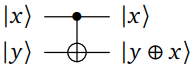
\includegraphics[scale=1]{./cnot}
\end{center}

\textbf{La porte SWAP} échange deux qubits d'entrée
\begin{center}
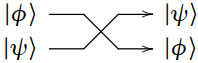
\includegraphics[scale=1]{./swap}
\end{center}

\textbf{La porte FANOUT} transforme un 1-qubit en 2-qubit. Dans un circuit quantique, cela permet d'augmenter le nombre de lignes quantiques
\begin{center}
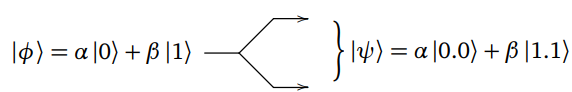
\includegraphics[scale=1]{./fanout}
\end{center}
\subsection{Les opérations sur les qubits}
\subsubsection{Addition sur 1-qubit}
Soient $\ket{\psi_1}=\alpha_1 \ket{0}+ \beta_1 \ket{1}   $ et $\ket{\psi_2}=\alpha_2 \ket{0}+ \beta_2 \ket{1}   $\\
On a $\ket{\psi_1} +  \ket{\psi_2}= (\alpha_1 + \alpha_2)\ket{0}+ (\beta_1 + \beta_2)\ket{1}   $

\subsubsection{Addition sur 2-qubit}

Soient $\ket{\psi_1}=\alpha_1 \ket{0.0}+ \beta_1 \ket{0.1}+ \delta_1\ket{1.0} + \lambda_1 \ket{1.1}  $ et$\ket{\psi_1}=\alpha_2 \ket{0.0}+ \beta_2 \ket{0.1}+ \delta_2\ket{1.0} + \lambda_2 \ket{1.1}  $\\
On a $\ket{\psi_1} +  \ket{\psi_2}= (\alpha_1 + \alpha_2)\ket{0.0}+ (\beta_1 + \beta_2)\ket{0.1} + (\delta_1 + \delta_2)\ket{1.0} + (\lambda_1 + \lambda_2)\ket{1.1} $

\subsubsection{Multiplication}

 Soit les qubits $\ket{i}$ et $\ket{j} $ la multiplication de deux 1-qubit donne 2-qubit\\
 $ \ket{i}\cdot \ket{j}=\ket{i\cdot j}  $


\subsection{Les n-qubits}
Un n-qubit est la superposition de $n$ états quantiques de base.\\
Soit $\ket{\psi} $ un n-qubit alors il s'écrit \\
$\ket{\psi}=\alpha_0 \ket{0 \cdots 0}+ \alpha_1 \ket{0 \cdots 1}+ \cdots +\alpha_{2^n -1} \ket{1 \cdots 1}  $\\
Exemple: 3-qubit\\
$\ket{\psi}=\alpha_0 \ket{0.0.0} + \alpha_1 \ket{0.0.1} + \alpha_2 \ket{0.1.0}+ \alpha_3 \ket{1.0.0} + \alpha_4 \ket{0.1.0} + \alpha_5 \ket{0.1.1}+ \alpha_6 \ket{1.1.0}+\alpha_7 \ket{1.1.1} $\\
On constate nous avons 8 termes pour 3-qubits pour un  état quantique alors qu'informatique classique travailler avec 3 bits revient à faire 8 entrées possibles d'où la puissance de la machine quantique.


\subsubsection{Mesure d'un n-qubit}
Soit $\ket{\psi}=\alpha_0 \ket{0 \cdots 0}+ \alpha_1 \ket{0 \cdots 1}+ \cdots +\alpha_{2^n -1} \ket{1 \cdots 1}  $ un n-qubits telle que \\
$\lVert \psi \rVert=\sqrt{{\mid \alpha_0 \mid}^2+ \cdots +{\mid \alpha_{2^n - 1} \mid}^2 }=1 $


\[  
mesure(\psi) \left \{
\begin{array}{ c  c }
0.0\cdots 0 \hspace{0.5cm} \text{avec une proba} \hspace{1.5cm} {\mid \alpha_0 \mid}^2\\
0.0\cdots 1 \hspace{0.5cm} \text{avec une proba} \hspace{1.5cm} {\mid \alpha_1 \mid}^2\\
\vdots \hspace{0.5cm} \cdots \\
1.1\cdots 1   \hspace{0.5cm} \text{avec une proba} \hspace{1.5cm} {\mid \alpha_{2^n -1} \mid}^2\\
  
\end{array}
\right.
\]
\subsubsection{Les portes à Trois entrées}
\textbf{Porte de Toffoli (CCNOT):} La porte de Toffoli est similaire à une porte CNOT mais avec trois lignes. Si les deux premiers qubits sont $\ket{1}$, alors on applique une porte \textbf{X} (c'est -à-dire NOT) au troisième qubit.\\ Voici l'action d'une porte de Toffoli lorsque $x,y,z  $  sont des bits 0 ou 1 (noter que $xy=1  $ si et seulement si $x=1 $ et $ y=1 $ et alors $ 1\bigoplus z = NOT(z) $)
\begin{center}
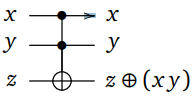
\includegraphics[scale=1]{./toffoli}
\end{center}
\subsection{Oracle}

Soit le groupe $ (\mathbb{Z}/n \mathbb{Z},+) $ correspond à l'ensemble des entiers modulo n représenté par \\ $\left\lbrace  0,1,\cdots,n-1 \right\rbrace $ pour $n=2  $ on a le groupe $ (\mathbb{Z}/2 \mathbb{Z}) $ qui est l'ensemble $\left\lbrace 0,1 \right\rbrace   $, muni de l'addition binaire notée  $ \oplus $ qui vérifie
$ 1 \oplus 1 =0   $, ce qui est cohérent car $1+1 \equiv 0 \mod 2  $.

\begin{definition}
Nous allons associer à une fonction $f$ un oracle. L’oracle d’une fonction $f$ est un circuit quantique dont on
explicite seulement l’entrée et la sortie (qui dépend de $f$ ). C’est une sorte de boîte noire, car nous n’avons
pas besoin de connaître les détails du circuit qui réalise un oracle.
\end{definition}
\textbf{Cas $ f: \mathbb{Z}/2\mathbb{Z} \rightarrow \mathbb{Z}/2\mathbb{Z} $}: la transformation effectuée par un oracle, lorsque les entrées sont des bits classiques $0 $ ou $1 $.\\
\begin{center}
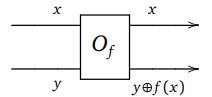
\includegraphics[scale=1]{./oracle1}
\end{center}
Il y a deux lignes pour l’entrée de l’oracle et deux lignes pour la sortie. La première sortie laisse la première
entrée inchangée. Pour la seconde sortie : si $x$ et $y$ sont $0$ ou $1$ alors la seconde sortie est $y \oplus  f (x)$; c’est
donc $y$ si $f (x) = 0$ et $ NON( y)$  si  $ f (x) = 1$ .\\
Ainsi l’oracle associé à f fournit une fonction

\[  
 \left.
\begin{array}{ c  c }
\mathbf{F}: \mathbb{Z}/2\mathbb{Z} \times \mathbb{Z}/2\mathbb{Z} \rightarrow \mathbb{Z}/2\mathbb{Z} \times \mathbb{Z}/2\mathbb{Z}\\
(x,y) \longmapsto (x,y \oplus f(x))

\end{array}
\right.
\]

Nous verrons plus tard comment cela définit naturellement une transformation quantique sur les 2-qubits.
Pour l’instant nous généralisons l’oracle au cas d’autres fonctions.\\
\textbf{Cas $ f: \mathbb{Z}/n\mathbb{Z} \rightarrow \mathbb{Z}/2\mathbb{Z} $}:\\

Cette situation correspondra à l’algorithme de Grover. On fixe $n \geq 2$ et on considère une fonction quelconque
$ f : \mathbb{Z}/n\mathbb{Z}\rightarrow \mathbb{Z}/2\mathbb{Z}$ que l’on peut aussi voir comme une fonction $ f : \left\lbrace 0, 1,\cdots , n- 1 \right\rbrace  \rightarrow \left\lbrace  0, 1\right\rbrace $.
La transformation de l’oracle, pour  $ x \in  \mathbb{Z}/n\mathbb{Z}  $ et $ y \in \mathbb{Z}/2\mathbb{Z} $, renvoie une nouvelle fois $x$ (élément de $ \mathbb{Z}/n\mathbb{Z} $)
et $y \oplus f (x)$  (élément de $ \mathbb{Z}/2\mathbb{Z} $)\\
On obtient ainsi :

\[  
 \left.
\begin{array}{ c  c }
\mathbf{F}: \mathbb{Z}/n\mathbb{Z} \times \mathbb{Z}/2\mathbb{Z} \rightarrow \mathbb{Z}/n \mathbb{Z} \times \mathbb{Z}/2\mathbb{Z}\\
(x,y) \longmapsto (x,y \oplus f(x))

\end{array}
\right.
\]

\paragraph{Exemple\\}


Fixons $ l \in \left\lbrace 0,\cdots, n-1 \right\rbrace $ un entier et $f : \mathbb{Z}/n\mathbb{Z} \rightarrow \mathbb{Z}/2\mathbb{Z} $ tel que $f (x) = 0$ pour tout $x$, sauf $f (l) = 1$.\\
Alors :

\begin{itemize}

\item[•] pour $x \neq $ et $y = 0$ on a $y \oplus f (x) = 0$,
\item[•] pour $x \neq $ et $y = 1$ on a $ y \oplus f (x) = 1$,
\item[•] pour $x = l $ et $y = 0 $ on a $y \oplus f (x) = 1$ ,
\item[•] pour $ x = l $ et $y = 1 $ on a $ y \oplus f (x) = 1 \oplus 1 = 0$
\end{itemize}
\textbf{Cas $ f:( \mathbb{Z}/n\mathbb{Z})^k \rightarrow \mathbb{Z}/2\mathbb{Z} $ \\}

Cette situation correspondra à l’algorithme de \textbf{Deutsch–Jozsa}.
On fixe $k \geq 1$ et on considère une fonction quelconque $f : \mathbb{Z}/n\mathbb{Z})^k \rightarrow \mathbb{Z}/2\mathbb{Z}$ que l'on peut aussi voir comme une fonction $ f:{\left\lbrace 0,1 \right\rbrace}^k \rightarrow \left\lbrace 0,1 \right\rbrace    $

 que l’on peut aussi voir comme
une fonction $ f:{ \left\lbrace 0,1 \right\rbrace}^k \rightarrow \left\lbrace 0,1\right\rbrace   $.\\
.
La transformation de l’oracle, pour $ x = (x_1
,\cdots , x_k
) \in {\mathbb{Z}/2\mathbb{Z}}^k$
et $ y \in  \mathbb{Z}/2\mathbb{Z} $ , renvoie $x = (x_1
, \cdots , x_k
)$
(élément de $(\mathbb{Z}/2\mathbb{Z})^k$
) et $ y \oplus f (x)$ (élément de $ \mathbb{Z}/2\mathbb{Z}$ )

\begin{center}
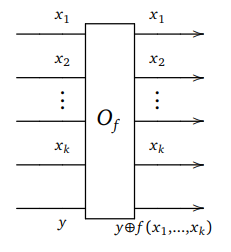
\includegraphics[scale=1]{./oracle2}

\end{center}
On obtient ainsi: 

\[  
 \left.
\begin{array}{ c  c }
\mathbf{F}: {(\mathbb{Z}/2\mathbb{Z})}^k \times \mathbb{Z}/2\mathbb{Z} \rightarrow {(\mathbb{Z}/2\mathbb{Z})}^k \times \mathbb{Z}/2\mathbb{Z}\\
(x_1,\cdots,x_k,y) \longmapsto (x_1,\cdots,x_k,y \oplus f(x_1,\cdots,x_k))

\end{array}
\right.
\]

\textbf{Exemple}: \\

On considère $ f : {(\mathbb{Z}/2\mathbb{Z})}^2 \rightarrow {(\mathbb{Z}/2\mathbb{Z})} $ définie par $ f(x,y)=x$ XOR $y $. Voici quelques exemples d’action de l’oracle:

\begin{center}
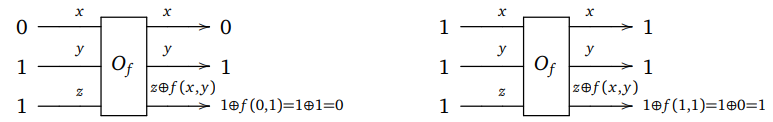
\includegraphics[scale=1]{./oracle3}
\end{center}

Autrement dit $\mathbf{F}(0, 1, 1) = (0, 1, 0)$ et $ \mathbf{F}(1, 1, 1) = (1, 1, 1)$

On pourrait généraliser l’oracle au cas d’une fonction $f : E \rightarrow E' $
 pour lequel l’oracle associé serait une
fonction $F : E \times  E'
 \rightarrow E \times  E' $
 défini par $F(x, y) = (x, y \oplus  f (x))$ où « $ \oplus $ » est une addition dans $E'$

\subsection{Transformation quantique}
Considérons  le cas d'une fonction $ f:{(\mathbb{Z} / 2\mathbb{Z})}^2  \rightarrow (\mathbb{Z}/2\mathbb{Z})  $. L'oracle fournit une fonction $\mathbf{F}:{(\mathbb{Z}/2\mathbb{Z})}^{k+1}  \rightarrow {(\mathbb{Z}/2\mathbb{Z})}^{k+1} $ en ayant considéré ${(\mathbb{Z}/2\mathbb{Z})}^{k} \times \mathbb{Z}/2\mathbb{Z} ={(\mathbb{Z}/2\mathbb{Z})}^{k+1}$. Voyons la transformation quantique associée sur les $(k+1)$-qubits.\\
Les $(k+1)$-qubits sont engendrés par la base canonique formée des $2^{k+1}$ qubits de base:
\begin{center}
$ \ket{0.0\cdots 0}\hspace{0.5 cm} \ket{0.0\cdots 1}\hspace{0.5 cm} \cdots \hspace{0.5 cm} \ket{1.1\cdots 1} $
\end{center}
La fonction $\mathbf{F} $ (définie sur des $(k+1) $-bits) s'étend naturellement en une fonction $\tilde{\mathbf{F}}$ sur les vecteurs de la base des $(k+1)$-qubits :



\[  
 \left.
\begin{array}{ c @{\overset{\tilde{\mathbf{F}}}{\mapsto}}  c }
\ket{e_0}=\ket{0.0\cdots 0}\hspace{0.8cm} & \hspace{0.5cm}\ket{\mathbf{F}(0,0,\cdots,1)}=\ket{f_0}\\
\ket{e_1}=\ket{0.0\cdots 1}\hspace{0.8cm} & \hspace{0.5cm}\ket{\mathbf{F}(0,0,\cdots,1)}=\ket{f_1}\\
\cdots \\
\ket{e_{2^{k+1}-1}}=\ket{1.1\cdots 1}\hspace{0.8cm} & \hspace{0.5cm}\ket{\mathbf{F}(1,1,\cdots,1)}=\ket{f_{2^{k+1}-1}}\\
\end{array}
\right.
\]
Maintenant que $\tilde{\mathbf{F}} $ est définie sur les vecteurs de la base par la relation $ \tilde{F}(\ket{e_i})=\ket{F(e_i)}=\ket{f_i}  $, elle s'étend par linéarité à tous les $(k+1) $-qubits.Ainsi on obtient
\begin{center}
$ \tilde{F}:\mathbb{C}^{2^{k+1}} \rightarrow \mathbb{C}^{2^{k+1}}  $
\end{center}

et pour un $(k+1)$-qubits 
\begin{center}
$ \ket{\psi}=\sum_{i=0}^{2^{k+1}-1}\alpha_i \ket{e_i} $ avec $\alpha_i \in \mathbb{C}  $, on obtient le $(k+1)$-qubit :
\end{center}
\begin{center}
$ \tilde{\mathbf{F}}(\ket{\psi})=\alpha_i \ket{f_i} $
\end{center}

Comme $F $ est bijective alors $\tilde{F} $ envoie l'ensemble des vecteurs de la base canonique sur ces mêmes vecteurs de la base canonique(autrement dit $\tilde{F} $ permute les vecteurs de la base).\\
\textbf{Notation}: On fixe un entier $ n \geq 1  $. Soit  $ 0 \leq k \leq 2^{n}-1$. Notons $ \underline{k} $ l'écriture binaire de l'entier $k$ sur $n$ bits. L'écriture entière $ \underline{k} $ désigne le n-qubit de la base canonique associée à l'écriture binaire $k$.\\
Exemple:Pour $n=1 $ il y' a seulement deux qubits de base $\ket{\underline{0}}=\ket{0} $ et $\ket{\underline{1}}=\ket{1} $ \\Pour $ n=2 $ $\ket{\underline{0}}=\ket{0.0} $ $\ket{\underline{1}}=\ket{0.1} $ ,$\ket{\underline{2}}=\ket{1.0} $,
$\ket{\underline{3}}=\ket{1.1} $

\subsubsection{La transformation de Hadamard}

On rappelle que la porte de Hadamard est défine pour les 1-qubits par la formule:


\begin{center}

$ H\ket{0}=\frac{1}{\sqrt{2}}(\ket{0}+ \ket{1}) $ et $ H\ket{1}=\frac{1}{\sqrt{2}}(\ket{0}- \ket{1}) $
\end{center}
La transformation de Hadamard d'un n-qubit $\ket{\psi} $ est l'application d'une porte de Hadamard sur chacun des 1-qubits le constituant.On note cette transformation $ \mathbf{H}^{\otimes n} $.\\ Le circuit est simplement composé de $n$ lignes, avec une porte de Hadamard par ligne (l'ordre de ces portes n'a pas d'importance).

\begin{center}
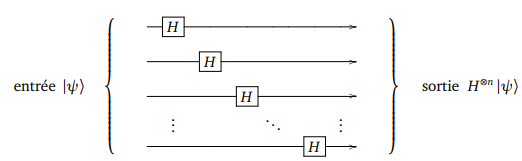
\includegraphics[scale=1]{./schadamard}
\end{center}

\textbf{Exemple}: pour n=2\\
$\ket{\underline{0}}=\ket{0.0} \overset{\mathbf{H}^{\otimes n}}{\rightarrow} \frac{1}{2} (\ket{0+1} \ket{0+1})=\frac{1}{2} (\ket{0.0}+ \ket{0.1}+\ket{1.0}+\ket{1.1}) = \frac{1}{2} (\ket{\underline{0}}+\ket{\underline{1}} + \ket{\underline{2}}+\ket{\underline{3}})$\\
$\ket{\underline{1}}=\ket{0.1} \overset{\mathbf{H}^{\otimes n}}{\rightarrow} \frac{1}{2} (\ket{0+1} \ket{0-1})=\frac{1}{2} (\ket{0.0}- \ket{0.1}+\ket{1.0}-\ket{1.1}) = \frac{1}{2} (\ket{\underline{0}}-\ket{\underline{1}} + \ket{\underline{2}}-\ket{\underline{3}})$
\subsubsection{Formule de la transformation de Hadamard}
Soit $n\geq 1$, en se basant de ce qui précède on a:\\
pour $ n=2    $, $H\ket{\underline{0}}=\frac{1}{2} (\ket{\underline{0}}+\ket{\underline{1}} + \ket{\underline{2}}+\ket{\underline{3}}) $\\ 
$H\ket{\underline{0}}=\frac{1}{\sqrt{2}^2} \sum_{l=0}^{2^2 -1} \ket{\underline{l}} $\\
D'une autre  manière avec  on a:

\begin{center}
$ \mathbf{H}\ket{\underline{0}}=\frac{1}{\sqrt{2^n}}\mathlarger \sum_{l=0}^{2^n -1} \ket{\underline{l}} $
\end{center} 

La formule générale est donnée par la proposition suivante:
\begin{proposition} Pour $ 0\leq k\leq 2^n-1  $, on a :\\
\begin{center}
$  \mathbf{H}^{\otimes n}\ket{\underline{k}} =\frac{1}{\sqrt{2^n}}\mathlarger \sum_{l=0}^{2^n -1} (-1)^{\underline{k}\odot \underline{l}} \ket{\underline{l}} $
\end{center}
\end{proposition}
\textbf{Notation}: Pour l'écriture binaire $ \underline{k}=k_1 . k_2 \cdots k_n $ et l'écriture binaire $ \underline{l}=l_1. l_2 \cdots l_n $(avec $k_i $,$l_i \in \left\lbrace 0,1 \right\rbrace  $)\\
$ \underline{k}\odot \underline{l}=k_1 l_1 \oplus k_2 l_2 \oplus k_n l_n \in \left\lbrace 0,1\right\rbrace    $.\\
C'est comme un produit scalaire modulo 2
\paragraph{Exemple :\\}
Soit $n=3 $ et $\ket{\underline{5}}=\ket{1.0.1} $,alors un calcul direct donne :\\
 
\[  
 \left.
\begin{array}{ c  c }
\mathbf{H}^{\oplus 3} \ket{\underline{5}}= \mathbf{H}^{\oplus 3} \ket{1.0.1}\\
 = \frac{1}{2\sqrt{2}}\ket{(0-1).(0+1).(0-1)}\\
 = \frac{1}{2\sqrt{2}}\left( \ket{(0.0.0)}-\ket{(0.0.1)}+\ket{(0.1.0)}-\ket{(0.1.1)}-\ket{(1.0.0)}+\ket{(1.0.1)}-\ket{(1.1.0)}+\ket{(1.1.1)}\right) \\
\end{array}
\right.
\]
Dans ce qui précéde nous avons vu les éléments de base de l'informatique quantique et qui forment les principaux constituants du circuit de l'algorithme de Grover.

\subsection{L'algorithme de Grover}
L'algoritme de Grover est basé sur la recherche d'un  élément sur une liste de taille $N $. Il est d'une complexité 
$\sqrt{N} $ et d'une probabilté $1-\frac{4}{N}$ de donner le bon élément. Parler d'un circuit de Grover revient à décrire, les entrées, l'oracle et la transformation de Grover et l'ensemble des portes quantiques qui le composent.


\subsubsection{Oracle de Grover}
On se place dans le cas où $N $ est une puissance de 2: $N=2^n $. On se rappelle que pour $0 \leq k \leq N-1  $, alors $ \underline{k}$ est l'écriture binaire de k sur n bits. Ainsi $\ket{k} $, pour 
$k=0,\cdots,2^{n}-1 $,désigne les n-qubits de la base canonique: $\ket{\underline{0}}=\ket{0.0\cdots0}  $,$ \ket{\underline{1}}=\ket{0.0\cdots 1} ,\cdots,\ket{2^n-1}=\ket{1.1\cdots 1}$.\\
Nous allons utiliser l'oracle $O_f  $ associé à la fonction $f$.Pour $ x \in \mathbb{Z}/N \mathbb{Z} $ et $ y \in \mathbb{Z}/2 \mathbb{Z}  $, l'oracle réalise une fonction $\mathbf{F}(x,y)=(x,y\oplus f(x))  $.On préfère écrire l'entier $x$ à l'aide de son écriture binaire $\underline{x}=x_1 . x_2 \cdots x_n  $, ce qui permet de récrire la fonction $\mathbf{F} $ sous la forme $ \mathbf{F}(x,y)=(x_1,\cdots,x_n,y\oplus f(x_1,\cdots,x_n))    $\cite{Arnaud}-p4.


\begin{center}
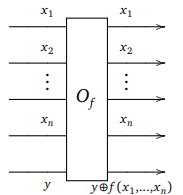
\includegraphics[scale=1]{./oracle_grover}
\end{center}
En appliquant $ \ket{\underline{x}}=\ket{\underline{0}}$ et posant $ y \oplus f(x_1,\cdots,x_n)=1  \Rightarrow y=1 $  \\
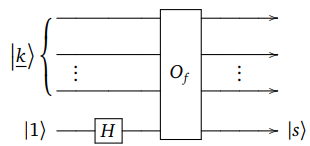
\includegraphics[scale=1]{./oracle_2}
L'entrée $\ket{1} $ est d'un porte de hadamard et de l'oracle  d'où la sortie
$\ket{s} =\frac{1}{\sqrt{2}}(\ket{0}-\ket{1})\oplus f(k)=(-1)^{f(k)}\frac{1}{\sqrt{2}}(\ket{0}-\ket{1})$


\[  
 \ket{s}= \left\lbrace 
\begin{array}{ c  c }
\frac{1}{\sqrt{2}}(\ket{0}-\ket{1})\hspace{0.5cm} \text{si} k \neq  k_0\\
 - \frac{1}{\sqrt{2}}(\ket{0}-\ket{1})\hspace{0.5cm} \text{si} k = k_0

\end{array}
\right.
\]
L'oracle nous permet de faire une remarque : le signe du terme au rang $k_0 $ est négatif "-" \\
Ainsi nous allons procéder à la détection du rang $k_0 $.\\ Mais celle-ci se fera par des transformations géométriques.
\subsubsection{Symétrie de l'oracle}
L'oracle transforme $\ket{k_0} $ en $-\ket{k_0} $ et laissant inchangé les $ k \neq k_0$. Soit $\ket{\phi}$ un n-qubit en isolant $k_0 $ on a

$ \ket{\phi}=\alpha \ket{\underline{k_0}}+ \sum_{ k \neq k_0}\alpha_k  \ket{\underline{k}}$\\
L'action de l'oracle $O_f $ sur $ \ket{\phi}$ est :$ \ket{\phi}=-\alpha \ket{\underline{k_0}}+ \sum_{ k \neq k_0}\alpha_k  \ket{\underline{k}}$
 
\begin{center}
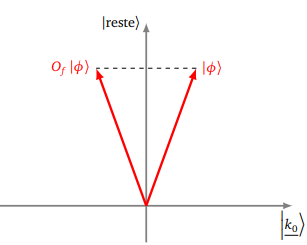
\includegraphics[scale=1]{./symetrie}
\end{center}

Ainsi $O_f \ket{\phi} $ est le symétrique de $\ket{\phi} $ par rapport à l'axe $\ket{reste} $ qui sont l'ensemble des termes autres que $\ket{k_0} $.\\
Nous allons définir cette symétrie axiale par récurrence induite par l'oracle\\

Soit $\mathbf{S}_0 $, la transformation définie sur les n-qubits de la base canonique par :


\[  
  \left\lbrace 
\begin{array}{ c @{\hspace{0.1cm}\overset{S_0}{\mapsto}\hspace{0.1cm}}  c }
\ket{\underline{0}}& \ket{\underline{0}}\\

\ket{\underline{k}}& -\ket{\underline{k}} \hspace{0.2cm} \text{si} \hspace{0.8cm} k\neq 0
\end{array}
\right.
\]
On voit c'est seulement le qubit $\ket{\underline{0}} $ qui ne change pas.
Par exemple $n=2 $ , on a $S_0 \ket{0.0}=\ket{0.0} $,$S_0 \ket{0.1}=-\ket{0.1} $,$S_0 \ket{1.0}=-\ket{1.0} $,$S_0 \ket{1.1}=-\ket{1.1} $.\\
Comme on étend $S_0 $ par linéarité à tous les n-qubits. \\
$ S_0(\alpha \ket{0.0}+ \beta \ket{0.1}+\gamma \ket{1.0}+\delta \ket{1.1})=
\alpha \ket{0.0}- \beta \ket{0.1}-\gamma \ket{1.0}-\delta \ket{1.1}  $
\begin{center}
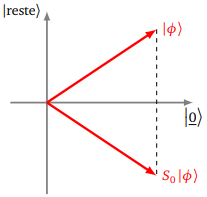
\includegraphics[scale=1]{./sym}
\end{center}

Lemme suivant donne l'expression algébrique de $S_0 $
\begin{lemme}


$ S_0=2\ket{\underline{0}}\bra{\underline{0}}- I $

 $I $ désigne l'application identité. Ainsi cette formule signifie que pour un qubit $\ket{\phi} $ on a:\\
 $S_0 \ket{\phi}=2 \ket{\underline{0}} \bra{\underline{0}}{\phi}-\ket{\phi} $\\
 L'écriture $\ket{\underline{0}}\braket{\underline{0}}{\phi} $ est bien qubit car $\braket{\underline{0}}{\phi} $ est un scalaire (i.e un nombre complexe)

\end{lemme}
Soit la transformation $S_{\psi} $ avec 
$\ket{\psi}$ un n-qubit de norme 1.
Nous allons montrer que \\ 
$ S_{\psi}=2\ket{\psi}\bra{\psi}- I $\\
Soit $\ket{\phi} $ un n-qubit quelconque on a $S_{\psi}\ket{\phi}=(2\ket{\psi}\bra{\psi}- I)\ket{\phi } $\\
$ S_{\psi}\ket{\phi}=2\ket{\psi}\braket{\psi}{\phi}-\ket{\phi} $\\
Cette transformation vérifie :

\[  
  \left\lbrace 
\begin{array}{ c @{\hspace{0.1cm}\overset{S_{\psi}}{\mapsto}\hspace{0.1cm}}  c }
\ket{\psi}& \ket{\psi}\\

\ket{\phi}& -\ket{\phi} \hspace{0.2cm} \text{si} \ket{\phi} \hspace{0.5cm}\text{est orthogonal à} \hspace{0.5cm} \ket{\psi}
\end{array}
\right.
\]
\begin{center}
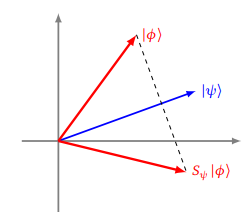
\includegraphics[scale=1]{./symphi}
\end{center}

Géométriquement $S_{\psi} $ est une symétrie par rapport à l'axe dirigé par $\ket{\psi} $. 
\subsubsection{Transformation $\mathit{S}_{\psi_H} $}

Notons  $\ket{\psi_H} $ le n-qubit formé par la somme de tous les qubits de la base canonique :


\begin{center}
$  \ket{\psi_H}=\frac{1}{\sqrt{2^n}}\sum_{k=0}^{2^n-1}\ket{\underline{k}} $
\end{center}
ce qubit $\ket{\psi_H} $ est aussi l'image du qubit $\ket{0...0} $ par transformation de Hadamard:

\begin{center}
$  \ket{\psi_H}=\frac{1}{\sqrt{2^n}}\sum_{k=0}^{2^n-1}\ket{\underline{0}} $
\end{center}

\begin{proposition}
La transformation de $\ket{\psi_H} $ est  définie par l'une des caractérisations équivalentes suivantes:
\begin{itemize}
\item[(i)] $ \mathit{S}_{\psi_H}=2\ket{\psi_H}\bra{\psi_H}-I $, c'est-à-dire $ \mathit{S}_{\psi_H} \ket{\phi}=2\ket{\psi_H}\braket{\psi_H}{\phi}-\ket{\phi} $ pour tout qubit $\ket{\phi} $

\item[(ii)] $ 
  \left\lbrace 
\begin{array}{ c @{\hspace{0.1cm}\overset{S_{\psi_H}}{\longmapsto}\hspace{0.1cm}}  c }
\ket{\psi_H}& \ket{\psi_H}\\

\ket{\phi}& -\ket{\phi} \hspace{0.2cm} \text{si \hspace{0.2cm}} \ket{\phi} \hspace{0.5cm}\text{est orthogonal à} \hspace{0.5cm} \ket{\psi_H}
\end{array}
\right.
$
\item[(iii)] $ \mathit{S}_{\psi_H}=\mathit{H}^{\otimes n}\cdot \mathit{S}_0 \cdot \mathit{H}^{\otimes n} $

\item[(iv)] $\mathit{S}_{\psi_H} $ a pour matrice 
\begin{center}
$\frac{2}{2^n}\mathit{U}-I $ où $ \mathit{U}=\begin{pmatrix}
1 & 1      & \cdots & 1\\
1 & \ddots &        & 1\\
\vdots &    &    \ddots    & \vdots\\
1      &\cdots   &1&1
\end{pmatrix} \in \mathbf{M}_{2^n}  $
\end{center}



\end{itemize}

\begin{center}
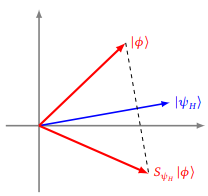
\includegraphics[scale=1]{./transpo2}
\end{center}

\end{proposition}

Géométriquement on voit que la transformation $ \mathit{S}_{\psi_H}  $ d'un n-qubit $\ket{\phi} $ est le symétrique de  $\ket{\phi} $ par rapport à l'axe de $\ket{\psi_H}  $

\subsection{Transformation de Grover}
La transformation de Grover est l'application \cite{Arnaud}p9
\begin{center}
$\mathit{G}=\mathit{S}_{\psi_H}\circ \mathit{O}_f$

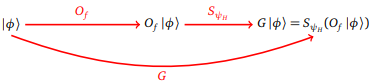
\includegraphics[scale=1]{./trans_grover}
\end{center}

Essayons d'expliquer cette transformation.\\ Soit le qubit $\ket{\psi_H}=\frac{1}{\sqrt{2^n}} \sum_{k=0}^{2^n-1}\ket{\underline{k}} $ obtenu comme la somme de tous les qubits de base isolant le terme de rang $ k_0$
on a: 
\begin{center}
$ \ket{\psi_H}=\frac{1}{\sqrt{N}}\ket{\underline{k_0}}+\frac{1}{\sqrt{N}} \sum_{k\neq k_0}^{N-2}\ket{\underline{k}} $ avec $N=2^n $\\
$ \ket{\psi_H}=\frac{1}{\sqrt{N}}\ket{\underline{k_0}}+\sqrt{N-1} \times \frac{1}{\sqrt{N-1}} \frac{1}{\sqrt{N}} \sum_{k\neq k_0}^{N-2}\ket{\underline{k}} $ \\
$ \ket{\psi_H}=\frac{1}{\sqrt{N}}\ket{\underline{k_0}}+\frac{\sqrt{N-1}}{\sqrt{N}} \times \frac{1}{\sqrt{N-1}}  \sum_{k\neq k_0}^{N-2}\ket{\underline{k}} $ \\
$ \ket{\psi_H}=\frac{1}{\sqrt{N}}\ket{\underline{k_0}}+\sqrt{\frac{N-1}{N}}  \frac{1}{\sqrt{N-1}}  \sum_{k\neq k_0}^{N-2}\ket{\underline{k}} $ \\


\end{center}

En posant $\ket{\mathcal{X}}=\frac{1}{\sqrt{N-1}}  \sum_{k\neq k_0}^{N-2}\ket{\underline{k}} $ on obtient $ \ket{\psi_H}=\frac{1}{\sqrt{N}}\ket{\underline{k_0}}+\sqrt{\frac{N-1}{N}}  \ket{\mathcal{X}} $ \\
Avec une écriture trigonométrique :
\begin{center}
$ \ket{\psi_H}=\cos{(\frac{\theta}{2})} \ket{\mathcal{X}}+\sin{(\frac{\theta}{2})} \ket{\underline{k_0}} $ où $\frac{\theta}{2} $ est l'angle entre $\ket{\mathcal{X}} $ et $\ket{\psi_H}  $

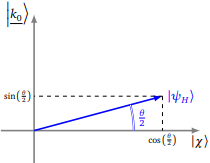
\includegraphics[scale=1.2]{./angle_g}\\
\end{center}
L'angle $\frac{\theta}{2} $ est défini par: 
\begin{center}
$ \cos{(\frac{\theta}{2})}=\sqrt{\frac{N-1}{N}}$ et $\sin{(\frac{\theta}{2})}=\frac{1}{\sqrt{N}} $
\end{center}
La proposition suivante donne une définition de la transformation grover
\begin{proposition}
La transformation de Grover est une rotation d'angle $\theta $ (centrée à l'origine).\cite{Arnaud}p9
\begin{center}
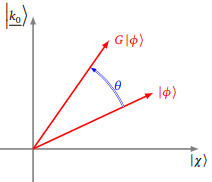
\includegraphics[scale=1]{./grover_2}
\end{center}
\end{proposition}

\paragraph{Démonstration :} Un résultat géométrique dit que la composition de deux symétries axiales est une rotation d'angle $\theta $ de cette rotation étant le double de l'angle entre les axes. 
Ici \textbf{G} est la composition de deux symétries:
\begin{itemize}
\item[•] la symétrie $\mathit{O}_f $ d'axe $\ket{\mathcal{X}} $,
\item[•] la symétrie $\mathit{S}_{\phi_H} $ d'axe $\ket{\psi_H} $
\item[•] l'angle entre $\ket{\mathcal{X}} $ et $\ket{\psi_H} $ est $\frac{\theta}{2} $
\end{itemize}
Ainsi $\mathbf{G}=\mathit{S}_{\psi_H}\circ \mathit{O}_f $ est la rotation d'angle $\theta $ (centrée à l'origine).
\begin{center}
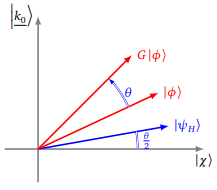
\includegraphics[scale=1.2]{./grover_3}
\end{center}

\subsubsection{Idée de l'algorithme }
Le but de l'algorithme de Grover est de déterminer le rang $k_0$. Ce rang est repérable après l'application de l'oracle $\mathit{O}_f$. \cite{Arnaud}-p12
\begin{center}
$\ket{\psi_H}=\frac{1}{\sqrt{2^n}}\sum_{k=0}^{2^n-1}\ket{\underline{k}}=\sqrt{\frac{N-1}{N}}  \ket{\mathcal{X}} +\frac{1}{\sqrt{N}}\ket{\underline{k_0}}  $
\end{center}
L'action de l'oracle donne $\mathit{O}_f \ket{\psi_H}=\sqrt{\frac{N-1}{N}}  \ket{\mathcal{X}}-\frac{1}{\sqrt{N}}\ket{\underline{k_0}}  $. Sur ce, nous avons les étapes suivantes:

\begin{itemize}
\item[•] La transformation de Hadamard envoie l'état initial $\ket{0.0...0} $ sur $\ket{\psi_H} $.
\item[•] On part du qubit $\psi_H $ qui est la superposition de tous les qubits de base
\item[•] Ce qubit forme un angle $\frac{\theta}{2} $ avec l'axe $\ket{\mathcal{X}} $.(L'angle $\frac{\theta}{2} $ est petit car $N=2^n $ est grand)
\item[•]La transformation de Grover est une rotation d'angle $\theta $ et conduit donc au qubit $G\ket{\psi_H}$ forme un angle $\frac{\theta}{2}+\theta $ avec l'axe $\ket{\mathcal{X}} $.
\item[•] On itère la transformation de Grover jusqu'à obtenir un qubit $G^{l}\ket{\psi_H} $ qui forme un angle d'environ $\frac{\pi}{2} $ avec l'axe $ \ket{\mathcal{X}}  $. (Ce nombre d'itérations $l$ est environ $\frac{\pi}{2 \theta} $)
\item[•] Le qubit $G^{l}\ket{\psi_H} $ obtenu est proche de $\ket{\underline{k_0}} $

\item[•] La mesure de ce qubit conduit très probablement à $\underline{k_0} $(avec une probabilité d'erreur très petite,d'ordre $ \frac{4}{N}$)

\end{itemize}

\subsubsection{Portes quantiques}
La transformation de Grover est la composition de l'oracle $\mathit{O}_f $ et de la transformation $\mathit{S}_{\psi_H} $. On a déjà vu le circuit quantique de l'oracle.\\

\begin{itemize}
\item[•] la porte \textbf{Z} est la porte principalement utilisée déjà vue

\item[•] \textbf{Porte CZ}.est composée d'un contrôleur et d'une porte \textbf{Z} fonctionne comme une porte \textbf{CNOT}: si l'entrée de la première ligne est $\ket{0} $, alors la seconde ligne est inchangée, par contre si l'entrée de la première ligne est $\ket{1} $, alors on fait agir une porte \textbf{Z} sur la seconde ligne.


\begin{center}
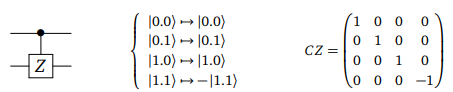
\includegraphics[scale=1.3]{./cz}
\end{center}

\end{itemize}

\subsubsection{Circuit quantique}

\paragraph{Circuit pour $ \mathit{S}_0$} Voici un circuit qui permet de réaliser la transformation $\mathit{S}_0$, dans le cas des 2-qubits. Noter bien que la partie droite du circuit est une porte \textbf{CZ}.
\begin{center}
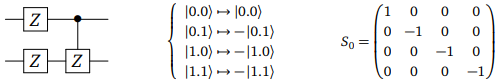
\includegraphics[scale=1.3]{./circuit_so}
\end{center}
\paragraph{Circuit pour $\mathit{S}_{\psi_H} $} On sait que $\mathit{S}_{\psi_H}=\mathbf{H}^{\otimes n}\cdot \mathit{S}_0 \cdot \mathbf{H}^{\otimes n} $, il suffit juste d'appliquer la transformation de Hadamard avant et après le circuit $ \mathit{S}_0$

\begin{center}
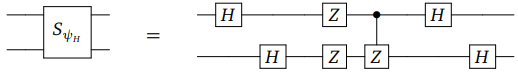
\includegraphics[scale=1.3]{./circuit_sw}
\end{center}
\subsection{Etapes de l'algorithme de Grover}

\subsubsection{Circuit}
On note \textbf{G} la transformation de Grover, elle prend en entrée un $(n+1)-$qubit, et est formée par la porte $\mathit{O}_f $ de l'oracle, suivie d'une porte associée à la transformation $\mathit{S}_{\psi_H}$. On représente cette porte \textbf{G} avec 2 lignes seulement, la première ligne correspond à un n-qubit(ligne symbolisée avec / ),la seconde à un $1-$qubit.

\begin{center}
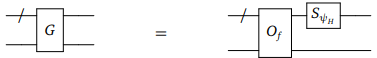
\includegraphics[scale=1.3]{./circuit_f}
\end{center}
Voici le circuit de l'algorithme de Grover.
\begin{center}
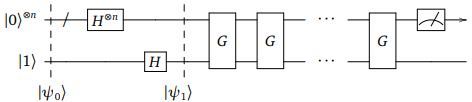
\includegraphics[scale=1.3]{./circuit_final}
\end{center}

La porte \textbf{G} est itérée $l$ fois avec $l \approx \frac{\pi}{4}\sqrt{N} $ où $\mathit{N}=2^n $. La complexité de l'algorithme est d'ordre $l$, donc d'ordre $\mathit{O}(\sqrt{N}) $. La mesure finale est la mesure d'un $n-$qubit(et correspond donc à n mesures de $1-$qubits). Le circuit renvoie donc un n-bit classique $\underline{k} $ avec $ 0\leq k < 2^n $. Nous allons justifier que cet entier est très probablement le rang $k_0 $ cherché.\cite{Arnaud}-14
\subsubsection{Données}

Soit $n \geq 1 $ et $ \mathit{N}=2^n $. Supposons donné un entier $k_0 $ vérifiant $0\leq k_0 \leq \mathit{N} $. On considère la fonction $ f:\mathbb{Z}/N\mathbb{Z}\longrightarrow \mathbb{Z}/2\mathbb{Z} $, avec $f(k_0)=1 $ et $f(k)=0 $ pour tout $ k \neq k_0 $
\subsubsection{Initialisation et transformation de Hadamard}

Le circuit quantique est initialisé par $(n+1)-$qubit \cite{Arnaud}
\begin{center}
$ \ket{\psi}=\ket{0...0}\cdot \ket{1}=\ket{\underline{0}}\cdot \ket{1} $
\end{center}
Ensuite on applique la transformation de Hadamard pour obtenir le qubit

$ 
  \left.
\begin{array}{ c @{=}  c }

\ket{\psi_1} & \mathbf{H}^{\otimes n +1} \ket{\psi_0}\\
& \mathbf{H}^{\otimes n}\ket{\underline{0}}\cdot \mathbf{H}\ket{1}\\
& \frac{1}{\sqrt{2^n}}\sum_{k=0}^{2^n-1}\ket{\underline{k}}\cdot \frac{1}{\sqrt{2}}(\ket{0}-\ket{1})\\
& \ket{\psi_H}\cdot \frac{1}{\sqrt{2}}(\ket{0}-\ket{1})\\

\end{array}
\right.
$

Dans la suite on oublie le dernier qubit et on s'intéresse seulement au n-qubit formé par les n premières lignes.\\
Dans $\ket{\psi_H}$ distinguons la qubit de base $\ket{k_0} $:

\begin{center}
$\ket{\psi_H}=\frac{1}{\sqrt{2^n}}\sum_{k=0}^{2^n-1}\ket{\underline{k}}=\sqrt{\frac{N-1}{N}}  \ket{\mathcal{X}} +\frac{1}{\sqrt{N}}\ket{\underline{k_0}}  $

\end{center}

que l'on récrit sous forme trigonométrique:
\begin{center}
$\ket{\psi_H}=\cos{(\frac{\theta}{2})}\ket{\mathcal{X}} + \sin{(\frac{\theta}{2})}\ket{\underline{k_0}} $
\end{center}

où $\frac{\theta}{2} $ est l'angle entre
$\ket{\mathcal{X}} $ et $\ket{\psi_H} $, également défini par la relation $\sin{\frac{\theta}{2}}=\frac{1}{\sqrt{N}} $


\begin{center}
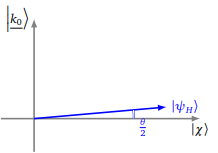
\includegraphics[scale=1.2]{./etape}
\end{center}

\subsubsection{Itérations de la transformation de Grover}
la transformation de Grover $\mathit{G}=\mathit{S}_{\psi_H}\circ \mathit{O}_f   $, est une rotation d'angle $\theta $.Donc après $l$ itérations on obtient le n-qubit.
\begin{center}
$ \mathit{G}^{l}\ket{\psi_H}= \cos{(\theta_l)}\ket{\mathcal{X}}+ \sin{(\theta_l)}\ket{\underline{k_0}} $ avec $ \theta_l=\frac{\theta}{2}+ l \theta $.
\end{center}
On veut $ \theta_l \approx \frac{\pi}{2} $, c'est-à-dire $\frac{\theta}{2}+ l \theta \approx \frac{\pi}{2}  $. Ainsi $l$ est défini comme l'entier le plus proche de $\frac{\pi}{2 \theta}-\frac{1}{2} $.
\begin{center}
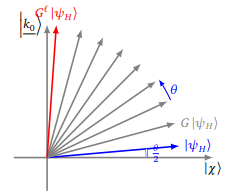
\includegraphics[scale=1.2]{./iteration}
\end{center}

Donnons une approximation du nombre $l$ d'itérations nécessaires. Pour cela nous considérons que $N=2^n $ est grand, et donc $\theta $ est petit. Comme $\sin{(\frac{\theta}{2})}=\frac{1}{\sqrt{N}}  $ alors $\frac{\theta}{2} \approx \frac{1}{\sqrt{N}}$ (car pour x proche de 0, $\sin{(x)}\approx x $). On veut $ l \theta \approx \frac{\pi}{2}  $
 donc $ l \approx \frac{\pi}{2 \theta} $
et ainsi 
\begin{center}
$ l \approx \frac{\pi}{4}\sqrt{N} $.
\end{center}

\subsubsection{Mesure}

Après ces $l$ itérations nous avons $\theta_l \approx \frac{\pi}{2} $, donc 
\begin{center}
$\mathit{G}^{l}\ket{\psi_H}=\cos{(\theta_l)}\ket{\mathcal{X}}+ \sin{(\theta_l)}\ket{\underline{k_0}}\approx \ket{\underline{k_0}} $.
\end{center}
La mesure de ce n-qubit conduit donc probablement au n-bit $\underline{k_0} $
et permet alors d'identifier le rang $k_0 $. 
\subsubsection{Probabilité de Grover}
\begin{proposition}
L'algorithme de Grover renvoie le rang correct $k_0 $ avec une probabilité supérieure à $1-\frac{4}{N} $.\cite{Arnaud}-p16
\end{proposition}


\paragraph{Démonstration\\}
\begin{itemize}
\item[•] Le qubit final obtenu par l'algorithme de Grover est 
\begin{center}
$\mathit{G}^{l}\ket{\psi_H}=\cos{(\theta_l)}\ket{\mathcal{X}}+ \sin{(\theta_l)}\ket{\underline{k_0}} $
\end{center}
Donc, lors de la mesure, la probabilté d'obtenir la bonne réponse $\underline{k_0} $ est $p= {\mid \sin{(\theta_l)}\mid}^2 $.
\item[•]  Nous savons que la transformation de Grover G est une rotation d’angle $\theta $ et nous avons itéré cette
transformation $ l$ fois de façon à construire un angle $ \theta_l = \frac{\theta}{2}+ l \theta $ le plus proche possible de l’angle $\frac{\pi}{2} $.
Ainsi l’angle $\theta_l$ est dans un intervalle d’amplitude $\theta $ centré en $ \frac{\pi}{2} $

\begin{center}
$ \frac{\pi}{2}-\frac{\theta}{2}< \theta \leq \frac{\pi}{2} \frac{\theta}{2}$
\end{center}

\item[•] Ainsi $\sin{(\theta_l)}\geq \sin{(\frac{\pi}{2}-\frac{\theta}{2})} $
(voir la figure ci-dessous)
\begin{center}
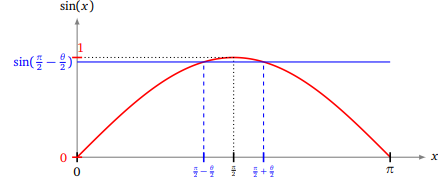
\includegraphics[scale=1.3]{./phase}
\end{center}
Donc: 
\begin{center}
$ \sin{(\theta_l)}\geq \sin{(\frac{\pi}{2}-\frac{\theta}{2})}=\cos{(\frac{\theta}{2})}\geq 1-\frac{1}{2}{(\frac{\theta}{2})}^2 $
\end{center}
.
Pour la dernière inégalité on connait le développement limité $\cos{(x)} \approx 1-\frac{x^{2}}{2}  $(pour x proche de 0) mais on a en plus l'inégalité $\cos{(x)}\geq 1-\frac{{x^2}}{2}   $(figure de gauche ci-dessous).
\begin{center}
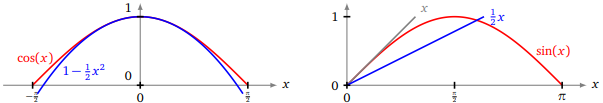
\includegraphics[scale=1.2]{./phase_2}

\item[•] L'angle $\theta $ est défini avec la relation $\sin{(\frac{\theta}{2})}=\frac{1}{\sqrt{N}} $. On sait, pour x proche de 0, on a $ \sin{(x)}\approx x $, mais on a en plus l'inégalité $\sin{(x)}\geq \frac{x}{2} $ (voir figure de droite ci-dessous). Ainsi, comme $\sin{(\frac{\theta}{2})}=\frac{1}{\sqrt{N}} $, alors $\frac{1}{\sqrt{N}}\geq \frac{\theta}{4}  $ donc $\frac{4}{N} \geq {(\frac{\theta}{2})}^2 $ et alors en reprenant les inégalités ci-dessus:\\

\begin{center}
$ \sin{(\frac{\theta_l}{2})}\geq 1-\frac{1}{2}{(\frac{\theta}{2})}^2 \geq 1- \frac{2}{N} $
\end{center}
Enfin on a $ {(1-x)}^2=1-2x+x^2 \geq 1-2x$ quel que soit x, donc
\\
\begin{center}
$ p=\mid \sin{(\theta_l)}^2 \geq {\left(1-\frac{2}{N} \right)}^2  \mid \geq 1-\frac{4}{N} $. \cite{Arnaud}-p17
\end{center}



\end{center}



\end{itemize}


\section{Les outils mathématiques des ISD}
\subsection{Le coefficient binomial et la fonction d'entropie}
\begin{definition} On définit la fonction d'entropie binaire par:

\[
\left.
\begin{array}{c  c}
   [-1 , 1] \longrightarrow ] 0,\frac{1}{2}]\\
    f \longmapsto  -(1-x)\log_2(1-x)-x\log_2(x)

\end{array}
\right.
\]


\end{definition}
\begin{theorem} Si H désigne la fonction d’entropie de Shannon, on a :{\Large $\frac{2^{nH(\frac{t}{n})}}{n+t}\leq{{n}\choose{t}}\leq 2^{nH(\frac{t}{n})}$}\\
Nous écrirons pour cela {\Large $  {n \choose t }\approx 2^{nH(\frac{t}{n})}$}.\cite{Ghazal}

\end{theorem}

\subsection{Codes poinçonnés}
\begin{definition} Étant donné un code C de matrice génératrice $ \mathbf{G}$ et de paramètres $[n, k]$ , le poinçonnage consiste à supprimer des colonnes de la matrice génératrice.\cite{Ghazal}-p1

\end{definition}
Soit $\mathit{I}$ un ensemble d’indice, $ \mid \mathit{I} \mid = i$. On note $\mathit{C}_I$ le code poinçonné dont la
matrice génératrice $\mathit{G}_I $ est la matrice de $\mathit{G}$ dont on a enlevé les colonnes indicées
par $ \mathit{I}$. Alors $\mathit{C}_I$ est de paramètres $[n-i, k]$. On notera $\mathit{H}_I$ la matrice de parité
de $\mathit{C}_I$ .
\begin{theorem} Soit $m$ un message de longueur $n$ et $m_I := m|I$. $\mid \mathit{I} \mid = i$. Soit $c_I = m_I \mathit{G}_I$ . Alors s’il y a une sous-matrice carrée inversible de $G_I$ , alors il est possible de dériver $c := mG$ de manière unique à partir de $c_I$ .\cite{Ghazal}

\end{theorem}
\textbf{Démonstration} On supposera pour simplifier que l’on a mis $G_I$ est sous forme systématique.\\
On suppose aussi que $i = 1$ et que $\mathit{I} = {n}$.
Alors $G$ s’écrit (à des permutations de colonnes et d’opérations de pivot de Gauss près) $(G_I |g_n)$, plus précisément :\\
\begin{center}

$\begin{bmatrix}
1 & \cdots & 0& | & \cdots& \cdots &\cdots&|g_{1,n}\\
\cdots & \cdots & \cdots& | & \cdots& \cdots &\cdots&|\cdots\\
0 & \cdots & 1& | & \cdots& \cdots &\cdots&|g_{n,k}
\end{bmatrix}$ 

\end{center}

Par conséquent si l’on écrit $m = (m_1, ..., m_n)$, $m_I = (m_1, \cdots, m_{n-1})$, $cI =(c_{I_1}, ..., c_{I_k})$, $c$ s’écrit $c = (c_{I_1} + g_{n,1mn},\cdots, c_{I_k} + g_{n,k}m_n)$.
Il suffit donc de connaître mn et la colonne gn de la matrice pour pouvoir calculer
$c$ à partir de $c_I$ .\\
Ce résultat se généralise facilement au cas où $i>2$, il faudrait alors connaître
les $(m_j)_{j \in I }$ et les colonnes $(g_j )_{j\in I}$ 

\begin{theorem}Soit le code $\mathit{C}$ ayant pour matrice génératrice $G = [Id|A]$ et donc
pour matrice de parité $H = [-A^T|Id]$ et soit $C_I$ le code obtenu en poinçonnant
les $i < k$ dernières de $G$, alors une matrice de parité $H_I$ de $C_I$ est donnée par la sous-matrice $(n-i)\times (n-k-i)$ "en haut à gauche" de $H$.\cite{Ghazal}\\


\end{theorem}

Illustration de ce théorème:
\begin{center}
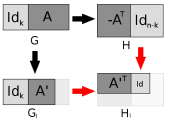
\includegraphics[scale=1.3]{./matrice}
\end{center}
\textbf{Démonstration}: On peut écrire $G = [Id_k|A] = [Id_k|A_1|A_2]$ où $A_1 \in M_{k,n-k-i}(\mathbb{F}_2)$
et $A_2 \in M_{k,i}(\mathbb{F}_2)$ correspond à la partie qui sera poinçonnée.\\
Alors, d’un côté $H = [-A^T|Id_{n-k}]$ avec $A^T =\begin{bmatrix}
A_1^T\\
  \vspace{0.1cm}\\
A_2^T

\end{bmatrix}$ donc au final, $H$ s’écrit de manière plus détaillée :

$\begin{bmatrix}
-A_1^T & Id_{n-k-i} & 0_{n-k-i,n-i}\\
A_2^T  & 0_{i,n-k-i} & Id_i

\end{bmatrix}$ 

D’un autre côté,$G_I = [Id_k|A_1]\in M_{k,n-i}(\mathbb{F}_2)$  donc $H_I = [A_1^T|Id_{n-k-i}]$, ce qui correspond à la sous-matrice de taille $(n-i)\times(n-k-i)$ "en haut à gauche"
de $H$.
\subsection{Dénombrement}
\begin{theorem}
Soit $\mathit{C}$ un code linéaire de paramètres $[n, k]$. Alors pour un syndrome $s \neq 0$ donné, le nombre moyen de mots $e \notin \mathit{C} $ de poids $p$  ayant
 pour syndrome $s$ est $\hspace{0.2cm}$ {\Large $ \frac{{n\choose p}}{2^{n-k}}$}.
\end{theorem}

\paragraph{Démontration}: admis \cite{Ghazal}-p3
\subsection{Distance de Gilbert-Varshamov}


\begin{theorem}
Soit $\mathit{C}$ un code linéaire de paramètres $[n, k]$. Soit $a_i$ le nombre moyen de mots de poids $i$ dans $\mathit{C}$. Alors :
\begin{enumerate}
\item $ \mathbb{E}(a_i)=1$ ssi $H(\frac{i}{n})=1-R \Leftrightarrow \frac{i}{n}=H^{-1}(1-R)$.\hspace{0.2cm} On appelle cette valeur
de i distance de Gilbert-Varshamov et on note cette fraction $d_{GV}:=H^{-1}(1-R)$.\cite{Ghazal}-p4
\item Plus généralement, le graphique suivant montre l’évolution du rapport $\log_2\left( \frac{\mathbb{E}(a_i)}{n} \right)$ en fonction de $\frac{i}{n}$:
\end{enumerate}
\end{theorem}
\begin{center}
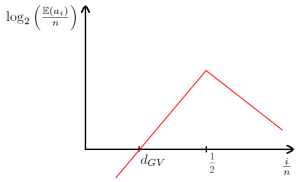
\includegraphics[scale=1.2]{./graphesperance}
\end{center}
\paragraph{Démonstration}: On a $a_i=\sum_{x,w_H(x)=i}\mathbf{1}_{x\in \mathit{C}}$\\
Par conséquent :\\
\begin{center}
\[
\left.
\begin{array}{c @{=} c}

     \mathbb{E}(a_i) & \sum_{x,w_H(x)=i}\mathbf{1}_{x\in \mathit{C}}    \\
      &\sum_{x,w_H(x)=i}\mathbb{P}(x \in \mathit{C})   \\
      & \sum_{x,w_H(x)=i}\frac{1}{2^{n-k}} \\
      & \frac{{n\choose t}}{2^{n-k}}   \\
       & \approx 2^{nH(\frac{i}{n})-(n-k)} \\
   &   2^{n(H(\frac{i}{n})-1+R)} 
    
\end{array}
\right.
\]






\end{center}
On pose $f(x)=H(x)-1+R$, on a alors $f(\frac{i}{n})=\log_2\left(\frac{\mathbb{E}(a_i)}{n} \right)$ et :
\begin{enumerate}
\item $f(x)=0 \Leftrightarrow x= H^{-1}(1-R)$ donc $\mathbb{E}(a_i)=1$ ssi $\frac{i}{n}=d_{GV}$
\item $ \max_{x\in \left\lbrace 0,1 \right\rbrace } f(x)=R $ pour l'argument $x=\frac{1}{2} $.
\end{enumerate}

\subsection{Combinatoire et probabilités}
\subsubsection{Combinatoire}
\begin{theorem} Soient $\mathit{S}$ un ensemble, $\mathit{M}$ un ensemble de données, $f : \mathit{S} \rightarrow  \mathit{M}$
une fonction aléatoire ou pseudo-aléatoire. On considère $m \in M$, $P_m : \mathit{S}\rightarrow  \left\lbrace 0, 1\right\rbrace  $ tel que $P_m(s) = 1 $ si $f(s) = m$ et $P_m(s) = 0$ sinon. Alors le nombre moyen d’éléments $s$ de $\mathit{S}$ tels que $P_m(s) = 1$ est $\frac{\mid S \mid }{\mid M \mid}$.\cite{Ghazal}
\end{theorem}
\paragraph{Démonstratin}: On numérote les éléments de $S$ et on définit pour $s_i$
, le $i^{ème}$ éléments, la variable aléatoire suivante :\\
$X_{i}=P_{m}(s_i)  $\\
Comme $f$ est aléatoire ou pseudo-aléatoire, on a $\mathbb{P}(X_i=1)=M^{-1}$ pour tout $i$.La variable $ X:=\sum_{i}X_i$ donne alors le nombre d'éléments de $ \mathit{S}$ tels que $P_{m}(s)=1 $. On calcule $\mathbb{E}(X)$:
\begin{center}
$ \mathbb{E}(X)=\sum_{i}\mathbb{E}(X_i)=\mid \mathit{S} \mid\mathbb{P}(X_i=1)=\frac{\mid S \mid}{\mid M \mid}$
\end{center}
\begin{theorem}
Soient $S_1$ et $S_2$ des ensembles, $ M $ un ensemble de données,$ f_1 : S_1 \rightarrow M $ et $ f_2 : S_2 \rightarrow M  $ des fonctions aléatoires ou pseudo-aléatoires. Alors la probabilité de collision des valeurs de $f_1$ et $ f_2$ est $\frac{\mid S_1 \mid \mid S_2 \mid}{\mid M \mid} $.\cite{Ghazal}
\end{theorem}

\paragraph{Démonstration}: On considère le produit cartésien $S = S_1 \times S_2$ et on numérote ses  $\mid S_1\mid \mid S_2\mid $ éléments. On définit pour son $i{ème}$ élément $(x, y)_i$
la variable aléatoire suivante :\\
$X_i=1$ si $f_1(x)=f_2(y)$,$X_i=0$ sinon.Comme $f_1$ et $f_2$ sont aléatoires ou pseudo-aléatoires, on a $\mathbb{P}(X_i=1)=M^{-1}$ pour tout $i$. La variable aléatoire $X:=\sum_{i}X_i$ donne alors le nombre d'éléments $(x,y)$ de $\mathit{S}$ tels que $f_1(x)=f_2(y) $ i.e. le nombre de collisions. On calcule $\mathbb{E}(X)$:\\
\begin{center}
$\mathbb{E}(X)=\sum_{i}(X_i)=\mid \mathit{S}_1 \mid \mid \mathit{S}_2 \mid \mathbb{P}(X_i=1)=\frac{ \mid \mathit{S}_1 \mid \mid \mathit{S}_2 \mid }{\mid \mathbf{M} \mid} $

\end{center}


\begin{theorem} SOient $ X \sim \mathit{B}(p)$,$ X \sim \mathit{B}(q) $ des variables aléatoires. Alors $X + Y \sim \mathit{B}(p+q-2pq)$.\\
En particulier, si $p=q$, $X + Y \sim \mathit{B}(2p(1-p))$.\cite{Ghazal}

\end{theorem}
\paragraph{Démonstration\\}
\begin{center}
\[
\left.
\begin{array}{c @{=} c}
    \mathbb{P}(X \oplus Y=1) &\mathbb{P}(X=0,Y=1)+\mathbb{P}(X=1,Y=0)  \\
& (1-p)q+(1-q)p\\
& p+q-2pq
\end{array}
\right.
\]

\end{center}





\subsection{Un algorithme de jointure:Merge-Join}

Soient $E_1,E_2,E$ des ensembles quelconques,$\mid E_i \mid\leq M \in \mathbb{N}   $ et $f_i:E_i \rightarrow E   $ des fonctions pour $ i=1,2 $. Un algorithme appelé $ Merge-Join $, qui permet de résoudre le problème suivant:
\paragraph{Problème 3}: $(Merge- Join) $ Etant donné deux listes $  L_1=((x_i,f(x_i)))_{i \in I_1}$ et $L_2=((y_i,f_2(y_i)))_{i \in I_2} $, donner la liste $L $ des éléments $(x_i,x_j)_in L_1 \times L_2  $ qui vérifient $f_1(x_i)=f_2(x_j) $ et éventuellement d'autres conditions.\\
En pratique, les $E_i $ seront des ensembles de vecteurs binaires de même longueur $n$, donc $M=2^n  $. \\
Cet algorithme renvoie une liste dont dont les éléments sont obtenus en joignant
ceux des listes d’entrée et en gardant ceux qui vérifient certaines conditions,
tout en prenant soin d’éviter les doublons.
\paragraph{Algorithme : $  \mathbf{Merge-Join} $ }

\begin{itemize}
\item[\textbf{Entrées}]: $ L_1=((x_i,f(x_i)))_{i \in I_1} $ et $  L_2=((y_i,f_2(y_i)))_{i \in I_2}  $
\item[\textbf{Sorties}]: Une liste $L:=\left\lbrace ((x_i,y_j),\mathbf{F}(f_1(x_i),f_2(y_j)))| f_1(x_i) \right\rbrace     $
\end{itemize}
\begin{enumerate}
\item Trier $L_1$ et $L_2$ dans l’ordre croissant ou lexicographique en fonction de leurs premiers entrées
\item $\gets $ Nouvelle liste
\item $ i \gets 0  $, $j \gets \mid L_2\mid -1 $
\item \textbf{tant que} \hspace{0.3cm} $i> \mid L_1 \mid   $ et $ j\geq 0  $ \hspace{0.3cm}  \textbf{faire}
\item \hspace{0.5cm} \textbf{si} \hspace{0.3cm} $ f_1(x_i)< f_2(y_j) $ \hspace{0.3cm} \textbf{faire}

\item \hspace{0.5cm} $ i \gets i+1 $
\item \hspace{0.5cm} \textbf{si} \hspace{0.3cm} $ f_1(x_i)> f_2(y_j) $ \hspace{0.3cm} \textbf{faire}

\item \hspace{0.5cm} $ j \gets j -1 $
\item \hspace{0.5cm} \textbf{si} \hspace{0.3cm} $ f_1(x_i)= f_2(y_j) $ \hspace{0.3cm} \textbf{faire}

\item \hspace{0.5cm} $ L \cup ((x_i,y_j),\mathbf{F}(f_1(x_i),f_2(y_j))) $

\end{enumerate}
La complexité de l'étape de tri est $O(\mid L_1 \mid \log(\mid L_1 \mid)+ \mid L_2 \mid \log(\mid L_2 \mid))=\tilde{O}(\mid L_1 \mid + \mid L_2 \mid)  $.
Le nombre attendu de tours de boucles est égal au nombre de collisions,
donc il y en a $O(\frac{\mid L_1\mid \mid L_2 \mid}{M}) $.\\
On obtient une complexité en $ \tilde{O}(\mid L_1\mid + \mid L_2 \mid+ \frac{\mid L_1\mid\mid L_2 \mid }{M})=\tilde{O}(\max(\mid L_1 \mid,\mid L_2 \mid,\frac{\mid L_1\mid\mid L_2 \mid }{M} )) $ en temps et $\tilde{O}(\mid L_1\mid + \mid L_2 \mid +\mid L \mid) = \tilde(\max(\mid L_1\mid,\mid L_2 \mid,\mid L \mid))$ en espace.
\paragraph{NOTATION :} On utilisera la notation $L_1 \bowtie L_2$  pour indiquer un Merge-Join. À
chaque utilisation, on ajoutera néanmoins quelques autres symboles en-dessous
et au-dessus du papillon  $\bowtie$ qui résument les spécificités du cas en question.



\subsection{Théorie des graphes}
\subsubsection{Graphes d-réguliers}
\begin{definition} un graphe $ \mathbf{G}=(E,V)$ est dit d-régulier lorsque tous les sommets ont le même degré, i.e. le même nombre de voisins.
\end{definition}
\subsubsection{Valeurs propres de la matrice d'adjacence d'un graphe}

Soit $\mathbf{G} = (E, V )$ un graphe à N sommets et M arêtes. et on considère sa
matrice d’adjacence, modifiée de la manière suivante : on divise chaque ligne par
le nombre d’entrées non-nulles (par conséquent, par le degré sortant du sommet
en question) pour la transformer en une matrice stochastique. On obtient ainsi
une matrice de transition d’une chaîne de Markov.\\
En effet, rappelons que pour définir une chaîne de Markov, il faut une distribution de probabilité initiale $v$ sur un ensemble (de taille $n$) ainsi qu’une matrice carrée
de transition P contenant les probabilités conditionnelles de transition :\\
\begin{center}
$ \mathbf{P}=\begin{bmatrix}
P(1|1)& \cdots & P(1|n)\\
\cdots & \cdots & \cdots\\
P(n|1) & \cdots &P(n|n)

\end{bmatrix}$
\end{center}
On a $\mathbf{P}_{t+1}(j)=\sum_{i}\mathbf{P}(j|i)\mathbf{P}_t(i)$\\
Cette matrice d'adjacence a une valeur propre 1 correspondant au vecteur uniforme $ u=(\frac{1}{N},\cdots,\frac{1}{N})$.\\
Si le graphe est connexe, il y a un unique vecteur propre associé à la valeur
propre 1.

\paragraph{Trou spectral} Soit $\mathbf{G} = (E, V )$ un graphe d-régulier, non-dirigé et connexe à
N sommets et P la chaîne de Markov donnée par sa matrice d’adjacence. Grâce
à cela nous pouvons effectuer une marche aléatoire sur le graphe.\\

Nous savons qu’il y a un vecteur propre $v_1 = u$ de valeur propre $\lambda_1 = 1$ et tous les $N-1$ autres vecteurs propres $v_i$ auront pour valeur propre $\lambda_i \in \left]-1,1 \right[  $.
On définit le trou spectral $\delta$ du graphe/de la chaîne : $\delta := 1-\max_{i\geq 2} \mid \lambda_i \mid$.
On peut écrire $v=\sum_{i=1}^{n} \alpha_i v_i$ où $v$ est la distribution de probabilité initiale.
\[
\left.
\begin{array}{c @{=}c }
    {\lVert P^{k}v-u \rVert}^2& {\lVert \sum_{i}\alpha_i P^k v_i - u \rVert}^2 \\
& {\lVert \sum_{i}\alpha_i {\lambda_i}^k v_i+u - u \rVert}^2 \\
 
\end{array}
\right.
\]

\[
\left.
\begin{array}{c @{\leq}c }
   
&  \sum_{i\geq 2}\alpha_i^{2}\lambda_i^{2k}{\lVert v_i \rVert}^2 \\
& (1-\delta)^{2k}\sum_{i}\alpha_i^{2} \\
& (1-\delta)^{2k}{\lVert v \rVert }^2 \\
& (1-\delta)^{2k} 
 
\end{array}
\right.
\]



Par conséquent, en prenant $k=\frac{\ln(\frac{1}{\eta})}{\ln(\frac{1}{\delta})}$ on aura $\lVert P^{k}v-u \rVert\leq (1-\delta)^{\frac{\ln(\frac{1}{\eta})}{\ln(\frac{1}{\delta})}} \leq \eta $.Or lorsque $\delta $ est petit, $\ln(\frac{1}{\delta}) \approx \delta $. Par conséquent, pour avoir $ P^{k}v $ proche de $u$ il afut $k=O(\frac{1}{\delta})$ étapes de la marche aléatoire.\\
En général, il est rare que $\delta \approx 1 $.Mais pour un graphe d-régulier aléatoire, cela
arrive très souvent : dès que le degré du graphe est supérieur à 2, lorsque $d\rightarrow n$,
$\delta \rightarrow 1$. 
\subsubsection{Graphes de Johnson}

On a vu dans la section précédente que pour connaître le nombre d’étapes
de marche aléatoire à faire pour arriver à une distribution uniforme, il faut
connaître le trou spectral du graphe/de la chaîne de Markov.\\

Or il y a peu de graphes pour lesquels on peut connaître facilement les valeurs
propres et donc le trou spectral. Quelques exemples seraient les graphes de
Johnson, qui nous intéresseront particulièrement, et les n-cubes ou hypercubes.
\begin{definition} Un graphe de Johnson $J(n, r)$ est un graphe non-dirigé dont les
sommets sont les sous-ensembles de taille $r$ d’un ensemble de taille $n$, avec une
arête entre deux sommets $\mathit{S}$ et $\mathit{S}^{'}$
ssi $ \mid \mathit{S} \cap \mathit{S}^{'}\mid  = r-1$ , autrement dit si pour
obtenir $\mathit{S}^{'} $ à partir de $\mathit{S}$ il suffit de supprimer un élément et ajouter un nouvel
élément à sa place.\cite{Ghazal}
\end{definition}

Les graphes de Johnson ont les propriétés suivantes:
\begin{enumerate}
\item Le nombre de sommets est clairement $ n\choose r $.
\item Pour chaque sous-ensemble $\mathit{S}$ de taille $r$, il y a $r$ éléments qui peuvent être supprimés et chacun peut être remplacé de $(n-r)$ manières. Par conséquent il y a $ d=r(n-r)$ sous-ensembles de taille $r$ qui diffèrent d'un élément par rapport à $\mathit{S}$. Par conséquent $J(n,r)$ est d-régulier.
\item Les graphes de Johnson sont un cas particulier des schémas de Johnson.
Sans rentrer dans les détails, il est possible de calculer les valeurs propres
d’un schéma de Johnson à l’aide de polynômes d’Eberlein. Pour un graphe
de Johnson, ces valeurs propres sont :\\
$d\lambda_i =(r-i)(n-r-i)-i=rn-r^2+i^2-in-i$ pour $(0\leq i \leq n-1)$\\
Ainsi $\lambda_0=1$ et \\
\begin{center}
\[
\left.
\begin{array}{c @{=} c}
   d\max_{i\geq 1} \mid \lambda_i \mid & \max_{i \geq 1} \mid r(n-r) + i(i-n-1)   \mid. \\
& \max_{i \geq 1} \mid d - i(n-i+1)   \mid . \\
& d- \min_{i \geq 1}\mid i(n-i+1)  \mid.  \\
& d-n.
\end{array}
\right.
\]


\end{center}
Par conséquent $ \delta =1-\max_{i\geq 1} \mid \lambda_i \mid = \frac{n}{d}=\frac{n}{r(n-r)}$.
\end{enumerate}



\subsection{Produits de graphe}
\begin{definition}(Produit cartésien de graphes). Etant donné deux graphes $ \mathit{G}_{1}=(E_1, V_1)$ et $\mathit{G}_2 = (E_2, V_2)$, On définit leur produit cartésien $ \mathit{G}_1 \times \mathit{G}_2=\mathit{G}=(E,V)$:
\begin{enumerate}
\item $\mathit{V}=\mathit{V}_1 \times \mathit{V}_2 \Leftrightarrow\left\lbrace v_1 v_2 | v_1 \in \mathit{V}_1 , v_2 \in \mathit{V}_2 \right\rbrace     $
\item $\mathit{E}=\left\lbrace \left( u_1u_2,v_1v_2 \right) |\left( u_1=v_1\wedge(u_2,v_2) \in \mathit{V}_2 \right)\vee \left( (u_1,v_1) \in \mathit{V}_1 \wedge u_2=v_2 \right)   \right\rbrace      $
\end{enumerate}

\end{definition}

On notera dorénavant $n=\mid \mathit{V} \mid $, $m=\mid \mathit{E}\mid $ et pour  $i=1,2$, $n_i=\mid \mathit{V}_i \mid  $, $m_i=\mid \mathit{E}_i\mid $.\\
On va également supposer que  $\mathit{G}_i $ est $d_i$-régulier.

\begin{theorem}  (Matrice d’adjacence d’un produit cartésien de graphes).
Soit $\mathit{A}_i \in \mathcal{M}_{n_i,n_i}(\mathbb{Z})$ la matrice d'adjacence du graphe $ \mathit{G}_i $ pour $i=1,2$. Alors la matrice d'adjacence $ \mathit{A}  $ du graphe $ \mathit{G}=\mathit{G}_1 \times \mathit{G}_2$ est :
\begin{center}
$ \mathit{A}= \mathit{I}_{n_1} \otimes \mathit{A}_2 + \mathit{A}_1 \otimes \mathit{I}_{n_2} $
\end{center}

\end{theorem}
\paragraph{Démonstration: Admis }
\begin{theorem} (Vecteurs propres et valeurs propres d’un produit cartésien
de graphes)\cite{Ghazal}.\\ Soient, pour $i = 1,\cdots, k_1$, $k_1\geq n_1$, $\lambda_i$
la valeur propre (non-normalisée) du graphe $\mathit{G}_1$ associée au vecteur propre $f_i$.\\

Soient, pour $j = 1,\cdots, k_2$, $k_2 \geq n_2$, $\mu_j$ la valeur propre (non-normalisée) du graphe $\mathit{G}_2$ associée au vecteur propre $g_j$ .\\

Alors le graphe $G = G_1\times G_2$ possède $k_1k_2$ vecteurs propres. Ces vecteurs propres sont :\\
$h_{i,j}=f_i \otimes g_j $ de valeur propre $ \nu_{i,j}=\lambda_i + \mu_i $, pour $i=1,\cdots,k_1  $, $ j=1,\cdots,k_2 $.

\end{theorem}
\paragraph{Démonstration : Admis }\cite{Ghazal}\\
Dorénavant, on supposera que les valeurs propres des graphes $\mathit{G}_1  $et $\mathit{G}_2  $ sont indicés du plus grand au plus petit, c'est-à-dire:\\
$d_1=\lambda_1 \leq \cdots \leq \lambda_{k_1} $\\
$d_2=\mu_1 \leq \cdots \leq \mu_{k_2}   $\\
On a alors clairement $ \max_{i,j}\nu_{i,j}=\lambda_1 + \mu_1=d_1+d_2  $
\begin{theorem} (Trou spectral d’un produit cartésien de graphes). Soient $\delta_1=\frac{d_{1}-\max_{i=2,\cdots, k_1}\mid \lambda_i \mid}{d_1}$ le trou spectral de $ \mathit{G}_1 $, et $\delta_2 =\frac{d_{2}-\max_{j=2,\cdots, k_2}\mid \mu_j \mid}{d_2} $ le trou spectral de $ \mathit{G}_2$.\\
Alors, si on note $ \delta =\frac{d_{1}+d_{2}-\max_{i,j}\mid \lambda_i + \mu_j \mid}{d_1 + d_2} $ \hspace{0.2cm} le trou spectral du graphe $\mathit{G} $, on a:\\
$ \delta \geq \frac{d_1 \delta_1 + d_2 \delta_2}{d_1 + d_2} $ \cite{Ghazal}-10

\end{theorem}
\paragraph{Démonstration :}
\begin{center}


\[
\left.
\begin{array}{c@{\hspace{0.2cm}=\hspace{0.1cm}} c c}

\delta & \frac{d_1 + d_2 -\max_{i,j}\mid \lambda_i + \mu_j \mid}{d_1+d_2} \geq \frac{d_1 + d_2 -\max_{i}\mid \lambda_i \mid-\max_{j}\mid \mu_j \mid}{d_1+d_2} \\

&\frac{d_1 -\max_{i}\mid \lambda_i \mid}{d_1}+ \frac{d_2 -\max_{j}\mid \mu_j \mid}{d_2}  \\
& \frac{d_1\delta_1 + d_2 \delta_2}{d_1 +d_2}


\end{array}
\right.
\]

\end{center}

\noindent\hrulefill
\begin{cautionblock}

Sans perdre notre fil conducteur on verra dans la suite que les algorithmes d'attaques seront en deux catégories: ceux utilisant les notions de mathématiques telles que la théorie des graphes et ceux implémentant l'algorithme de Grover avec usage des circuits et des transformations quantiques. Ces algorithmes donnent aussi une réponse suivant une probabilité.\cite{Grenet}

\end{cautionblock}



\section{Les Algorithmes quantiques}
\subsection{Algorithme de Grover}

L’algorithme de Grover résout le problème suivant : étant donné une fonction
$f : E \rightarrow \left\lbrace 0, 1 \right\rbrace $, trouver un argument $x$ tel que $f(x) = 1$. La technique à la base
de l’algorithme de Grover s’appelle l’amplification de l’amplitude. Nous allons considérer le cas où il y a plusieurs solutions au problème.\cite{Ghazal}-p20\\
L'algorithme de Grover nécessite les ingrédients suivants:\\
Soit $ \mathit{N}=2^{n}  $
\begin{enumerate}
\item Étant donné une fonction $f : \mathbb{Z} \rightarrow \left\lbrace  0, 1\right\rbrace $ (concrètement, une fonction
indicatrice ou un oracle de vérification d’une propriété), on définit pour $ \ket{z} $ de $n$ qubits\\ $O_{f} : \ket{z} \mapsto(-1)^{f(z)}\ket{z}$. Si l’on nomme "bons" les $\ket{z}$
tels que $f(z) = 1$ et "mauvais" ceux qui vérifient $f(z) = 0$, l’action de $O_f$ consiste à laisser fixes les "mauvais" éléments et changer le signe de l’amplitude (de la phase) des "bons" éléments. $O_f$ a le même temps de calcul que $f$.\\
S'il y a $t$ bonnes valeurs de $z$ et que l'on note $ \ket{B}:=\frac{1}{\sqrt{t}} \sum_{z,f(z)=1}\ket{z} $ et $ \ket{B}:=\frac{1}{\sqrt{N-t}} \sum_{z,f(z)=1}\ket{z}$, alors on a 
$ \ket{B} \perp \ket{M} $ et $O_f=2\ket{M}\bra{M}-Id $.\\
Par conséquent, cette opération consiste en une réflexion à travers $\ket{M}$ qui laisse fixe la phase des mauvais éléments et inverse la phase des bons éléments. Ainsi, on peut encore l’appeler inversion de la phase.
\item On considère la porte de Hadamard $\mathit{H}^{\otimes n}  $, qui renvoie $\ket{0^n}  $ sur $ \frac{1}{\sqrt{N}} \sum_{z,f(z)=1}^{N-1}\ket{z} $,une superposition uniforme de tous les élements de la base. Par conséquent,s’il y a $t$ bonnes valeurs de $z$ la probabilité de tomber sur un bon $z$ en mesurant devient $ \frac{t}{N}$.\\
On note $\ket{U}:=\mathit{H}^{\otimes n} \ket{0^n} $ et $ \mathit{R}:=2\ket{0^n}\bra{0^n} - Id $.\\
On a alors :\\
$ \mathit{H}^{\otimes n} \mathit{R}(\mathit{H}^{\otimes n})^{*}=2\mathit{H}^{\otimes n}\ket{0^n}\bra{0^n}(\mathit{H}^{\otimes n})^{*}-\mathit{H}^{\otimes n}(\mathit{H}^{\otimes n})^{*}=2\ket{U}\bra{U}-Id $. Cette opération est par conséquent une réflexion par $\ket{U}$, on peut la nommer inversion par rapport à la moyenne.\\
Nous notons enfin qu’il est possible d’appliquer, à la place de $ \mathit{H}^{\otimes n} $,n’importe quel algorithme A qui, appliqué à $\ket{0^n} $, rend un état superposé où en mesurant on obtiendra un bon $z$ avec probabilité $p$.

 
\end{enumerate}
L’algorithme de Grover se déroule ainsi, avec $\epsilon :=\frac{t}{N} $:

\begin{boxedminipage}[ poslb ]{15cm}
\paragraph{Algorithme 4: Grover }\cite{Ghazal}\\

\textbf{Entrées} : $\epsilon , f$\\
\hspace{0.4cm}\textbf{Sorties} : une superposition $\ket{Z}$ des états $\ket{z}$ tel que $ f(z)=1 $\\
\begin{enumerate}


\item Préparer l'état de départ $\ket{U}$
\item  \textbf{pour} $\frac{1}{\sqrt{\epsilon}}$ itérations \textbf{faire}
\item \hspace{0.3cm} Appliquer $O_f$ à l'état courant (inversion de la phase)
\item \hspace{0.3cm} Appliquer $\mathit{H}^{\otimes n}\mathit{R} \mathit{H}^{\otimes n}  $ à l'état courant (inversion par rapport à la moyenne)
\end{enumerate}

\end{boxedminipage}
\vspace{0.5cm}
\\
On a à la sortie de l’algorithme de Grover une superposition $\ket{Z}$ de bons états. Nous pouvons ensuite soit mesurer le registre contenant $\ket{Z}$ afin d’obtenir
la valeur d’un bon état $\ket{z}$, ou bien le laisser tel quel, par exemple pour servir d’entrée à un autre algorithme.\\
Si nous ne connaissons pas $t$ en avance, on ne saura pas combien de fois il faut boucler dans l’algorithme. Il est possible de pallier à ce problème, sans grande perte de temps d’exécution, en devinant des valeurs de $k$ d’une certaine
façon.
\subsubsection{Analyse de complexité}
On a tout d'abord l'égalité suivante \cite{Ghazal}-p21:
\begin{center}


$\sin(\arcsin(\sqrt{\epsilon}))\ket{B} + \cos(\arcsin(\sqrt{\epsilon}))\ket{M}  $\\
$= \sqrt{\epsilon} \ket{B} + \sqrt{1-\epsilon}\ket{M} $\\
$=\sqrt{\frac{t}{N}} \frac{1}{\sqrt{t}}\sum_{z,\mathcal{x}(z)=1}|z> + \frac{N-t}{N} \frac{1}{\sqrt{N-t}} \sum_{z,\mathcal{x}(z)=1} |z>$\\
$= \frac{1}{\sqrt{N}}\sum_{z=0}^{N-1}|z> $\\
$=|U> $
\end{center}
Si l'on note $\theta = \arcsin(\sqrt{\epsilon})   $\\
 On peut voir géométriquement qu’un tour de la boucle dans l’algorithme de Grover augmente l’angle de $2\theta $ degrés. Par conséquent, après $k$ tours de boucle,
l’état devient : $\sin((2k + 1)\theta)\ket{B} + \cos((2k + 1)\theta)\ket{M}$.\\
La probabilité d’observer les bons états, i.e. $\ket{B}$ est alors de $\sin((2k+ 1)\theta)$. Pour
que cette probabilité soit proche de 1 il faut :\\

\begin{center}
$ (2k+1)\theta \approx \frac{\pi}{2} \Rightarrow k \approx \frac{\pi}{4\theta}-\frac{1}{2} \Rightarrow k = O(\frac{1}{\theta})=O(\frac{1}{\sqrt{\epsilon}})= O(\sqrt{\frac{N}{t}})$
\end{center}

L’algorithme de Grover a par conséquent une complexité en requêtes en  $O(\frac{1}{\sqrt{\epsilon}}) $.
De plus, il a été montré que ce type de recherche nécessite au minimum $O(\sqrt{N})  $
étapes. L’algorithme de Grover est par conséquent optimal.\\
En conclusion, puisque l’on fait une seule requête à la fonction $f$ à chaque
itération de la boucle, si l’on désigne par$ T_f$ le temps d’exécution de la fonction
$f$, l’algorithme de Grover a une complexité temporelle en $ O(\frac{1}{\sqrt{\epsilon}}T_f)$.

\subsection{Marche aléatoire sur un graphe}
\subsubsection{Marche aléatoire classique}
On se donne un graphe $\mathit{G} = (E, V)$ non-dirigé et $d$-régulier et un ensemble $M \subset V $. On dit que les éléments de M sont marqués. On pose $N := \mid V \mid $ et
$ \epsilon=\frac{\mid M \mid}{N} $.\\
Pour trouver un élément marqué, on peut faire une marche aléatoire : partant d’un sommet $y$, tester si $y$ est marqué. S’il l’est, c’est fini, sinon choisir un de
ses voisins comme sommet courant.\\
On peut implémenter une marche aléatoire classique à l’aide d’une chaîne de Markov. On utilise alors la procédure suivante pour trouver un sommet marqué :\\

\begin{boxedminipage}[ poslb ]{15cm}
\paragraph{Algorithme 5: Random Walk }\cite{Ghazal}-p22 \\
\hspace{0.3cm} \textbf{Entrées :} $\mathit{G }= (E,V )$ et $M \subset V $\\
\hspace{0.3cm} \textbf{Sorties :} un $e$ tel que $ e \in M $\\
\begin{enumerate}
\item SETUP : Préparer un état initial $v$ (coût S)
\item \textbf{pour} $\frac{1}{\epsilon}$ itérations \textbf{faire}
\item \hspace{0.3cm} CHECK : \textbf{si} Le sommet courant est marqué (coût) \textbf{alors}
\item \hspace{1cm} \textbf{retourner} le sommet coourant
\item \hspace{0.3cm} \textbf{sinon}
\item \hspace{1cm} \textbf{répéter} $\frac{1}{\delta}$ fois
\item \hspace{1.5cm} UPDATE: Faire une étape de la marche aléatoire (coût U)
\item \hspace{1cm} \textbf{jusqu'à} arriver à une distribution uniforme

\end{enumerate}


\end{boxedminipage}

\vspace{0.5cm}

Par conséquent la complexité totale de l’algorithme, en fonction de la complexité de ses étapes élémentaires, est :
\begin{center}


\begin{boxedminipage}[ poslb ]{4cm}
\begin{center}
{\Large
$\mathit{S} + \frac{1}{\epsilon}(C + \frac{1}{\delta}U)$
}
\end{center}
\end{boxedminipage}
\end{center}
Ici comme dans la version quantique, le but sera de faire en sorte que le terme
dominant entre parenthèses soit $\frac{1}{\delta}U$. Nous aurons alors dans le cas classique un
algorithme en $O(\frac{1}{\delta \epsilon})$.

\subsubsection{Marche aléatoire quantique (QW)}
La marche aléatoire quantique (Quantum Walk-QW) est une généralisation de l’algorithme de Grover, il est en effet possible de redériver l’algorithme de Grover à partir de la marche aléatoire quantique \cite{Ghazal}.\\
Dans la version quantique de la marche aléatoire, il y a toujours une chaîne de Markov ayant une matrice de transition $\mathit{P}$, mais les états du système ne sont
plus les sommets mais les arêtes que l’on représentera par le produit tensoriel
$|x>|y>$ où $x$ est le sommet courant et $y$ le sommet précédent.\\
On dit qu'une arête $|x>|y> $ est *bonne* lorsque $ x \notin M $.On définit aussi $|p_x>=\sum_{y}\sqrt{\mathit{P}(y|x)y}|>   $.\\
Comme pour l’algorithme de Grover on définit la superposition uniforme des bonnes et mauvaises arêtes :\\
$|G>=\frac{1}{\sqrt{M}}\sum_{x \in M} |x>|p_x>$\\
$|B>=\frac{1}{N-\sqrt{M}}\sum_{x \notin M} |x>|p_x>$\\

Ainsi que la superposition uniforme sur tous les états :\\
$|U>:=\frac{1}{\sqrt{N}}\sum_{i=0}^{N-1}|i>|p_i>= \cos(\theta)|G> + \sin(\theta)|B>$ avec $\theta=\arcsin(\sqrt{\epsilon})$.\\

Les étapes de l’algorithme de marche aléatoire quantique sont les mêmes que pour l’algorithme de Grover, à savoir : préparer $|U>$, faire une boucle où l’on reflète par $|B>$ et ensuite par $|U>$ et mesurer le premier registre à la fin de la boucle. Il y a, pour les mêmes raisons que dans l’algorithme de Grover, $ \mathit{P}(\frac{1}{\sqrt{\epsilon}}) $ tours de boucles.\\

La nouveauté est la réflexion par $|U>$ dont nous allons expliquer l’implémentation.
\begin{enumerate}
\item Il faut d’abord dériver une matrice unitaire $W(P)$ à partir de la matrice
stochastique P. Pour ce faire, on définit $\mathbb{A} := span\left\lbrace |x>|p_x>\right\rbrace $ et $\mathbb{B} :=span\left\lbrace |p_y>|y> \right\rbrace $. Soient $R_A$ et $R_B$ les réflexions par $\mathbb{A}$ et $\mathbb{B}$, i.e. $R_A =
2|x>|p_x><p_x|<x|-Id$ et $R_B = 2|p_y>|y><y|<p_y|-Id$. On définit $W(P) :=
R_BR_A$. $W(P)$ est une matrice unitaire dont les valeurs propres dépendent de celles de $P$ de la manière suivante : si on écrit $\lambda_i = \cos(\alpha_i)$ pour les
valeurs propres de $P$, les valeurs propres de $W(P)$ seront de la forme
$\mu_i = e^{±2i\alpha_i}$.Alors on a en particulier que :
\begin{itemize}
\item[-] $W(P)$ a un vecteur propre de valeur propre 1, car $\lambda_1 = 1 \Rightarrow \lambda_1 =0 \Rightarrow \mu_1 = e_0 = 1$.
\item[-] Pour tout $i$, $1-\delta  \geq \mid lamba_i\mid = \cos(\lambda_i) \geq 1-\frac{\alpha_{i}^2}{2} \Rightarrow \alpha_{i}\geq \sqrt{2\delta} $.
Par conséquent, il suffit de connaître $ \alpha\pm \frac{\sqrt{\delta}}{2} $
pour savoir si $\alpha_i = 1 $ ou
non. Autrement dit, il faut  $n = O(-\log(\sqrt{\delta}))$  bits de précision.

\end{itemize}

\item On note $EP_{W(P)} $ l’algorithme de l’estimation de phase sur $W(P)$. Rappelons
que pour une estimation à $n$ bits de précision, il fera $ 2^n= O(\frac{1}{\sqrt{\delta}}) $ fois
appel à $W(P)$ . On notera  $ \tilde{\alpha} $ l’estimation de l’angle $ \alpha $.
\item On note $a$  l’oracle qui, appliqué à un angle $\alpha$, renvoie 0 si $\alpha = 0$ et 1 sinon.

\end{enumerate}

On peut maintenant définir  $ \mathit{R}(\mathit{P}):|U> \mapsto , |V> \mapsto -|V> \forall \hspace{0.8cm} |V> \perp |U>$.
\begin{center}
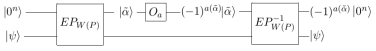
\includegraphics[scale=1.5]{./oracle}
\end{center}
L’algorithme de recherche d’un sommet marqué à l’aide d’une marche aléatoire
est alors analogue dans la forme à sa version classique.\\
Si l’on note :
\begin{itemize}
\item[- S :] coût de préparation de $ |U> $ (SETUP)
\item[- C :] coût de l’opération de vérification (Check)  $      |x> |y> \mapsto (-1)^{I_M(x)}|x>|y>$
 \item[- U :] coût de l’opération de mise à jour $W(P)$ (Update) : il s’agit du coût des
opérations $|x>|0>  \mapsto |x>|p_x> $ et $ |p_y>|y> \mapsto |0>|y> $ ainsi que leurs inverses.
\end{itemize}
La marche aléatoire quantique a la complexité suivante :


\begin{center}
\begin{boxedminipage}[ poslb ]{4cm}
\begin{center}
{\Large
$\mathit{S} + \frac{1}{\sqrt{\epsilon}}(C + \frac{1}{\sqrt{\delta}}U)$
}
\end{center}
\end{boxedminipage}
\end{center}
De même que dans le cas classique, on cherche à faire en sorte que $\mathit{C}$ soit dominé
par $ \frac{1}{\sqrt{\delta}}U $ , de sorte à avoir une complexité en $ O(\frac{1}{\sqrt{\delta \epsilon}}) $.

\subsubsection{Quantum Walk avec structure de données}

Étant donné un ensemble $\Omega$ on se donne une fonction $D : \Omega \rightarrow H_D$, qui
associe à un élément $x$ de $\Omega $ un élément  $D(x)$ de l’espace de Hilbert $H_D$. On
appellera structure de données l’ensemble $(D(x))_{x\in \Omega} $.
L’élément $ D(x) $ dépend souvent d’une fonction $f : \Omega  \rightarrow \left\lbrace  0, 1 \right\rbrace $ , dans ce cas on écrira $D_f (x)$ pour plus de clarté.\\
On s’intéresse donc au produit tensoriel $\ket{x} \ket{y}\ket{D(x)}$. Cela change les étapes
de l’algorithme de la manière suivante :
\begin{itemize}
\item[-] SETUP : Préparer $\ket{U_D} := \frac{1}{\sqrt{N}}\sum_{x,y=0}^{N-1} \ket{x} \ket{p_x}\ket{\mathit{D}(x)}$
\item[-]CHECK : $ \ket{x} \ket{y} \ket{ \mathit{D}(x)} \mapsto (-1)^{I_M(x)}\ket{x} \ket{y}\ket{\mathit{D}(x)} $
\item[-] UPDATE : cette étape fera intervenir en plus les fonctions $\ket{x}\ket{0}\ket{D(x)} \mapsto 
\ket{x} \ket{y}\ket{D(x)}$ et $\ket{x} \ket{y}\ket{D(x)} \mapsto \ket{x} \ket{y}\ket{D(y)}$ et leurs inverses.

\end{itemize}
Comme nous le verrons, l’intérêt de l’incorporation des structures de données
vient principalement du fait qu’elles permettent d’accélérer la vérification et
donc de diminuer $C$.\cite{Ghazal}

\subsection{Algorithme de Recherche de collisions}

Dans cet algorithme il s'agit de répondre au problème suivant:
\paragraph{Problème}: (Recherhe de collisions généralisée).Etant donné $f_i: S_i \rightarrow E,i=1,2,S_1,S_2    $ et $E$ des ensembles quelconques, trouver $(s_1,s_2)\in S_1 \times S_2 $ tel que $f_1(s_1)=f_2(s_2)$.\cite{Ghazal}\\
Dans l’algorithme qui résout ce problème à l’aide de l’algorithme de Grover
et que l’on nommera $CollisionGrover$, on commence par construire la liste\\
$L_1:=\left\lbrace (f_1(s_1),s_1)|s_1 \in S_1 \right\rbrace   $ et on la trie.\\
Ensuite, on définit la fonction $ C_{L_1}: S_2 \rightarrow \left\lbrace 0,1 \right\rbrace  $ comme suit:

\[ C_{L_1}(s_2)
\left \{
\begin{array}{c c}
   1 \hspace{0.3cm} \text{s'il existe}\hspace{0.3cm} s_1\hspace{0.3cm} \text{tel que} \hspace{0.3cm} (f_2(s_2),s_1)\in L_1\\
   0 \hspace{0.3cm} \text{sinon}
\end{array}
\right.
\]

Enfin, on se sert de l’algorithme de Grover pour trouver $s_2 \in S_2$ tel que
$C_{L_1}
(s_2) = 1 $ et on cherche le $s_1$ correspondant et on retourne $(s_1, s_2)$.
On donne le pseudo-code de cet algorithme :
\paragraph{Algorithme: $CollisionGrover $}\cite{Ghazal}-p19\\

\begin{itemize}
\item[\textbf{Entrées}]: $S_1,S_2,f_1,f_2 $
\item[\textbf{Sorties}]:$ (s_1,s_2)\in S_1 \times S_2  $ tels que $f_1(s_1)=f_2(s_2) $, NULL s'il n'y a pas de collision
\begin{enumerate}
\item $ L_1 \gets  $ Nouvelle liste
\item Construire et trier la liste $ L_1 $
\item Trouver $ s_2 \in S_2 $ tel que $C_{L_1}(s_2)=1  $ avec l'algorithme de Grover
\item \textbf{retourner} $ (s_1,s_2)  $ ou NULL si aucun tel élément n'a pu être trouvé
\end{enumerate}

\end{itemize}
Cet algorithme est une complexité totale $\tilde{O}\left(\left(\mid S_1\mid + \sqrt{\mid S_2\mid} \right)T_f  \right)   $ pour l'algorithme de Grover ait un intérêt dans ce cas, il faudrait avoir $\mid S_1 \mid <<\mid S_2 \mid  $, le cas optimal étant $\mid S_1 \mid =O(\sqrt{\mid S_2 \mid})   $.\\
Quant à la complexité en espace, on stocke $L_1$ qui est de taille $O(\mid S_1 \mid)$. Par
conséquent la complexité en espace est en $O(\mid S_1\mid )$



\section{Décodage par ensemble d’information (ISD)}

Étant donné un code C de paramètres $\left[ n, k\right] $ et sa matrice de parité $\mathit{H}$, on dit
que $S \subset \left\lbrace 1,\cdots, n\right\rbrace $ est un ensemble d’information si $\mid S \mid = k$. Une technique qui
est basée sur l’utilisation de tels ensembles pour le décodage du code s’appelle décodage par ensemble d’information ou information set decoding (ISD) en anglais.\\
Les détails des calculs de complexité et des affirmations autour des paramètres optimaux ainsi que le code pour calculer les courbes de complexité se trouvent dans l’appendice $\mathit{C}$.\cite{Ghazal}-p29
\subsection{ Algorithme de Prange}

Le premier algorithme ISD et le seul algorithme ISD à proprement parler est l’algorithme de Prange : un algorithme probabiliste de type Las Vegas qui échantillonne les ensembles d’information en espérant que le vecteur d’erreur solution e de poids t ait toutes ses positions d’erreurs dans le complémentaire de l’ensemble d’information $\overset{-}{S} $ $(\mid \overset{-}{S} \mid = n-k)$. Cela réduit ainsi le problème du décodage à celui de la résolution d’un système linéaire, une tâche de complexité polynomiale.
\subsubsection{Version classique}
On notera cet algorithme $\mathit{P}$.\cite{Ghazal}\\
L’algorithme est constitué d’une boucle sur les ensembles d’information possibles et pour chaque ensemble d’information, on procède comme suit :
\begin{enumerate}
\item On note A la sous-matrice de $\mathit{H}$ dont les colonnes sont indicées par $\overset{-}{\mathit{S}}$.
\item Si $\mathit{A}$ est inversible, on fait $\mathit{A}^{-1}
s = e$ et si $w_{H}(e) = t$, on retourne $e$.
\item Si une des conditions sur $\mathit{A}$ ou sur $e$ n’est pas vérifiée, on recommence avec un autre ensemble d’information.

\end{enumerate}
Ainsi le coût des opérations au sein de chaque tour de boucle est polynomial.\\
On dit qu’un ensemble d’information est bon si le tour de boucle retourne le bon vecteur $e$, ce qui arrive si la sous-matrice $\mathit{A}$ est inversible (cet événement
arrive dans $ 29\% $ des cas [3]) et que $w_H(e) = t$. Si l’on note      $\mathit{P}_{P}$ la probabilité de tomber sur un bon ensemble d’information, la complexité temporelle de cet algorithme est en $\tilde{O}(\frac{1}{\mathit{P}_{p}})$.

\begin{theorem} Si H est une matrice aléatoire, en notant $R := \frac{k}{n}$
et $\tau=\frac{t}{n}  $
, on a l’expression suivante pour l’exposant $\alpha_P$ de l’algorithme de Prange :
\begin{center}
\begin{boxedminipage}[ poslb ]{8cm}
{\Large
    $ \alpha_{p}(\mathit{R})=\mathit{H}(\tau)-(1-\mathit{R})\mathit{H}(\frac{\tau}{1-\mathit{R}})$}
\end{boxedminipage}
\end{center}
Et $\max_{R}(\alpha_{p})=0.1207019$ pour $ \mathit{R}=0.4537$

\end{theorem}


\begin{center}
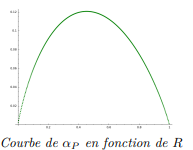
\includegraphics[scale=2]{./courbe_prange}
\end{center}
\paragraph{Démonstration :} Rappelons que le vecteur d’erreur devrait avoir la forme suivante :
les $t$ positions d’erreur sont parmi les $n-k$ indices de $\overline{\mathit{S}}$.\\
Par conséquent $\mathit{P}_{p}= \frac{{{n-k} \choose t }}{{n \choose t }}$, et l'algorithme a une complexité en $ \tilde{O}\left( \frac{{{n-k} \choose t }}{{n \choose t }}   \right) $. Afin d'avoir l'exposant de l'algorithme en fonction de $\mathit{R}$ (et d'autres paramètres). Nous utiliserons le théorème  $ {n \choose t} \approx 2^{n\mathit{H}(\frac{t}{n})}$ et on écrira $\mathit{R}:= \frac{k}{n}  $ et $ \tau = \frac{t}{n} $.
 

\begin{center}
{\Large
\[
\left.
\begin{array}{c @{\hspace{0.3cm}\vspace{0.2cm}\approx} c}
\frac{{n\choose t}}{{{n-k}\choose t}}& \frac{2^{nH(\frac{t}{n})}}{2^{(n-k)H(\frac{t}{n-k})}} \\
& \frac{2^{nH(\tau)}}{2^{n(1-R)H(\frac{\tau}{1-R})}} \\
& 2^{n(H(\tau)-(1-R)H(\frac{\tau}{1-R}))}
\end{array}
\right.
\]
}
\end{center}
On obtient ainsi l'expression suivante pour l'exposant $\alpha_{p}$:

\begin{center}
\begin{boxedminipage}[ poslb ]{8cm}
{\Large
    $ \alpha_{p}(\mathit{R})=\mathit{H}(\tau)-(1-\mathit{R})\mathit{H}(\frac{\tau}{(1-\mathit{R})}$
    }
\end{boxedminipage}
\end{center}
\subsubsection{Version quantique avec Grover}
On donne ici une version quantique de l’algorithme de Prange, donné pour la première fois dans [3], que l’on notera $\mathit{PG}$.
Dans cet algorithme, on part de la même hypothèse sur la répartition des erreurs (donc, si l’on note $\mathit{P}_{PG}$ la probabilité de tomber sur le bon ensemble d’information, on a $\mathit{P}_{PG} = \mathit{P}_{P}$ ). On utilise l’algorithme de Grover pour trouver le bon ensemble d’information (l’oracle pour l’algorithme de Grover s’obtient facilement en modifiant la suite d’étapes détaillée dans la partie précédente pour renvoyer 1 si l’ensemble d’information est bon et 0 sinon). Nous obtenons ainsi un algorithme de complexité temporelle $\tilde{O}\left( \sqrt{\frac{1}{\mathit{P}_{PG}}} \right)   $.\cite{Ghazal}
\begin{theorem} Si $\mathit{H}$ est une matrice aléatoire, en notant $\mathit{R} := \frac{k}{n}$ et $\tau := \frac{t}{n} $
, on a l’expression suivante pour l’exposant $\alpha_{PG}$ l’algorithme de Prange+Grover :
\begin{center}
\begin{boxedminipage}[ poslb ]{7cm}
{\Large
    $ \alpha_{PG}(\mathit{R})=\frac{\mathit{H}(\tau)-(1-\mathit{R})\mathit{H}(\frac{\tau}{1-\mathit{R}})}{2}$
    }
\end{boxedminipage}
\end{center}
Et $\max_{R}(\alpha_{PG})=0.0603509$ pour $ \mathit{R}= 0.4537$
\end{theorem}

\begin{center}
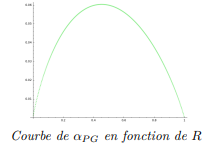
\includegraphics[scale=1.8]{./prange_grover}
\end{center}
\paragraph{Démonstration :} L’algorithme a une complexité temporelle en $ \tilde{O}\left( \sqrt{\frac{1}{\mathit{P}_{PG}}} \right) =\tilde{O}\left( \sqrt{ \frac{{n \choose t }}{{{n-k} \choose t }} }\right)  $.\\
On déduit l'expression suivante pour l'exposant $ \alpha_{PG}$:
\begin{center}
\begin{boxedminipage}[ poslb ]{7cm}
{\Large
    $ \alpha_{PG}(\mathit{R})=\frac{\mathit{H}(\tau)-(1-\mathit{R})\mathit{H}(\frac{\tau}{1-\mathit{R}})}{2}$
    }
\end{boxedminipage}
\end{center}


\section{Squelette d'un algorithme ISD}
Il y a d’autres algorithmes inspirés de l’algorithme de Prange et qui ont une meilleure complexité. On introduit un paramètre p en plus. Ces algorithmes
ISD "généralisés" échantillonnent des ensembles d’indices un peu plus généraux
que les ensembles d’informations, en espérant que la majeure partie, $t-p$, des
positions d’erreur soit dans le complémentaire de cet ensemble. Ils cherchent
ensuite les $p$ positions d’erreur restantes en se servant de stratégies efficaces
mais de complexité exponentielle.\\
Un algorithme ISD comporte donc une phase de recherche d’un ensemble d’indices
convenables suivi d’une phase de recherche d’un vecteur d’erreur vérifiant certaines
propriétés. Nous allons formaliser cette structure en donnant un squelette pour
ces algorithmes et en introduisant un cadre pour l’analyse de leur complexité.\\
La différence principale entre les algorithmes ISD réside dans la façon dont
ils trouvent le vecteur d’erreur. Chaque algorithme A fait appel à une fonction
$Recherche_A$ propre à elle, dont la spécification est la suivante :\\
$Recherche_A$: $ \mathit{S},\mathit{H},s,t,p \rightarrow \left\lbrace e \hspace{0.2cm} |\hspace{0.2cm} s=\mathit{H}e^T   \right\rbrace \cup \left\lbrace NULL \right\rbrace $\hspace{0.2cm} $e$ \hspace{0.1cm} est poids $p$ \hspace{0.1cm}sur $ \mathit{S}$ \hspace{0.2cm}  $t-p$ sur $\overset{-}{\mathit{S}}$
\hspace{0.2cm} où $\mathit{S}$ est un ensemble d'indices,$\mathit{H}$ la matrice de parité du code et $s$ le syndrome de l'erreur cherché.\\
Nous pouvons maintenant donner le squelette d'un algorithme ISD:
\begin{algorithm}
\caption{Squelette ISD } \cite{Ghazal}-p32
\begin{algorithmic}[1] 
\Require $\mathit{H}$,$y$,$s=\mathit{H}y^T$,$t$,$p$
\Ensure $e$ de poids $t$ tel que $s=\mathit{H}e^T $
\State \Repeat
\State Tirer un ensemble d’indices $\mathit{S} \subset \left\lbrace  1,\cdots, n \right\rbrace $
\State $e\gets Recherche_A(\mathit{S},\mathit{H},s,t,p)  $
    
    \State \Until{$w_H(e)=t $}
    \State \textbf{retourner} $e$
\end{algorithmic}
\end{algorithm}

\textbf{ Analyse de complexité} Comme nous l’avons dit, un tour de boucle de
l’algorithme débouche sur le bon vecteur d’erreur si ses positions d’erreurs sont
réparties d’une certaine manière (sa forme exacte dépend de l’algorithme A).
Si $\mathit{P}_A$ est la probabilité qu’il ait cette forme, il faut donc en moyenne  $\mathit{P}_A^{-1}$
répétitions de la boucle avant de le trouver. En réalité, il faut également que
la sous-matrice indicée par $\mathit{S}$ soit inversible, mais cela ne fait que multiplier le
nombre de tours de boucles par un facteur constant.
Le temps d’exécution de la fonction $Recherche_A$ dépend de l’algorithme A. On
le notera $\mathit{T}_A$. Cette fonction pourrait également avoir une complexité spatiale
non-négligeable que l’on notera $\mathit{S}_A$.\\
L’algorithme aura par conséquent une complexité temporelle en  $\~O(\mathit{P}_A^{-1}\mathit{T}_A ) $ et une complexité spaciale en $\mathit{S}_A $. \cite{Ghazal}\\
\textbf{Pour simplifier les notations} Dans ce qui suit, nous allons considérer une
version modifiée de l’algorithme présenté ci-dessus afin de faciliter la présentation
des algorithmes. En effet, étant donné un ensemble d’indices 
$\mathit{S}$ de taille $n-k$ tel que les colonnes indicées par
$
 r$
cet ensemble forment une sous-matrice inversible,
on considère $\mathit{P}\in\mathit{M}_{n,m}$ la matrice qui permute les colonnes de $ \mathit{H}$indicées par $  \mathit{S}$avec les dernières colonnes de $ \mathit{H}$. Alors, la matrice
 $  \mathit{HP}$
  possède une sous-matrice
carrée à droite. On peut alors faire un pivot de Gauss
 $\mathit{T}$ sur cette matrice afin
d’obtenir la matrice  $\mathit{THP}:=\tilde{\mathit{H}}=\left[\mathit{A}|\mathit{Id}_{n-k}\right]$,$  \mathit{A}\in \mathit{M}_{n-k,k}$.Alors,si l'on note $ \tilde{s}:=\mathit{T}s$ et $\tilde{e}:=e\mathit{P}$,on a:
\begin{enumerate}
\item Comme $\mathit{P}$ est une permutation, $w_H(\tilde{e})=w_H(\tilde{e}\mathit{P}^{-1})=w_H(e)=t$.
\item $\tilde{s}=\tilde{\mathit{H}}\tilde{e}^{T}\Leftrightarrow \mathit{T}s=\mathit{THP}(e\mathit{P})^{T}=\mathit{THP}\mathit{P}^{-1}e^{T}\Leftrightarrow \mathit{T}s=\mathit{TH}e^{T}\Leftrightarrow s=\mathit{H}e^{T}$
\end{enumerate}
Par conséquent, nous allons modifier l’algorithme de la manière suivante : on
transforme d’abord H et s en $\tilde{H}˜$ \hspace{0.1cm} et  $\tilde{s}$, puis on applique $Recherche_A$ à ces
arguments et à l’ensemble $\tilde{\mathit{S}}$ des $\mid S \mid $ derniers indices, ce qui fait qu’à la fin
de l’algorithme, le résultat est $\tilde{e}$ et on retourne ensuite $\tilde{e}\mathit{P}^{-1}=e$.\\
Cela étant un point de détail qui permet de faciliter la présentation, afin d’alléger la notation, dorénavant nous écrirons directement $\mathit{H}=\left[\mathit{A}|\mathit{Id}_{n-k}\right]$.
\subsection{Décodage par ensemble d'information quantique}

On rappelle la spécification et la complexité en requêtes de l’algorithme de
Grover.\\
$Grover : \epsilon , \left\lbrace f : E \rightarrow  \left\lbrace 0, 1\right\rbrace \right\rbrace  \rightarrow \ket{X}$ , où $\ket{X}$ est une superposition d’états $ x \in  E $
tel que $ f(x) = 1 $ . Cela s’effectue en $ O(\frac{1}{\sqrt{\epsilon}})   $
requêtes à la fonction $f$, où $\epsilon $ est la
proportion des $x \in E $  tel que $ f(x) = 1$.\\
Étant donné une matrice $\mathit{H}$, un syndrome $s$, des entiers $t$ et $p$ et un algorithme
de décodage générique $\mathit{A}$, on définit la fonction $\mathit{F}_A : S \rightarrow \left\lbrace 0, 1\right\rbrace $ comme la
fonction qui exécute  $RechercheA(S, \mathit{H}, s, t, p)$ et renvoie 1 si le vecteur renvoyé
n’est pas NULL et est de poids $t$ , et 0 sinon.\\
Alors, pour trouver une erreur de poids $t$ tel que $s = \mathit{H}e^T$
, il suffit d’utiliser
l’algorithme de Grover sur $\mathit{F}_A$ pour obtenir un ensemble d’indices $S$. Il suffit
ensuite d’appliquer $RechercheA$ avec cet ensemble d’indices.\\
Ainsi, un algorithme ISD quantique a la forme générale suivante :
\begin{flushleft}
\begin{boxedminipage}[ poslb ]{12cm}
\paragraph{Algorithme 5: Squelette ISD quantique }\cite{Ghazal},p32 \\

\begin{itemize}
\item[Entrées] : $ \mathit{H}, y,s=\mathit{H}y^T,t,p $
\item[Sorties] : $e $ de poids $t$ tel que $ s=\mathit{H}e^T $ 
\end{itemize}
\begin{enumerate}
\item $ \ket{S} \leftarrow Grover(P_A,\mathit{F}_A) $
\item $ \ket{S_0} \leftarrow Mesure(\ket{S})       $

\item $ e \leftarrow Recherche_A(S_0,\mathit{H},s,t,p) $
\item \textbf{retourner} $e$
\end{enumerate}
   
\end{boxedminipage}
\end{flushleft}

La fonction $\mathit{F}_A$ a la même complexité temporelle et spatiale que $Recherche_A$,
c’est-à-dire respectivement $\tilde{O}(T_A)$ et $\mathit{S}_A$. L’algorithme de Grover trouve $\mathit{S}$ au
bout de $ O(\sqrt{P_{A}^{-1}})$

requêtes à $\mathit{F}_A$, d’où une complexité temporelle totale de $ \tilde{O}(\sqrt{P_A^{-1}T_A})$. La complexité de l’étape 3 est $\tilde{O}(T_A)$ et donc la complexité
temporelle totale d’un algorithme ISD quantique est $ \tilde{O}(\sqrt{P_A^{-1}}T_A)$ 
(et sa complexité spatiale est $\tilde{O}(S_A)$).\\
Nous finissons par une remarque générale sur les algorithmes ISD : dans les
algorithmes classiques $\mathit{A}$ autres que Prange, $ P_{A}^{-1} \leq P_p^{-1} $ mais $ T_A >> P_p $. \\
En effet, $T_P$ est polynomial, mais dans tous les autres algorithmes $T_A$ est
exponentiel. Les algorithmes qui ont battu l’algorithme de Prange classique
ont réussi à avoir $ P_A^{-1} T_A < P_p^{-1}$
. Pour battre l’algorithme de Prange quantique,
on cherche des algorithmes A tels que q
$\sqrt{P_A^{-1}}T_A =
\sqrt{P_A^{-1} T_A^2 } < \sqrt{P^{-1}_{
PG}}$.
On va donc se focaliser sur l’algorithme RechercheA et les diverses façons de
l’améliorer en se servant d’algorithmes quantiques. De plus, en regardant la formule de complexité $ \sqrt{P_A^{-1}T_A}  $
, on se rend compte qu’il faut des améliorations
bien plus importantes qu’en classique pour battre $P_G$.

\section{Les algorithmes d'attaques ISD et ses dérivés}
 Depuis l'apparition du cryptosystème de McEliece en 1978, la sécurité a fait l'objet d'un certain nombre d'études d'un point de vue classique et quantique. Des efforts considérables ont été déployés dans le but de résoudre le problème du décodage par syndrome:\\
  \\Par exemple, Esser et Bellini \cite{Belestr5} ont proposé un estimateur, qui est un calcul plus réaliste des algorithmes ISD. \\ Narisada et al. introduisent, dans \cite{Narisada15}, des études sur le décodage des SDP à haute dimension en parallélisant des parties de l'algorithme ISD.\\
Cependant, il n'y a pas beaucoup d'études du point de vue quantique.\\
-En 2010, Bernstein \cite{Bergrover3} a proposé l'algorithme ISD quantique.\\
- Perriello et al \cite{Perriello18} ont proposé une attaque en utilisant l'algorithme de Bernstein pour BIKE et Classic McEliece.
 Ils ont ensuite amélioré cette attaque en utilisant la version quantique de l'algorithme de Lee-Brickell \cite{Leebr10}, qui est l'un des algorithmes de la DSI.\\
 - Esser et al \cite{Essramos6} ont également proposé une autre méthode d'attaque en utilisant l'algorithme de Bernstein, qui est l'un des algorithmes ISD et l'ont étendue à tous les candidats CBC lors du 4e tour du NIST PQC, y compris le HQC.\\
 - En 2017  Kachigar et Tillich \cite{Kati9} ont utilisés les algorithmes MMT \cite{Mmt11}, Grover,Quantum Walk,shamir-Schroeppel quantiques pour réduire davantage l'exposant de Prange .\\
 Malgré toute cette énergie consacrée, les meilleurs algorithmes ne donnent qu'une résolution exponentielle pour retrouver le vecteur d'erreurs $e$ de poids de Hamming $w$ pour un code binaire linéaire de longueur $n$ et de dimension $k$,avec un coût aproximatif  de $ \tilde{O}\left( 2^{\alpha\left( \frac{k}{n},\frac{w}{n} \right)n } \right) $ où $\alpha\left( \mathit{R},w\right)$ est positif quand $\mathit{R}$ et $w$ sont positifs.\\Nonobstant les recherches ne sont pas vaines car celles-ci ont permis de réduire legèrement l'exposant $\alpha\left( \mathit{R},w\right)$.\\Le tableau suivant donne un aperçu de la complexité temporelle moyenne des
algorithmes classiques existants lorsque $w$ est la distance de Gilbert-Varshamov $d_{GV}(n, k)$ du code telle que $d_{GV}(n, k)\overset{\Delta}{=} n \mathit{H}^{-1}_{2}\left( 1-\frac{k}{n} \right) $ où \\ $\mathit{H}_{2} \overset{\Delta}{=}-x\log_2(x)-(1-x)\log_2(1-x) $ est la fonction d'entropie binaire et son inverse $ \mathit{H}^{-1}_2 $ définie de $\left[ 0,1 \right] $ dans $ \left[0,\frac{1}{2} \right]$.Il correspond à la plus grande distance pour laquelle nous pouvons encore espérer une solution unique au problème du décodage. Si nous voulons que la solution soit unique, elle peut donc être considérée comme l'instance de décodage la plus difficile.\\
 Dans le tableau suivant, $w_{GV}$ est défini par le rapport $w_{GV}\overset{\Delta}{=}d_{GV}(n,k)/n$.
 \begin{table}
 \centering
\begin{tabular}{ |c|c|c|c| } 
\hline
Author(s)& Year& $\max_{0\leq R \leq 1}\alpha(R,w_{GV}) \hspace{0.2cm} to\hspace{0.2cm} 4 \hspace{0.2cm} dec.$ places \\
\hline
Prange [23] & 1962& $0.1207$\\
\hline
Dumer \cite{Dumer11} & 1991&$ 0.1164 $\\
\hline
MMT \cite{Mmt11} & 2011& $0.1114   $\\
\hline
BJMM \cite{Bjmm2} &2012&$ 0.1019   $\\
\hline
MO \cite{Mo19} &  2015& $0.0966 $\\
\hline

\end{tabular}
\caption{Les algorithmes ISD classiques}
\label{isd_classics}
\end{table}

La question de l'utilisation d'algorithmes quantiques pour accélérer les algorithmes de décodage de la ISD a été posée pour la première fois dans \cite{Over22}.
 Cependant, la façon dont l'algorithme de Grover a été utilisé dans ,\cite{Over22} sous-section 3.5] pour accélérer le décodage n'a pas permis d'obtenir des améliorations significatives par rapport aux algorithmes ISD classiques. Plus tard, Bernstein
 a montré dans \cite{Berst5} qu'il était possible d'obtenir des accélérations bien plus importantes avec l'algorithme de Grover: en l'utilisant pour trouver un ensemble d'informations sans erreur, l'exposant de l'algorithme de Prange peut en effet être réduit de moitié.\\
 Dans un article publié le 22 avril 2017 \cite{Kati9},Kachigar et Tillich  s'appuient sur  l'algorithme de recherche de Grover, ainsi que sur les algorithmes quantiques 
développés par Bernstein, Jeffery, Lange et Meurer dans \cite{Bernstein6} pour résoudre plus efficacement le problème de la somme des sous-ensembles. Le tableau suivant résume les ingrédients et la complexité temporelle moyenne
de l'algorithme de \cite{Berst5} et des nouveaux algorithmes quantiques présentés dans cet article.

\begin{table}
\centering
\begin{tabular}{ |c|c|c|c| } 
\hline
Author(s)& Year& Ingredients &$\max_{0\leq R \leq 1}\alpha(R,w_{GV}) \hspace{0.2cm} to\hspace{0.2cm} 4 \hspace{0.2cm} dec.$ places \\
\hline
Bernstein\cite{Berst5}& 2010&Prange $+$ Gr\footnotemark{}  & $0.06035$\\
\hline
 Kachigar- Tillich  & 2017& SS\footnotemark{}$+$Gr$+$QW\footnotemark{} &$ 0.05970 $\\
\hline
 Kachigar- Tillich & 2017&MMT$+$“1+1=0”$+$Gr$+$QW& $0.05869$\\
\hline

\end{tabular}
\caption{Les algorithmes ISD quantiques}
\label{isd_quantique}
\end{table}


En faisant une analogie  on voit que l'exposant de complexité de l'algorithme MMTQW apporte une amélioration d'une manière faible par rapport au meilleur algorithme ISD classique MO.
\subsection{Les Algorithmes de Prange et de Bernstein}
Rappelons que l'objectif est de trouver $e$ de poids $w$ étant donné $s^T=\mathit{H}e^T$ où $\mathit{H}$ est une matrice $(n-k)\times n$.
En d'autres termes, le problème que nous cherchons à résoudre consiste à trouver une solution à un système linéaire à n - k équations avec n variables et la solution est unique en raison de la condition de poids.\\
L'algorithme de Prange est basé sur l'observation suivante : si l'on sait que $k$ composantes données du vecteur d'erreur sont nulles, les positions d'erreur se trouvent parmi les $n-k$ composantes restantes. 
En d'autres termes, si l'on est sûr que les $k$ variables correspondantes ne sont pas impliquées dans le système linéaire, le vecteur d'erreur peut être trouvé en résolvant le système linéaire résultant de n-k équations à n-k variables en n-k variables en temps polynomial.\\
La difficulté consiste à trouver un ensemble de taille $k$ correct (d'indices des composants). L'algorithme de Prange échantillonne de tels ensembles et résout l'équation linéaire résultante jusqu'à ce qu'un vecteur d'erreur de poids $w$ soit trouvé.La probabilité de trouver un tel ensemble est de l'ordre de $\Omega\left( \frac{ {{n-k}\choose w}}{ { n\choose w}} \right)   $ et l'algorithme de Prange a donc une complexité 
\begin{center}

{\Large
$ \mathit{O}\left( \frac{{n \choose w}}{{{n-k}\choose w }} \right)= \tilde{\mathit{O}}\left( 2^{\alpha_{prange}(R,w)n} \right)    $
}
\end{center}
tel que 
\begin{center}
{\Large

$ \alpha_{prange}(R,w)=\mathit{H}_{2}(w)-(1-R)\mathit{H}_{2}\left(\frac{w}{1-R} \right)    $
}
\end{center}
en utilisant la formule binomiale connue
\begin{center}
{\Large
$ {n \choose w}= \tilde{\mathit{O}}\left( 2^{H_{2}(\frac{w}{n})n} \right)  $
}
\end{center}
L'algorithme de Bernstein consiste à utiliser l'algorithme de Grover pour trouver un ensemble de taille-k correct. En effet, un
oracle permettant de vérifier qu'un ensemble de taille-k est correct peut être obtenu en suivant les mêmes étapes que dans l'algorithme de Prange, c'est-à-dire en dérivant et en résolvant un système linéaire de $n-k$ équations à $n-k$ variables
et en retournant 1 si le vecteur d'erreur résultant a un poids w. Ainsi, la complexité de l'algorithme de Bernstein est la moitié de celle de l'algorithme de Prange,\\
\begin{center}

 i.e.\hspace{0.3cm} {\Large $\alpha_{Bernstein}=\frac{\alpha_{Prange}}{2}$}

\end{center}

Parmi les algorithmes ISD  ci-dessus  
certains ont une version classique et quantique(avec imbrication dans leur squelette ISD l'argorithme de grover quantique et la marche aléatoire sous forme de fonction d'où nous devons prendre compte implicitement leur complexité dans l'implémentation).\\
 De plus ils peuvent être classés suivant les ISD avancés avec technique des représentations et les ISD avancés avec techniques de représentations étendues cette nouvelle donne est obtenue avec la somme de sous-ensemble (subset-sum).
 
 \subsection{Les algorithmes ISD avancés avec technique de représentation}

Beaucoup d'algorithme n'ont pas permis  de réduire  la
complexité temporelle asymptotique de l’algorithme de Dumer à l'instar de l’algorithme de Shamir-Schroeppel . C’est l’utilisation
de la technique des représentations, une technique qui a été d’abord utilisée pour
accélérer la résolution du subset sum, qui va permettre d’accélérer la recherche
de collisions. L’algorithme de May, Meurer et Thomae ([12], [1]), que nous
allons décrire dans cette section et que nous noterons MMT, a été le premier
algorithme de décodage à utiliser cette technique.\cite{Ghazal}-p45
\paragraph{Considérations préliminaires }
\begin{enumerate}
\item On rappelle que l'on avait supposé, pour simplifier les notations, que $H=\left[ A | I_{n-k} \right]   $. Notons qu'on peut également écrire la matrice $ H  $ sous la forme 
$ H=\begin{bmatrix}
H'  |0_{h,n-k-h}\\
B   |I_{n-k-h}
\end{bmatrix}  $ avec $ H' \in \mathcal{M}_{h,k+h},B \in \mathcal{M}_{n-k-h,k+h}  $ . On considère plus précisément le code $\mathit{C'} $ obtenu en poinçonnés les $n-k-h  $ dernières colonnes de $G:=\left[ I_k | A^T \right]   $, qui est une matrice génératrice de $\mathit{C} $, la matrice génératrice $G' $ de $C' $ est alors donnée par la sous-matrice de $ G$ restreinte aux $k+h$ premières colonnes.Alors, d'après le théorème 11, la matrice $H' $ est une matrice de parité du code $ C' $. Qui plus est, puisque $G' $ admet une sous-matrice
inversible (la matrice identité), alors le théorème 10 entraîne que si l’on note $c:=mG  $, il est possible d'obtenir $c':=m_{|k+h} G' $, à partir de $c$ via l’opération de poinçonnage et inversement, il est possible de trouver c à
partir de c' de manière unique.\\
 On aura alors $ H'c^{'T}=0  $. On est donc ramené à un problème de décodage
par syndrome sur une matrice de taille plus petite, plus précisément une
matrice $(h+k)\times h $. Nous appelerons ce problème le problème de décodage par collision, d’après la technique principale qui sera utilisée pour le
résoudre. L’intérêt de se ramener à ce problème est que, bien qu’il y ait moins d’équations de parité (car $h$ est petit), le nombre de motifs d’erreurs possibles a diminué car on se restreint aux mots de codes de
poids $p$ du code C'.
\item De plus, pour optimiser la recherche de collisions, on fera l’hypothèse que les $p$ erreurs sont réparties de la manière  suivante dans la fenêtre de taille $k+h $:
\begin{figure}[htp]
\centering

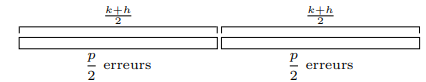
\includegraphics[scale=1.2]{./collision}


\end{figure}


\item Il est possible de décrire autrement le problème du décodage par collision,
à savoir avec des ensembles d’indices. En effet, si l’on note $M_l$ la $l_{ème}$ colonne d’une matrice $M$, alors les deux problèmes suivants sont équivalents :
\begin{itemize}
\item[(a)]: Trouver $e$ de longueur $n$ tel que $s=He^{T}  $ et $w_H(e)=t $.
\item[(b)] Trouver $ I \subset \left\lbrace 1,\cdots ,n\right\rbrace  , \mid I \mid =t$, tel que $s=\sum_{l \in I}H_l  $.

\end{itemize}
La deuxième formulation met en lumière des similitudes fortes avec le problème de la somme des sous-ensembles (subset sum) : le problème du décodage par collision peut être vu comme une version vectorielle du problème subset sum. Nous allons en effet commencer à nous servir de cette autre formulation.



\end{enumerate}


Dans la suite on fixe les notations suivantes :\\
$h=h_1 +h_2  $ et on va *diviser* $\mathit{H'} $ en deux sous-matrices ayant $h_1 $ et $h_2 $ lignes chacune.Pour simplifier les notations, nous allons définir $ \mathit{H}^{'(1)} $ comme étant la matrice $\mathit{H'} $ restreinte aux $h_1 $ premières lignes et $ \mathit{H^{'(2)}} $ comme étant la matrice $\mathit{H'} $ restreinte aux lignes $ h_1 +1 $ jusqu'à $h_1 + h_2=h $. Ainsi:
\begin{center}


$  
\mathit{H'}=\begin{bmatrix}
\mathit{H}^{'(1)}\\
\mathit{H}^{'(2)}
\end{bmatrix}
$
\end{center}
De même, pour un vecteur colonne $v$ de longueur $h$, on notera $v^{(1)}$ et $v^{(2)}$.\\
$y^{'} $ est le vecteur poinçonné de $y$





\subsubsection*{Algorithme MMT classique}

\paragraph{Technique des représentations }\cite{Ghazal} \\


\begin{enumerate}
\item Dans l’algorithme de Dumer comme dans l’algorithme de Shamir-Schroeppel,
nous avions considéré l’ensemble I des indices des composantes non-nulles du vecteur d’erreur e et nous l’avions écrit sous la forme $I =
I_1 \sqcup I_2 $ avec  $I_1 \subset \left\lbrace 1,\cdots,\frac{k+h}{2}
\right\rbrace $,  $I_2 \subset \left\lbrace  \frac{k+h}{
2} + 1,\cdots, k + h\right\rbrace $. On appelle
$(I_1, I_2)$ une représentation de l’ensemble I. L’idée de l’algorithme de
May, Meurer et Thomae est de relâcher les contraintes sur $(I_1, I_2)$ afin
d’avoir un nombre bien plus grand de représentations. En particulier,
nous n’exigerons plus que $\frac{p}{
2}$
erreurs soient réparties dans chaque moitié
du vecteur d’erreur. En faisant cela, on augmente de façon importante
la probabilité de tomber sur le bon vecteur d’erreur. Mais alors, un
nouveau problème surgit : en augmentant le nombre de représentations,
nous augmentons aussi la taille des listes. Nous verrons qu’il est possible
de choisir les paramètres de sorte à avoir une seule représentation qui
subsiste, ce qui diminue la taille des listes, mais garde l’avantage procuré
par la multiplicité des représentations. Cela nous permettra de réduire
aussi bien la complexité en l’espace qu’en temps.

\item L’algorithme de May, Meurer et Thomae repose donc sur la méthode des
représentations pour améliorer les complexités en temps et en espace.
Mais il y a aussi un deuxième niveau d’amélioration dans la mesure où
nous nous servons d’une recherche de collisions pour trouver les bonnes
représentations. Cela réintroduit des contraintes sur la forme du vecteur
d’erreur, mais comme nous le verrons plus tard, ces contraintes font
perdre au plus un facteur polynomial.

\end{enumerate}

\paragraph{Description de l'algorithme  }\cite{Ghazal}\\


On rappelle que l'ensemble $ \mathit{S}= \left\lbrace I \subset \left\lbrace  1,\cdots,h+k \right\rbrace  | \mid I \mid =p  \right\rbrace  $ est isomorphe à
l’ensemble des vecteurs d’erreur de poids $p$ et de longueur $k + h$. On cherche à
représenter l’ensemble $  \mathit{I}^{'} $ des coordonnées non-nulles du vecteur d’erreur comme $ I_1 \sqcup I_2 $ avec $ I_i \subset \left\lbrace 1,\cdots, k+h\right\rbrace , \mid I_i \mid =\frac{p}{2} $ pour $ i=1,2 $. Il y a $ p\choose {p/2}   $ telles représentations.\\
On prend :

\[
\left \{
\begin{array}{ c @{=} c c}
   J_{1,1} & J_{2,1} & \left\lbrace 1,\cdots,\frac{k+h}{2} \right\rbrace \\
   J_{1,2} & J_{2,2} & \left\lbrace  \frac{k+k}{2}+1,\cdots,k+h \right\rbrace 
   
\end{array}
\right.
\]

Alors $ S_{i,j}=\left\lbrace I_{i,j} \subset J_{i,j} | \mid I_{i,j}\mid =\frac{p}{4}  \right\rbrace     $ et $ \mid S_{i,j} \mid={{\frac{k+h}{2}}\choose {\frac{p}{4}}} \approx {{k+h}\choose {\frac{p}{2}}}^{1/2} $.

On construit les listes $ L_{i,j} $ à partir des $ S_{i,j} $, puis on construit les listes $ L_i $ à partir des listes $L_{i,j}  $,en considérant l'union exclusive $  \sqcup $ des ensembles d'indices.Par contre pour construire $L$ à partir des $L_{i}$, nous prendrons des ensembles d'indices $ I'=I_1 \bigtriangleup I_2     := (I_1\cup I_2)\setminus (I_1 \cap I_2)$, puisqu'il n'y a aucune garantie que les $ I_i \in L_i  $ soient disjoints.\\ 
Cette façon de construire les choses entraîne que $\mathit{I'}$ ne s'écrit tout à fait comme $ I_1 \cap I_2  $ avec $ I_i \subset \left\lbrace 1,\cdots,k+h \right\rbrace , \mid I_i \mid =\frac{P}{2}$, car avec cette construction, les $I_i  $ s'écrivent comme $I_{i,1}\sqcup I_{i,2}  $\\
L'intérêt de la méthode des réprésentations: en augmentant le nombre de façons de représenter un ensemble d'indices comme union de sous-ensembles, on arrive à réduire la taille des vecteurs cherchés par un facteur $ 2^{h_1}  $, ce qui réduit la taille
des listes de recherche et améliore donc la complexité, tout garantissant qu’il suffit de répéter un nombre constant de fois le procédé avant de tomber sur la bonne réponse.

La construction des listes se fait suivant l'algorithme $DecodeCollision_{MMT}$ ci-dessous en utilisant le sous programme merge-join


\begin{flushleft}
\begin{boxedminipage}[ poslb ]{15cm}

\paragraph{Algorithme 6 : $DecodeCollision_{MMT}$ }\cite{Ghazal} \\

\begin{itemize}
\item[\textbf{Entrées}]:$ \mathit{H}^{'},y^{'},s^{'}=H^{'}y^{'T},p,h_1,h_2,r $ vecteur de longueur $h$ tel que 
\item[] $ r^{(2)}=0,(S_{i,j})_{i,j=1,2}  $ 
\item[\textbf{Sorties}]: une liste $L$ d'ensembles $ \mathit{I}^{'} $, $ \mid  \mathit{I}^{'} \mid =p $ tels que $ \sum_{ l \in I^{'}} \mathit{H}^{'}_{l}=s^{'}  $
\end{itemize}
\begin{enumerate}
\item $ r_1 \gets r  $
\item $ r_2 \gets s'-r  $
\item Initialiser les listes $  L_{1,1},L_{1,2},L_{2,1},L_{2,2}  $
\item \textbf{pour} $i=1,2$ \textbf{faire}
\item \hspace{0.4cm} \textbf{pour} $ I_{i,1} \in S_{i,1}  $ \textbf{faire}
\item \hspace{0.8cm} $ L_{i,1} \gets L_{i,2} \cup (\sum_{l \in I_{i,1}} \mathit{H}_{l}^{'(1)},I_{i,1}) $
\item \hspace{0.4cm} \textbf{pour} $ I_{i,2} \in S_{i,2} $ \textbf{faire}
\item \hspace{0.8cm} $ L_{i,2} \gets L_{i,2} \cup (r_{i}^{(1)}+ \sum_{l \in I_{i,2}} \mathit{H}_{l}^{'(1)},I_{i,2}) $
\item \hspace{0.4cm} $ L_{i}(r) \gets L_{i,1} \Join_{h_1}^{r_i} L_{i,2} $ (*)
\item $ L \gets L_{1}(r)\Join_{h_2}^{s'}L_{2}(r)  $ (**)

\item \textbf{retourner L}

\end{enumerate}

   
\end{boxedminipage}
\end{flushleft}
(*)$ (L_{i,1}\Join_{h_1}^{r_i} L_{i,2}:= ((\sum_{l \in I_{i}}H_{l}^{'(2)},I_i)| I_i:=I_{i,1}\sqcup I_{i,2} \hspace{0.3cm}  tel \hspace{0.2cm} que \hspace{0.2cm} \sum_{l \in I_{i,1}} H_{l}^{'(1)}= r_{i}^{(1)} + \sum_{l \in I_{i,2}} H_{l}^{'(l)}))    $\\
(**)  $ L_{1}(r)\Join_{h_2}^{s'}L_{2}(r)=(I' | I':=I_{1}\bigtriangleup I_{2} \hspace{0.2cm} \mid I' \mid=p \hspace{0.2cm} tel \hspace{0.2cm} que \hspace{0.2cm}  \sum_{l \in I_{1}} H_{l}^{'(2)}=s^{'(2)} + \sum_{l \in I_{2}} H_{l}^{'(2)}  )    $\\
\textbf{Preuve de correction} de  $ DecodeCollision_{MMT}  $
\begin{itemize}
\item[•] La liste $L_1 $ contient les $I_{1}=I_{1,1} \sqcup I_{1,2}  $ tels que $ r^{((1))}=r_{1}^{(1)}=\sum_{l \in I_{1,1}}H_{l}^{'(1)} + \sum_{l \in I_{1,2}}H_{l}^{'(1)}=\sum_{l \in I_{1}}H_{l}^{'(1)}  $. 

\item[•] La liste contient les 
 $I_{2}=I_{1,2} \sqcup I_{2,2}    $ tels que $ s^{'(1)}-r^{(1)}=r_{2}^{(1)}= \sum_{l \in I_{2,1}} H_{l}^{'(1)} + \sum_{l \in I_{2,2}}H_{l}^{'(1)}= \sum_{ l \in I_2} H_{l}^{'(1)} .$ 
 
 \item[•] On a  $ \mid I_i \mid = \frac{p}{2} $ pour $ i=1,2 $ par construction car $ I_{i,1}  \cap I_{i,2}=\emptyset $. De plus, $I'=I_1 \bigtriangleup I_2 $ vérifie $ \mid I' \mid \leq p $
 
 
 \item[•] La liste \textbf{L} contient les $ I'= I_1 \bigtriangleup I_2  $  tels que:
 \[
\left \{
\begin{array}{c @{=} c}
   I_1 \in L_1 , \hspace{0.2cm} i.e. \hspace{0.2cm} \sum_{ l \in I_1} H_{l}^{'(1)}& r^{(1)}\\
    I_2 \in L_2 ,\hspace{0.2cm} i.e. \hspace{0.2cm} \sum_{ l \in I_2} H_{l}^{'(1)} &s^{'(1)}-r^{(1)}\\
    \sum_{ l \in I_1} H_{l}^{'(2)} + \sum_{l \in I_2} H_{l}^{'(2)}& s^{'(2)}\\
    \mid I' \mid=p ,\hspace{0.2cm} i.e. \hspace{0.2cm} I_1\cap I_2&\emptyset
   
\end{array}
\right.
\]

\[\Rightarrow
\left \{
\begin{array}{c @{=} c}
  \sum_{ l \in I_1} H_{l}^{'(1)} + \sum_{l \in I_2} H_{l}^{'(1)}& s^{'(1)}\\
  \sum_{ l \in I_1} H_{l}^{'(2)} + \sum_{l \in I_2} H_{l}^{'(2)}& s^{'(2)}\\
  \mid I' \mid & p 
\end{array}
\right.\\
\]

$\Rightarrow \sum_{l \in I'} H_{l}^{'}=s'$ et $ \mid I'\mid=p $

\end{itemize}
Par conséquent la liste de sortie \textbf{L} est bien comme on souhaite.
\paragraph{Analyse de complexité } \cite{Ghazal}\\

\begin{enumerate}
\item On parcours $ \mid S_{i,j} \mid $ éléments pour construire la liste $L_{i,j}  $ pour $ i,j=1,2 $.
\begin{itemize}
\item[•] Complexité en temps : $ \tilde{O}(\mid S_{i,j} \mid)  $
\item[•] Complexité en espace : $ \mid L_{i,j} \mid = \mid S_{i,j} \mid \Rightarrow \tilde{O}(\mid S_{i,j} \mid)$
\end{itemize}
\item Pour construire $L_1$ et $L_2$, on fait un Merge-Join sur des listes de taille
$\mid L_{i,j} \mid$ contenant des vecteurs binaires de longueur $h_1$.
\begin{itemize}
\item[•] Complexité en temps : $\tilde{O}\left( \max\left( \mid L_{i,j} \mid ,{ \mid L_{i,j}  \mid}^{2}2^{-{h_1}}\right)  \right)   $
\item[•] Complexité en espace: $ \mid L_i \mid =\tilde{O}\left( {\mid L_{i,j} \mid}^{2}2^{-{h_1}}  \right)\Rightarrow \tilde{O}\left(  \max\left( \mid L_{i,j} \mid,\mid L_i \mid \right)  \right)   $ 
\end{itemize}

\item Pour construire $L$, on fait un Merge-Join sur des listes de taille $ \mid L_i \mid $
contenant des vecteurs binaires de longueur $h_2$.

\begin{itemize}
\item[•] Complexité en temps: 
$\tilde{O}\left( \max\left( \mid L_{i} \mid ,{ \mid L_{i}  \mid}^{2}2^{-{h_2}}\right)  \right) = \tilde{O}\left( \max\left( {\mid L_{i,j} \mid}^{4}2^{-2{h_1}-{h_2}} ,{ \mid L_{i,j}  \mid}^{2}2^{-{h_1}}\right)  \right)    $
\item[•] - Complexité en espace : on peut réutiliser de l’espace mémoire $ \Rightarrow O(1)$.

\end{itemize}

\end{enumerate}


\subsubsection{Complexité}
\begin{theorem} \cite{Ghazal} Si H est une matrice aléatoire, en notant $ R:=\frac{k}{n} $,$  \tau:=\frac{t}{n} $, $\pi:=\frac{p}{n} $ et $ \eta :=\frac{h}{n} $, on a l'expression suivante pour l'exposant $\alpha_{MMT} $ de l'algorithme de MMT:
\begin{center}
$ \alpha_{MMT}(R)=\min_{\pi,\eta}(\beta(R,\pi,\eta)+ \max_{i=1,2,3}\gamma_i(R,\eta,\pi) )  $ avec
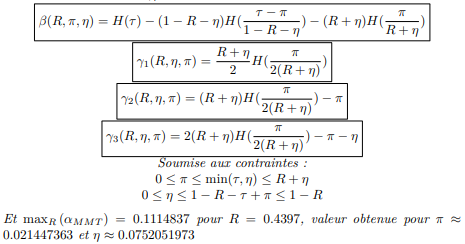
\includegraphics[scale=1.2]{./theo}
\end{center}

\end{theorem}


\textbf{Complexité en temps de } $DecodeCollision_{MMT}  $\\
\begin{center}


$ \tilde{O}(\max (\mid S_{i,j} \mid,{\mid S_{i,j} \mid}^{2}2^{-h_1},{\mid S_{i,j} \mid}^{4}2^{-2h_1-h_2}) )    = \tilde{O}\left( \max\left(  {{k+h}\choose {\frac{p}{2}}}^{\frac{p}{2}},{{k+h}\choose {\frac{p}{2}}}2^{-h_1} , {{k+h}\choose {\frac{p}{2}}}^{2}2^{-2h_1-h_2}\right)  \right)      $\\
\end{center}
\textbf{Complexité en espace de} $DecodeCollision_{MMT}   $\\
\begin{center}


$ \tilde{O}(\max (\mid S_{i,j} \mid,{\mid S_{i,j} \mid}^{2}2^{-h_1}) )   = \tilde{O}\left( \max \left( 
{{k+h}\choose {\frac{p}{2}}}^{\frac{1}{2}},{{k+h}\choose {\frac{p}{2}}}2^{-{h_1}}
\right)  \right)   $
\end{center}

\paragraph{Algorithme de recherche MMT}

Cet algorithme est décrit comme ci-dessous en se basant sur la recherche d'un bon vecteur

\begin{flushleft}
\begin{boxedminipage}[ poslb ]{15cm}

\paragraph{Algorithme 7:$Recherche_{MMT}$ }\cite{Ghazal}\\
\begin{itemize}
\item[\textbf{Entrées}]: $\mathit{H},y,s=\mathit{H}y^T,t,p,h_1,h_2,(S_{i,j})_{i,j=1,2}  $
\item[\textbf{Sortie}] : $e$ tel que $ y=mG+e  $ et $  w_{H}(e)=t $,NULL si aucun tel vecteur \\ n'a pu être trouvé
\end{itemize}
\begin{enumerate}
\item Préparer $ G',H',y' $ et calculer $ s'=H'y^{'T} $
\item \textbf{pour} tous les vecteurs $r$ de longueur $h$ tel que $ r^{(2)}=0  $ \textbf{faire}
\item \hspace{0.3cm} $ L \gets DecodeCollision_{MMT}(H',y',s',p,h_1,h_2,r,(S_{i,j})_{i,j=1,2})  $
\item \hspace{0.5cm} \textbf{pour} $ I' \in L $ \textbf{faire}
\item \hspace{0.8cm} $ e \gets Depoinçonner(I')
 $
 \item \hspace{0.8cm} \textbf{si} \hspace{0.2cm} $w_{H}(e)=t  $ \hspace{0.2cm} \textbf{alors}
 \item \hspace{0.8cm} \textbf{retourner e}
 \item \textbf{retourner} NULL
 
\end{enumerate}
\end{boxedminipage}
\end{flushleft}


$Recherche_{MMT}$ fait appel à l'algorithme $DecodeCollision_{MMT} $ pour obtenir la liste $L$ à part
ir de laquelle l'ensemble d'indices $I' $ est dépoinçonné pour un vecteur $e$ s'il est de poids $t$ sinon l'algorithme retourner $ NULL $
 ceci est bouclé sur $2^{h_1} $ éléments au maximum avec $h_1=\log_2{p \choose {\frac{p}{2}}} $ \\ \textbf{la complexité en temps de} $ Recherche_{MMT}$ est la même que celle de $DecodeCollision_{MMT} $ à savoir :
 \begin{center}
 $T_{MMT}= \tilde{O}\left( \max\left(  {{k+h}\choose {\frac{p}{2}}}^{\frac{1}{2}},{{k+h}\choose {\frac{p}{2}}}2^{-p} , {{k+h}\choose {\frac{p}{2}}}^{2}2^{-2p-(h-p)}\right)  \right)   $
 \end{center}
 On en déduit la complexité de l'algorithme:\\
 \begin{center}
 $ \tilde{O}\left(\frac{{n\choose t}}{{{k+h}\choose p}{{n-k-h}\choose{t-p}}} \max\left(  {{k+h}\choose {\frac{p}{2}}}^{\frac{1}{2}},{{k+h}\choose {\frac{p}{2}}}2^{-p} , {{k+h}\choose {\frac{p}{2}}}^{2}2^{-2p-(h-p)}\right)  \right)  $
 
 \end{center}
 \begin{tipblock}
L’intérêt de la méthode des représentations : en augmentant le nombre de façons de
représenter un ensemble d’indices comme union de sous-ensembles, on arrive à
réduire la taille des vecteurs cherchés par un facteur $2^{h_1}$
, ce qui réduit la taille
des listes de recherche et améliore donc la complexité, tout garantissant qu’il
suffit de répéter un nombre constant de fois le procédé avant de tomber sur la
bonne réponse.

\end{tipblock}

\begin{figure}[htp]
\centering
\begin{center}

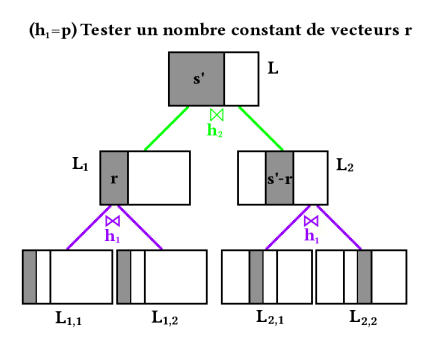
\includegraphics[scale=1.2]{./arbre}
\caption{$Recherche_{MMT}$- illustration sous forme d'arbre \\
Violet: recherche de collisions classiques\\
vert: technique des représentations\\
$\Join $:Merge-Join} \cite{Ghazal}
\label{fig:mmt1}
\end{center}

\end{figure}

\subsubsection{Algorithme de May, Meurer et Thomae quantique avec Quantum Walk}
 
Dans cette partie il s’agit de résoudre le problème
du décodage par collision à l’aide d’une marche aléatoire quantique. En effet,
nous pouvons reformuler le problème que cherchent à résoudre les fonctions
RechercheSS et RechercheMMT comme le problème de recherche de 4-uplet
suivant :\\
\textbf{Problème 7} \cite{Ghazal} (Décodage comme recherche de 4-uplet). Soit 



\[
\left.
\begin{array}{c  c}
f: S_{1,1} \times S_{1,2}  \times S_{2,1}\times S_{2,2}\longrightarrow \mathbb{F}_{2}^{h} \\
f:(I_{1,1},I_{1,2},I_{2,1},I_{2,2})\mapsto \sum_{i,j=1,2}\sum_{l \in I_{i,j}} {H'}_{l}+s  
   
\end{array}
\right.
\]
Trouver  $4-uplet(I_{1,1},I_{1,2},I_{2,1},I_{2,2})$  tel que $ f(I_{1,1},I_{1,2},I_{2,1},I_{2,2})=0$   et
$ \mid \cup_{i,j=1,2}I_{i,j} \mid=p $.\\

Or, nous avons vu qu’il peut être intéressant d’utiliser une marche aléatoire
pour résoudre des problèmes qui admettent ce type de formulations. C’est
effectivement le cas : comme nous le verrons, si certaines conditions sont réunies,
la marche aléatoire quantique permet de contourner le problème du goulot
d’étranglement qui se posait avec l’algorithme de Grover. De plus, la recherche
du bon vecteur d’erreur parmi les éléments de la liste finale peut se faire au sein
de la marche aléatoire, ce qui évite le recours à des recherches imbriquées qui
augmentent la complexité comme dans DG
\subsubsection{Squelette d’un algorithme ISD avancé avec Quantum Walk}
\paragraph{La marche aléatoire et son graphe} \cite{Ghazal} La solution cherchée est un $4-uplet (I_{1,1},I_{1,2},I_{2,1},I_{2,2}) \in S_{1,1} \times S_{1,2} \times S_{2,1} \times S_{2,2}$. 
Pour éviter de parcourir tout
l’espace de recherche, on va considérer quatre sous-ensembles $ T_{i,j} $ des ensembles
$ S_{i,j} $ , tous de même taille $T \leq \mid S_{i,j} \mid $. \\
A l'aide de ces identifications, on considère donc une marche aléatoire sur le graphe $J(4\mid S_{i,j} \mid,4T)  $ pour trouver un $4-uplet$ convenable pour une fonction $ f_A$
que l'on définira ci-dessous. Il s'agit de la marche $  QW(J(4\mid S_{i,j} \mid,4T),f_A)  $ en reprenant une notation introduite dans la section sur l'algorithme quantique.\\
On a besoin de définir ou expliciter les éléments suivants :
\begin{enumerate}
\item Le trou spectral $ \delta=\frac{4\mid S_{i,j} \mid}{4T(4(\mid S_{i,j} \mid-4T))}=\Omega(T^{-1}) $
\item La fonction $f_A$ à calculer et la structure de données associée.
\item L’ensemble des éléments marqués $M_{fA}$ , ce qui donnera la proportion $\epsilon$
des éléments marqués.
\item Le coût $\mathit{S}$ de Setup.
\item Le coût $\mathit{C}$ de Check.
\item Le coût $\mathit{U}$ de Update.
\end{enumerate}
\paragraph{La fonction $f_A$ et la structure de données associée}
 La fonction $f_A$ a à
peu de choses près la même structure que les fonctions $DecodeCollision_A$ des
algorithmes ISD avancés.


En effet, elle calcule des structures de données ordonnées contenant des couples
"($\sum_{J},J  $)", où $J$  désigné un ensemble d’indices, sur trois niveaux, où celles du
niveau le plus bas sont générées directement et celles du niveau suivant sont
obtenues à partir de celles du niveau précédent en faisant un Merge-Join et
en exigeant une égalité à un vecteur d’abord sur $h_1$ coordonnées et ensuite sur
les $h_2$ coordonnées restantes.\\
Ainsi, la fonction $f_A$ créé quatre structures de données $D_{f_{i,j}}, i = 1, 2$ au dernier
niveau, puis deux au niveau suivant, $D_{f_1}$
et $D_{f_2}$
. Ces structures de données sont
ordonnées en fonction du premier élément du couple. Enfin, au niveau final, une
dernière structure de données $D$ est créée à partir de $D_{f_1}$
et $D_{f_2}$
. Dans cette
structure de données, toutes les sommes sont égales et donc on peut se contenter
de ne stocker que l’ensemble d’indices $J$.\\

Ce qui change des fonctions $DecodeCollision_A$, c’est que tout d’abord, $f_A$
stocke en parallèle les ensembles d’indices séparément à chaque niveau dans des
structures de données ordonnées. Elle créé ainsi quatre structures de données
$D_{I_{i,j}} , i, j = 1, 2$ au niveau le plus bas, puis deux, $D_{I_1}$
et $D_{I_2}$
au niveau suivant.\\
Par conséquent, la structure de données associée à la fonction $f_A$ comporte ainsi
treize sous-structures de données $(D_{I_{i,j}} )_{i,j=1,2},(D_{f_{i,j}} )_{i,j=1,2},(D_{I_i}
)_{i=1,2},(D_{fi
})_{i=1,2}, D$.\\
Enfin, $f_A$ diffère des fonctions $DecodeCollision_A$ dans la mesure où, après avoir
crée la structure de données finale D, elle cherche s’il existe $I' \in D $ tel que, en
y appliquant l’opération $Dépoinçonner$, on tombe sur un vecteur d’erreur $e$ de
poids $t$. Elle renvoie $0$ si c’est le cas, 1 sinon.\\

La fonction $f_A$  est définie comme suit:
\begin{flushleft}
\begin{boxedminipage}[poslb]{15cm}
\paragraph{Algorithme 8: $f_A$ }\cite{Ghazal}\\
\begin{itemize}
\item[\textbf{\textbf{Entrées}}]: $T_{i,j}$ pour $ i,j=1,2,r $ vecteur de longueur $h$ tel que $r^{(2)}=0 $
\item[] $ H',y',s'=H'y^{'T},p,h_1,h_2  $
\item[\textbf{Sorties}]:une liste $L$ d'ensembles $ I' $, $\mid I' \mid=p $ tels que $ \sum_{l \in I'}{H'}_{l}=s'$
\end{itemize}
\begin{enumerate}
\item $r_1 \gets r  $  
\item $ r_2 \gets s'-r  $
\item Initialiser et remplir les $ D_{I_{i,j}}  $ et $ D_{f_{i,j}} i,j=1,2 $
\item \textbf{pour} $i=1,2$ \textbf{faire}
\item \hspace{0.8cm} $ D_{f_i}(r) \gets D_{f_{i,1}} \Join_{r_i}^{h_1}D_{f_{i,2}} $
\item \hspace{0.8cm} $ D_{I_i}(r) \gets D_{I_{i,1}} \Join_{r_i}^{h_1}D_{I_{i,2}} $
\item $D \gets D_{f_{1}} \Join_{h_2,\mid I' \mid=p}^{s'}D_{f_{2}} (r)  $

\item \textbf{si} on peut trouver $e$ de poids $t$ à partir de $D $ \textbf{alors}

\item \hspace{0.8cm} \textbf{retourner} 0
\item \textbf{sinon}
\item \hspace{0.8cm} \textbf{retourner} 1

\end{enumerate}

\end{boxedminipage}

\end{flushleft}
\textbf{La proportion $\epsilon $ des éléments marqués} \\ On définit \hspace{0.3cm} $M_{f_A}:="\left\lbrace I' | w_{H}(e)=t \hspace{0.3cm} \text{où} \hspace{0.3cm} e=Dépoinconner(I) \right\rbrace   "   $.

Sous l'hypothèse d'avoir choisi le bon vecteur $r$, la structure de données $D$ contient des ensembles $ I' $ qui s'écrivent $ I_1 \diamond I_2 =(I_{1,1}\sqcup I_{1,2})\diamond (I_{2,1} \sqcup I_{2,2})$ avec $\diamond \in \left\lbrace \sqcup,\bigtriangleup \right\rbrace   $ en fonction de l'algorithme. La probabilité qu'un seul des $T_{i,j}   $ contienne l'ensemble $ I_{i,j} $ en question est $\frac{T}{\mid S_{i,j} \mid}  $. Comme les $T_{i,j}$ sont indépendants,la probabilité de succès $ \epsilon $ est donc $ \left(\frac{T}{\mid S_{i,j} \mid} \right)^{4}  $


Le squelette de la fonction de $Recherche_A $:
\begin{flushleft}
\begin{boxedminipage}[poslb]{15cm}
\paragraph{Algorithme 9: $MMTQW$ }\cite{Ghazal}\\
\begin{itemize}
\item[\textbf{\textbf{Entrées}}]: $ H,y,s=Hy^{T},p,t $

\item[\textbf{Sorties}]:\hspace{0.2cm}$e$ tel que $s=mG+e $ et $w_H(e)=t$, $NULL  $ si aucun tel vecteur \\ n'a pu être trouvé
\end{itemize}
\begin{enumerate}
\item Préparer $G',H',y' $ et calculer $s'=H'y^{'T}  $
\item $|p>\gets Grover(R_A^{-1},QW_A) $
\item $r \gets Mesure(|p>)  $
\item $I'=(I_{1,1},I_{1,2},I_{2,1},I_{2,2})    \gets QW(J(4\mid S_{i,j} \mid,4T),f_A(\cdots,r,\cdots)) $
\item $ e \gets Dépoinçonner(I') $
\item \textbf{retourner} $e$


\end{enumerate}

\end{boxedminipage}

\end{flushleft}
On rappelle $ Grover(\epsilon,f) $ pour la recherche d'un $x$ tel que $f(x)=1  $ avec l'algorithme de Grover, et on rappelle que l'on a défini la marche $QW(J(4\mid S_{i,j} \mid,4T),f_A)     $ ci-dessus.\\
Puis, on définit la fonction $QW:r\mapsto\left\lbrace 0,1 \right\rbrace    $
comme la fonction qui renvoie 1 ssi $QW(J(4\mid S_{i,j}\mid,4T),f_A)  $ trouve un bon $4-uplet  $ lorsque $f_A  $ prend en argument r.\\
\paragraph{Complexité} Sous l'hypothèse d'avoir le bon vecteur $r$,la marche aléatoire trouve le bon vecteur d'erreur $e$ en temps \cite{Ghazal}
\begin{center}

\[
\left.
\begin{array}{c @{=} c}
S + \frac{1}{\sqrt{\epsilon}}(C+\frac{1}{\sqrt{\delta}}U) & O(T)+ {\mid S_{i,j} \mid}^{2}T^{-2}(\tilde{O}(1)+O(\sqrt{T})O(1))  \\
& \max(T,{\mid S_{i,j} \mid}^2T^{-3/2})
   
   
   
\end{array}
\right.
\]

\end{center}
Il faut ajouter à ce coût le coût de la recherche du bon vecteur $r$ parmi $R_A  $ possibilités, ce qui est faisable en temps $O(\sqrt{R_A}) $ avec l'algorithme de Grover. Ainsi le coût total sera $\tilde{O}(\sqrt{R_A}\max(T,{\mid S_{i,j} \mid}^2T^{-3/2}))  $

\subsubsection{Algorithme MMTQW}

\paragraph{Impossibilité d'une approche directe}\cite{Ghazal}  une adaptation directe de MMT ne marche pas car le choix de $ h_1$ et $ h_2$ est imposé et pour avoir  exactement une représentation de chaque ensemble de positions
d’erreur, il faut prendre $ h_1 = p$. D’autre part, pour garder l’équilibre qui
fait fonctionner l’algorithme, il faut prendre $h1 = \log_2(T)$. Par conséquent, on
devrait avoir $p = \log_2(T)$, or on devrait avoir $p < t$, mais dans les cas qui nous
intéressent on a $\log_2
(T) > t$, par conséquent la totalité des conditions souhaitées
sur les paramètres ne peuvent pas être vérifiées.\\ Pour pallier à ce problème, nous allons opter pour \textbf{un algorithme hybride entre MMT et SS(Shamir-Schroeppel)} Cet algorithme, que l’on note
$MMTQW$, utilise la technique des représentations. Il s’agit en effet de prendre
le cas de figure $h_1 > p$ sur ce,les conditions d’équilibre nécessaires sont bien
remplies, et il y a une garantie d’égalité pour $p$ composantes du vecteur $r$ par
la technique des représentations, et il faut chercher exhaustivement les $h_1-p$
composantes restantes.\\
Ainsi, on a $\mid S_{i,j} \mid \approx {{k+h}\choose{\frac{p}{2}}}^{1/2}$. Nous allons donc considérer ici des sous-ensembles $T_{i,j}  $ de $S_{i,j}  $ de taille $T\leq  {{k+h}\choose{\frac{p}{2}}}^{1/2} $ et donc une marche sur {\large $ \mathit{J}\left( 4 {{k+h}\choose{\frac{p}{2}}}^{1/2},4T \right) $}.\\
Comme on cherche exhaustivement $h_1-p $ composantes du vecteur $r$ et que $2^{h_1}=T   $, on a $ R_{MMTQW}=\frac{T}{2^p}   $ et donc la marche aléatoire a la complexité suivante:\\
{\large
$ \tilde{O}(\sqrt{R_{MMTQW}}\max\left(T,{\mid S_{i,j} \mid }^2 T^{-{3/2}}\right) )                               =\tilde{O}\left(\frac{1}{2^{p/2}}\max\left(T^{3/2},{{k+h}\choose{\frac{p}{2}}} T^{-1} \right)  \right) $
}.\\
Les deux termes de la complexité sont égaux si l’on prend {\large $ 2^{h/2}=T= {{k+h}\choose{\frac{p}{2}}}^{2/5}  $} auquel cas on obtient une complexité temporelle {\large $  T_{MMTQW}   $ en $ \tilde{O}\left( \frac{{{k+h}\choose{\frac{p}{2}}}^{3/5}}{2^{p/2}} \right)   $}
\subsection{ISD avancé 2 avec technique de représentation étendue}
\subsection{Algorithme MMT* classique}
\paragraph{Technique des représentations étendue ou $1+1=0$ }\cite{Ghazal}-p66 \\

Dans l’algorithme MMT, on représente l’ensemble $\mathit{I'}$ des positions d’erreurs à l’aide de deux sous ensembles disjoints de taille $ \frac{p}{2} $
de $\left\lbrace 1,\cdots, k+h\right\rbrace $. 
 \\Autrement dit, les coordonnées
non-nulles du vecteur d’erreur sont écrites comme $1+0$ ou $0+1$ et les coordonnées
nulles comme $0+0$. Or, en binaire, 0 s’écrit également comme $1+1$. Il est possible
d’augmenter le nombre de représentations en exploitant cette double façon
d’écrire le 0 binaire.\\

Par conséquent, on considérera dans cette section des représentations de l'ensemble \textit{I'} comme $I_1\bigtriangleup I_2  $ avec $\mid I_i \mid =\frac{p}{2}+\epsilon , i=1,2,\epsilon >0 , \mid I_1 \cap I_2\mid=\epsilon $. Cela permet d'avoir $ { {p\choose p/2} {{k+h-p}\choose \epsilon}}   $ représentations. Le deuxième facteur est grand lorsque $p$ est petit
et par conséquent $\epsilon $ sont petits, ce qui arrive souvent car les vecteurs d’erreur
sont souvent creux.\\
De plus, contrairement à MMT où à la fin il fallait filtrer les sous-ensembles
I' de taille $p$ parmi les I'
, $\mid I'
\mid \leq p$, ici, en choisissant à bon escient la valeur
de $\epsilon $, par construction on n’aura à la fin que très peu d’ensembles I' de taille
différente de $p$ et ce sans avoir besoin de filtrage supplémentaire.\\

\paragraph{Description de l'algorithme }\cite{Ghazal}\\ En effectuant les modifications décrites ci-dessous, on se retrouve avec un algorithme semblable à SS et à MMT avec quelques différences dans les définitions des ensembles et listes
\[
\left\lbrace 
\begin{array}{c @{=}c @{=} c}
J_{1,1}&J_{2,1}&\left\lbrace 1,\cdots,\frac{k+h}{2} \right\rbrace\\
J_{1,2}&J_{2,2}&\left\lbrace \frac{k+h}{2}+1,\cdots ,k+h \right\rbrace  
\end{array}
\right.
\]

Et $ S_{i,j} =\left\lbrace  I_{i,j}\subset J_{i,j}  | \mid I_{i,j}=p/4 + \epsilon/2\mid \right\rbrace    $,$\mid S_{i,j} \mid={{\frac{k+h}{2}}\choose {p/4+\epsilon/2}} \approx {{k+h}\choose{p/2+\epsilon}}^{1/2} $\\
Comme dans MMT, on remarque que $ I'  $ ne s'écrit pas tout à fait comme $I_1 \bigtriangleup I_2  $ avec $I_i \subset \left\lbrace 1,\cdots,k+h \right\rbrace , \mid I_i \mid=p/2 + \epsilon   $, mais un calcul semblable à celui fait dans MMT montre que cette restriction ne fait perdre qu'un facteur polynomial.
\paragraph{Preuve de correction de } $DecodeCollision_{MMT*}  $
\begin{itemize}
\item[•] La liste $L_1  $ contient les $I_1=I_{1,1}\sqcup I_{1,2}  $ tels que $ r^{(1)}=r_1^{(1)}=\sum_{i\in I_{1,1}}H_{i}^{'(1)} + \sum_{i \in I_{1,2}}H_{i}^{'(1)}=\sum_{i\in I_1}H_i^{'(1)}  $

\item[•] La liste $L_2 $ contient les $I_2=I_{1,2}\sqcup I_{2,2}  $ tels que $ s^{'(1)}- r^{(1)}=r_2^{(1)}=\sum_{i\in I_{2,1}}H_{i}^{'(1)} + \sum_{i \in I_{2,2}}H_{i}^{'(1)}=\sum_{i\in I_2}H_i^{'(1)}  $
\item[•] On a $\mid \mid = p/2 + \epsilon  $ pour $i=1,2  $ par construction car $ I_{i,2}\cap I_{i,2}=\emptyset $
\item[•] La liste $L$ contient donc les $I^{'}=I_1\bigtriangleup I_2  $ tels que :\\
\[
\left \{
\begin{array}{c @{=} c}
    I_1 \in L_1, i.e. \sum_{i \in I_1}H_i^{'(1)}&r^{(1)}\\
    I_2 \in L_2, i.e. \sum_{i \in I_2}H_i^{'(1)}&s^{(1)}-r^{(1)}\\
    \sum_{i \in I_1}H_i^{'(2)}+\sum_{i \in I_2}H_i^{'(2)}&s^{'(2)}
    
\end{array}
\right.
\]

\[ \Rightarrow
\left \{
\begin{array}{c @{=} c}
    
    \sum_{i \in I_1}H_i^{'(1)}+\sum_{i \in I_2}H_i^{'(2)}&s^{'(1)}\\
     \sum_{i \in I_1}H_i^{'(2)}+\sum_{i \in I_2}H_i^{'(2)}&s^{'(2)}
    
    
\end{array}
\right.
\]
\[ \Rightarrow
\left.
\begin{array}{c @{=} c}
    
    \sum_{i \in I'}H_i^{'}&s^{'}
    
    
\end{array}
\right.
\]


\end{itemize}

En choisissant bien la valeur de $\epsilon $ , $I'=I_1\bigtriangleup I_2 $ vérifiera en moyenne $\mid I' \mid=p  $\\
Par conséquent la liste finale $L $ est bien comme on souhaite.
\paragraph{Représentations} Un argument analogue à celui utilisé pour MMT montre
que, pour qu’il reste à la fin en moyenne un nombre constant de représentations
de chaque ensemble de positions d’erreurs, il faut prendre \vspace{0.2cm} 

{\large
$ h_1=\log_2\left(\left({{p/2}\choose{p/4}} {{\frac{k+h-p}{2}}\choose{\epsilon/2}} \right)^2  \right)\approx p+(k+h-p)H(\frac{\epsilon}{k+h-p}) $}

avec {\large $\epsilon\approx \frac{\pi^2}{4R} $ }\\
le but de MMT*
était d’appliquer la technique des réprésentations étendues ($1 + 1 = 0$) à un seul
niveau en choisissant  $ \epsilon$ de sorte à avoir le poids du vecteur final
égal à $p$ en moyenne et on avait vu que cela n’améliorait pas vraiment le temps
d’exécution asymptotique.\\
De ce fait , on va enlever la contrainte sur $\epsilon $ en essayant d'avoir $\epsilon \approx 0 $ avec l'algorithme $ MMT^{\#}$.

\subsection{Algorithme de $ MMT^{\#}  $}
 
 Il s'agit ici comme pour MMT d'utiliser la version "hybride" avec $ h_1>p  $.
\subsubsection{Version classique}
\begin{theorem} \cite{Ghazal}
Si H est une matrice aléatoire, en notant $R:=\frac{k}{n}  $, $\tau :=\frac{t}{n}$,$\pi:=\frac{p}{n} $,$\eta :=\frac{h}{n}$ et $ \epsilon=\frac{\epsilon}{n}$, on a l'expression suivant l'exposant $\alpha_{MMT^{\#}} $:

$\alpha_{MMT^{\#}} (R)=\min_{\pi,\eta,\epsilon}(\beta(R,\pi,\eta)+ \max_{i=1,2,3}\gamma_i(R,\eta,\pi,\epsilon))$ avec:
\begin{center}
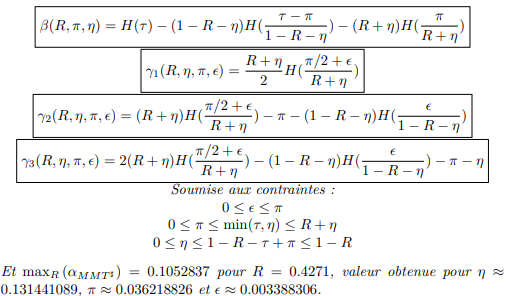
\includegraphics[scale=1.2]{./mmt_diese}
\end{center}


\end{theorem}


Démonstration : Il s'agit des mêmes calculs que pour $ MMT^{\#}  $, à cette différence près qu'il n'y a plus de contrainte de contrainte sur $\epsilon \approx 0.003388306  $.
\subsubsection{Version quantique avec Quantum Walk}
\begin{theorem}\cite{Ghazal} Si H est une matrice aléatoire, en notant  $R:=\frac{k}{n}  $, $\tau :=\frac{t}{n}$,$\pi:=\frac{p}{n} $,$\eta :=\frac{h}{n}$ et $ \epsilon=\frac{\epsilon}{n}$, on a l'expression suivant l'exposant $\alpha_{MMTQW^{\#}} $:
\begin{center}
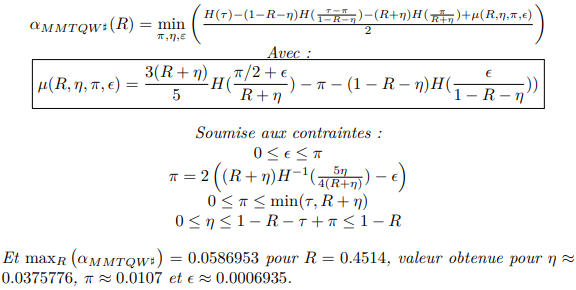
\includegraphics[scale=1.2]{./qw_diese}
\end{center}
\end{theorem}

Démonstration : Il s’agit des mêmes calculs que pour $MMT^{\#}$, à cette différence
près qu’il n’y a plus de contrainte sur $ \epsilon $.\\

L'algorithme de MMT choisit sytématiquement $\epsilon =0  $, ce qui n'est pas optimal. Avec un $\epsilon $ plus grand, on peut diminuer la probabilité de créer des éléments mal formés.Par ailleurs, choisir $\epsilon $ plus grand permet également d'augmenter la taille de l'espace de recherche. Ces deux
considérations vont dans le même sens : il est beaucoup plus facile de trouver
de nombreuses solutions avec $ \epsilon > 0$.\hspace{0.2cm} Cela dit il y'aura alors à nouveau des éléments mal formés. Donc la difficulté consiste à trouver  le bon équilibre. Sur ce, nous attaquons la technique de recherches de voisins proches.

\subsection{Les recherches de voisins proches : Algorithme de  May-Ozerov}
L’algorithme de May et Ozerov
adopte une autre approche : étant donnés deux listes $L_1$ et $L_2$, que l’on a généré
directement ou par collisions/représentations, trouver directement la solution
du problème principal. En termes plus formels, il s’agit de résoudre le problème
du voisin le plus proche mais avant d'énoncer le problème on va définir les 6 lemmes \cite{Ghazal} et les définitions sur lesquels la recherche du voisin le plus se repose:
\begin{definition} Soit $({u^{*}},{v^{*}}) \in L_1 \times L_2 $  la solution cible. On dit qu’un chemin
de la racine jusqu’à une feuille de l’arbre de calcul de NearestNeighbour est bon
si toutes les paires de sous-listes à chaque noeud contiennent $({u^{*}},{v^{*}})$

\end{definition}
\begin{lemme} Soit $(L_1,L_2,\gamma)  $ une instance d'un problème $ Nearest Neighbour $ de paramètres $(m,\gamma,\lambda) $ dont une solution inconnue est $  ( {u^{*}}, {v^{*}} ) \in L_1 \times L_2 $. On écrit $ {u^{*}}=({u^{*}_{1}},\cdots,{u^{*}_{t}})$,${v^{*}}=({v^{*}_{1}},\cdots,{v^{*}_{t}})$ avec chaque ${v^{*}_{j}}, 1 \leq j \leq t  $ sur une bande de longueur $\alpha_i m , \sum_{j=1}^{t}=1$. Alors, il est vrai avec une probabilité inversement
polynomiale que dans au moins une des listes après la permutation uniforme et
l’ajout d’un vecteur $r$ uniformément aléatoire sur chaque bande :
\begin{enumerate}
\item $ w_H({u^{*}_{j}}+ {v^{*}_{j}} )=\gamma \alpha_j m   $
\item $  w_H({u^{*}_{j}} )= w_H({v^{*}_{j}} )= \frac{\gamma \alpha_j m }{2}   , \forall 1 \leq j \leq t $.
\end{enumerate}
\end{lemme}

Le lemme suivant porte sur la probabilité importante que les listes construites
et gardées à chaque étape par l’algorithme $NearestNeighbourRec $ contiennent
la solution cible. On y prouve notamment la nécessité de tester $\tilde{O}(2^{y\alpha_j m})$ à
chaque étape de la récursion.
\begin{lemme} Soit $ t \in \mathbb{N} $ la hauteur de l’arbre de calcul de NearestNeighbour. Alors
cet arbre de calcul comporte un bon chemin avec une probabilité pas trop faible
(inversement polynomiale).
\end{lemme}
Le lemme suivant prouve que le choix d’imposer une limite de taille sur les
listes gardées est pertinente.
\begin{lemme}
Soit $ t \in \mathbb{N} $ la hauteur de l'arbre de calcul de $ NearestNeighbour $ et $\epsilon > 0$.
Alors, parmi les $2t$ listes aux noeuds d’un bon chemin, chacune au niveau $j$ est
de taille {\large $ \tilde{O}\left( 2^{\lambda m (1-\sum_{i=1}^{j}\alpha_i)+\frac{\epsilon}{2}}  \right)  $} avec une probabilité inversement polynomiale.
\end{lemme}
On aura besoin du lemme suivant dans la preuve du théorème final.

\begin{lemme} Soient $0< \gamma < \frac{1}{2}  $ et $ 0 < \lambda < 1-H(\frac{\gamma}{2})$. Soit $y = (1-\gamma)\left( 1-H(\frac{h-\frac{\gamma}{2}}{1-\gamma})  \right)  $ alors $ y>\gamma $

\end{lemme}

\begin{lemme} Soit $ \alpha_1,\cdots,\alpha_t $ une suite de nombres telle que {\large $\alpha_{j+1}=r \alpha_j  $} et {\large $ \sum_{i=1}^{t}\alpha_i=s  $}. Alors {\large $ \alpha_1=\frac{s(1-r)}{1-r^t} $} et {\large $ \alpha_t= \frac{s(1-\frac{1}{r})}{1-(\frac{1}{r})^t}  $}


\end{lemme}

\begin{lemme} 
\begin{enumerate}
\item Si $ \lambda + y \alpha_1 + \frac{\epsilon}{2}   = y+ \epsilon $, alors $ \alpha_1 = \frac{y-\lambda+\frac{\epsilon}{2}}{y}  $

\item Si $\lambda \alpha_t + y + \frac{\epsilon}{2} = y + \epsilon  $, alors $ \alpha_t=\frac{\epsilon}{2 \lambda} $
\end{enumerate}
\end{lemme}


\begin{problem}
Nearest Neighbour de paramètres $(m,\gamma,\lambda) $). Soit $  m \in \mathbb{N}, 0 < \gamma< \frac{1}{2}  $ et $0< \lambda <1 $. Etant donné deux listes $L_1 $, $  L_2$ de taille égale $\mid L_1 \mid= \mid L_2 \mid = 2^{\lambda m} $ de vecteurs uniformément choisis et indépendants deux-à-deux de $\mathbb{F}_{2}^{m}  $, s'il existe $(u* , v*) \in L_1 \times L_2   $ tel que $ w_H(u^{*} + v^{*)}=\gamma m  $, donner une liste $\mathit{C} $ contenant $ (u^{*} , v^{*}) $.\\
Notons qu'un algorithme naïf pour trouver $(u^{*}, v^{*})$ consisterait à tester, pour tous les couples $(u,v)\in L_1 \times L_2 $ s'ils résolvent du problème, i.e. si $ w_H(u + v)=\gamma m  $. Autrement dit, on est à la recherche d'un élément parmi $2^{2\lambda m} $. Ainsi, l'algorithme naïf de résolution du problème coûte $ O(2^{2\lambda m}) $ dans le cas classique et $O(2^{\lambda m})  $ dans le cas quantique avec l'algorithme de grover.

\end{problem}

\subsection{Version classique}
\subsubsection{Algorithme de résolution du problème Nearest Neighbour }

On va donner deux algorithmes : le premier, $NearestNeighbour$, définit
quelques paramètres et initialise un environnement et fait un premier appel
au second algorithme, \\ $ NearestNeighbourRec $ , qui, comme son nom l’indique,
est un algorithme récursif et fait le travail principal de construction de la liste
$ \mathit{C} $, en se basant sur le constat suivant : si on divise longueur $m$ du vecteur en $t$ bandes de longueur  $\alpha_1 m,\cdots, \alpha_t m $, alors si on a $ w_H({u^{*}}+ {v^{*}}) = \gamma m$, on a
aussi, éventuellement après avoir appliqué une même permutation aléatoire aux
coordonnées des vecteurs, que $ w_H({u^{*}_i }+ {v^{*}_i }) = \gamma \alpha_i m$ si $w_i$ désigne la restriction
du vecteur $w$ à la bande de longueur $\gamma \alpha_i m $. Autrement dit, la propriété globale
sur le poids vaut aussi localement sur chaque bande, à quelques nuances près.
\begin{center}
\begin{boxedminipage}[ poslb ]{15cm}

\paragraph{Algorithme 9: $NearestNeighbour $ }\cite{Ghazal}-p85\\

\begin{itemize}
\item[\textbf{Entrées}]: $ L_1,L_2,m,\gamma,h,\lambda,\epsilon $
\item[\textbf{Sorties}]: Liste $ \mathit{C} $ contenant la solution $(u^{*}+ v^{*}) \in L_1 \times L_2  $
\end{itemize}

\begin{enumerate}
\item $ y \gets (1- \gamma)\left( 1- H \left( \frac{H^{-1}(1-\lambda)-\frac{\gamma}{2}}{1-\gamma}  \right) \right)   $

\item $ t \gets \left[ \frac{\log_2(y-\lambda+\frac{\epsilon}{2})-\log_2(\frac{\epsilon}{2})}{\log_2(y)-\log_2(\lambda)}   \right]  $
\item $ \alpha_1 \gets \frac{1-\frac{\lambda}{y}}{1-(\frac{\lambda}{y})^t}  $
\item \textbf{pour} $ j \gets 2 $ à $t$ \textbf{faire}
\item $ \alpha_j \gets \frac{y}{\lambda}\alpha_{j-1}  $
\item $ poly(m) $ permutations uniformément aléatoires  $ \pi $ de $ \left\lbrace  1,\cdots,m \right\rbrace  $ \textbf{faire}
\item \textbf{pour} $poly(m) $ vecteurs uniformément aléatoires $r$ ayant poids $  \frac{\alpha_j m}{2}$ \\ sur chaque bande de longueur $ \alpha_j m $ \textbf{faire}
\item $ \bar{L}_i \gets \pi(L_i)+r $ pour $ i=1,2 $
\item Enlever des $ \bar{L}_i $ les vecteurs de poids différent de $  \frac{\alpha_j m}{2}$ sur chaque bande
\item \textbf{retourner} $NearestNeighbourRec(\bar{L}_1,\bar{L}_2,m,t,\gamma,\lambda,(\alpha_j)_{j=1,\cdots,t},y,h,\epsilon,1)  $

\end{enumerate}


\end{boxedminipage}
\end{center}




\begin{center}
\begin{boxedminipage}[ poslb ]{18cm}

\paragraph{Algorithme 10: $NearestNeighbourRec  $ }\cite{Ghazal}-p85\\


\begin{itemize}
\item[\textbf{Entrées}]: $ L_1^{j-1},L_2^{j-1},m,t,\gamma,\lambda,(\alpha_j)_{j=1,\cdots,t},y,h,\epsilon,1  $
\item[\textbf{Sortie}]: Liste $\mathit{C} $ contenant la solution $(u^{*}, v^{*}) \in L_1 \times L_2  $
\end{itemize}
\begin{enumerate}
\item $\mathit{C} \gets \emptyset $
\item \textbf{si} $ j = t+1  $ \textbf{alors}
/* cas de base
\item $ \mathit{C} \gets \left\lbrace (u,v) \in L_{1}^{(j)} \times L_{2}^{(j)}\hspace{0.3cm} |\hspace{0.3cm} w_H(u+v)=\gamma m \right\rbrace   $
\item \textbf{sinon}
\item  \hspace{0.3cm}\textbf{pour} $\tilde{O(2^{y\alpha_j m})} $ tours de boucle \textbf{faire}
/* cas général
\item \hspace{0.5cm} $ A_j = A_{j,1} \sqcup A_{j,2} \gets $ partition de la bande de longueur $ \alpha_j m  $ en deux parties égales
\item \hspace{0.5cm} \textbf{pour} $i=1,2  $ \textbf{faire}
\item \hspace{0.7cm} $ L_i^{(j)}\gets \left\lbrace v_{L_i^{(j-1)}} \in L_i^{(j-1)} \hspace{0.3cm} \text{de poids} \hspace{0.3cm}\frac{\alpha_j h m}{2} \hspace{0.3cm} \text{sur} \hspace{0.3cm} A_{j,1} \right\rbrace  $

\item \hspace{0.5cm} \textbf{si} $ \mid  L_i^{(j)} \mid \precapprox \tilde{O}\left( 2^{\lambda m(1-\sum_{i=1}^{j}\alpha_i + \frac{\epsilon}{2})} \right)  $ \textbf{alors}
\item \hspace{1cm} $ \mathit{C} \gets \mathit{C}\cup NearestNeighbourRect(L_1^{(j)},L_2^{(j)},m,t,\gamma,\lambda,(\alpha_j)_{j=1,\cdots,t},y,h,\epsilon,j+1)  $



\end{enumerate}

\end{boxedminipage}
\end{center}

Le principe de cette méthode repose sur le théorème suivant:
\begin{theorem} \cite{Ghazal}-p95 Pour tout $\epsilon > 0 $ et $\lambda < 1-\mathit{H}(\frac{\gamma}{2})$, l'algorithme $ NearestNeighbour $ résout le problème Nearest Neighbour de paramètres $(m,\gamma, \lambda) $ avec une probabilité inversement polynomiale en temps $ \tilde{O}(2^{(y+\epsilon)m})  $ où $ y=(1-\gamma)\left( 1 - H(\frac{h-\frac{\gamma}{2}}{1-\gamma}) \right)  $

\end{theorem}
\paragraph{Démonstration : \\}
D'après le lemme 2, l'arbre de calcul de l'algorithme comporte un bon chemin avec une probabilité inversement polynomiale. On considère ce chemin.Alors, d'après le lemme 3, la taille de chaque liste d'entrée au niveau $   j,1 \leq j \leq  t $ est $ \tilde{O}\left( 2^{m(\lambda(1-\sum_{i=1}^{j-1} \alpha_i )+\frac{\epsilon}{2})} \right) $. On construit $\tilde{O}(2^{y\alpha_j m})  $ nouvelles sous-listes à ce niveau,ce qui, par récurrence, donne un total de $ \tilde{O}\left( 2^{y \sum_{i=1}^{j}\alpha_j m}  \right)  $ sous-listes à ce niveau, construites à l’aide d’une procédure de
recherche dans les listes d’entrées. La complexité de calcul au niveau $j$ est donc :
\begin{center}

$ \tilde{O}\left( 2^{m(\lambda(1-\sum_{i=1}^{j-1} \alpha_i )+\frac{\epsilon}{2})} 2^{y \sum_{i=1}^{j}\alpha_j m}  \right)  $\\

$ \tilde{O}\left( 2^{m(\lambda(1-\sum_{i=1}^{j-1} \alpha_i )+\frac{\epsilon}{2}+ y \sum_{i=1}^{j}\alpha_j } \right) $


\end{center}

Au dernier niveau $(j=t+1)$, il y a $\tilde{O}(2^{ym})  $ listes d'entrée de taille $ \tilde{O}\left( 2^{m(\lambda(1-\sum_{i=1}^{t} \alpha_i )+\frac{\epsilon}{2} } \right)=\tilde{O}(2^{\frac{\epsilon}{2}}) $ on construit la liste des solutions de
manière naïve (i.e. complexité quadratique en la taille des listes) à partir de
ces listes, donc la complexité totale à ce niveau est $ \tilde{O}\left( 2^{m(y+\epsilon)} \right) $.\\
La complexité totale sera donc:
\begin{center}
$\max_{j=1,\cdots,t}\left( 2^{m(\lambda(1-\sum_{i=1}^{j-1}\alpha_i)+ y \sum_{i=1}^{j})\alpha_i +\frac{\epsilon}{2})} ,2^{m(y+\epsilon)} \right)  $
\end{center}

D'après le lemme 5, la complexité de tous les étapes dépendant de $j$ seront égales pour le choix de \\
(*) $ \alpha_1 = \frac{1-\frac{\lambda}{y}}{1-({\frac{\lambda}{y}})^{t}}  $ 
avec une valeur de (**) $\tilde{O}\left( 2^{m(\lambda + y \alpha_1)+\frac{\epsilon}{2}} \right)  $\\
Ainsi le lemme 6 permet l'égalité de complexité des j étapes et le dernier étape de l'algorithme en résolvant l'équation suivante:\\

$ (*)=(**) \Rightarrow t=\frac{\log_2(y-\lambda + \frac{\epsilon}{2})-\log_2(\frac{\epsilon}{2})}{\log_2(y)-\log_2(\lambda)} $\\
Cette technique posséde ausssi une version quantique avec l'utilisation de l'algoorithme de $ Grover $ pour effectuer les opérations de recherche mais celui demeure inéfficace à cause de la taille des listes construites. Cependant en utilisant le quantum Walk sur un graphe de Johnson.\\

On a dit que l’on pouvait considérer l’algorithme de May et Ozerov sous forme
d’un arbre de calcul à $ t + 1 $ niveaux numérotés de 0 à $t$ , où à chaque noeud il
y a deux listes $L_j^{(1)}$

et $L_j^{(2)}$
et chaque noeud de niveau $j$ a en moyenne $2^{y \alpha_j m} $
fils. Le but était de trouver un bon chemin, vérifiant certaines propriétés, de la
racine à une feuille.
Ce qu’on a fait avec l’algorithme de Grover consistait à améliorer le temps de
recherche du bons fils à chaque niveau de l’arbre. Illustration 

\begin{center}

\begin{figure}


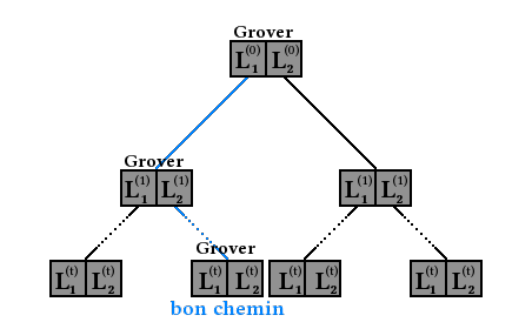
\includegraphics[scale=1]{./nearst_walk}
\caption{ illustration sous forme d'arbre}

\end{figure}
\end{center}


\chapter{Etudes comparatives}
\minitoc
\newpage
Les algorithmes maintenus pour 4 ème tour de NIST ont apporté des améliorations par rapport à leur ancienne version si elle existe soit au niveau de la sécurité , soit dans leur impléméntation. Dans ce chapitre on verra une analogie des avantages et des inconvénients des candidats.

\section{Classic McEliece}
Pou rappel le système de McEliece est muni des paramètres $(n,k,t) $ pour un  $(n,k)$-code linéaire \textbf{C} capable de corriger $t$ partagés par les différentes parties, d'une paire de clef publique 
$({\mathit{G'}},t )$ et privée $(\mathit{S},\mathit{G},\mathit{P})$ tel que $ {\mathit{G'}}=\mathit{S} \mathit{G}\mathit{P} $ avec $ \mathit{S} $ une matrice binaire aléatoire de taille $k \times n   $ non singulier, $\mathit{G} $, une matrice génératrice de \textbf{C} de taille $k \times n  $ et $ P $, une matrice de permutation aléatoire de taille $ n \times n $. \\ Les clés publiques et privée sont de grandes matrices ce qui constitue un des plus grands désavantages. De plus la grandeur du texte chiffré est deux fois celle du texte d'origine.\cite{McEliece2}




\subsection{Avantages}

Le principal avantage de cette méthode est sa facilité d’implémentation :
les seules opérations sont des opérations bit à bit. Par contre, l’implémentation nécessite
beaucoup de place mémoire.\\
Ce cryptosystème, reposant sur un problème difficile de la théorie des codes, n’a pas
rencontré de véritable soutien dans la communauté cryptographique. L’une des principales
raisons de cet état de fait est la taille de la clé. Pourtant, le cryptosystème de McEliece
possède des propriétés intéressantes, citons notamment
\begin{itemize}


\item[-] la sécurité croît beaucoup plus avec la taille des clés que pour le système RSA ;
\item[-] la rapidité du chiffrement.
Un autre avantage est de reposer sur un problème très différent des algorithmes
asymétriques usuels.
\end{itemize}
En conséquence de quoi une percée théorique dans le domaine de la factorisation, qui
ruinerait RSA, n’affecterait en rien ce cryptosystème. Le cryptosystème de McEliece résiste à
ce jour à toute tentative de cryptanalyse, mais est rarement utilisé en pratique du fait de la
grande taille des clés . 

\subsection{Les inconvénients}
\begin{enumerate}


\item La taille de la clef publique posera certainement des problèmes
d'exécution.
\item Le message chiffré est plus long que le message clair. Cette augmentation de la largeur du
message chiffré rend le système plus sensible aux erreurs de transmission.
\item Le crypto système n’est employé pour la signature ou l'authentification parce que
l'algorithme de chiffrage n'est pas linéaire et tout l’algorithme est vraiment asymétrique .

\end{enumerate}
\subsection{Cryptanalyse du système}

La sécurité repose sur l’impossibilité de déduire un algorithme de décodage efficace de la
seule clé publique.\\
Si tel est le cas, le décryptage d’une instance du système se ramènera à la résolution d’une
instance d’un problème de décodage dans un code linéaire. Il en découle que toute attaque du
système devra appartenir à l’une des catégories suivantes :
\begin{itemize}


\item[-] les attaques par décodage : il s’agit de décoder une instance du cryptosystéme à l’aide
d’un algorithme général (i.e. le code public est considère comme un code linéaire aléatoire :  Pour être plus
précis, nous disons que le Goppa distinguishing problem, qui demande de discriminer
si un ensemble de vecteurs est la base d’un code de Goppa ou d’un code aléatoire,
est intraitable du point de vue informatique ).

\item[-] les attaques structurelles : il s’agit, à l’aide de la clé publique, de retrouver tout ou partie
de la structure du code secret.
\end{itemize}
\section{BIKE}
BIKE est une suite de mécanismes d'encapsulation de clé sécurisée (KEM) IND-CPA composée de BIKE-1, BIKE-2 et BIKE-3. Chaque variante a son
propres avantages et inconvénients.\\ \cite{Rap}
\subsection{Les avantages}
\begin{enumerate}
\item  toutes les variantes de BIKE sont basées sur une densité modérée quasi-cyclique
contrôle de parité (codes QC-MDPC), qui peuvent être décodés efficacement grâce à des techniques de décodage par retournement de bits. Ce type de décodeur est extrêmement simple : il estime
quelles sont les positions les plus susceptibles d'être erronées, retournez-les et observez si le résultat est meilleur (poids du syndrome plus petit) qu'avant ou non. Ce processus converge
très rapidement; en particulier, on a présenté un décodeur à retournement de bits à 1 itération.
\item Une autre caractéristique commune à toutes les variantes de BIKE est le fait qu'elles s'appuient 
sur des clés éphémères. Cela conduit à deux choses : dans un premier temps, cela va à l’encontre du GJS.
attaque de réaction mentionnée dans la section 5, qui est une attaque qui doit être observée
un grand nombre de décodages pour une même clé privée (chose impossible quand
des clés éphémères sont utilisées). L'autre aspect de ce choix est que la génération clé
doit être efficace puisqu’il est exécuté à chaque encapsulation de clé.

\item Concernant la bande passante de communication, dans BIKE-1 et BIKE-3 toutes les clés publiques,
les clés privées et les cryptogrammes ont une longueur de n bits, correspondant à la bande passante
des messages échangés par les parties. BIKE-2 propose des clés publiques plus petites et
textes chiffrés, r bits uniquement, correspondant à la bande passante des messages échangés
également par les parties. Deux messages sont échangés par encapsulation de clé de celui-ci
taille (soit n, soit r bits). En pratique, ces chiffres vont de 1,24 Ko par message
en BIKE-2 niveau de sécurité 1, jusqu'à 8,82 Ko par message en BIKE-3 niveau de sécurité 5.
Ces chiffres semblent assez raisonnables par rapport à la taille moyenne d'un
page sur Internet (actuellement près de 2 Mo [2]), à titre d'exemple 
\end{enumerate}
 


\subsection{Les incovénients}

\begin{enumerate}



\item Un point d'attention dans BIKE est le fait que, de nos jours, le bit flipping
les techniques de décodage n'atteignent pas un taux d'échec de décodage négligeable. Cela fait
défi pour atteindre des notions de sécurité plus élevées telles que IND-CCA. Cela peut également limiter
l'utilisation de BIKE dans certaines applications comme par exemple Hybrid Encryption,
où KEM et DEM doivent tous deux satisfaire à la sécurité IND-CCA pour garantir la sécurité du texte chiffré choisi pour le schéma de chiffrement hybride. Nous soulignons cependant qu'il
semble possible (mais pas simple) de prouver que certaines techniques de décodage peuvent
en fait, ils atteignent des taux d'échec de décodage négligeables pour les codes QC-MDPC.

\item Concernant la propriété intellectuelle, au meilleur de nos connaissances, BIKE-1 et
BIKE-2 n’est couvert par aucun brevet. BIKE-3 est couvert par un brevet dont
les propriétaires sont disposés à accorder une licence non exclusive aux fins de mise en œuvre
la norme sans compensation et selon des termes et conditions raisonnables qui
sont manifestement exempts de toute discrimination injuste, comme indiqué dans les documents ci-joints.
déclarations signées. Nous soulignons que BIKE-1 et BIKE-2 ne sont pas couverts par
le brevet susmentionné, et que l'équipe BIKE est prête à abandonner BIKE-3 si
cela devient toujours un inconvénient lorsque l'on compare notre suite avec d'autres propositions.

\end{enumerate}

\subsection{Cryptanalyse du système}

\begin{enumerate}


\item Concernant la sécurité, toutes les variantes de BIKE s'appuient sur des
problèmes de théorie du codage : problèmes de décodage du syndrome quasi-cyclique et de recherche de mots de code quasi-cycliques. Les meilleures stratégies pour résoudre ces problèmes reposent sur les techniques de décodage des ensembles d'informations (ISD), un domaine de recherche qui existe depuis très longtemps.
historique (l’ouvrage fondateur de Prange remonte à 1962) et qui semble très peu
amélioration au fil des années. De plus, nous montrons que dans le cadre quantique,
L’algorithme de Grover utilisé en plus de l’algorithme séminal de Prange ISD est toujours le
choix le plus préférable dans notre cas.


\item "BIKE cible la sécurité de l'IND-CPA et ne tente pas d'y parvenir
difficile pour un attaquant de lancer une attaque par texte chiffré choisi si les clés sont
réutilisé. Cette décision de conception a été prise par les auteurs, sur la base des
difficulté de concevoir un décodeur bit-flipping avec un signal suffisamment faible
taux d'échec de décodage pour permettre une sécurité IND-CCA2 efficace
construction."
\item  La meilleure attaque ISD est Prange qui le fait en 50 ans

\end{enumerate}
Dans la sécurité pratique les meilleures attaques connues sont \cite{Rap} :
\begin{itemize}
\item[\textbf{-key distinguisting attack :}] qui trouve un mot chiffré de $ \mathit{C}^{\perp} $ de poids $w$ dans ce cas l’adversaire applique un isd sur le syndrome et la matrice de contôle de parité pour aboutir à la résolution d’un problème avec $r$ solutions telles r soit le nombre de lignes creuses de la amtrice de contrôle de parité. Pour $ N_s=r$ et $N_i=1$ , le coût de l’attaque diminue d’un facteur :

$ WF_{dist}(n,r,w)=WFisd(n,n-r,w)/r $ 

Dans le cas quasi-cyclique, il n’y a pas d’accélération évidente et on distingue
l'attaque a le même coût que ci-dessus.

\item[\textbf{-key recovery attack :}] qui trouve $r$ mots chiffrés de $ \mathit{C}^{\perp} $ de poids $w$

Dans ce cas on veut estimer le coût $WF_{reco}(n,r,w)$ de l’attaque en produisant r mots cachés de poids $w$ dans $ \mathit{C}^{\perp} $.  On applique aléatoirement r attaques ISD pour trouver un mot .\hspace{0.2cm} Sur chaque attaque a en moyenne $\frac{WF_{isd}(n,n-r,w)}{r}$ puisqu’il y’a $r$ mots codés de poids $w$ .Donc le coût de l’ensemble est :
\begin{center}
{\large

$WF_{reco}(n,n-r,w)=r \cdot \frac{WF_{isd}(n,n-r,w)}{r} 
= \frac{WF_{isd}(n,n-r,w)}{r}$}

\end{center}

Dans l’utilisation des codes quasi-cycliques tous les mots de poids faibles peuvent être retrouvés et l’attaque de key recovery attack n’est plus coûteuse que le key distinguishing attaque.
\begin{center}

{\large
$WF_{reco}^{QC}(n,r,w)= WF_{dist}^{QC}(n,r,w)= \frac{ WF_{isd}(n,n-r,w)}{r}$}.
\end{center}

\item[ \textbf{-Decoding attack :}]qui décode $t$ erreurs d’un $ (n , n-r)-code linéaire  $.

Soit une estimation du coût de l’attaque  $ WF_{dect}(n,r,t) $  pour décoder $t$ erreurs.
Dans le cas des codes MDPC on a :\begin{center}

 {\large $  WF_{dec}(n,r,t)=WF_{isd}(n,r,t)    $} .
 \end{center}

Dans le cas quasi-cyclique, tout déplacement cyclique du syndrome cible  $  s \in \mathbb{F}_{2}^{r}  $
fournit une nouvelle instance dont la solution est égale à l'originale, à une précision près
décalage cyclique par bloc. Ainsi le nombre d'instances et de solutions est
$N_i = N_s = r $ . Donc un facteur $ \sqrt{r} $ est gagné :
\begin{center}

{\large

$ WF_{reco}^{QC}(n,r,t)\geq \frac{WF_{isd}(n,r,t)}{ \sqrt{r}}  $}
\hspace{0.3cm}
\end{center}
\begin{table}
\centering
\begin{tabular}{|R{5cm}||C{4cm}|L{4cm}|L{4.5cm}|}
\hline  & MDPC &  QC-MDPC \\
\hline  Key distinguishing  &$ \frac{1}{r}WF_{isd}(n,n-r,w) $ & $\frac{1}{r}WF_{isd}(n,n-r,w) $  \\
\hline 
Key recovery  &$ WF_{isd}(n,n-r,w) $ & $\frac{1}{r}WF_{isd}(n,n-r,w) $  \\
Decoding  &$ WF_{isd}(n,r,t) $ & $\frac{1}{\sqrt{r}}WF_{isd}(n,r,t) $  \\
\hline

\end{tabular}
\caption{Les meilleures attaques contre MDPC (or QC-MDPC) codes }
\label{tab5}
\end{table}

\end{itemize}
\hspace{1.2cm}
La dernière est le cas de Decoding One Out Of Many (DOOM), l'attaquant analyse le gain ( le gain réel pourrait être légèrement inférieur, puisque ces algorithmes dépendent de
paramètres optimaux qui peuvent ne pas être les mêmes pour plusieurs instances) lorsque le problème de décodage est résolu
plusieurs solutions et l’adversaire se contente d’en trouver une seule.
En bref, lorsque le problème a $N_s$ solutions, la probabilité de succès $\mathit{P}$
augmente d'un facteur $N_s$ (tant que $N_s P \ll 1 $)
et quand $N_i  $ les instances sont traitées
simultanément, la taille de la liste $\mathbf{L}$ augmente au maximum d'un facteur $\sqrt{N_i}  $ donc:\\
La technique DOOM apporte un gain de $N_s / \sqrt{N_i}$ 

Pour toutes les attaques, nous devons résoudre le problème du décodage par syndrôme. La meilleure technique est le décodage d'ensembles d'informations (ISD).
Les facteurs de travail ISD sont couramment utilisés pour l'évaluation de la sécurité des systèmes basés sur le code.


\section{Hamming quasi-cyclic}

Hamming Quasi-Cyclic (HQC) est un algorithme cryptographique post-quantique qui présente ses propres avantages et inconvénients. Explorons-les en fonction des informations disponibles.
\subsection{Les avantages}
\begin{enumerate}
\item Sécurité contre les attaques quantiques : HQC est conçu pour résister aux attaques des ordinateurs quantiques. À mesure que les ordinateurs quantiques deviennent plus puissants, les algorithmes cryptographiques traditionnels peuvent devenir vulnérables, faisant du HQC une solution importante pour sécuriser les communications à l'ère post-quantique.
\item Implémentation efficace : HQC offre une implémentation relativement efficace par rapport aux autres algorithmes post-quantiques. Il offre un bon équilibre entre sécurité et performances, ce qui le rend adapté à divers cas d'utilisation.
\item Aucune structure cachée : HQC ne s'appuie pas sur des structures cachées dans son processus de cryptage, ce qui ajoute une couche de sécurité supplémentaire. Cette résilience face à la cryptanalyse fait du HQC une option prometteuse pour des communications sécurisées.

\end{enumerate}
\subsection{Les inconvénients}

\begin{enumerate}
\item Taille de clé de chiffrement plus petite : comparé à certains autres algorithmes cryptographiques post-quantiques, HQC a une taille de clé de chiffrement plus petite. Cela peut limiter son caractère pratique dans certains scénarios où des clés plus grandes peuvent être souhaitées pour une sécurité renforcée.
\item Adoption et recherche limitées : HQC est un algorithme relativement nouveau dans le domaine de la cryptographie post-quantique, ce qui signifie qu'il n'a pas encore été largement adopté et n'a pas fait l'objet de recherches approfondies. Cela peut entraîner une certaine incertitude quant à la sécurité et à la maturité à long terme de l'algorithme.
\end{enumerate}
Il convient de noter que le domaine de la cryptographie post-quantique est en constante évolution et que de nouvelles recherches et développements pourraient affecter les avantages et les inconvénients du HQC à l'avenir.\\

Nous avons vu que les algorithmes ISD classiques et quantiques sont  jusque là les meilleures attaques sur nos candidats malgré que la complexité soit toujours exponentielle. Cependant l'informatique quantique apporte aussi une perspective en ce sens.

\begin{table}
\centering

\begin{tabular}{|c||c|c|c|c|c|} 
\hline

\multicolumn{1}{|c||}{} &  \multicolumn{1}{c|}{Classic Mc Eliece}&  \multicolumn{3}{c|}{Bike}&  \multicolumn{1}{c|}{HQC} \\ 
 \hline
 \cline{3-5}
Niveau &         & I &  II &   III &    \\
\hline
clé public & 1044992 & 8188 & 4094 & 9033 & 4616 \\
\hline
clé privée & 13892 & 548 & 548 & 532 & 764 \\
\hline
Chiffré & 240 & 8188 & 4094 & 9033 & 4616 \\
\hline
 
\end{tabular}
\caption{Tableau comparatif des candidats sur le niveau de sécurité 5}
\label{comparatif}

\end{table}
\chapter{Quelques implémentations }

\chapter{Conclusion et Perspectives}

Au terme de notre recherche nous avons vu que le NIST (National Institut of Standardization and Technology) a lancé son concours international dans l'optique de sélectionner les meilleurs algorithmes chiffrements post-quantiques basés sur les codes correcteurs d'erreur capables de résister à la puissance de la machine quantique.\\
De cette compétition qui était à son 3 tours en 2021, il a été retenu 3 candidats qui sont le classic McEliece,Bike (Bit flipping key encryption),Hamming quasi-cyclic suivant les critères (la sécurité,la performance, la flexibilité,la simplicité de mise en oeuvre et la qualité des implémentations proposées). Chacun a ses avantages et ses inconvénients.\\
Premièrement parlant de classic McEliece, il est fait à partir des codes de Goppa binaire. Il posséde le couple  $  (  \tilde{G},t  )$ comme clé publique tels que $ \tilde{G}=[I_{n-k}|A]$ une matrice systèmatique avec $ t$, le poids de Hamming du vecteur à chiffrer et $ (s, \Gamma)   $, sa clef privée telles $s$, une chaîne aléatoire de n-bits et $  \Gamma=(g,\alpha_1,\cdots,\alpha_n)   $ avec $g$ , un polynôme minimal irréductible et $  \alpha_1,\cdots,\alpha_n  $ , n éléments deux à deux distincts dans $ \mathbb{F}_q   $








Du point de vue de la sécurité les meilleures attaques ont une complexité exponentielle à l'instar des attaques de décodage par ensemble d'information(ISD)classiques et quantiques. Celles-ci se basant sur diverses méthodologies à savoir avec technique de représentation ou répresentation étendue ou bien par la recherche du voisin le plus proche (Nearst Neighboor) tendent à réduire cette complexité exponentielle dont l'exposant est appelé exposant de Prange.Ainsi les meilleurs ISD sont quantiques imbriquant l'algorithme de Grover qui a une complexité $\mathit{O}(\sqrt{N})  $ avec $N=2^n $.Ces ISD ont donnent une réduction quadratique de l'exposant de Prange.
Cependant face au développement fulgurant du monde de la technologie et des réseaux il est opportun que l'on pense à ébaucher de nouveaux circuits classiques implémentant des candidats.

\begin{thebibliography}{1}


\baselineskip=10pt



 \bibitem{aragonbike} N. Aragon, P. S. L. M. Barreto, S. Bettaieb, L. Bidoux, O. Blazy, J.-C.
Deneuville, P. Gaborit, S. Gueron, T. G¨uneysu, C. A. Melchor, R. Misoczki,
E. Persichetti, N. Sendrier, J.-P. Tillich, V. Vasseur, and G. Z´emor, “BIKE:
Bit Flipping Key Encapsulation Round 3 Submission.” Available online: https:
//bikesuite.org/, 2020. Accessed on 17 February 2020\\


 \bibitem{aragon20} N. Aragon, P. S. L. M. Barreto, S. Bettaieb, L. Bidoux, O. Blazy, J.-C.
Deneuville, P. Gaborit, S. Gueron, T. G¨uneysu, C. A. Melchor, R. Misoczki,
E. Persichetti, N. Sendrier, J.-P. Tillich, V. Vasseur, and G. Z´emor, “BIKE:
Bit Flipping Key Encapsulation Round 3 Submission.” Available online: https:$
//bikesuite.org/files/v4.0/BIKE_Spec.2020.05.03.1.pdf, 2020. Accessed
on 23 May 2020.$\\





\bibitem{Bernstein} D. J. Bernstein, T. Chou, T. Lange, R. Misoczki, R. Niederhagen, E. Persichetti, P. Schwabe, J. Szefer, and W. Wang, “Classic
McEliece: Conservative Code-based Cryptography 30 March 2019.” https:
//csrc.nist.gov/csrc/media/projects/post-quantum-cryptography/\\


\bibitem{berns2010} D. J. Bernstein, “Grover vs. McEliece,” in International Workshop on PostQuantum Cryptography (PQCRYPTO), vol. 6061 of Lecture Notes in Computer Science, pp. 73–80, Springer, 2010. \\


\bibitem{Daniel} Daniel J. Bernstein, Tung Chou, and Peter Schwabe. McBits: Fast constant-time code based cryptography. In Guido Bertoni and Jean-S´ebastien Coron, editors, Cryptographic
Hardware and Embedded Systems - CHES 2013 - 15th International Workshop, Santa
Barbara, CA, USA, August 20-23, 2013. Proceedings, volume 8086 of Lecture Notes in
Computer Science, pages 250–272. Springer, 2013.\\

\bibitem{Bernstein6} Bernstein, D. J., Jeffery, S., Lange, T., and Meurer, A. Quantum algorithms for the subset sum problem. In Post-Quantum Cryptography 2011 (Limoges, France, June 2013), vol. 7932 of Lectur\\

\bibitem{desmarais} John-Marc Desmarais 
"Error Correcting Codes in Post-Quantum Cryptography"  A thesis submitted to the Faculty of Graduate Studies and Research in partial fulfilment of the requirements for the degree of Master of Science Ottawa Carleton Institute Aug. 2020\\

{\it Department of Mathematics
Carleton University
Ottawa, Ontario, Canada
August 2020} \\

\bibitem{druckergueron2020} N. Drucker, S. Gueron, and D. Kostic, “Fast Polynomial Inversion for Post Quantum QC-MDPC Cryptography,” IACR Cryptol. ePrint Arch., vol. 2020, p. 298,2020.\\

 \bibitem{gallager63} R. G. Gallager. Low- Density-Parity-Check Codes M.I.T Press, 1963 \\

\bibitem{Grenet} Bruno Grenet , {\em Introduction aux algorithmes probabilistes}, Septembre 2018. \\


\bibitem{itoh88} T. Itoh and S. Tsujii, \textit{“A Fast Algorithm for Computing Multiplicative Inverses
in GF (2m) Using Normal Bases,”}  Information and Computation, vol. 78, no. 3,
pp. 171–177, 1988.\\



\bibitem{prange62}  E. Prange, “The Use of Information Sets in Decoding Cyclic Codes,” IRE Transactions on Information Theory, vol. 8, no. 5, pp. 5-9, 1962.\\



 

\bibitem{drucker2019} N. Drucker, S. Gueron, and D. Kostic, “QC-MDPC Decoders with Several Shades
of Gray,”\textit{in International Conference on Post-Quantum Cryptography, vol. 12100} of Lecture Notes in Computer Science, pp. 35–50, Springer, 2020.\\


\bibitem{Dumer11} Dumer, I. On minimum distance decoding of linear codes. In Proc. 5th Joint Soviet-Swedish Int.
Workshop Inform. Theory (Moscow, 1991), pp. 50–52.\\



\bibitem{drucker2019} N. Drucker, S. Gueron, and D. Kostic, “On Constant-time QC-MDPC Decoding with Negligible Failure Rate,” Technical Report, Cryptology ePrint Archive,
Report 2019/1289, 2019.\\

\bibitem{aragon2020} N. Aragon, P. S. L. M. Barreto, S. Bettaieb, L. Bidoux, O. Blazy, J.-C.
Deneuville, P. Gaborit, S. Gueron, T. G¨uneysu, C. A. Melchor, R. Misoczki,
E. Persichetti, N. Sendrier, J.-P. Tillich, V. Vasseur, and G. Z´emor, “BIKE:
Bit Flipping Key Encapsulation Round 3 Submission.” Available $online: https:
//bikesuite.org/files/v4.0/BIKE_Spec.2020.05.03.1.pdf, 2020. Accessed
on 23 May 2020.$ \\

\bibitem{chaulet2017} J. Chaulet, Etude de cryptosystèmes à clé publique basés sur les codes MDPC quasi-cycliques. PhD thesis, Paris 6, 2017.\\

\bibitem{aragon2020}N. Aragon, P. S. L. M. Barreto, S. Bettaieb, L. Bidoux, O. Blazy, J.-C.Deneuville, P. Gaborit, S. Gueron, T. G¨uneysu, C. A. Melchor, R. Misoczki,E. Persichetti, N. Sendrier, J.-P. Tillich, and G. Z´emor, “BIKE: Bit Flipping Key Encapsulation Round 1 Submission.” Available online:$ https://bikesuite.org/, 2017. Accessed on 5 July 2020.$\\


\bibitem{baldi2014} M. Baldi, QC-LDPC Code-based Cryptography. Springer Science and Business,2014.\\



\bibitem{Bjmm2} A. Becker, A. Joux, A. May, A. Meurer: “Decoding random binary linear codes in 2n/20: $How 1 + 1 = 0$ improves information set decoding”, In Annual international conference on the theory and applications of cryptographic techniques, pp.520–536, 2012.\\




\bibitem{Bergrover3} D. J. Bernstein: “Grover vs. McEliece”, In Post-Quantum Cryptography 2010 (2010),
N. Sendrier,Ed., vol.6061 of Lecture Notes in Comput. Sci., Springer, pp.73–80, 2010.\\

\bibitem{berlekamp1978} E. Berlekamp, R. McEliece, and H. Van Tilborg, “On the Inherent Intractability of Certain Coding Problems,” IEEE Transactions on Information Theory,vol. $24, no. 3, pp. 384–386, 1978.$\\

\bibitem{Ndollane} Gilbert N. Dione, \it{Schéma d'identification et Mécanisme d'encapsulation de clé},Thèse de doctorat Unique,Université Cheikh A. DIOP, 30 novembre 2020 \\

\bibitem{drucker2019} N. Drucker, S. Gueron, and D. Kostic, “ On Constant-time QC-MDPC Decoding with Negligible Failure Rate”, Technical Report, Cryptology ePrint Archive, Report $2019/1289, 2019.$\\

\bibitem{Belestr5} A. Esser, E. Bellini: “Syndrome decoding estimator”, In: IACR International Conference on Public-Key Cryptography. Springer, Cham, pp.112-141, 2022 \\

\bibitem{Essramos6}  A. Esser, S. Ramos-Calderer, E. Bellini, J. I. Latorre, M. Manzano: “Hybrid
Decoding–Classical-Quantum Trade-Offs for Information Set Decoding”, Cryptology ePrint Archive, 2022.\\


\bibitem{Kati9} G. Kachigar and J.P. Tillich: “Quantum information set decoding algorithms”, In:
International Workshop on Post-Quantum Cryptography. Springer, Cham, pp.69-89, 2017\\



\bibitem{Leebr10} P. Lee and E. Brickell: “An observation on the security of McEliece’s public-key
cryptosystem”, In Advances in Cryptology―EUROCRYPT’88, C. Günter, Ed. New
York: Springer-Verlag, p.275, 1988.\\


\bibitem{londahl2016} C. Londahl, T. Johansson, M. K. Shooshtari, M. Ahmadian-Attari, and M. R. Aref, “Squaring Attacks on McEliece Public-key Cryptosystems Using Quasi cyclic Codes of Even Dimension,” Designs, Codes and Cryptography, vol.$ 80, no. 2, pp. 359–377, 2016.$\\

\bibitem{ibra09} Mr Ibrahima MBAYE, Memoire de DEA Mathématiques, \it{LA Théorie des codes correcteurs d'erreurs}, 18 juillet 2009
 \\

 
 \bibitem{misoczk13i} R. Misoczki, J. -P. Tillich, N. Sendrier, and P. S. L. M. Barreta, "MDPCMcEliece: New McEliece variants from moderate density parity-check codes," \it{ in Proc, IEEE Int. Symposium Inf: Theory - ISIT , 2013 } , pp. 2069-2073\\
 

\bibitem{Mmt11} A. May, A. Meurer, E. Thomae: “Decoding random linear codes in O˜(20.054n)”, In International Conference on the Theory and Application of Cryptology and Information Security, pp.107–124, 2011\\

\bibitem{Mo19} May, A., and Ozerov, I. On computing nearest neighbors with applications to decoding of binary
linear codes. In Advances in Cryptology - EUROCRYPT 2015 (2015), E. Oswald and M. Fischlin,
Eds., vol. 9056 of Lecture Notes in Comput. Sci., Springer, pp. 203–228.\\

\bibitem{McEliece2} R.J. McEliece, {\em A public-key cryptosystem based on algebraic coding theory}, JPL DSN Progress Report 4244 (1978), 114-116. \\


\bibitem{melchor2020} C. A. Melchor, N. Aragon, S. Bettaieb, L. Bidoux, O. Blazy, J. Bos, J.-C.
Deneuville, P. Gaborit, E. Persichetti, J.-M. Robert, P. V´eron, and G. Z´emor,\it{“Hamming Quasi-Cyclic (HQC),” Technical Report, National Institute of Standards and Technology 2017, 2020}.\\





\bibitem{Narisada15} S. Narisada, K. Fukushima, S. Kiyomoto: “Multi-Parallel MMT Algorithm for Solving High-Dimensional SDP”, The 2022 Symposium on Cryptography and Information Security SCIS2022, 4A2-1, 2022.\\




\bibitem{overbeck2020} R. Overbeck, Public Key Cryptography Based on Coding Theory. PhD thesis,\it{Technische Universit¨at, 2007. Retrieved March 3, 2020}.\\


\bibitem{Perriello18} S. Perriello, A. Barenghi, G. Pelosi: “A complete quantum circuit to solve the information set decoding problem”, In: 2021 IEEE International Conference on Quantum Computing and Engineering (QCE). IEEE, pp.366-377, 2021.\\

\bibitem{Shannon}  C. E. Shannon, “A mathematical theory of communication, ”Bell Systems Technical Journal, $vol. 27, pp. 379–423,623–656, July 1948.$ \\


\bibitem{charlesfer2004} Charles, S., Ferreol, M., Chaumot, A., et Pery, A.R.R.
(2004) Food availability effect on population dynamics of the midge{\it Chironomus riparius}: a Leslie modeling approach. {\it Ecological Modelling}, {\bf 175}, 217-229.\\









\bibitem{Prange23} Prange, E. The use of information sets in decoding cyclic codes. IRE Transactions on Information
Theory 8, 5 (1962), 5–9\\


\bibitem{ANSSI}  www.ssi.gouv.fr/actualite/selection-par-le-nist-de-futurs-standards-en-cryptographie-post-quantique/ \\


\end{thebibliography}




\end{document}